%%%%%%%%%%%%%%%%%%% vorlage.tex %%%%%%%%%%%%%%%%%%%%%%%%%%%%%
%
% LaTeX-Vorlage zur Erstellung von Projekt-Dokumentationen
% im Fachbereich Informatik der Hochschule Trier
%
% Basis: Vorlage svmono des Springer Verlags
%
%%%%%%%%%%%%%%%%%%%%%%%%%%%%%%%%%%%%%%%%%%%%%%%%%%%%%%%%%%%%%

\documentclass[envcountsame,envcountchap, deutsch]{i-studis}

\usepackage{footnote}
\usepackage[LGR,T1]{fontenc}
\usepackage{float}
\usepackage{python}
\usepackage{xparse}
\usepackage{enumitem}
\usepackage[outputdir=../../auxil]{minted}
\usepackage{comment}
\usepackage{ulem}
\usepackage[inkscapeformat=png]{svg}
\usepackage[titles]{tocloft}
\usepackage{titlesec}
\usepackage{xurl}
\usepackage[titletoc,title,page, header]{appendix} % Anhang
\usepackage[backend=biber, style=alphabetic, isbn=true, doi=true]{biblatex}
\usepackage{makeidx}         	% Index
\usepackage{multicol}% Zweispaltiger Index
\usepackage[threshold=0]{csquotes}
\usepackage{soul}
\usepackage{caption}

\setcounter{tocdepth}{4}
\setcounter{secnumdepth}{6}
\captionsetup{font=small}
\captionsetup{labelfont=bf}

\newtheorem{theorem}{Theorem}
\newcommand{\textgreek}[1]{\begingroup\fontencoding{LGR}\selectfont#1\endgroup}

\BeforeBeginEnvironment{tcolorbox}{\savenotes}
\AfterEndEnvironment{tcolorbox}{\spewnotes}

%\usepackage[bottom]{footmisc}	% Erzeugung von Fu�noten

%%-----------------------------------------------------
%\newif\ifpdf
%\ifx\pdfoutput\undefined
%\pdffalse
%\else
%\pdfoutput=1
%\pdftrue
%\fi
%%--------------------------------------------------------
%\ifpdf
\usepackage[pdftex]{graphicx}
\usepackage{epstopdf}

\usepackage{tcolorbox}
\usepackage[pdftex,plainpages=false]{hyperref}
\usepackage[table]{colortbl}% http://ctan.org/pkg/xcolor
%\else
%\usepackage{graphicx}
%\usepackage[plainpages=false]{hyperref}
%\fi

%%-----------------------------------------------------
\usepackage{color}				% Farbverwaltung
%\usepackage{ngerman} 			% Neue deutsche Rechtsschreibung
\usepackage[english, ngerman]{babel}

\renewcommand\appendixpagename{Anhänge}
\renewcommand\appendixtocname{Anhänge}
%%-----------------------------------------------------
% Unterscheidung für Umlaute Windows-Mac
%%-----------------------------------------------------

%\usepackage[latin1]{inputenc} 	% Ermöglicht Umlaute-Darstellung
\usepackage[utf8]{inputenc}  	% Ermöglicht Umlaute-Darstellung unter Linux (je nach verwendetem Format)

%-----------------------------------------------------
\usepackage{listings} 			% Code-Darstellung
\lstset
{
	basicstyle=\scriptsize, 	% print whole listing small
	keywordstyle=\color{blue}\bfseries,
								% underlined bold black keywords
	identifierstyle=, 			% nothing happens
	commentstyle=\color{red}, 	% white comments
	stringstyle=\ttfamily, 		% typewriter type for strings
	showstringspaces=false, 	% no special string spaces
	framexleftmargin=7mm,
	tabsize=3,
	showtabs=false,
	captionpos=b,
	frame=single,
	rulesepcolor=\color{blue},
	numbers=left,
	linewidth=146mm,
	xleftmargin=8mm
}

\NewDocumentCommand{\code}{v}{%
	\texttt{\textcolor{blue}{#1}}%
}
\NewDocumentCommand{\staticcode}{v}{%
	\ul{{\texttt{\textcolor{blue}{#1}}}}%
}



\usepackage{textcomp} 			% Celsius-Darstellung
\usepackage{amssymb,amsfonts,amstext,amsmath}	% Mathematische Symbole
\usepackage[german, ruled, vlined]{algorithm2e}
\usepackage[a4paper]{geometry} % Andere Formatierung
\usepackage{bibgerm}
\usepackage{array}
\usepackage{lstmisc}
\usepackage[thmarks]{ntheorem}
\usepackage{mathtools}
\hyphenation{Ele-men-tar-ob-jek-te  ab-ge-tas-tet Aus-wer-tung House-holder-Matrix Le-ast-Squa-res-Al-go-ri-th-men} 		% Weitere Silbentrennung bei Bedarf angeben
\setlength{\textheight}{1.1\textheight}
\pagestyle{myheadings} 			% Erzeugt selbstdefinierte Kopfzeile
\makeindex 						% Index-Erstellung

% uncomment to hide tables, equations and figures
%\excludecomment{confidential}
%\excludecomment{figure}
%\excludecomment{equation}
%\excludecomment{table}
%\let\endfigure\relax
%\let\endtable\relax
%\let\endequation\relax


\DeclareFieldFormat{doi}{\textsc{doi}: \texttt{#1}}
\DeclareFieldFormat{isbn}{\textsc{isbn}: \texttt{#1}}

\DeclareFieldFormat{postnote}{#1}
\DeclareFieldFormat{multipostnote}{#1}

\addbibresource{literatur.bib}


%--------------------------------------------------------------------------
\begin{document}
%------------------------- Titelblatt -------------------------------------
\title{\begin{center}
		   Repetitorium FOPT

		   \textbf{}\\
\\

		   \\
		   \small{Modul fopt, WS23/24} \\ \small{Trier University of Applied Sciences}\\ \small{Informatik Fernstudium (M.C.Sc.)}
\end{center}}
\project{}
%--------------------------------------------------------------------------
\supervisor{Titel Vorname Name} 		% Betreuer der Arbeit
\author{\begin{center}

\end{center}}							% Autor der Arbeit
\address{\begin{center}
			 \small{14.02.2024\\  Thorsten Suckow-Homberg, \url{https://thorsten.suckow-homberg.de}}
\end{center}} 							% Im Zusammenhang mit dem Datum wird hinter dem Ort ein Komma angegeben
\submitdate{} 				% Abgabedatum
%\begingroup
%  \renewcommand{\thepage}{title}
%  \mytitlepage
%  \newpage
%\endgroup



\begingroup
  \renewcommand{\thepage}{Titel}
  \mytitlepage
  \newpage
\endgroup
%--------------------------------------------------------------------------
\frontmatter
%--------------------------------------------------------------------------
\Hinweise

Das Repetitorium enthält Notizen und Zitate aus \cite[]{Oec22}, die mir während der Arbeit mit dem Buch als besonders wichtig erschienen.

Einige Abbildungen aus dem Buch wurden zitiert, einige wurden ergänzt bzw. neu erstellt.
Einige Stellen, die im Buch sehr unscharf formuliert sind, wurden in dieser Zusammenfassung besonders markiert.

Das Repetitorium versteht sich nicht als Ersatz zu dem Buch bzw. den Skripten, sondern als Ergänzung zur Prüfungsvorbereitung.
\tableofcontents 						% Inhaltsverzeichnis
%--------------------------------------------------------------------------
\mainmatter                        		% Hauptteil (ab hier arab. Seitenzahlen)
%--------------------------------------------------------------------------
% Die Kapitel werden in separaten .tex-Dateien abgelegt und hier eingebunden.

\begin{appendices}
    
\begin{appendices}
    
\begin{appendices}
    \input{chapters/Anhang/Zusatzaufgaben/index}
    \input{chapters/Anhang/Klausuren/ws13}
    \input{chapters/Anhang/Klausuren/ws15-16}
    \input{chapters/Anhang/Klausuren/ws16-17}
    \input{chapters/Anhang/Klausuren/ss19}
    \input{chapters/Anhang/Präsenzphase/index}

\end{appendices}

    \chapter{WS13}\label{ch:klausurws13}

\section{Aufgabe 1}
\subsection{Lösungsvorschlag}


\begin{minted}[mathescape,
    linenos,
    numbersep=5pt,
    gobble=2,
    fontsize=\small,
    frame=lines,
    framesep=2mm]{java}
    class Zahlenschloss {

        private int[] kombination;

        private int[] state;

        private boolean opened = false;

        public Zahlenschloss(int[] kombination) {
            this.kombination = kombination;
            this.state = new int[kombination.length];
        }

        public int anzahlRaedchen() {
            return kombination.length;
        }

        public synchronized int lesen(int radnummer) {
            return state[radnummer];
        }

        public synchronized void drehen(int radnummer, int zahl) {

            state[radnummer] = zahl;
            opened = true;
            for (int i = 0; i < anzahlRaedchen(); i++) {
                if (lesen(i) != kombination[i]) {
                    opened = false;
                    break;
                }
            }

            if (opened) {
                this.notify();
            }
        }

        public synchronized void warten() {

            while (!opened) {
                try {
                    this.wait();
                } catch (InterruptedException ignored) {}
            }
        }
    }
\end{minted}\\


\subsection{Anmerkung und Ergänzungen}

\begin{itemize}
    \item Es wird eine Wartebedingung benötigt, und zwar für die Methode \code{warten()}; ankommende Threads werden
    in die Warteschlange des Zahlenschloss-Objektes geschickt, wenn \code{opened} auf false gesetzt ist, ansonsten
    verlassen diese direkt die Methode wieder.\\
    Die Methode \code{drehen} benötigt keine separate Wartebedingung.
    Es reicht aus, sicherzustellen, dass das Zahlenschloss nicht gleichzeitig von anderen Threads benutzt werden kann:
    Die Methode \code{drehen} ist hierfür synchronisiert, damit das Zahlenschloss {insg.} immer nur eine Zustandsänderung
    erfährt - es sind andere Implementierungen möglich, in denen das Zahlenschloss dann von mehreren Threads gleichzeitig
    genutzt werden darf, wenn sich die Zugriffe anhand der ``Ziel``-\code{radnummer} unterscheiden, {bspw.} durch Mutex-Semaphore,
    die pro Radnummer verwendet werden\footnote{
        der gleichzeitige Zugriff auf unterschiedliche Arrays-Indizes ist erlaubt, s. `´17.4.1. Shared Variables``: \url{https://docs.oracle.com/javase/specs/jls/se21/html/jls-17.html#jls-1.4.1} - abgerufen 14.2.2024
    }.
    \item Es gibt nur eine Wartebedingung, von daher sollte \code{notify()} genügen.\\
    Wenn wir allerdings davon ausgehen, dass mehrere Threads über die Methode \code{warten()} in die Warteschlange des Objektes eingereiht worden sind,  sollte \code{notifyAll()} verwendet werden (siehe hierzu auch Abschnitt \ref{subsec:notifyAll}).
    Dennoch ist nicht garantiert, dass auch alle Threads aus der Warteschlange gelangen, denn es kann sein, dass ein anderer Thread die Methode \code{drehen()} betritt, dort die
    Zahlenkombination ändert und \code{opened} wieder auf \code{false} gesetzt wird. \\
    Ein anderer Thread, der nun in  \code{warten()} an die Reihe kommt, überprüft die Wartebedingung, und wird wieder in die Warteschlange eingereiht.
    Es ist also durchaus möglich, dass ein Thread nicht mehr aus der Methode \code{warten()} herauskommt.\\
    Dies könnte bspw. dadurch verhindert werden, dass die Threads in eine Queue gepackt werden, und in \code{drehen()} eine Wartebedingung eingefügt wird, die erst erfüllt ist,
    wenn die Queue geleert wurde oder aus ihr entnommen wurde, in der Reihenfolge, in der die Threads in die Queue eingereiht worden sind (\textit{FIFO}) (s. a. Abschnitt~\ref{subsec:readerwriterproblem}).
    \item Bei der Teilaufgabe mit der Schleife muss die komplette Schleife synchronisiert werden, was man durch ein \code{synchronized}-Statement erreicht\footnote{siehe Abschnitt~\ref{subsec:synchronizedstatement}.}
    \begin{minted}[mathescape,
        linenos,
        numbersep=5pt,
        gobble=2,
        fontsize=\small,
        frame=lines,
        framesep=2mm]{java}
        synchronized (zk) {
            for (int i = 0; i < anzahlRaedchen; i++) {
                System.out.println(zk.lesen(i));
            }
        }
    \end{minted}
    Ansonsten läuft man Gefahr, dass sich nach Auslesen der 1. Position der Wert von Position 2 geändert hat und dadurch eine
    Zahlenkombination ausgegeben wird, die es nicht gegeben hat:
    \begin{enumerate}
        \item $K\coloneqq[0, 0, 0]$
        \item Position $K_0$ wird ausgelesen und liefert $0$.
        \item Thread ändert $K_0$ zu $1$ $\implies K\coloneqq[1, 0, 0] $.
        \item Thread ändert $K_1$ zu $2$ $\implies K\coloneqq[1, 2, 0] $.
        \item Thread ändert $K_2$ zu $3$ $\implies K\coloneqq[1, 2, 3] $.
        \item Positionen $K_1$ und $K_2$ werden ausgelesen und liefern: $2, 3$
        \item Ausgabe: $0, 2, 3$ - diese Kombination hat es in dem Fall aber tatsächlich nicht gegeben.
    \end{enumerate}
\end{itemize}

\begin{tcolorbox}[colback=red!20,color=white,title=Anmerkung]
    Die Methode \code{lesen()} als \code{synchronized} zu markieren könnte man sich vlt. sparen, wenn man davon ausgeht,
    dass die Methode ohnehin in einem \code{synchronized}-Statement verwendet wird, um alle Rädchen abzulesen.\\
    Mehrere Threads können also nicht parallel auf unterschiedliche Positionen des Feldes zugreifen, wenn die Methode
    synchronisiert ist.\\
    Allerdings ist sowohl das Skript als auch das Buch recht klar, was in dieser Situation geschehen muss (s. Skript Fopt1/2, S. 9, außerdem \cite[31, Abschnitt 2.3.6]{Oec22}): Es muss (in diesem Kurs) immer \code{synchronized} verwendet werden, wenn gleichzeitig
    Daten geschrieben und gleichzeitig diese Daten gelesen werden sollen - und eine andere Implementierung, bei der die
    einzelnen Positionen ``gelocked`` sind, so dass ein gleichzeitiger Zugriff auf unterschiedliche Rädchen möglich ist, war nicht gefordert.\\
    Ggfl. würde in anderen Implementierungen der Einsatz von \code{AtomicReferenceArray}\footnote{s. \cite[157 ff.]{Oec22}
    s. ``Class AtomicReferenceArray<E>``: \url{https://docs.oracle.com/en/java/javase/21/docs/api/java.base/java/util/concurrent/atomic/AtomicReferenceArray.html} - abgerufen 15.2.2024
    } Sinn machen, aber das Lehrmaterial ist bereits sehr eindeutig bzgl. der Verwendung von \code{synchronized}.
\end{tcolorbox}



\section{Aufgabe 3}
\subsection{Lösungsvorschlag}

\subsection*{Statische Parallelität}
Statische Parallelität erlaubt es einem Server, eine \textit{fixe} Anzahl von Verbindungen gleichzeitig zu bedienen.\\
Hierbei wird ein Feld von Threads erstellt, wobei jeder Thread das \code{ServerSocket}-Objekt als Referenz übergeben bekommt.
In der \code{run()}-Methode wird dann über \code{accept()} in einer Endlosschleife auf eingehende Verbindungen gewartet, die dann so lange bedient werden, bis sich ein Client wieder abmeldet (oder eine andere Abbruchbedingung erfüllt ist, wie z.B. ein \code{SocketTimeout}).\\
Das sich ein Client abmeldet, bekommt man bspw. dadurch mit, dass \code{null} beim Lesen von einer Nachricht des Clients zurückgegeben wird (vgl. \cite[286]{Oec22}. \\
Siehe Abschnitt~\ref{sec:seqparserver} für ein Implementierungsbeispiel.



\subsection*{Dynamische Parallelität}

Bei der \textbf{Dynamischer Parallelität} erzeugt der Server für jede Verbindung einen neuen Thread, der so lange läuft, bis der Client die Verbindung wieder trennt.\\
Die Anzahl der Threads ändert sich dadurch laufend.\\
Wird die max. Anzahl erlaubter Threads nicht kontrolliert, kann es zu einer Überlastung des Server-Rechners kommen (bspw. durch einen Denial-of-Service-Angriff.)\\

\noindent
I.d.R. ist eine Mischform aus beidem geeignet, um mehrere Clients gleichzeitig bedienen zu können, und dabei nicht Gefahr zu laufen, durch dynamisches, unbegrenztes Wachstum der Anzahl der Threads überlastet zu werden.

    \chapter{WS13}\label{ch:klausurws5-16}

\section{Rechteck-Scroll (SS15 Aufgabe 2)}

Aufgabenstellung unklar.\\
Mögliche Implementierung unter \url{https://github.com/ThorstenSuckow/fopt/tree/main/src/main/java/klausurvorbereitung/foptws1516/MouseDragsSquareDemo}.

\section{Rechteck-Scroll (WS15/16 Aufgabe 1)}

Aufgabenstellung unklar.\\
Mögliche Implementierung unter \url{https://github.com/ThorstenSuckow/fopt/tree/main/src/main/java/klausurvorbereitung/foptws1516/MaxWeightDemo}.\\

\noindent
Es gibt nur eine Warteschlange für Threads in \code{use()}, es gibt keine Wartebedingung in \code{dontUse()} und damit auch keine weitere Warteschlange.\\
Es sind durch die Zugriffe auf unterschiedliche Indizes allerdings mehrere Wartebedingungen vorhanden, weshalb hab \code{notifyAll()} nutzen sollte,
sobald ein Zugriff auf ein Feld nach Aufruf von \code{dontUse} wieder möglich wird.\\
Ansonsten bestünde die Gefahr, dass bei dem Einsatz von \code{notify()} ein wartender Thread nicht geweckt wird, obwohl er weiterlaufen könnte:\\
Angenommen, das Feld $F$ hat eine Länge von $3$, das \code{maxWeight} ist mit $2$ konfiguriert.
Thread $t_1$ mit einer Laufzeit von $200\ sek$ bekommt Zugriff auf $F_0$, setzt $currentWeight$ auf $1$.\\
Thread $t_2$ mit einer Laufzeit von $1\ sek$ möchte auf $F_1$ zugreifen, setzt $currentWeight=2$ in die Warteschlange.\\
Thread $t_3$ meldet Zugriff auf $F_0$ an und gelangt in die Warteschlange.\\
Thread $t_4$ meldet Zugriff auf $F_1$ an und gelangt in die Warteschlange.\\
Thread $t_2$ ist mit der Bearbeitung von $F_1$ fertig, $currentWeight$ wird auf $1$ gesetzt, \code{notify()} wird aufgerufen.\\
Thread $t_3$ wird aus der Warteschlange geholt, kann aber nicht weiterarbeiten, da $F_0$ noch durch den länger dauernden $t_1$ blockiert ist, und kommt wieder in die Warteschlange.\\

\noindent
Offensichtlich hätte in dem Beispiel \code{notifyAll()} dazu geführt, dass auch $T_4$ seine Wartebedingung hätte überprüfen können, und hätte so Zugriff auf $F_1$ bekommen.
Stattdessen muss nun gewartet werden, bis das nächste \code{notify()} aufgerufen wird, oder ein neu ankommender Thread $F_1$ belegt.

    \chapter{WS16-17}\label{ch:klausurws16-17}

\section{Aufgabe 1}
\subsection{Lösungshinweis}

Die erste Aufgabe verdeutlicht, was bei einem \code{notifyAll()} und unsauber gesetzten Wartebedingungen passieren kann.\\
Sei folgender Quellcode gegeben:


\begin{minted}[mathescape,
    linenos,
    numbersep=5pt,
    gobble=2,
    fontsize=\small,
    frame=lines,
    framesep=2mm]{java}
    class Cond1AndCond2 {

        private boolean cond1;
        private boolean cond2;

        public synchronized void setCond1(boolean c) {
            cond1 = c;
            notifyAll();
        }

        public synchronized void setCond2(boolean c) {
            cond2 = c;
            notifyAll();
        }

        public synchronized void cond1AndCond2() {
            while(!cond1) {
                try {
                    wait();
                } catch(InterruptedException e) { }
            }

            while(!cond2) {
                try {
                    wait();
                } catch(InterruptedException e) {}
            }
            System.out.println("cond1 and cond2:" + cond1 + " " + cond2);
        }
    }
\end{minted}\\

Man sollte auf den ersten Blick meinen, dass \code{cond1} und \code{cond2} beide \code{true} sein müssen, damit die Ausgabe erfolgt.\\
Tatsächlich ist es aber so, dass es in der Methode zwei unterschiedliche Wartebedingungen gibt.\\
Die erste Wartebedingung schickt einen Thread in die Warteschlange, wenn \code{cond1 == false} gilt.\\
Setzt ein anderer Thread über \code{setCond1(true)} das Attribut entsprechend auf \code{true}, bewirkt der nachfolgende Aufruf von \code{notifyAll()}, dass alle \textit{wartenden} Threads aus der Warteschlange entfernt werden und erneut um eine Sperre des Objektes konkurrieren.\\
Erhält ein entsprechender Thread $t_w$ die Sperre auf das Objekt und kann seine \textit{while-wait-Schleife} verlassen, kann es vorkommen, dass er erneut in die Warteschlange eingereiht wird, wegen der nachfolgenden Wartebedingung \code{cond2 == false}.\\
Angenommen, ein weiterer Thread ruft nun \code{setCond2(true)} auf, und $t_w$ kommt aus der Warteschlange und konkurriert erneut und um die Sperre des Objektes, dann kann es vorkommen, das ein anderer Thread zunächst die Sperre erhält, \code{cond1} wieder auf \code{false} setzt, dann erhält $t_w$ die Sperre, überprüft die Wartebedingung \code{cond2 == false}.\\
Wegen \code{cond2} gelangt er aus der \textit{while-wait-Schleife} und die Ausgabe erfolgt - da zwischenzeitlich \code{cond1} wieder auf \code{false} gesetzt wurde, ist die erwartete Ausgabe nicht \code{true true}, sondern \code{false true} (s. Abbildung \ref{fig:cond1cond2}).\\

\begin{figure}
    \centering
    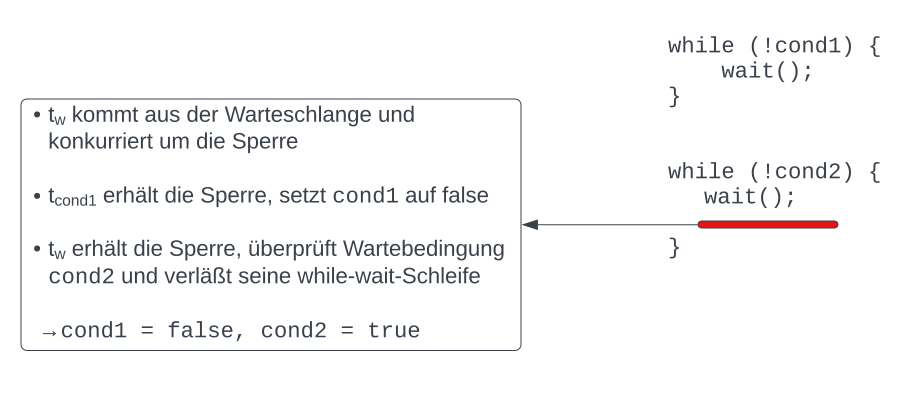
\includegraphics[scale=0.4]{chapters/Anhang/Klausuren/img/cond1cond2}
    \caption{in den rot markierten Bereich konkurriert $t_w$ um die Sperre des Objektes - wenn durch einen anderen Thread, der vor $t_w$ die Sperre erhält, \textit{cond1} auf \textit{false} gesetzt wird, stimmt die Ausgabe nicht mit der erwarteten überein. (Quelle: eigene)}
    \label{fig:cond1cond2}
\end{figure}

\noindent
Die korrekte Wartebedingung sollte lauten:

\begin{minted}[mathescape,
    linenos,
    numbersep=5pt,
    gobble=2,
    fontsize=\small,
    frame=lines,
    framesep=2mm]{java}
    public synchronized void cond1AndCond2() {
        while(!cond1 || !cond2) {
            try {
                wait();
            } catch(InterruptedException e) { }
        }
        System.out.println("cond1 and cond2:" + cond1 + " " + cond2);
    }
\end{minted}\\

Darüber hinaus müßte \code{notifyAll()} nur aufgerufen werden, wenn sowohl \code{cond1} als auch \code{cond2} auf \code{true} gesetzt sind, was leicht in den entsprechenden Methoden überprüft werden kann.
    \chapter{SS19}\label{ch:klausurss19}

\section{Aufgabe 1}

Bei der Aufgabe ist es wichtig, die Anforderungen genau zu beachten.\\
Ob eine Thread die while-wait-Schleife verlassen darf, wird von der Methode \code{tick()} gesteuert - wieviele Ticks ein Thread in der Schleife bleiben soll, wird von dem jeweiligen Thread definiert.\\
Die \code{tick()}-Methode wird von anderen Threads aufgerufen, es kann also durchaus vorkommen, dass mehrmals hintereinander
die \code{notifyAll()}-Methode aufgerufen wird - diese entfernt alle Threads aus der Warteschlange, damit die Threads ihre
Wartebedingungen erneut überprüfen können.\\
da \code{tick()} aber auch gleichzeitig einen Zähler realisieren soll, \textit{muss} es in der Methode auch eine Zählvariable geben, anhand derer die in der while-wait-Schleife enthaltenen Threads feststellen können, wie oft \code{tick()} aufgerufen wurde, um entsprechend aus der Schleife und nachfolgend der Methode herauszukommen.

\begin{figure}
    \centering
    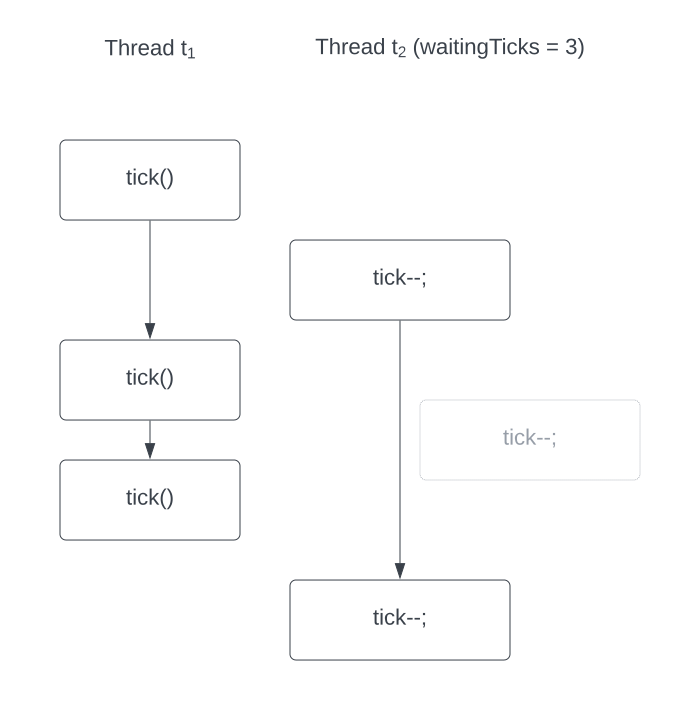
\includegraphics[scale=0.5]{chapters/Anhang/Klausuren/img/tick}
    \caption{Thread $t_1$ ruft 3 mal \texit{tick()} auf. Den Anforderungen nach müsste Thread $t_2$ danach aus der while-wait-Schleife herauskommen, erhält aber nicht die Sperre auf das Objekt von LogicalTime, um seinen eigenen Zähler rechtzeitig zu erniedrigen, bevor $t_1$ erneut \textit{tick()} aufruft. (Quelle: eigene)}
    \label{fig:tick}
\end{figure}

\section{Aufgabe 6}
Auch hier gilt, dass die Aufgabenstellung aufmerksam zu lesen ist.\\
Der Kreis soll erst ausgefüllt werden, wenn die Maustaste gelöst wird.

\begin{minted}[mathescape,
    linenos,
    numbersep=5pt,
    gobble=2,
    frame=lines,
    framesep=2mm]{java}
    private void mousePressed(double x, double y) {
        c = new Circle();
        c.setCenterX(x);
        c.setCenterY(y);
        c.setStroke(Color.RED);
        c.setFill(null); // oder Color.TRANSPARENT
        c.setRadius(RADIUS);
        graphicsPane.getChildren().add(c);
    }

    private void mouseReleased() {
        c.setFill(Color.RED);
        c = null;
    }
\end{minted}

\section{Aufgabe 8}

In der Abbildung \ref{fig:batchmodus} ist links der sequentielle Modus dargestellt, bei dem nach dem Senden einer Nachricht auf die Antwort des Servers gewartet wird, bevor eine neue Nachricht geschickt wird.
Dies wird i.d.R. verwendet, wenn das Senden einer neuen Nachricht abhängig ist von einem Ergebnis, die über die Server-Antwort übermittelt wird, oder wenn mit dem Server interagiert wird (Request abhängig vom Response).\\
Der Batch-Modus auf der rechten Seite der gleichen Abbildung ist schneller, da zwischen dem Senden von Nachrichten nicht auf Antworten gewartet werden müssen. \\
Erst nach dem Senden eine Batches von Nachrichten werden die dem Client zur Verfügung stehenden Antworten ausgelesen.\\

\noindent
In dieser Form des Batch-Modus besteht allerdings die Gefahr, dass es zu Verklemmungen kommt:
\begin{itemize}
    \item Bei dem Client kommen viele Nachrichten an, während er noch sendet.
    \item Die ankommenden Nachrichten für den Client werden gepuffert, bis sie ausgelesen werden (TCP- / OS-seitig).
    \item Läuft der Puffer voll, sorgt die Flusskontrolle (TCP) dafür, dass dem Sender mitgeteilt wird, dass keine Nachrichten mehr empfangen werden können, der Server sendet nicht mehr.
    \item Die zu sendenden Nachrichten des Servers werden in einen Puffer geschrieben.
    \item Der Sende-Puffer des Senders läuft voll.
    \item Bei dem nächsten Sende-Aufruf blockiert der Server, empfangene Nachrichten landen im Empfangspuffer
    \item Der Empfangspuffer des Servers läuft voll, der Client buffert die zu sendenden Nachrichten.
    \item Beide Anwendungen blockieren.
\end{itemize}

\\noindent
Um dieses Problem beim Batch-Modus zu umgehen, werden für das Senden und Empfangen zwei Threads auf Client-Seite erstellt: Ein Thread sendet, ein Thread empfängt. \\
Dadurch kann von dem Client immer wieder sein Empfangspuffer geleert werden, der Server wird beim Senden nicht blockiert.

\begin{figure}
    \centering
    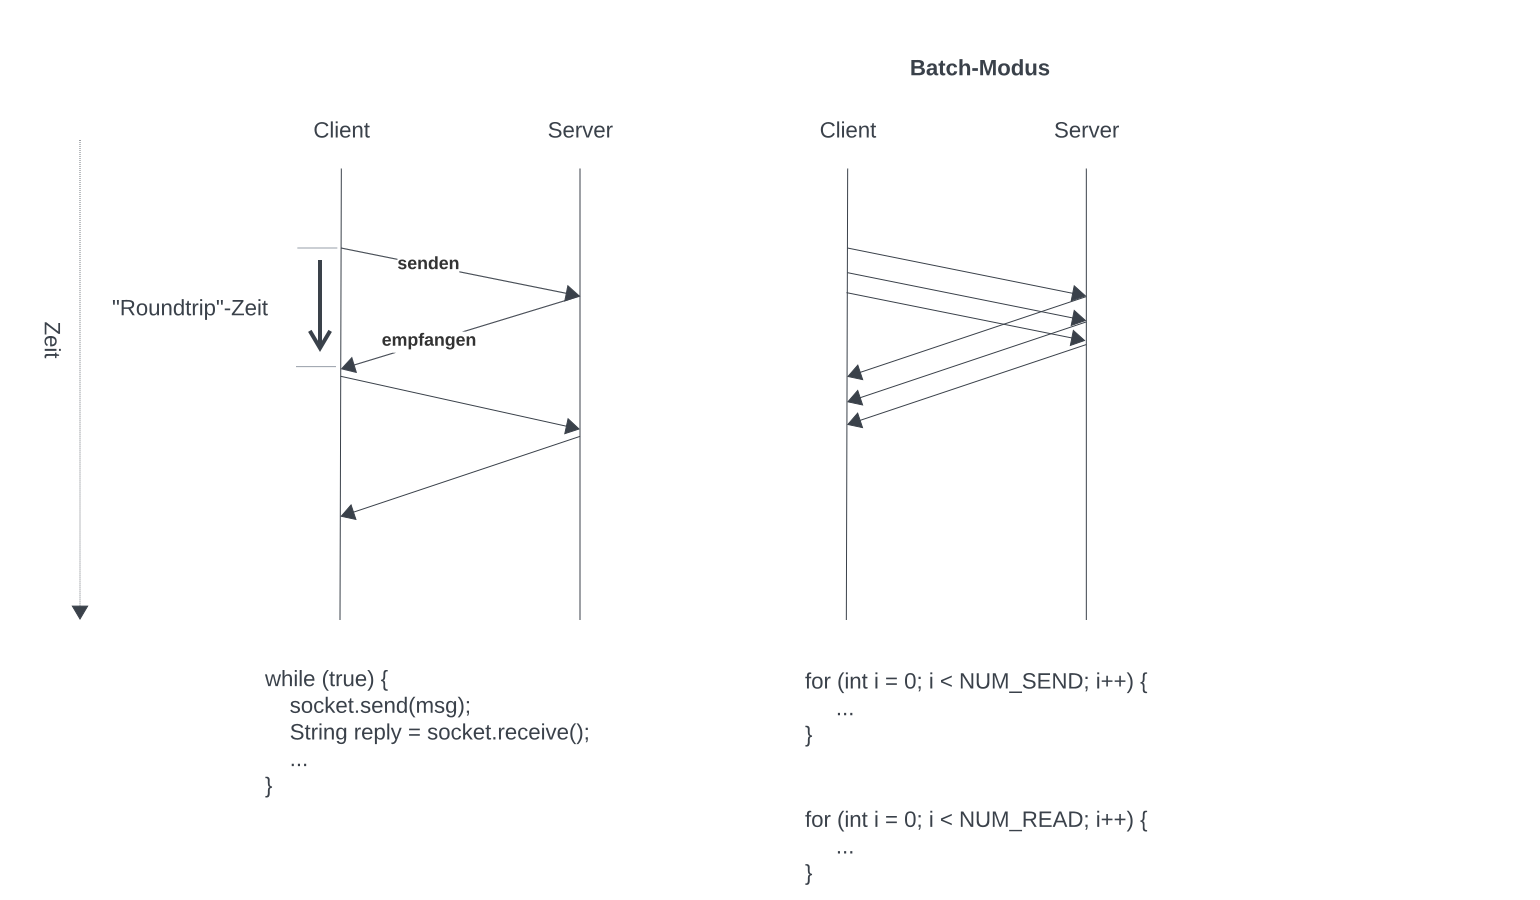
\includegraphics[scale=0.4]{chapters/Anhang/Klausuren/img/batchmodus}
    \caption{Vereinfachte Darstellung sequentieller Kommunikation und Batch-Modus (Quelle: eigene)}
    \label{fig:batchmodus}
\end{figure}
    
\begin{appendices}
    \input{chapters/Anhang/Zusatzaufgaben/index}
    \input{chapters/Anhang/Klausuren/ws13}
    \input{chapters/Anhang/Klausuren/ws15-16}
    \input{chapters/Anhang/Klausuren/ws16-17}
    \input{chapters/Anhang/Klausuren/ss19}
    \input{chapters/Anhang/Präsenzphase/index}

\end{appendices}


\end{appendices}

    \chapter{WS13}\label{ch:klausurws13}

\section{Aufgabe 1}
\subsection{Lösungsvorschlag}


\begin{minted}[mathescape,
    linenos,
    numbersep=5pt,
    gobble=2,
    fontsize=\small,
    frame=lines,
    framesep=2mm]{java}
    class Zahlenschloss {

        private int[] kombination;

        private int[] state;

        private boolean opened = false;

        public Zahlenschloss(int[] kombination) {
            this.kombination = kombination;
            this.state = new int[kombination.length];
        }

        public int anzahlRaedchen() {
            return kombination.length;
        }

        public synchronized int lesen(int radnummer) {
            return state[radnummer];
        }

        public synchronized void drehen(int radnummer, int zahl) {

            state[radnummer] = zahl;
            opened = true;
            for (int i = 0; i < anzahlRaedchen(); i++) {
                if (lesen(i) != kombination[i]) {
                    opened = false;
                    break;
                }
            }

            if (opened) {
                this.notify();
            }
        }

        public synchronized void warten() {

            while (!opened) {
                try {
                    this.wait();
                } catch (InterruptedException ignored) {}
            }
        }
    }
\end{minted}\\


\subsection{Anmerkung und Ergänzungen}

\begin{itemize}
    \item Es wird eine Wartebedingung benötigt, und zwar für die Methode \code{warten()}; ankommende Threads werden
    in die Warteschlange des Zahlenschloss-Objektes geschickt, wenn \code{opened} auf false gesetzt ist, ansonsten
    verlassen diese direkt die Methode wieder.\\
    Die Methode \code{drehen} benötigt keine separate Wartebedingung.
    Es reicht aus, sicherzustellen, dass das Zahlenschloss nicht gleichzeitig von anderen Threads benutzt werden kann:
    Die Methode \code{drehen} ist hierfür synchronisiert, damit das Zahlenschloss {insg.} immer nur eine Zustandsänderung
    erfährt - es sind andere Implementierungen möglich, in denen das Zahlenschloss dann von mehreren Threads gleichzeitig
    genutzt werden darf, wenn sich die Zugriffe anhand der ``Ziel``-\code{radnummer} unterscheiden, {bspw.} durch Mutex-Semaphore,
    die pro Radnummer verwendet werden\footnote{
        der gleichzeitige Zugriff auf unterschiedliche Arrays-Indizes ist erlaubt, s. `´17.4.1. Shared Variables``: \url{https://docs.oracle.com/javase/specs/jls/se21/html/jls-17.html#jls-1.4.1} - abgerufen 14.2.2024
    }.
    \item Es gibt nur eine Wartebedingung, von daher sollte \code{notify()} genügen.\\
    Wenn wir allerdings davon ausgehen, dass mehrere Threads über die Methode \code{warten()} in die Warteschlange des Objektes eingereiht worden sind,  sollte \code{notifyAll()} verwendet werden (siehe hierzu auch Abschnitt \ref{subsec:notifyAll}).
    Dennoch ist nicht garantiert, dass auch alle Threads aus der Warteschlange gelangen, denn es kann sein, dass ein anderer Thread die Methode \code{drehen()} betritt, dort die
    Zahlenkombination ändert und \code{opened} wieder auf \code{false} gesetzt wird. \\
    Ein anderer Thread, der nun in  \code{warten()} an die Reihe kommt, überprüft die Wartebedingung, und wird wieder in die Warteschlange eingereiht.
    Es ist also durchaus möglich, dass ein Thread nicht mehr aus der Methode \code{warten()} herauskommt.\\
    Dies könnte bspw. dadurch verhindert werden, dass die Threads in eine Queue gepackt werden, und in \code{drehen()} eine Wartebedingung eingefügt wird, die erst erfüllt ist,
    wenn die Queue geleert wurde oder aus ihr entnommen wurde, in der Reihenfolge, in der die Threads in die Queue eingereiht worden sind (\textit{FIFO}) (s. a. Abschnitt~\ref{subsec:readerwriterproblem}).
    \item Bei der Teilaufgabe mit der Schleife muss die komplette Schleife synchronisiert werden, was man durch ein \code{synchronized}-Statement erreicht\footnote{siehe Abschnitt~\ref{subsec:synchronizedstatement}.}
    \begin{minted}[mathescape,
        linenos,
        numbersep=5pt,
        gobble=2,
        fontsize=\small,
        frame=lines,
        framesep=2mm]{java}
        synchronized (zk) {
            for (int i = 0; i < anzahlRaedchen; i++) {
                System.out.println(zk.lesen(i));
            }
        }
    \end{minted}
    Ansonsten läuft man Gefahr, dass sich nach Auslesen der 1. Position der Wert von Position 2 geändert hat und dadurch eine
    Zahlenkombination ausgegeben wird, die es nicht gegeben hat:
    \begin{enumerate}
        \item $K\coloneqq[0, 0, 0]$
        \item Position $K_0$ wird ausgelesen und liefert $0$.
        \item Thread ändert $K_0$ zu $1$ $\implies K\coloneqq[1, 0, 0] $.
        \item Thread ändert $K_1$ zu $2$ $\implies K\coloneqq[1, 2, 0] $.
        \item Thread ändert $K_2$ zu $3$ $\implies K\coloneqq[1, 2, 3] $.
        \item Positionen $K_1$ und $K_2$ werden ausgelesen und liefern: $2, 3$
        \item Ausgabe: $0, 2, 3$ - diese Kombination hat es in dem Fall aber tatsächlich nicht gegeben.
    \end{enumerate}
\end{itemize}

\begin{tcolorbox}[colback=red!20,color=white,title=Anmerkung]
    Die Methode \code{lesen()} als \code{synchronized} zu markieren könnte man sich vlt. sparen, wenn man davon ausgeht,
    dass die Methode ohnehin in einem \code{synchronized}-Statement verwendet wird, um alle Rädchen abzulesen.\\
    Mehrere Threads können also nicht parallel auf unterschiedliche Positionen des Feldes zugreifen, wenn die Methode
    synchronisiert ist.\\
    Allerdings ist sowohl das Skript als auch das Buch recht klar, was in dieser Situation geschehen muss (s. Skript Fopt1/2, S. 9, außerdem \cite[31, Abschnitt 2.3.6]{Oec22}): Es muss (in diesem Kurs) immer \code{synchronized} verwendet werden, wenn gleichzeitig
    Daten geschrieben und gleichzeitig diese Daten gelesen werden sollen - und eine andere Implementierung, bei der die
    einzelnen Positionen ``gelocked`` sind, so dass ein gleichzeitiger Zugriff auf unterschiedliche Rädchen möglich ist, war nicht gefordert.\\
    Ggfl. würde in anderen Implementierungen der Einsatz von \code{AtomicReferenceArray}\footnote{s. \cite[157 ff.]{Oec22}
    s. ``Class AtomicReferenceArray<E>``: \url{https://docs.oracle.com/en/java/javase/21/docs/api/java.base/java/util/concurrent/atomic/AtomicReferenceArray.html} - abgerufen 15.2.2024
    } Sinn machen, aber das Lehrmaterial ist bereits sehr eindeutig bzgl. der Verwendung von \code{synchronized}.
\end{tcolorbox}



\section{Aufgabe 3}
\subsection{Lösungsvorschlag}

\subsection*{Statische Parallelität}
Statische Parallelität erlaubt es einem Server, eine \textit{fixe} Anzahl von Verbindungen gleichzeitig zu bedienen.\\
Hierbei wird ein Feld von Threads erstellt, wobei jeder Thread das \code{ServerSocket}-Objekt als Referenz übergeben bekommt.
In der \code{run()}-Methode wird dann über \code{accept()} in einer Endlosschleife auf eingehende Verbindungen gewartet, die dann so lange bedient werden, bis sich ein Client wieder abmeldet (oder eine andere Abbruchbedingung erfüllt ist, wie z.B. ein \code{SocketTimeout}).\\
Das sich ein Client abmeldet, bekommt man bspw. dadurch mit, dass \code{null} beim Lesen von einer Nachricht des Clients zurückgegeben wird (vgl. \cite[286]{Oec22}. \\
Siehe Abschnitt~\ref{sec:seqparserver} für ein Implementierungsbeispiel.



\subsection*{Dynamische Parallelität}

Bei der \textbf{Dynamischer Parallelität} erzeugt der Server für jede Verbindung einen neuen Thread, der so lange läuft, bis der Client die Verbindung wieder trennt.\\
Die Anzahl der Threads ändert sich dadurch laufend.\\
Wird die max. Anzahl erlaubter Threads nicht kontrolliert, kann es zu einer Überlastung des Server-Rechners kommen (bspw. durch einen Denial-of-Service-Angriff.)\\

\noindent
I.d.R. ist eine Mischform aus beidem geeignet, um mehrere Clients gleichzeitig bedienen zu können, und dabei nicht Gefahr zu laufen, durch dynamisches, unbegrenztes Wachstum der Anzahl der Threads überlastet zu werden.

    \chapter{WS13}\label{ch:klausurws5-16}

\section{Rechteck-Scroll (SS15 Aufgabe 2)}

Aufgabenstellung unklar.\\
Mögliche Implementierung unter \url{https://github.com/ThorstenSuckow/fopt/tree/main/src/main/java/klausurvorbereitung/foptws1516/MouseDragsSquareDemo}.

\section{Rechteck-Scroll (WS15/16 Aufgabe 1)}

Aufgabenstellung unklar.\\
Mögliche Implementierung unter \url{https://github.com/ThorstenSuckow/fopt/tree/main/src/main/java/klausurvorbereitung/foptws1516/MaxWeightDemo}.\\

\noindent
Es gibt nur eine Warteschlange für Threads in \code{use()}, es gibt keine Wartebedingung in \code{dontUse()} und damit auch keine weitere Warteschlange.\\
Es sind durch die Zugriffe auf unterschiedliche Indizes allerdings mehrere Wartebedingungen vorhanden, weshalb hab \code{notifyAll()} nutzen sollte,
sobald ein Zugriff auf ein Feld nach Aufruf von \code{dontUse} wieder möglich wird.\\
Ansonsten bestünde die Gefahr, dass bei dem Einsatz von \code{notify()} ein wartender Thread nicht geweckt wird, obwohl er weiterlaufen könnte:\\
Angenommen, das Feld $F$ hat eine Länge von $3$, das \code{maxWeight} ist mit $2$ konfiguriert.
Thread $t_1$ mit einer Laufzeit von $200\ sek$ bekommt Zugriff auf $F_0$, setzt $currentWeight$ auf $1$.\\
Thread $t_2$ mit einer Laufzeit von $1\ sek$ möchte auf $F_1$ zugreifen, setzt $currentWeight=2$ in die Warteschlange.\\
Thread $t_3$ meldet Zugriff auf $F_0$ an und gelangt in die Warteschlange.\\
Thread $t_4$ meldet Zugriff auf $F_1$ an und gelangt in die Warteschlange.\\
Thread $t_2$ ist mit der Bearbeitung von $F_1$ fertig, $currentWeight$ wird auf $1$ gesetzt, \code{notify()} wird aufgerufen.\\
Thread $t_3$ wird aus der Warteschlange geholt, kann aber nicht weiterarbeiten, da $F_0$ noch durch den länger dauernden $t_1$ blockiert ist, und kommt wieder in die Warteschlange.\\

\noindent
Offensichtlich hätte in dem Beispiel \code{notifyAll()} dazu geführt, dass auch $T_4$ seine Wartebedingung hätte überprüfen können, und hätte so Zugriff auf $F_1$ bekommen.
Stattdessen muss nun gewartet werden, bis das nächste \code{notify()} aufgerufen wird, oder ein neu ankommender Thread $F_1$ belegt.

    \chapter{WS16-17}\label{ch:klausurws16-17}

\section{Aufgabe 1}
\subsection{Lösungshinweis}

Die erste Aufgabe verdeutlicht, was bei einem \code{notifyAll()} und unsauber gesetzten Wartebedingungen passieren kann.\\
Sei folgender Quellcode gegeben:


\begin{minted}[mathescape,
    linenos,
    numbersep=5pt,
    gobble=2,
    fontsize=\small,
    frame=lines,
    framesep=2mm]{java}
    class Cond1AndCond2 {

        private boolean cond1;
        private boolean cond2;

        public synchronized void setCond1(boolean c) {
            cond1 = c;
            notifyAll();
        }

        public synchronized void setCond2(boolean c) {
            cond2 = c;
            notifyAll();
        }

        public synchronized void cond1AndCond2() {
            while(!cond1) {
                try {
                    wait();
                } catch(InterruptedException e) { }
            }

            while(!cond2) {
                try {
                    wait();
                } catch(InterruptedException e) {}
            }
            System.out.println("cond1 and cond2:" + cond1 + " " + cond2);
        }
    }
\end{minted}\\

Man sollte auf den ersten Blick meinen, dass \code{cond1} und \code{cond2} beide \code{true} sein müssen, damit die Ausgabe erfolgt.\\
Tatsächlich ist es aber so, dass es in der Methode zwei unterschiedliche Wartebedingungen gibt.\\
Die erste Wartebedingung schickt einen Thread in die Warteschlange, wenn \code{cond1 == false} gilt.\\
Setzt ein anderer Thread über \code{setCond1(true)} das Attribut entsprechend auf \code{true}, bewirkt der nachfolgende Aufruf von \code{notifyAll()}, dass alle \textit{wartenden} Threads aus der Warteschlange entfernt werden und erneut um eine Sperre des Objektes konkurrieren.\\
Erhält ein entsprechender Thread $t_w$ die Sperre auf das Objekt und kann seine \textit{while-wait-Schleife} verlassen, kann es vorkommen, dass er erneut in die Warteschlange eingereiht wird, wegen der nachfolgenden Wartebedingung \code{cond2 == false}.\\
Angenommen, ein weiterer Thread ruft nun \code{setCond2(true)} auf, und $t_w$ kommt aus der Warteschlange und konkurriert erneut und um die Sperre des Objektes, dann kann es vorkommen, das ein anderer Thread zunächst die Sperre erhält, \code{cond1} wieder auf \code{false} setzt, dann erhält $t_w$ die Sperre, überprüft die Wartebedingung \code{cond2 == false}.\\
Wegen \code{cond2} gelangt er aus der \textit{while-wait-Schleife} und die Ausgabe erfolgt - da zwischenzeitlich \code{cond1} wieder auf \code{false} gesetzt wurde, ist die erwartete Ausgabe nicht \code{true true}, sondern \code{false true} (s. Abbildung \ref{fig:cond1cond2}).\\

\begin{figure}
    \centering
    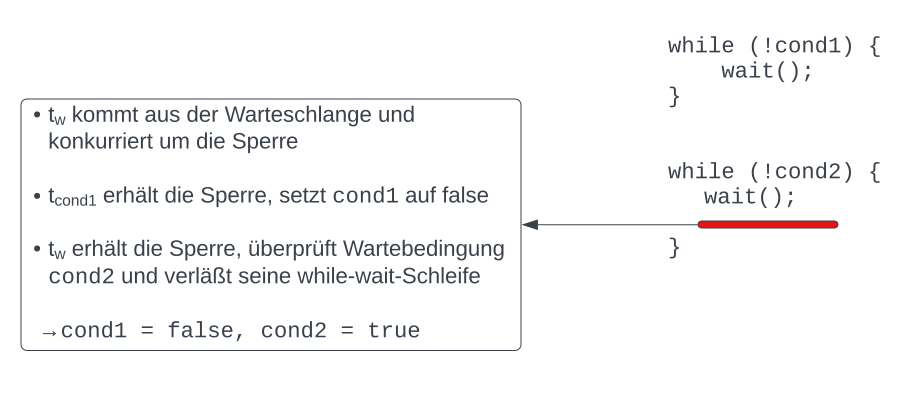
\includegraphics[scale=0.4]{chapters/Anhang/Klausuren/img/cond1cond2}
    \caption{in den rot markierten Bereich konkurriert $t_w$ um die Sperre des Objektes - wenn durch einen anderen Thread, der vor $t_w$ die Sperre erhält, \textit{cond1} auf \textit{false} gesetzt wird, stimmt die Ausgabe nicht mit der erwarteten überein. (Quelle: eigene)}
    \label{fig:cond1cond2}
\end{figure}

\noindent
Die korrekte Wartebedingung sollte lauten:

\begin{minted}[mathescape,
    linenos,
    numbersep=5pt,
    gobble=2,
    fontsize=\small,
    frame=lines,
    framesep=2mm]{java}
    public synchronized void cond1AndCond2() {
        while(!cond1 || !cond2) {
            try {
                wait();
            } catch(InterruptedException e) { }
        }
        System.out.println("cond1 and cond2:" + cond1 + " " + cond2);
    }
\end{minted}\\

Darüber hinaus müßte \code{notifyAll()} nur aufgerufen werden, wenn sowohl \code{cond1} als auch \code{cond2} auf \code{true} gesetzt sind, was leicht in den entsprechenden Methoden überprüft werden kann.
    \chapter{SS19}\label{ch:klausurss19}

\section{Aufgabe 1}

Bei der Aufgabe ist es wichtig, die Anforderungen genau zu beachten.\\
Ob eine Thread die while-wait-Schleife verlassen darf, wird von der Methode \code{tick()} gesteuert - wieviele Ticks ein Thread in der Schleife bleiben soll, wird von dem jeweiligen Thread definiert.\\
Die \code{tick()}-Methode wird von anderen Threads aufgerufen, es kann also durchaus vorkommen, dass mehrmals hintereinander
die \code{notifyAll()}-Methode aufgerufen wird - diese entfernt alle Threads aus der Warteschlange, damit die Threads ihre
Wartebedingungen erneut überprüfen können.\\
da \code{tick()} aber auch gleichzeitig einen Zähler realisieren soll, \textit{muss} es in der Methode auch eine Zählvariable geben, anhand derer die in der while-wait-Schleife enthaltenen Threads feststellen können, wie oft \code{tick()} aufgerufen wurde, um entsprechend aus der Schleife und nachfolgend der Methode herauszukommen.

\begin{figure}
    \centering
    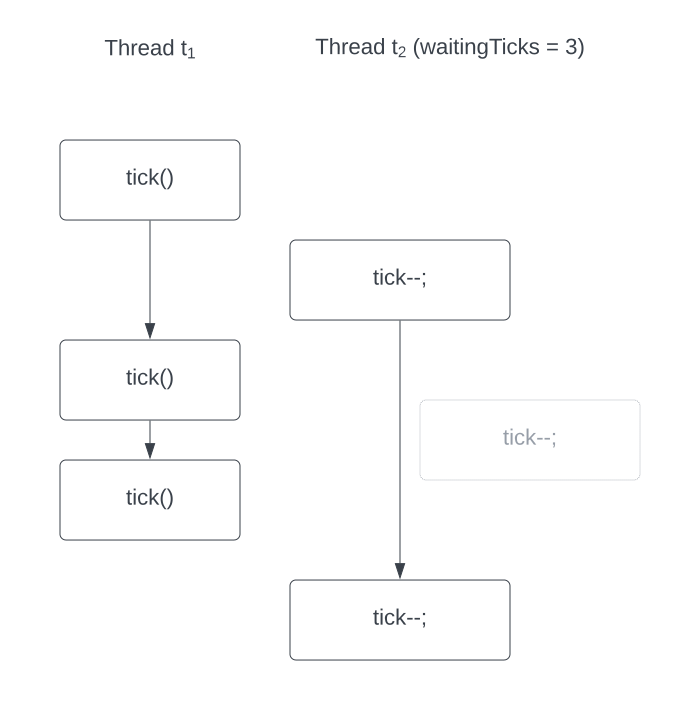
\includegraphics[scale=0.5]{chapters/Anhang/Klausuren/img/tick}
    \caption{Thread $t_1$ ruft 3 mal \texit{tick()} auf. Den Anforderungen nach müsste Thread $t_2$ danach aus der while-wait-Schleife herauskommen, erhält aber nicht die Sperre auf das Objekt von LogicalTime, um seinen eigenen Zähler rechtzeitig zu erniedrigen, bevor $t_1$ erneut \textit{tick()} aufruft. (Quelle: eigene)}
    \label{fig:tick}
\end{figure}

\section{Aufgabe 6}
Auch hier gilt, dass die Aufgabenstellung aufmerksam zu lesen ist.\\
Der Kreis soll erst ausgefüllt werden, wenn die Maustaste gelöst wird.

\begin{minted}[mathescape,
    linenos,
    numbersep=5pt,
    gobble=2,
    frame=lines,
    framesep=2mm]{java}
    private void mousePressed(double x, double y) {
        c = new Circle();
        c.setCenterX(x);
        c.setCenterY(y);
        c.setStroke(Color.RED);
        c.setFill(null); // oder Color.TRANSPARENT
        c.setRadius(RADIUS);
        graphicsPane.getChildren().add(c);
    }

    private void mouseReleased() {
        c.setFill(Color.RED);
        c = null;
    }
\end{minted}

\section{Aufgabe 8}

In der Abbildung \ref{fig:batchmodus} ist links der sequentielle Modus dargestellt, bei dem nach dem Senden einer Nachricht auf die Antwort des Servers gewartet wird, bevor eine neue Nachricht geschickt wird.
Dies wird i.d.R. verwendet, wenn das Senden einer neuen Nachricht abhängig ist von einem Ergebnis, die über die Server-Antwort übermittelt wird, oder wenn mit dem Server interagiert wird (Request abhängig vom Response).\\
Der Batch-Modus auf der rechten Seite der gleichen Abbildung ist schneller, da zwischen dem Senden von Nachrichten nicht auf Antworten gewartet werden müssen. \\
Erst nach dem Senden eine Batches von Nachrichten werden die dem Client zur Verfügung stehenden Antworten ausgelesen.\\

\noindent
In dieser Form des Batch-Modus besteht allerdings die Gefahr, dass es zu Verklemmungen kommt:
\begin{itemize}
    \item Bei dem Client kommen viele Nachrichten an, während er noch sendet.
    \item Die ankommenden Nachrichten für den Client werden gepuffert, bis sie ausgelesen werden (TCP- / OS-seitig).
    \item Läuft der Puffer voll, sorgt die Flusskontrolle (TCP) dafür, dass dem Sender mitgeteilt wird, dass keine Nachrichten mehr empfangen werden können, der Server sendet nicht mehr.
    \item Die zu sendenden Nachrichten des Servers werden in einen Puffer geschrieben.
    \item Der Sende-Puffer des Senders läuft voll.
    \item Bei dem nächsten Sende-Aufruf blockiert der Server, empfangene Nachrichten landen im Empfangspuffer
    \item Der Empfangspuffer des Servers läuft voll, der Client buffert die zu sendenden Nachrichten.
    \item Beide Anwendungen blockieren.
\end{itemize}

\\noindent
Um dieses Problem beim Batch-Modus zu umgehen, werden für das Senden und Empfangen zwei Threads auf Client-Seite erstellt: Ein Thread sendet, ein Thread empfängt. \\
Dadurch kann von dem Client immer wieder sein Empfangspuffer geleert werden, der Server wird beim Senden nicht blockiert.

\begin{figure}
    \centering
    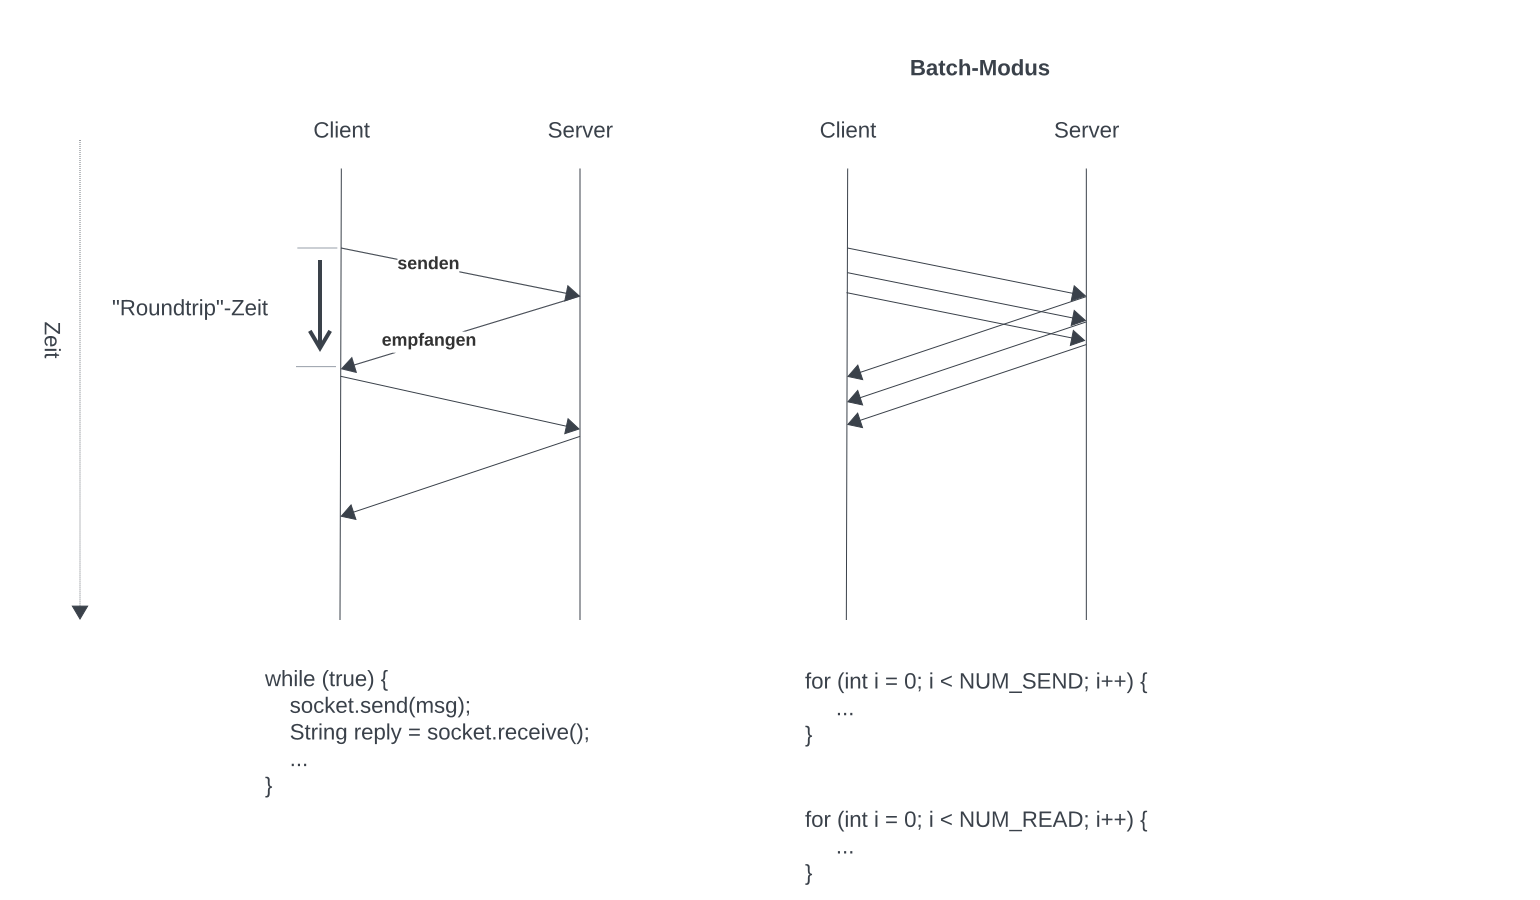
\includegraphics[scale=0.4]{chapters/Anhang/Klausuren/img/batchmodus}
    \caption{Vereinfachte Darstellung sequentieller Kommunikation und Batch-Modus (Quelle: eigene)}
    \label{fig:batchmodus}
\end{figure}
    
\begin{appendices}
    
\begin{appendices}
    \input{chapters/Anhang/Zusatzaufgaben/index}
    \input{chapters/Anhang/Klausuren/ws13}
    \input{chapters/Anhang/Klausuren/ws15-16}
    \input{chapters/Anhang/Klausuren/ws16-17}
    \input{chapters/Anhang/Klausuren/ss19}
    \input{chapters/Anhang/Präsenzphase/index}

\end{appendices}

    \chapter{WS13}\label{ch:klausurws13}

\section{Aufgabe 1}
\subsection{Lösungsvorschlag}


\begin{minted}[mathescape,
    linenos,
    numbersep=5pt,
    gobble=2,
    fontsize=\small,
    frame=lines,
    framesep=2mm]{java}
    class Zahlenschloss {

        private int[] kombination;

        private int[] state;

        private boolean opened = false;

        public Zahlenschloss(int[] kombination) {
            this.kombination = kombination;
            this.state = new int[kombination.length];
        }

        public int anzahlRaedchen() {
            return kombination.length;
        }

        public synchronized int lesen(int radnummer) {
            return state[radnummer];
        }

        public synchronized void drehen(int radnummer, int zahl) {

            state[radnummer] = zahl;
            opened = true;
            for (int i = 0; i < anzahlRaedchen(); i++) {
                if (lesen(i) != kombination[i]) {
                    opened = false;
                    break;
                }
            }

            if (opened) {
                this.notify();
            }
        }

        public synchronized void warten() {

            while (!opened) {
                try {
                    this.wait();
                } catch (InterruptedException ignored) {}
            }
        }
    }
\end{minted}\\


\subsection{Anmerkung und Ergänzungen}

\begin{itemize}
    \item Es wird eine Wartebedingung benötigt, und zwar für die Methode \code{warten()}; ankommende Threads werden
    in die Warteschlange des Zahlenschloss-Objektes geschickt, wenn \code{opened} auf false gesetzt ist, ansonsten
    verlassen diese direkt die Methode wieder.\\
    Die Methode \code{drehen} benötigt keine separate Wartebedingung.
    Es reicht aus, sicherzustellen, dass das Zahlenschloss nicht gleichzeitig von anderen Threads benutzt werden kann:
    Die Methode \code{drehen} ist hierfür synchronisiert, damit das Zahlenschloss {insg.} immer nur eine Zustandsänderung
    erfährt - es sind andere Implementierungen möglich, in denen das Zahlenschloss dann von mehreren Threads gleichzeitig
    genutzt werden darf, wenn sich die Zugriffe anhand der ``Ziel``-\code{radnummer} unterscheiden, {bspw.} durch Mutex-Semaphore,
    die pro Radnummer verwendet werden\footnote{
        der gleichzeitige Zugriff auf unterschiedliche Arrays-Indizes ist erlaubt, s. `´17.4.1. Shared Variables``: \url{https://docs.oracle.com/javase/specs/jls/se21/html/jls-17.html#jls-1.4.1} - abgerufen 14.2.2024
    }.
    \item Es gibt nur eine Wartebedingung, von daher sollte \code{notify()} genügen.\\
    Wenn wir allerdings davon ausgehen, dass mehrere Threads über die Methode \code{warten()} in die Warteschlange des Objektes eingereiht worden sind,  sollte \code{notifyAll()} verwendet werden (siehe hierzu auch Abschnitt \ref{subsec:notifyAll}).
    Dennoch ist nicht garantiert, dass auch alle Threads aus der Warteschlange gelangen, denn es kann sein, dass ein anderer Thread die Methode \code{drehen()} betritt, dort die
    Zahlenkombination ändert und \code{opened} wieder auf \code{false} gesetzt wird. \\
    Ein anderer Thread, der nun in  \code{warten()} an die Reihe kommt, überprüft die Wartebedingung, und wird wieder in die Warteschlange eingereiht.
    Es ist also durchaus möglich, dass ein Thread nicht mehr aus der Methode \code{warten()} herauskommt.\\
    Dies könnte bspw. dadurch verhindert werden, dass die Threads in eine Queue gepackt werden, und in \code{drehen()} eine Wartebedingung eingefügt wird, die erst erfüllt ist,
    wenn die Queue geleert wurde oder aus ihr entnommen wurde, in der Reihenfolge, in der die Threads in die Queue eingereiht worden sind (\textit{FIFO}) (s. a. Abschnitt~\ref{subsec:readerwriterproblem}).
    \item Bei der Teilaufgabe mit der Schleife muss die komplette Schleife synchronisiert werden, was man durch ein \code{synchronized}-Statement erreicht\footnote{siehe Abschnitt~\ref{subsec:synchronizedstatement}.}
    \begin{minted}[mathescape,
        linenos,
        numbersep=5pt,
        gobble=2,
        fontsize=\small,
        frame=lines,
        framesep=2mm]{java}
        synchronized (zk) {
            for (int i = 0; i < anzahlRaedchen; i++) {
                System.out.println(zk.lesen(i));
            }
        }
    \end{minted}
    Ansonsten läuft man Gefahr, dass sich nach Auslesen der 1. Position der Wert von Position 2 geändert hat und dadurch eine
    Zahlenkombination ausgegeben wird, die es nicht gegeben hat:
    \begin{enumerate}
        \item $K\coloneqq[0, 0, 0]$
        \item Position $K_0$ wird ausgelesen und liefert $0$.
        \item Thread ändert $K_0$ zu $1$ $\implies K\coloneqq[1, 0, 0] $.
        \item Thread ändert $K_1$ zu $2$ $\implies K\coloneqq[1, 2, 0] $.
        \item Thread ändert $K_2$ zu $3$ $\implies K\coloneqq[1, 2, 3] $.
        \item Positionen $K_1$ und $K_2$ werden ausgelesen und liefern: $2, 3$
        \item Ausgabe: $0, 2, 3$ - diese Kombination hat es in dem Fall aber tatsächlich nicht gegeben.
    \end{enumerate}
\end{itemize}

\begin{tcolorbox}[colback=red!20,color=white,title=Anmerkung]
    Die Methode \code{lesen()} als \code{synchronized} zu markieren könnte man sich vlt. sparen, wenn man davon ausgeht,
    dass die Methode ohnehin in einem \code{synchronized}-Statement verwendet wird, um alle Rädchen abzulesen.\\
    Mehrere Threads können also nicht parallel auf unterschiedliche Positionen des Feldes zugreifen, wenn die Methode
    synchronisiert ist.\\
    Allerdings ist sowohl das Skript als auch das Buch recht klar, was in dieser Situation geschehen muss (s. Skript Fopt1/2, S. 9, außerdem \cite[31, Abschnitt 2.3.6]{Oec22}): Es muss (in diesem Kurs) immer \code{synchronized} verwendet werden, wenn gleichzeitig
    Daten geschrieben und gleichzeitig diese Daten gelesen werden sollen - und eine andere Implementierung, bei der die
    einzelnen Positionen ``gelocked`` sind, so dass ein gleichzeitiger Zugriff auf unterschiedliche Rädchen möglich ist, war nicht gefordert.\\
    Ggfl. würde in anderen Implementierungen der Einsatz von \code{AtomicReferenceArray}\footnote{s. \cite[157 ff.]{Oec22}
    s. ``Class AtomicReferenceArray<E>``: \url{https://docs.oracle.com/en/java/javase/21/docs/api/java.base/java/util/concurrent/atomic/AtomicReferenceArray.html} - abgerufen 15.2.2024
    } Sinn machen, aber das Lehrmaterial ist bereits sehr eindeutig bzgl. der Verwendung von \code{synchronized}.
\end{tcolorbox}



\section{Aufgabe 3}
\subsection{Lösungsvorschlag}

\subsection*{Statische Parallelität}
Statische Parallelität erlaubt es einem Server, eine \textit{fixe} Anzahl von Verbindungen gleichzeitig zu bedienen.\\
Hierbei wird ein Feld von Threads erstellt, wobei jeder Thread das \code{ServerSocket}-Objekt als Referenz übergeben bekommt.
In der \code{run()}-Methode wird dann über \code{accept()} in einer Endlosschleife auf eingehende Verbindungen gewartet, die dann so lange bedient werden, bis sich ein Client wieder abmeldet (oder eine andere Abbruchbedingung erfüllt ist, wie z.B. ein \code{SocketTimeout}).\\
Das sich ein Client abmeldet, bekommt man bspw. dadurch mit, dass \code{null} beim Lesen von einer Nachricht des Clients zurückgegeben wird (vgl. \cite[286]{Oec22}. \\
Siehe Abschnitt~\ref{sec:seqparserver} für ein Implementierungsbeispiel.



\subsection*{Dynamische Parallelität}

Bei der \textbf{Dynamischer Parallelität} erzeugt der Server für jede Verbindung einen neuen Thread, der so lange läuft, bis der Client die Verbindung wieder trennt.\\
Die Anzahl der Threads ändert sich dadurch laufend.\\
Wird die max. Anzahl erlaubter Threads nicht kontrolliert, kann es zu einer Überlastung des Server-Rechners kommen (bspw. durch einen Denial-of-Service-Angriff.)\\

\noindent
I.d.R. ist eine Mischform aus beidem geeignet, um mehrere Clients gleichzeitig bedienen zu können, und dabei nicht Gefahr zu laufen, durch dynamisches, unbegrenztes Wachstum der Anzahl der Threads überlastet zu werden.

    \chapter{WS13}\label{ch:klausurws5-16}

\section{Rechteck-Scroll (SS15 Aufgabe 2)}

Aufgabenstellung unklar.\\
Mögliche Implementierung unter \url{https://github.com/ThorstenSuckow/fopt/tree/main/src/main/java/klausurvorbereitung/foptws1516/MouseDragsSquareDemo}.

\section{Rechteck-Scroll (WS15/16 Aufgabe 1)}

Aufgabenstellung unklar.\\
Mögliche Implementierung unter \url{https://github.com/ThorstenSuckow/fopt/tree/main/src/main/java/klausurvorbereitung/foptws1516/MaxWeightDemo}.\\

\noindent
Es gibt nur eine Warteschlange für Threads in \code{use()}, es gibt keine Wartebedingung in \code{dontUse()} und damit auch keine weitere Warteschlange.\\
Es sind durch die Zugriffe auf unterschiedliche Indizes allerdings mehrere Wartebedingungen vorhanden, weshalb hab \code{notifyAll()} nutzen sollte,
sobald ein Zugriff auf ein Feld nach Aufruf von \code{dontUse} wieder möglich wird.\\
Ansonsten bestünde die Gefahr, dass bei dem Einsatz von \code{notify()} ein wartender Thread nicht geweckt wird, obwohl er weiterlaufen könnte:\\
Angenommen, das Feld $F$ hat eine Länge von $3$, das \code{maxWeight} ist mit $2$ konfiguriert.
Thread $t_1$ mit einer Laufzeit von $200\ sek$ bekommt Zugriff auf $F_0$, setzt $currentWeight$ auf $1$.\\
Thread $t_2$ mit einer Laufzeit von $1\ sek$ möchte auf $F_1$ zugreifen, setzt $currentWeight=2$ in die Warteschlange.\\
Thread $t_3$ meldet Zugriff auf $F_0$ an und gelangt in die Warteschlange.\\
Thread $t_4$ meldet Zugriff auf $F_1$ an und gelangt in die Warteschlange.\\
Thread $t_2$ ist mit der Bearbeitung von $F_1$ fertig, $currentWeight$ wird auf $1$ gesetzt, \code{notify()} wird aufgerufen.\\
Thread $t_3$ wird aus der Warteschlange geholt, kann aber nicht weiterarbeiten, da $F_0$ noch durch den länger dauernden $t_1$ blockiert ist, und kommt wieder in die Warteschlange.\\

\noindent
Offensichtlich hätte in dem Beispiel \code{notifyAll()} dazu geführt, dass auch $T_4$ seine Wartebedingung hätte überprüfen können, und hätte so Zugriff auf $F_1$ bekommen.
Stattdessen muss nun gewartet werden, bis das nächste \code{notify()} aufgerufen wird, oder ein neu ankommender Thread $F_1$ belegt.

    \chapter{WS16-17}\label{ch:klausurws16-17}

\section{Aufgabe 1}
\subsection{Lösungshinweis}

Die erste Aufgabe verdeutlicht, was bei einem \code{notifyAll()} und unsauber gesetzten Wartebedingungen passieren kann.\\
Sei folgender Quellcode gegeben:


\begin{minted}[mathescape,
    linenos,
    numbersep=5pt,
    gobble=2,
    fontsize=\small,
    frame=lines,
    framesep=2mm]{java}
    class Cond1AndCond2 {

        private boolean cond1;
        private boolean cond2;

        public synchronized void setCond1(boolean c) {
            cond1 = c;
            notifyAll();
        }

        public synchronized void setCond2(boolean c) {
            cond2 = c;
            notifyAll();
        }

        public synchronized void cond1AndCond2() {
            while(!cond1) {
                try {
                    wait();
                } catch(InterruptedException e) { }
            }

            while(!cond2) {
                try {
                    wait();
                } catch(InterruptedException e) {}
            }
            System.out.println("cond1 and cond2:" + cond1 + " " + cond2);
        }
    }
\end{minted}\\

Man sollte auf den ersten Blick meinen, dass \code{cond1} und \code{cond2} beide \code{true} sein müssen, damit die Ausgabe erfolgt.\\
Tatsächlich ist es aber so, dass es in der Methode zwei unterschiedliche Wartebedingungen gibt.\\
Die erste Wartebedingung schickt einen Thread in die Warteschlange, wenn \code{cond1 == false} gilt.\\
Setzt ein anderer Thread über \code{setCond1(true)} das Attribut entsprechend auf \code{true}, bewirkt der nachfolgende Aufruf von \code{notifyAll()}, dass alle \textit{wartenden} Threads aus der Warteschlange entfernt werden und erneut um eine Sperre des Objektes konkurrieren.\\
Erhält ein entsprechender Thread $t_w$ die Sperre auf das Objekt und kann seine \textit{while-wait-Schleife} verlassen, kann es vorkommen, dass er erneut in die Warteschlange eingereiht wird, wegen der nachfolgenden Wartebedingung \code{cond2 == false}.\\
Angenommen, ein weiterer Thread ruft nun \code{setCond2(true)} auf, und $t_w$ kommt aus der Warteschlange und konkurriert erneut und um die Sperre des Objektes, dann kann es vorkommen, das ein anderer Thread zunächst die Sperre erhält, \code{cond1} wieder auf \code{false} setzt, dann erhält $t_w$ die Sperre, überprüft die Wartebedingung \code{cond2 == false}.\\
Wegen \code{cond2} gelangt er aus der \textit{while-wait-Schleife} und die Ausgabe erfolgt - da zwischenzeitlich \code{cond1} wieder auf \code{false} gesetzt wurde, ist die erwartete Ausgabe nicht \code{true true}, sondern \code{false true} (s. Abbildung \ref{fig:cond1cond2}).\\

\begin{figure}
    \centering
    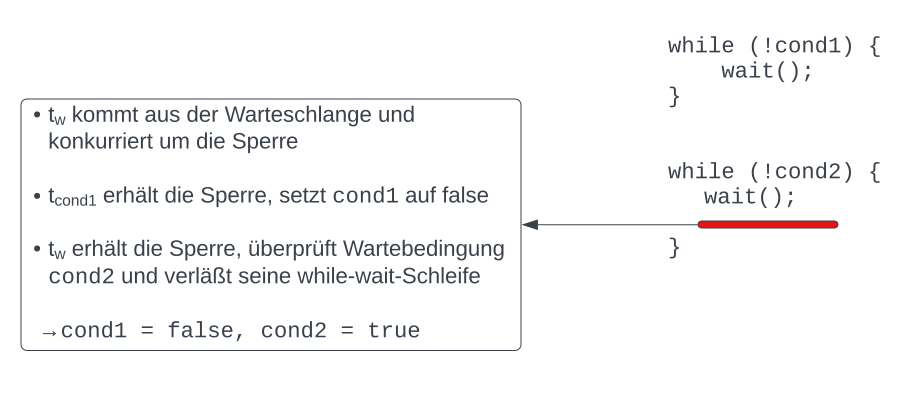
\includegraphics[scale=0.4]{chapters/Anhang/Klausuren/img/cond1cond2}
    \caption{in den rot markierten Bereich konkurriert $t_w$ um die Sperre des Objektes - wenn durch einen anderen Thread, der vor $t_w$ die Sperre erhält, \textit{cond1} auf \textit{false} gesetzt wird, stimmt die Ausgabe nicht mit der erwarteten überein. (Quelle: eigene)}
    \label{fig:cond1cond2}
\end{figure}

\noindent
Die korrekte Wartebedingung sollte lauten:

\begin{minted}[mathescape,
    linenos,
    numbersep=5pt,
    gobble=2,
    fontsize=\small,
    frame=lines,
    framesep=2mm]{java}
    public synchronized void cond1AndCond2() {
        while(!cond1 || !cond2) {
            try {
                wait();
            } catch(InterruptedException e) { }
        }
        System.out.println("cond1 and cond2:" + cond1 + " " + cond2);
    }
\end{minted}\\

Darüber hinaus müßte \code{notifyAll()} nur aufgerufen werden, wenn sowohl \code{cond1} als auch \code{cond2} auf \code{true} gesetzt sind, was leicht in den entsprechenden Methoden überprüft werden kann.
    \chapter{SS19}\label{ch:klausurss19}

\section{Aufgabe 1}

Bei der Aufgabe ist es wichtig, die Anforderungen genau zu beachten.\\
Ob eine Thread die while-wait-Schleife verlassen darf, wird von der Methode \code{tick()} gesteuert - wieviele Ticks ein Thread in der Schleife bleiben soll, wird von dem jeweiligen Thread definiert.\\
Die \code{tick()}-Methode wird von anderen Threads aufgerufen, es kann also durchaus vorkommen, dass mehrmals hintereinander
die \code{notifyAll()}-Methode aufgerufen wird - diese entfernt alle Threads aus der Warteschlange, damit die Threads ihre
Wartebedingungen erneut überprüfen können.\\
da \code{tick()} aber auch gleichzeitig einen Zähler realisieren soll, \textit{muss} es in der Methode auch eine Zählvariable geben, anhand derer die in der while-wait-Schleife enthaltenen Threads feststellen können, wie oft \code{tick()} aufgerufen wurde, um entsprechend aus der Schleife und nachfolgend der Methode herauszukommen.

\begin{figure}
    \centering
    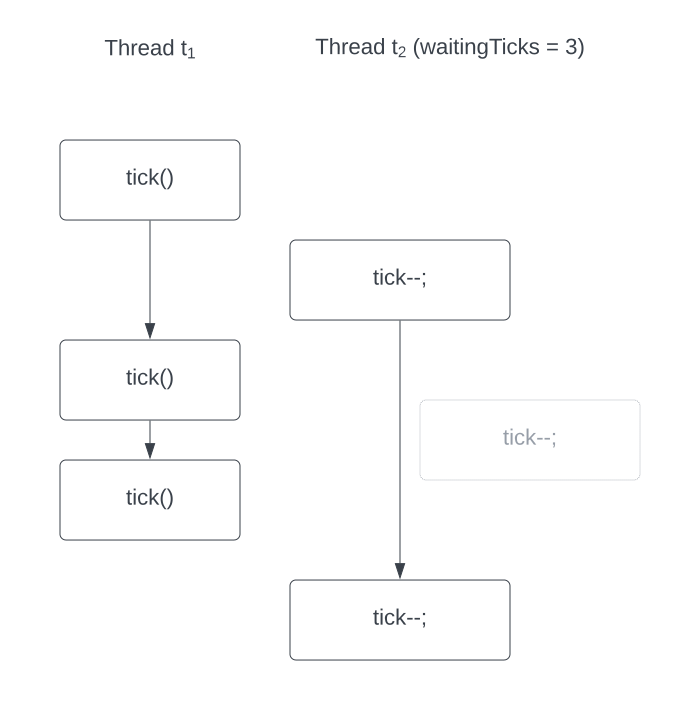
\includegraphics[scale=0.5]{chapters/Anhang/Klausuren/img/tick}
    \caption{Thread $t_1$ ruft 3 mal \texit{tick()} auf. Den Anforderungen nach müsste Thread $t_2$ danach aus der while-wait-Schleife herauskommen, erhält aber nicht die Sperre auf das Objekt von LogicalTime, um seinen eigenen Zähler rechtzeitig zu erniedrigen, bevor $t_1$ erneut \textit{tick()} aufruft. (Quelle: eigene)}
    \label{fig:tick}
\end{figure}

\section{Aufgabe 6}
Auch hier gilt, dass die Aufgabenstellung aufmerksam zu lesen ist.\\
Der Kreis soll erst ausgefüllt werden, wenn die Maustaste gelöst wird.

\begin{minted}[mathescape,
    linenos,
    numbersep=5pt,
    gobble=2,
    frame=lines,
    framesep=2mm]{java}
    private void mousePressed(double x, double y) {
        c = new Circle();
        c.setCenterX(x);
        c.setCenterY(y);
        c.setStroke(Color.RED);
        c.setFill(null); // oder Color.TRANSPARENT
        c.setRadius(RADIUS);
        graphicsPane.getChildren().add(c);
    }

    private void mouseReleased() {
        c.setFill(Color.RED);
        c = null;
    }
\end{minted}

\section{Aufgabe 8}

In der Abbildung \ref{fig:batchmodus} ist links der sequentielle Modus dargestellt, bei dem nach dem Senden einer Nachricht auf die Antwort des Servers gewartet wird, bevor eine neue Nachricht geschickt wird.
Dies wird i.d.R. verwendet, wenn das Senden einer neuen Nachricht abhängig ist von einem Ergebnis, die über die Server-Antwort übermittelt wird, oder wenn mit dem Server interagiert wird (Request abhängig vom Response).\\
Der Batch-Modus auf der rechten Seite der gleichen Abbildung ist schneller, da zwischen dem Senden von Nachrichten nicht auf Antworten gewartet werden müssen. \\
Erst nach dem Senden eine Batches von Nachrichten werden die dem Client zur Verfügung stehenden Antworten ausgelesen.\\

\noindent
In dieser Form des Batch-Modus besteht allerdings die Gefahr, dass es zu Verklemmungen kommt:
\begin{itemize}
    \item Bei dem Client kommen viele Nachrichten an, während er noch sendet.
    \item Die ankommenden Nachrichten für den Client werden gepuffert, bis sie ausgelesen werden (TCP- / OS-seitig).
    \item Läuft der Puffer voll, sorgt die Flusskontrolle (TCP) dafür, dass dem Sender mitgeteilt wird, dass keine Nachrichten mehr empfangen werden können, der Server sendet nicht mehr.
    \item Die zu sendenden Nachrichten des Servers werden in einen Puffer geschrieben.
    \item Der Sende-Puffer des Senders läuft voll.
    \item Bei dem nächsten Sende-Aufruf blockiert der Server, empfangene Nachrichten landen im Empfangspuffer
    \item Der Empfangspuffer des Servers läuft voll, der Client buffert die zu sendenden Nachrichten.
    \item Beide Anwendungen blockieren.
\end{itemize}

\\noindent
Um dieses Problem beim Batch-Modus zu umgehen, werden für das Senden und Empfangen zwei Threads auf Client-Seite erstellt: Ein Thread sendet, ein Thread empfängt. \\
Dadurch kann von dem Client immer wieder sein Empfangspuffer geleert werden, der Server wird beim Senden nicht blockiert.

\begin{figure}
    \centering
    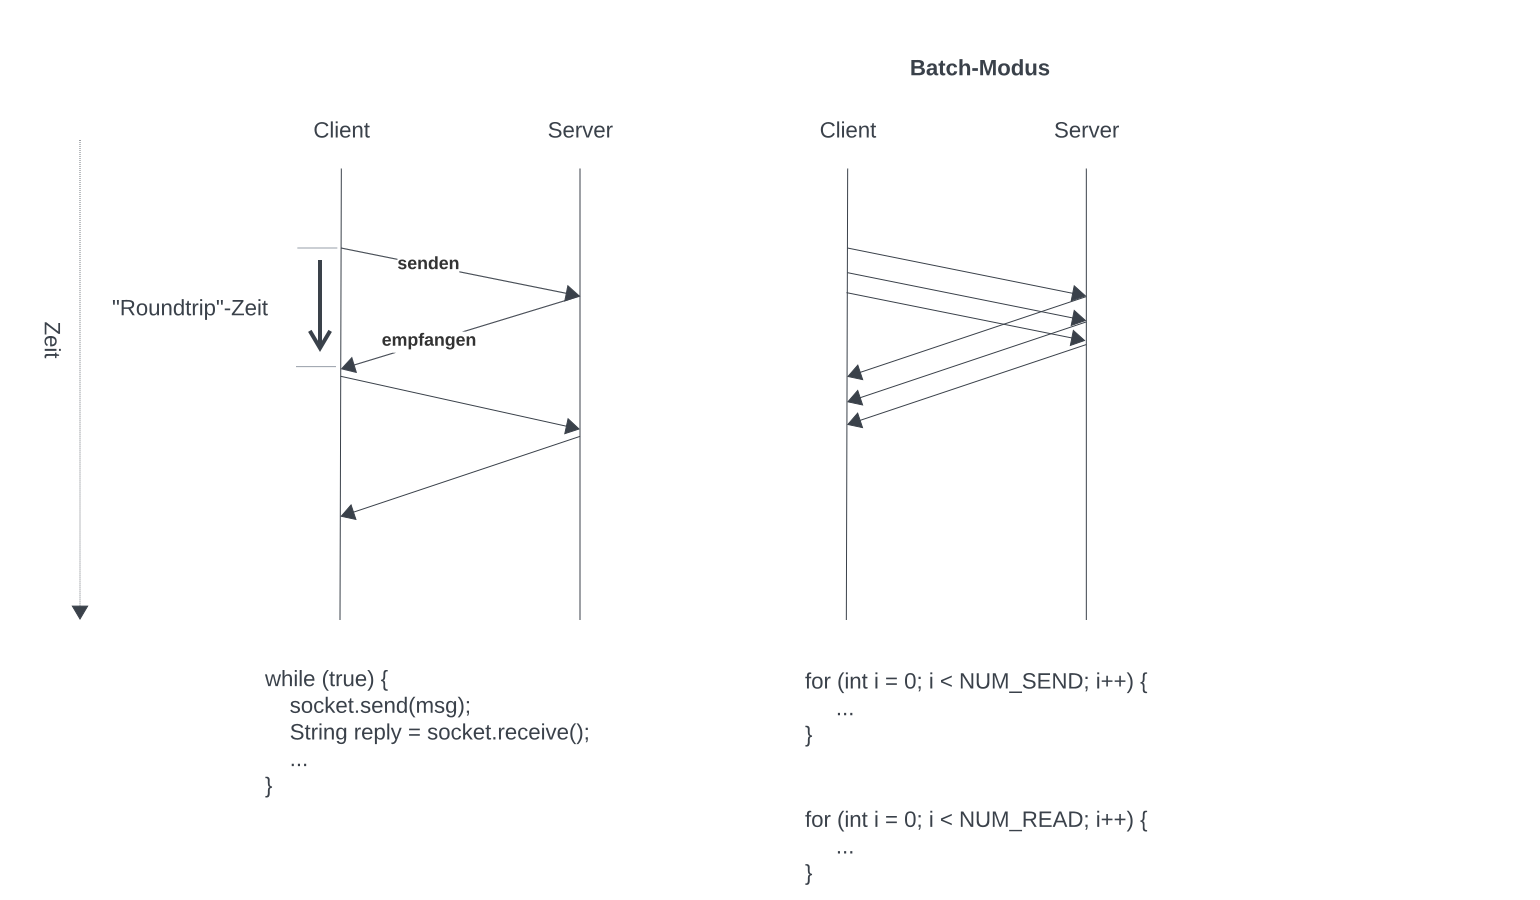
\includegraphics[scale=0.4]{chapters/Anhang/Klausuren/img/batchmodus}
    \caption{Vereinfachte Darstellung sequentieller Kommunikation und Batch-Modus (Quelle: eigene)}
    \label{fig:batchmodus}
\end{figure}
    
\begin{appendices}
    \input{chapters/Anhang/Zusatzaufgaben/index}
    \input{chapters/Anhang/Klausuren/ws13}
    \input{chapters/Anhang/Klausuren/ws15-16}
    \input{chapters/Anhang/Klausuren/ws16-17}
    \input{chapters/Anhang/Klausuren/ss19}
    \input{chapters/Anhang/Präsenzphase/index}

\end{appendices}


\end{appendices}


\end{appendices}



\begin{appendices}
    
\begin{appendices}
    
\begin{appendices}
    \input{chapters/Anhang/Zusatzaufgaben/index}
    \input{chapters/Anhang/Klausuren/ws13}
    \input{chapters/Anhang/Klausuren/ws15-16}
    \input{chapters/Anhang/Klausuren/ws16-17}
    \input{chapters/Anhang/Klausuren/ss19}
    \input{chapters/Anhang/Präsenzphase/index}

\end{appendices}

    \chapter{WS13}\label{ch:klausurws13}

\section{Aufgabe 1}
\subsection{Lösungsvorschlag}


\begin{minted}[mathescape,
    linenos,
    numbersep=5pt,
    gobble=2,
    fontsize=\small,
    frame=lines,
    framesep=2mm]{java}
    class Zahlenschloss {

        private int[] kombination;

        private int[] state;

        private boolean opened = false;

        public Zahlenschloss(int[] kombination) {
            this.kombination = kombination;
            this.state = new int[kombination.length];
        }

        public int anzahlRaedchen() {
            return kombination.length;
        }

        public synchronized int lesen(int radnummer) {
            return state[radnummer];
        }

        public synchronized void drehen(int radnummer, int zahl) {

            state[radnummer] = zahl;
            opened = true;
            for (int i = 0; i < anzahlRaedchen(); i++) {
                if (lesen(i) != kombination[i]) {
                    opened = false;
                    break;
                }
            }

            if (opened) {
                this.notify();
            }
        }

        public synchronized void warten() {

            while (!opened) {
                try {
                    this.wait();
                } catch (InterruptedException ignored) {}
            }
        }
    }
\end{minted}\\


\subsection{Anmerkung und Ergänzungen}

\begin{itemize}
    \item Es wird eine Wartebedingung benötigt, und zwar für die Methode \code{warten()}; ankommende Threads werden
    in die Warteschlange des Zahlenschloss-Objektes geschickt, wenn \code{opened} auf false gesetzt ist, ansonsten
    verlassen diese direkt die Methode wieder.\\
    Die Methode \code{drehen} benötigt keine separate Wartebedingung.
    Es reicht aus, sicherzustellen, dass das Zahlenschloss nicht gleichzeitig von anderen Threads benutzt werden kann:
    Die Methode \code{drehen} ist hierfür synchronisiert, damit das Zahlenschloss {insg.} immer nur eine Zustandsänderung
    erfährt - es sind andere Implementierungen möglich, in denen das Zahlenschloss dann von mehreren Threads gleichzeitig
    genutzt werden darf, wenn sich die Zugriffe anhand der ``Ziel``-\code{radnummer} unterscheiden, {bspw.} durch Mutex-Semaphore,
    die pro Radnummer verwendet werden\footnote{
        der gleichzeitige Zugriff auf unterschiedliche Arrays-Indizes ist erlaubt, s. `´17.4.1. Shared Variables``: \url{https://docs.oracle.com/javase/specs/jls/se21/html/jls-17.html#jls-1.4.1} - abgerufen 14.2.2024
    }.
    \item Es gibt nur eine Wartebedingung, von daher sollte \code{notify()} genügen.\\
    Wenn wir allerdings davon ausgehen, dass mehrere Threads über die Methode \code{warten()} in die Warteschlange des Objektes eingereiht worden sind,  sollte \code{notifyAll()} verwendet werden (siehe hierzu auch Abschnitt \ref{subsec:notifyAll}).
    Dennoch ist nicht garantiert, dass auch alle Threads aus der Warteschlange gelangen, denn es kann sein, dass ein anderer Thread die Methode \code{drehen()} betritt, dort die
    Zahlenkombination ändert und \code{opened} wieder auf \code{false} gesetzt wird. \\
    Ein anderer Thread, der nun in  \code{warten()} an die Reihe kommt, überprüft die Wartebedingung, und wird wieder in die Warteschlange eingereiht.
    Es ist also durchaus möglich, dass ein Thread nicht mehr aus der Methode \code{warten()} herauskommt.\\
    Dies könnte bspw. dadurch verhindert werden, dass die Threads in eine Queue gepackt werden, und in \code{drehen()} eine Wartebedingung eingefügt wird, die erst erfüllt ist,
    wenn die Queue geleert wurde oder aus ihr entnommen wurde, in der Reihenfolge, in der die Threads in die Queue eingereiht worden sind (\textit{FIFO}) (s. a. Abschnitt~\ref{subsec:readerwriterproblem}).
    \item Bei der Teilaufgabe mit der Schleife muss die komplette Schleife synchronisiert werden, was man durch ein \code{synchronized}-Statement erreicht\footnote{siehe Abschnitt~\ref{subsec:synchronizedstatement}.}
    \begin{minted}[mathescape,
        linenos,
        numbersep=5pt,
        gobble=2,
        fontsize=\small,
        frame=lines,
        framesep=2mm]{java}
        synchronized (zk) {
            for (int i = 0; i < anzahlRaedchen; i++) {
                System.out.println(zk.lesen(i));
            }
        }
    \end{minted}
    Ansonsten läuft man Gefahr, dass sich nach Auslesen der 1. Position der Wert von Position 2 geändert hat und dadurch eine
    Zahlenkombination ausgegeben wird, die es nicht gegeben hat:
    \begin{enumerate}
        \item $K\coloneqq[0, 0, 0]$
        \item Position $K_0$ wird ausgelesen und liefert $0$.
        \item Thread ändert $K_0$ zu $1$ $\implies K\coloneqq[1, 0, 0] $.
        \item Thread ändert $K_1$ zu $2$ $\implies K\coloneqq[1, 2, 0] $.
        \item Thread ändert $K_2$ zu $3$ $\implies K\coloneqq[1, 2, 3] $.
        \item Positionen $K_1$ und $K_2$ werden ausgelesen und liefern: $2, 3$
        \item Ausgabe: $0, 2, 3$ - diese Kombination hat es in dem Fall aber tatsächlich nicht gegeben.
    \end{enumerate}
\end{itemize}

\begin{tcolorbox}[colback=red!20,color=white,title=Anmerkung]
    Die Methode \code{lesen()} als \code{synchronized} zu markieren könnte man sich vlt. sparen, wenn man davon ausgeht,
    dass die Methode ohnehin in einem \code{synchronized}-Statement verwendet wird, um alle Rädchen abzulesen.\\
    Mehrere Threads können also nicht parallel auf unterschiedliche Positionen des Feldes zugreifen, wenn die Methode
    synchronisiert ist.\\
    Allerdings ist sowohl das Skript als auch das Buch recht klar, was in dieser Situation geschehen muss (s. Skript Fopt1/2, S. 9, außerdem \cite[31, Abschnitt 2.3.6]{Oec22}): Es muss (in diesem Kurs) immer \code{synchronized} verwendet werden, wenn gleichzeitig
    Daten geschrieben und gleichzeitig diese Daten gelesen werden sollen - und eine andere Implementierung, bei der die
    einzelnen Positionen ``gelocked`` sind, so dass ein gleichzeitiger Zugriff auf unterschiedliche Rädchen möglich ist, war nicht gefordert.\\
    Ggfl. würde in anderen Implementierungen der Einsatz von \code{AtomicReferenceArray}\footnote{s. \cite[157 ff.]{Oec22}
    s. ``Class AtomicReferenceArray<E>``: \url{https://docs.oracle.com/en/java/javase/21/docs/api/java.base/java/util/concurrent/atomic/AtomicReferenceArray.html} - abgerufen 15.2.2024
    } Sinn machen, aber das Lehrmaterial ist bereits sehr eindeutig bzgl. der Verwendung von \code{synchronized}.
\end{tcolorbox}



\section{Aufgabe 3}
\subsection{Lösungsvorschlag}

\subsection*{Statische Parallelität}
Statische Parallelität erlaubt es einem Server, eine \textit{fixe} Anzahl von Verbindungen gleichzeitig zu bedienen.\\
Hierbei wird ein Feld von Threads erstellt, wobei jeder Thread das \code{ServerSocket}-Objekt als Referenz übergeben bekommt.
In der \code{run()}-Methode wird dann über \code{accept()} in einer Endlosschleife auf eingehende Verbindungen gewartet, die dann so lange bedient werden, bis sich ein Client wieder abmeldet (oder eine andere Abbruchbedingung erfüllt ist, wie z.B. ein \code{SocketTimeout}).\\
Das sich ein Client abmeldet, bekommt man bspw. dadurch mit, dass \code{null} beim Lesen von einer Nachricht des Clients zurückgegeben wird (vgl. \cite[286]{Oec22}. \\
Siehe Abschnitt~\ref{sec:seqparserver} für ein Implementierungsbeispiel.



\subsection*{Dynamische Parallelität}

Bei der \textbf{Dynamischer Parallelität} erzeugt der Server für jede Verbindung einen neuen Thread, der so lange läuft, bis der Client die Verbindung wieder trennt.\\
Die Anzahl der Threads ändert sich dadurch laufend.\\
Wird die max. Anzahl erlaubter Threads nicht kontrolliert, kann es zu einer Überlastung des Server-Rechners kommen (bspw. durch einen Denial-of-Service-Angriff.)\\

\noindent
I.d.R. ist eine Mischform aus beidem geeignet, um mehrere Clients gleichzeitig bedienen zu können, und dabei nicht Gefahr zu laufen, durch dynamisches, unbegrenztes Wachstum der Anzahl der Threads überlastet zu werden.

    \chapter{WS13}\label{ch:klausurws5-16}

\section{Rechteck-Scroll (SS15 Aufgabe 2)}

Aufgabenstellung unklar.\\
Mögliche Implementierung unter \url{https://github.com/ThorstenSuckow/fopt/tree/main/src/main/java/klausurvorbereitung/foptws1516/MouseDragsSquareDemo}.

\section{Rechteck-Scroll (WS15/16 Aufgabe 1)}

Aufgabenstellung unklar.\\
Mögliche Implementierung unter \url{https://github.com/ThorstenSuckow/fopt/tree/main/src/main/java/klausurvorbereitung/foptws1516/MaxWeightDemo}.\\

\noindent
Es gibt nur eine Warteschlange für Threads in \code{use()}, es gibt keine Wartebedingung in \code{dontUse()} und damit auch keine weitere Warteschlange.\\
Es sind durch die Zugriffe auf unterschiedliche Indizes allerdings mehrere Wartebedingungen vorhanden, weshalb hab \code{notifyAll()} nutzen sollte,
sobald ein Zugriff auf ein Feld nach Aufruf von \code{dontUse} wieder möglich wird.\\
Ansonsten bestünde die Gefahr, dass bei dem Einsatz von \code{notify()} ein wartender Thread nicht geweckt wird, obwohl er weiterlaufen könnte:\\
Angenommen, das Feld $F$ hat eine Länge von $3$, das \code{maxWeight} ist mit $2$ konfiguriert.
Thread $t_1$ mit einer Laufzeit von $200\ sek$ bekommt Zugriff auf $F_0$, setzt $currentWeight$ auf $1$.\\
Thread $t_2$ mit einer Laufzeit von $1\ sek$ möchte auf $F_1$ zugreifen, setzt $currentWeight=2$ in die Warteschlange.\\
Thread $t_3$ meldet Zugriff auf $F_0$ an und gelangt in die Warteschlange.\\
Thread $t_4$ meldet Zugriff auf $F_1$ an und gelangt in die Warteschlange.\\
Thread $t_2$ ist mit der Bearbeitung von $F_1$ fertig, $currentWeight$ wird auf $1$ gesetzt, \code{notify()} wird aufgerufen.\\
Thread $t_3$ wird aus der Warteschlange geholt, kann aber nicht weiterarbeiten, da $F_0$ noch durch den länger dauernden $t_1$ blockiert ist, und kommt wieder in die Warteschlange.\\

\noindent
Offensichtlich hätte in dem Beispiel \code{notifyAll()} dazu geführt, dass auch $T_4$ seine Wartebedingung hätte überprüfen können, und hätte so Zugriff auf $F_1$ bekommen.
Stattdessen muss nun gewartet werden, bis das nächste \code{notify()} aufgerufen wird, oder ein neu ankommender Thread $F_1$ belegt.

    \chapter{WS16-17}\label{ch:klausurws16-17}

\section{Aufgabe 1}
\subsection{Lösungshinweis}

Die erste Aufgabe verdeutlicht, was bei einem \code{notifyAll()} und unsauber gesetzten Wartebedingungen passieren kann.\\
Sei folgender Quellcode gegeben:


\begin{minted}[mathescape,
    linenos,
    numbersep=5pt,
    gobble=2,
    fontsize=\small,
    frame=lines,
    framesep=2mm]{java}
    class Cond1AndCond2 {

        private boolean cond1;
        private boolean cond2;

        public synchronized void setCond1(boolean c) {
            cond1 = c;
            notifyAll();
        }

        public synchronized void setCond2(boolean c) {
            cond2 = c;
            notifyAll();
        }

        public synchronized void cond1AndCond2() {
            while(!cond1) {
                try {
                    wait();
                } catch(InterruptedException e) { }
            }

            while(!cond2) {
                try {
                    wait();
                } catch(InterruptedException e) {}
            }
            System.out.println("cond1 and cond2:" + cond1 + " " + cond2);
        }
    }
\end{minted}\\

Man sollte auf den ersten Blick meinen, dass \code{cond1} und \code{cond2} beide \code{true} sein müssen, damit die Ausgabe erfolgt.\\
Tatsächlich ist es aber so, dass es in der Methode zwei unterschiedliche Wartebedingungen gibt.\\
Die erste Wartebedingung schickt einen Thread in die Warteschlange, wenn \code{cond1 == false} gilt.\\
Setzt ein anderer Thread über \code{setCond1(true)} das Attribut entsprechend auf \code{true}, bewirkt der nachfolgende Aufruf von \code{notifyAll()}, dass alle \textit{wartenden} Threads aus der Warteschlange entfernt werden und erneut um eine Sperre des Objektes konkurrieren.\\
Erhält ein entsprechender Thread $t_w$ die Sperre auf das Objekt und kann seine \textit{while-wait-Schleife} verlassen, kann es vorkommen, dass er erneut in die Warteschlange eingereiht wird, wegen der nachfolgenden Wartebedingung \code{cond2 == false}.\\
Angenommen, ein weiterer Thread ruft nun \code{setCond2(true)} auf, und $t_w$ kommt aus der Warteschlange und konkurriert erneut und um die Sperre des Objektes, dann kann es vorkommen, das ein anderer Thread zunächst die Sperre erhält, \code{cond1} wieder auf \code{false} setzt, dann erhält $t_w$ die Sperre, überprüft die Wartebedingung \code{cond2 == false}.\\
Wegen \code{cond2} gelangt er aus der \textit{while-wait-Schleife} und die Ausgabe erfolgt - da zwischenzeitlich \code{cond1} wieder auf \code{false} gesetzt wurde, ist die erwartete Ausgabe nicht \code{true true}, sondern \code{false true} (s. Abbildung \ref{fig:cond1cond2}).\\

\begin{figure}
    \centering
    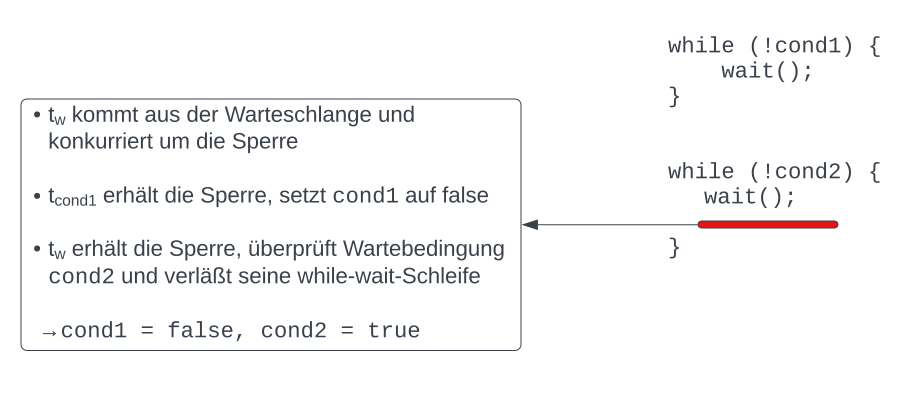
\includegraphics[scale=0.4]{chapters/Anhang/Klausuren/img/cond1cond2}
    \caption{in den rot markierten Bereich konkurriert $t_w$ um die Sperre des Objektes - wenn durch einen anderen Thread, der vor $t_w$ die Sperre erhält, \textit{cond1} auf \textit{false} gesetzt wird, stimmt die Ausgabe nicht mit der erwarteten überein. (Quelle: eigene)}
    \label{fig:cond1cond2}
\end{figure}

\noindent
Die korrekte Wartebedingung sollte lauten:

\begin{minted}[mathescape,
    linenos,
    numbersep=5pt,
    gobble=2,
    fontsize=\small,
    frame=lines,
    framesep=2mm]{java}
    public synchronized void cond1AndCond2() {
        while(!cond1 || !cond2) {
            try {
                wait();
            } catch(InterruptedException e) { }
        }
        System.out.println("cond1 and cond2:" + cond1 + " " + cond2);
    }
\end{minted}\\

Darüber hinaus müßte \code{notifyAll()} nur aufgerufen werden, wenn sowohl \code{cond1} als auch \code{cond2} auf \code{true} gesetzt sind, was leicht in den entsprechenden Methoden überprüft werden kann.
    \chapter{SS19}\label{ch:klausurss19}

\section{Aufgabe 1}

Bei der Aufgabe ist es wichtig, die Anforderungen genau zu beachten.\\
Ob eine Thread die while-wait-Schleife verlassen darf, wird von der Methode \code{tick()} gesteuert - wieviele Ticks ein Thread in der Schleife bleiben soll, wird von dem jeweiligen Thread definiert.\\
Die \code{tick()}-Methode wird von anderen Threads aufgerufen, es kann also durchaus vorkommen, dass mehrmals hintereinander
die \code{notifyAll()}-Methode aufgerufen wird - diese entfernt alle Threads aus der Warteschlange, damit die Threads ihre
Wartebedingungen erneut überprüfen können.\\
da \code{tick()} aber auch gleichzeitig einen Zähler realisieren soll, \textit{muss} es in der Methode auch eine Zählvariable geben, anhand derer die in der while-wait-Schleife enthaltenen Threads feststellen können, wie oft \code{tick()} aufgerufen wurde, um entsprechend aus der Schleife und nachfolgend der Methode herauszukommen.

\begin{figure}
    \centering
    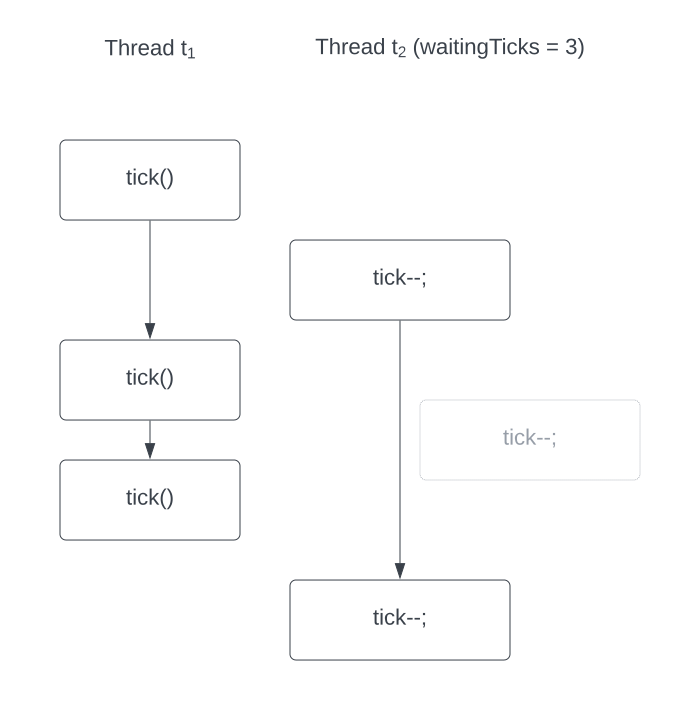
\includegraphics[scale=0.5]{chapters/Anhang/Klausuren/img/tick}
    \caption{Thread $t_1$ ruft 3 mal \texit{tick()} auf. Den Anforderungen nach müsste Thread $t_2$ danach aus der while-wait-Schleife herauskommen, erhält aber nicht die Sperre auf das Objekt von LogicalTime, um seinen eigenen Zähler rechtzeitig zu erniedrigen, bevor $t_1$ erneut \textit{tick()} aufruft. (Quelle: eigene)}
    \label{fig:tick}
\end{figure}

\section{Aufgabe 6}
Auch hier gilt, dass die Aufgabenstellung aufmerksam zu lesen ist.\\
Der Kreis soll erst ausgefüllt werden, wenn die Maustaste gelöst wird.

\begin{minted}[mathescape,
    linenos,
    numbersep=5pt,
    gobble=2,
    frame=lines,
    framesep=2mm]{java}
    private void mousePressed(double x, double y) {
        c = new Circle();
        c.setCenterX(x);
        c.setCenterY(y);
        c.setStroke(Color.RED);
        c.setFill(null); // oder Color.TRANSPARENT
        c.setRadius(RADIUS);
        graphicsPane.getChildren().add(c);
    }

    private void mouseReleased() {
        c.setFill(Color.RED);
        c = null;
    }
\end{minted}

\section{Aufgabe 8}

In der Abbildung \ref{fig:batchmodus} ist links der sequentielle Modus dargestellt, bei dem nach dem Senden einer Nachricht auf die Antwort des Servers gewartet wird, bevor eine neue Nachricht geschickt wird.
Dies wird i.d.R. verwendet, wenn das Senden einer neuen Nachricht abhängig ist von einem Ergebnis, die über die Server-Antwort übermittelt wird, oder wenn mit dem Server interagiert wird (Request abhängig vom Response).\\
Der Batch-Modus auf der rechten Seite der gleichen Abbildung ist schneller, da zwischen dem Senden von Nachrichten nicht auf Antworten gewartet werden müssen. \\
Erst nach dem Senden eine Batches von Nachrichten werden die dem Client zur Verfügung stehenden Antworten ausgelesen.\\

\noindent
In dieser Form des Batch-Modus besteht allerdings die Gefahr, dass es zu Verklemmungen kommt:
\begin{itemize}
    \item Bei dem Client kommen viele Nachrichten an, während er noch sendet.
    \item Die ankommenden Nachrichten für den Client werden gepuffert, bis sie ausgelesen werden (TCP- / OS-seitig).
    \item Läuft der Puffer voll, sorgt die Flusskontrolle (TCP) dafür, dass dem Sender mitgeteilt wird, dass keine Nachrichten mehr empfangen werden können, der Server sendet nicht mehr.
    \item Die zu sendenden Nachrichten des Servers werden in einen Puffer geschrieben.
    \item Der Sende-Puffer des Senders läuft voll.
    \item Bei dem nächsten Sende-Aufruf blockiert der Server, empfangene Nachrichten landen im Empfangspuffer
    \item Der Empfangspuffer des Servers läuft voll, der Client buffert die zu sendenden Nachrichten.
    \item Beide Anwendungen blockieren.
\end{itemize}

\\noindent
Um dieses Problem beim Batch-Modus zu umgehen, werden für das Senden und Empfangen zwei Threads auf Client-Seite erstellt: Ein Thread sendet, ein Thread empfängt. \\
Dadurch kann von dem Client immer wieder sein Empfangspuffer geleert werden, der Server wird beim Senden nicht blockiert.

\begin{figure}
    \centering
    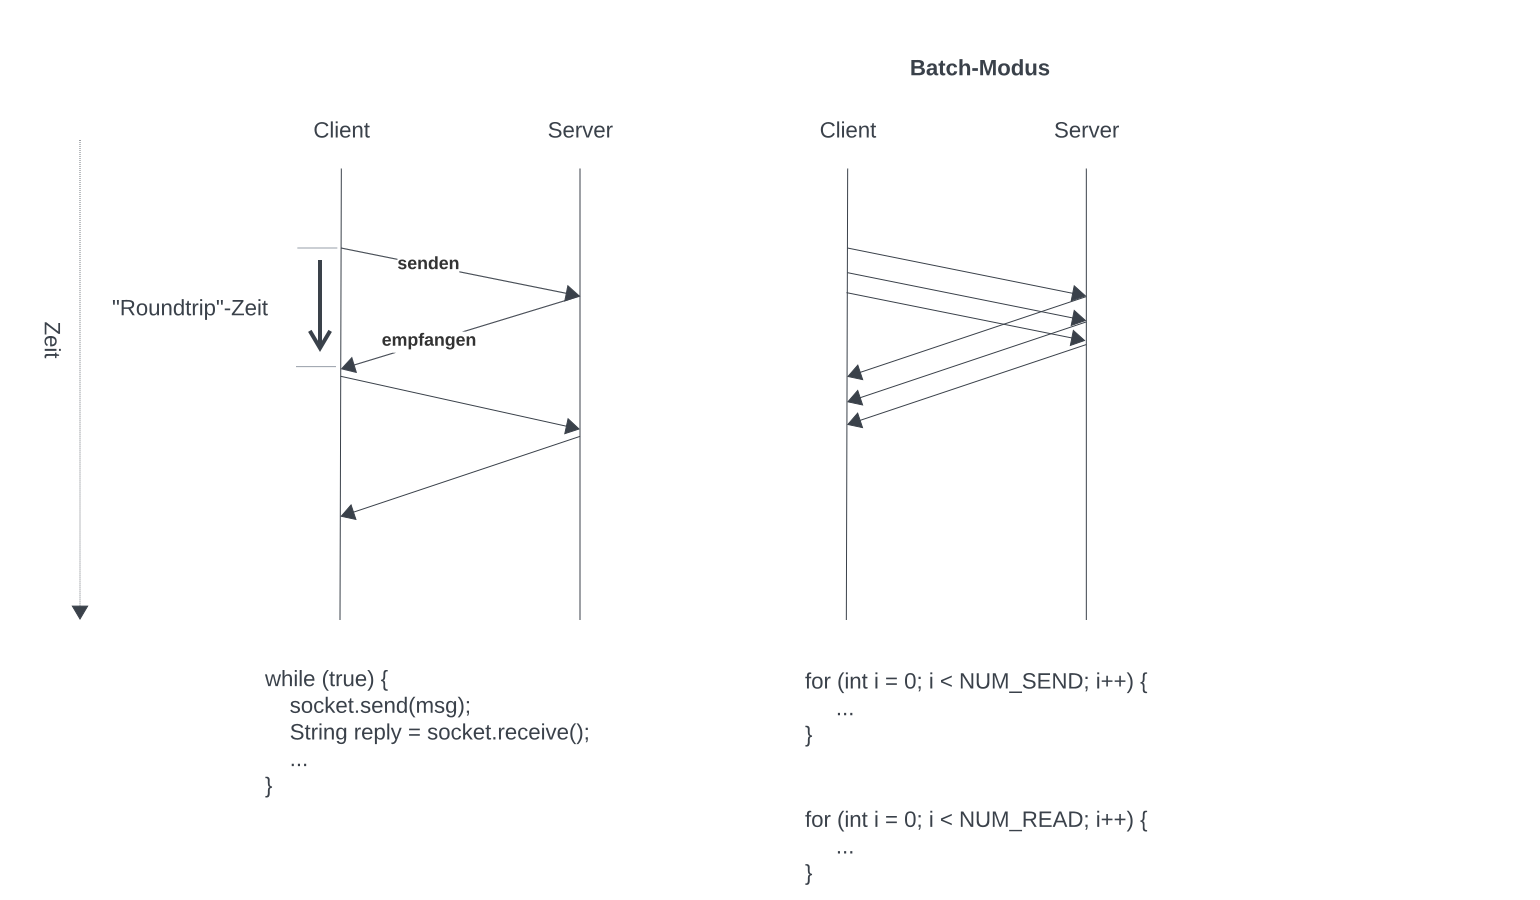
\includegraphics[scale=0.4]{chapters/Anhang/Klausuren/img/batchmodus}
    \caption{Vereinfachte Darstellung sequentieller Kommunikation und Batch-Modus (Quelle: eigene)}
    \label{fig:batchmodus}
\end{figure}
    
\begin{appendices}
    \input{chapters/Anhang/Zusatzaufgaben/index}
    \input{chapters/Anhang/Klausuren/ws13}
    \input{chapters/Anhang/Klausuren/ws15-16}
    \input{chapters/Anhang/Klausuren/ws16-17}
    \input{chapters/Anhang/Klausuren/ss19}
    \input{chapters/Anhang/Präsenzphase/index}

\end{appendices}


\end{appendices}

    \chapter{WS13}\label{ch:klausurws13}

\section{Aufgabe 1}
\subsection{Lösungsvorschlag}


\begin{minted}[mathescape,
    linenos,
    numbersep=5pt,
    gobble=2,
    fontsize=\small,
    frame=lines,
    framesep=2mm]{java}
    class Zahlenschloss {

        private int[] kombination;

        private int[] state;

        private boolean opened = false;

        public Zahlenschloss(int[] kombination) {
            this.kombination = kombination;
            this.state = new int[kombination.length];
        }

        public int anzahlRaedchen() {
            return kombination.length;
        }

        public synchronized int lesen(int radnummer) {
            return state[radnummer];
        }

        public synchronized void drehen(int radnummer, int zahl) {

            state[radnummer] = zahl;
            opened = true;
            for (int i = 0; i < anzahlRaedchen(); i++) {
                if (lesen(i) != kombination[i]) {
                    opened = false;
                    break;
                }
            }

            if (opened) {
                this.notify();
            }
        }

        public synchronized void warten() {

            while (!opened) {
                try {
                    this.wait();
                } catch (InterruptedException ignored) {}
            }
        }
    }
\end{minted}\\


\subsection{Anmerkung und Ergänzungen}

\begin{itemize}
    \item Es wird eine Wartebedingung benötigt, und zwar für die Methode \code{warten()}; ankommende Threads werden
    in die Warteschlange des Zahlenschloss-Objektes geschickt, wenn \code{opened} auf false gesetzt ist, ansonsten
    verlassen diese direkt die Methode wieder.\\
    Die Methode \code{drehen} benötigt keine separate Wartebedingung.
    Es reicht aus, sicherzustellen, dass das Zahlenschloss nicht gleichzeitig von anderen Threads benutzt werden kann:
    Die Methode \code{drehen} ist hierfür synchronisiert, damit das Zahlenschloss {insg.} immer nur eine Zustandsänderung
    erfährt - es sind andere Implementierungen möglich, in denen das Zahlenschloss dann von mehreren Threads gleichzeitig
    genutzt werden darf, wenn sich die Zugriffe anhand der ``Ziel``-\code{radnummer} unterscheiden, {bspw.} durch Mutex-Semaphore,
    die pro Radnummer verwendet werden\footnote{
        der gleichzeitige Zugriff auf unterschiedliche Arrays-Indizes ist erlaubt, s. `´17.4.1. Shared Variables``: \url{https://docs.oracle.com/javase/specs/jls/se21/html/jls-17.html#jls-1.4.1} - abgerufen 14.2.2024
    }.
    \item Es gibt nur eine Wartebedingung, von daher sollte \code{notify()} genügen.\\
    Wenn wir allerdings davon ausgehen, dass mehrere Threads über die Methode \code{warten()} in die Warteschlange des Objektes eingereiht worden sind,  sollte \code{notifyAll()} verwendet werden (siehe hierzu auch Abschnitt \ref{subsec:notifyAll}).
    Dennoch ist nicht garantiert, dass auch alle Threads aus der Warteschlange gelangen, denn es kann sein, dass ein anderer Thread die Methode \code{drehen()} betritt, dort die
    Zahlenkombination ändert und \code{opened} wieder auf \code{false} gesetzt wird. \\
    Ein anderer Thread, der nun in  \code{warten()} an die Reihe kommt, überprüft die Wartebedingung, und wird wieder in die Warteschlange eingereiht.
    Es ist also durchaus möglich, dass ein Thread nicht mehr aus der Methode \code{warten()} herauskommt.\\
    Dies könnte bspw. dadurch verhindert werden, dass die Threads in eine Queue gepackt werden, und in \code{drehen()} eine Wartebedingung eingefügt wird, die erst erfüllt ist,
    wenn die Queue geleert wurde oder aus ihr entnommen wurde, in der Reihenfolge, in der die Threads in die Queue eingereiht worden sind (\textit{FIFO}) (s. a. Abschnitt~\ref{subsec:readerwriterproblem}).
    \item Bei der Teilaufgabe mit der Schleife muss die komplette Schleife synchronisiert werden, was man durch ein \code{synchronized}-Statement erreicht\footnote{siehe Abschnitt~\ref{subsec:synchronizedstatement}.}
    \begin{minted}[mathescape,
        linenos,
        numbersep=5pt,
        gobble=2,
        fontsize=\small,
        frame=lines,
        framesep=2mm]{java}
        synchronized (zk) {
            for (int i = 0; i < anzahlRaedchen; i++) {
                System.out.println(zk.lesen(i));
            }
        }
    \end{minted}
    Ansonsten läuft man Gefahr, dass sich nach Auslesen der 1. Position der Wert von Position 2 geändert hat und dadurch eine
    Zahlenkombination ausgegeben wird, die es nicht gegeben hat:
    \begin{enumerate}
        \item $K\coloneqq[0, 0, 0]$
        \item Position $K_0$ wird ausgelesen und liefert $0$.
        \item Thread ändert $K_0$ zu $1$ $\implies K\coloneqq[1, 0, 0] $.
        \item Thread ändert $K_1$ zu $2$ $\implies K\coloneqq[1, 2, 0] $.
        \item Thread ändert $K_2$ zu $3$ $\implies K\coloneqq[1, 2, 3] $.
        \item Positionen $K_1$ und $K_2$ werden ausgelesen und liefern: $2, 3$
        \item Ausgabe: $0, 2, 3$ - diese Kombination hat es in dem Fall aber tatsächlich nicht gegeben.
    \end{enumerate}
\end{itemize}

\begin{tcolorbox}[colback=red!20,color=white,title=Anmerkung]
    Die Methode \code{lesen()} als \code{synchronized} zu markieren könnte man sich vlt. sparen, wenn man davon ausgeht,
    dass die Methode ohnehin in einem \code{synchronized}-Statement verwendet wird, um alle Rädchen abzulesen.\\
    Mehrere Threads können also nicht parallel auf unterschiedliche Positionen des Feldes zugreifen, wenn die Methode
    synchronisiert ist.\\
    Allerdings ist sowohl das Skript als auch das Buch recht klar, was in dieser Situation geschehen muss (s. Skript Fopt1/2, S. 9, außerdem \cite[31, Abschnitt 2.3.6]{Oec22}): Es muss (in diesem Kurs) immer \code{synchronized} verwendet werden, wenn gleichzeitig
    Daten geschrieben und gleichzeitig diese Daten gelesen werden sollen - und eine andere Implementierung, bei der die
    einzelnen Positionen ``gelocked`` sind, so dass ein gleichzeitiger Zugriff auf unterschiedliche Rädchen möglich ist, war nicht gefordert.\\
    Ggfl. würde in anderen Implementierungen der Einsatz von \code{AtomicReferenceArray}\footnote{s. \cite[157 ff.]{Oec22}
    s. ``Class AtomicReferenceArray<E>``: \url{https://docs.oracle.com/en/java/javase/21/docs/api/java.base/java/util/concurrent/atomic/AtomicReferenceArray.html} - abgerufen 15.2.2024
    } Sinn machen, aber das Lehrmaterial ist bereits sehr eindeutig bzgl. der Verwendung von \code{synchronized}.
\end{tcolorbox}



\section{Aufgabe 3}
\subsection{Lösungsvorschlag}

\subsection*{Statische Parallelität}
Statische Parallelität erlaubt es einem Server, eine \textit{fixe} Anzahl von Verbindungen gleichzeitig zu bedienen.\\
Hierbei wird ein Feld von Threads erstellt, wobei jeder Thread das \code{ServerSocket}-Objekt als Referenz übergeben bekommt.
In der \code{run()}-Methode wird dann über \code{accept()} in einer Endlosschleife auf eingehende Verbindungen gewartet, die dann so lange bedient werden, bis sich ein Client wieder abmeldet (oder eine andere Abbruchbedingung erfüllt ist, wie z.B. ein \code{SocketTimeout}).\\
Das sich ein Client abmeldet, bekommt man bspw. dadurch mit, dass \code{null} beim Lesen von einer Nachricht des Clients zurückgegeben wird (vgl. \cite[286]{Oec22}. \\
Siehe Abschnitt~\ref{sec:seqparserver} für ein Implementierungsbeispiel.



\subsection*{Dynamische Parallelität}

Bei der \textbf{Dynamischer Parallelität} erzeugt der Server für jede Verbindung einen neuen Thread, der so lange läuft, bis der Client die Verbindung wieder trennt.\\
Die Anzahl der Threads ändert sich dadurch laufend.\\
Wird die max. Anzahl erlaubter Threads nicht kontrolliert, kann es zu einer Überlastung des Server-Rechners kommen (bspw. durch einen Denial-of-Service-Angriff.)\\

\noindent
I.d.R. ist eine Mischform aus beidem geeignet, um mehrere Clients gleichzeitig bedienen zu können, und dabei nicht Gefahr zu laufen, durch dynamisches, unbegrenztes Wachstum der Anzahl der Threads überlastet zu werden.

    \chapter{WS13}\label{ch:klausurws5-16}

\section{Rechteck-Scroll (SS15 Aufgabe 2)}

Aufgabenstellung unklar.\\
Mögliche Implementierung unter \url{https://github.com/ThorstenSuckow/fopt/tree/main/src/main/java/klausurvorbereitung/foptws1516/MouseDragsSquareDemo}.

\section{Rechteck-Scroll (WS15/16 Aufgabe 1)}

Aufgabenstellung unklar.\\
Mögliche Implementierung unter \url{https://github.com/ThorstenSuckow/fopt/tree/main/src/main/java/klausurvorbereitung/foptws1516/MaxWeightDemo}.\\

\noindent
Es gibt nur eine Warteschlange für Threads in \code{use()}, es gibt keine Wartebedingung in \code{dontUse()} und damit auch keine weitere Warteschlange.\\
Es sind durch die Zugriffe auf unterschiedliche Indizes allerdings mehrere Wartebedingungen vorhanden, weshalb hab \code{notifyAll()} nutzen sollte,
sobald ein Zugriff auf ein Feld nach Aufruf von \code{dontUse} wieder möglich wird.\\
Ansonsten bestünde die Gefahr, dass bei dem Einsatz von \code{notify()} ein wartender Thread nicht geweckt wird, obwohl er weiterlaufen könnte:\\
Angenommen, das Feld $F$ hat eine Länge von $3$, das \code{maxWeight} ist mit $2$ konfiguriert.
Thread $t_1$ mit einer Laufzeit von $200\ sek$ bekommt Zugriff auf $F_0$, setzt $currentWeight$ auf $1$.\\
Thread $t_2$ mit einer Laufzeit von $1\ sek$ möchte auf $F_1$ zugreifen, setzt $currentWeight=2$ in die Warteschlange.\\
Thread $t_3$ meldet Zugriff auf $F_0$ an und gelangt in die Warteschlange.\\
Thread $t_4$ meldet Zugriff auf $F_1$ an und gelangt in die Warteschlange.\\
Thread $t_2$ ist mit der Bearbeitung von $F_1$ fertig, $currentWeight$ wird auf $1$ gesetzt, \code{notify()} wird aufgerufen.\\
Thread $t_3$ wird aus der Warteschlange geholt, kann aber nicht weiterarbeiten, da $F_0$ noch durch den länger dauernden $t_1$ blockiert ist, und kommt wieder in die Warteschlange.\\

\noindent
Offensichtlich hätte in dem Beispiel \code{notifyAll()} dazu geführt, dass auch $T_4$ seine Wartebedingung hätte überprüfen können, und hätte so Zugriff auf $F_1$ bekommen.
Stattdessen muss nun gewartet werden, bis das nächste \code{notify()} aufgerufen wird, oder ein neu ankommender Thread $F_1$ belegt.

    \chapter{WS16-17}\label{ch:klausurws16-17}

\section{Aufgabe 1}
\subsection{Lösungshinweis}

Die erste Aufgabe verdeutlicht, was bei einem \code{notifyAll()} und unsauber gesetzten Wartebedingungen passieren kann.\\
Sei folgender Quellcode gegeben:


\begin{minted}[mathescape,
    linenos,
    numbersep=5pt,
    gobble=2,
    fontsize=\small,
    frame=lines,
    framesep=2mm]{java}
    class Cond1AndCond2 {

        private boolean cond1;
        private boolean cond2;

        public synchronized void setCond1(boolean c) {
            cond1 = c;
            notifyAll();
        }

        public synchronized void setCond2(boolean c) {
            cond2 = c;
            notifyAll();
        }

        public synchronized void cond1AndCond2() {
            while(!cond1) {
                try {
                    wait();
                } catch(InterruptedException e) { }
            }

            while(!cond2) {
                try {
                    wait();
                } catch(InterruptedException e) {}
            }
            System.out.println("cond1 and cond2:" + cond1 + " " + cond2);
        }
    }
\end{minted}\\

Man sollte auf den ersten Blick meinen, dass \code{cond1} und \code{cond2} beide \code{true} sein müssen, damit die Ausgabe erfolgt.\\
Tatsächlich ist es aber so, dass es in der Methode zwei unterschiedliche Wartebedingungen gibt.\\
Die erste Wartebedingung schickt einen Thread in die Warteschlange, wenn \code{cond1 == false} gilt.\\
Setzt ein anderer Thread über \code{setCond1(true)} das Attribut entsprechend auf \code{true}, bewirkt der nachfolgende Aufruf von \code{notifyAll()}, dass alle \textit{wartenden} Threads aus der Warteschlange entfernt werden und erneut um eine Sperre des Objektes konkurrieren.\\
Erhält ein entsprechender Thread $t_w$ die Sperre auf das Objekt und kann seine \textit{while-wait-Schleife} verlassen, kann es vorkommen, dass er erneut in die Warteschlange eingereiht wird, wegen der nachfolgenden Wartebedingung \code{cond2 == false}.\\
Angenommen, ein weiterer Thread ruft nun \code{setCond2(true)} auf, und $t_w$ kommt aus der Warteschlange und konkurriert erneut und um die Sperre des Objektes, dann kann es vorkommen, das ein anderer Thread zunächst die Sperre erhält, \code{cond1} wieder auf \code{false} setzt, dann erhält $t_w$ die Sperre, überprüft die Wartebedingung \code{cond2 == false}.\\
Wegen \code{cond2} gelangt er aus der \textit{while-wait-Schleife} und die Ausgabe erfolgt - da zwischenzeitlich \code{cond1} wieder auf \code{false} gesetzt wurde, ist die erwartete Ausgabe nicht \code{true true}, sondern \code{false true} (s. Abbildung \ref{fig:cond1cond2}).\\

\begin{figure}
    \centering
    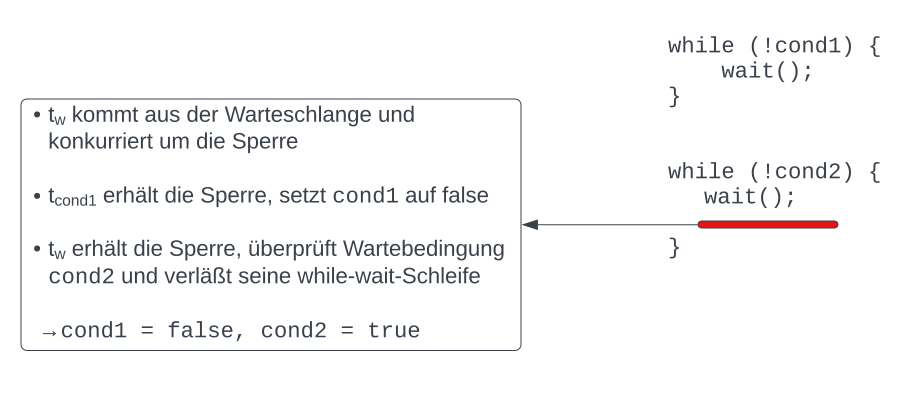
\includegraphics[scale=0.4]{chapters/Anhang/Klausuren/img/cond1cond2}
    \caption{in den rot markierten Bereich konkurriert $t_w$ um die Sperre des Objektes - wenn durch einen anderen Thread, der vor $t_w$ die Sperre erhält, \textit{cond1} auf \textit{false} gesetzt wird, stimmt die Ausgabe nicht mit der erwarteten überein. (Quelle: eigene)}
    \label{fig:cond1cond2}
\end{figure}

\noindent
Die korrekte Wartebedingung sollte lauten:

\begin{minted}[mathescape,
    linenos,
    numbersep=5pt,
    gobble=2,
    fontsize=\small,
    frame=lines,
    framesep=2mm]{java}
    public synchronized void cond1AndCond2() {
        while(!cond1 || !cond2) {
            try {
                wait();
            } catch(InterruptedException e) { }
        }
        System.out.println("cond1 and cond2:" + cond1 + " " + cond2);
    }
\end{minted}\\

Darüber hinaus müßte \code{notifyAll()} nur aufgerufen werden, wenn sowohl \code{cond1} als auch \code{cond2} auf \code{true} gesetzt sind, was leicht in den entsprechenden Methoden überprüft werden kann.
    \chapter{SS19}\label{ch:klausurss19}

\section{Aufgabe 1}

Bei der Aufgabe ist es wichtig, die Anforderungen genau zu beachten.\\
Ob eine Thread die while-wait-Schleife verlassen darf, wird von der Methode \code{tick()} gesteuert - wieviele Ticks ein Thread in der Schleife bleiben soll, wird von dem jeweiligen Thread definiert.\\
Die \code{tick()}-Methode wird von anderen Threads aufgerufen, es kann also durchaus vorkommen, dass mehrmals hintereinander
die \code{notifyAll()}-Methode aufgerufen wird - diese entfernt alle Threads aus der Warteschlange, damit die Threads ihre
Wartebedingungen erneut überprüfen können.\\
da \code{tick()} aber auch gleichzeitig einen Zähler realisieren soll, \textit{muss} es in der Methode auch eine Zählvariable geben, anhand derer die in der while-wait-Schleife enthaltenen Threads feststellen können, wie oft \code{tick()} aufgerufen wurde, um entsprechend aus der Schleife und nachfolgend der Methode herauszukommen.

\begin{figure}
    \centering
    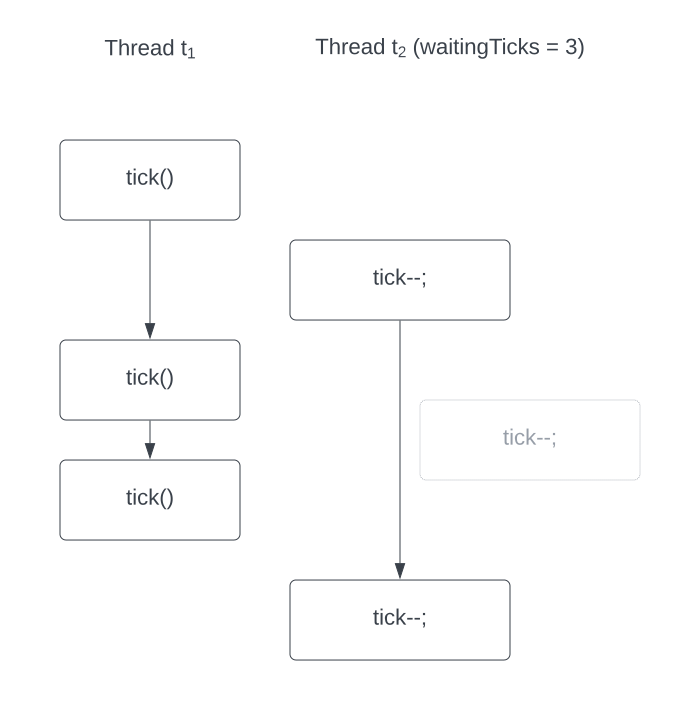
\includegraphics[scale=0.5]{chapters/Anhang/Klausuren/img/tick}
    \caption{Thread $t_1$ ruft 3 mal \texit{tick()} auf. Den Anforderungen nach müsste Thread $t_2$ danach aus der while-wait-Schleife herauskommen, erhält aber nicht die Sperre auf das Objekt von LogicalTime, um seinen eigenen Zähler rechtzeitig zu erniedrigen, bevor $t_1$ erneut \textit{tick()} aufruft. (Quelle: eigene)}
    \label{fig:tick}
\end{figure}

\section{Aufgabe 6}
Auch hier gilt, dass die Aufgabenstellung aufmerksam zu lesen ist.\\
Der Kreis soll erst ausgefüllt werden, wenn die Maustaste gelöst wird.

\begin{minted}[mathescape,
    linenos,
    numbersep=5pt,
    gobble=2,
    frame=lines,
    framesep=2mm]{java}
    private void mousePressed(double x, double y) {
        c = new Circle();
        c.setCenterX(x);
        c.setCenterY(y);
        c.setStroke(Color.RED);
        c.setFill(null); // oder Color.TRANSPARENT
        c.setRadius(RADIUS);
        graphicsPane.getChildren().add(c);
    }

    private void mouseReleased() {
        c.setFill(Color.RED);
        c = null;
    }
\end{minted}

\section{Aufgabe 8}

In der Abbildung \ref{fig:batchmodus} ist links der sequentielle Modus dargestellt, bei dem nach dem Senden einer Nachricht auf die Antwort des Servers gewartet wird, bevor eine neue Nachricht geschickt wird.
Dies wird i.d.R. verwendet, wenn das Senden einer neuen Nachricht abhängig ist von einem Ergebnis, die über die Server-Antwort übermittelt wird, oder wenn mit dem Server interagiert wird (Request abhängig vom Response).\\
Der Batch-Modus auf der rechten Seite der gleichen Abbildung ist schneller, da zwischen dem Senden von Nachrichten nicht auf Antworten gewartet werden müssen. \\
Erst nach dem Senden eine Batches von Nachrichten werden die dem Client zur Verfügung stehenden Antworten ausgelesen.\\

\noindent
In dieser Form des Batch-Modus besteht allerdings die Gefahr, dass es zu Verklemmungen kommt:
\begin{itemize}
    \item Bei dem Client kommen viele Nachrichten an, während er noch sendet.
    \item Die ankommenden Nachrichten für den Client werden gepuffert, bis sie ausgelesen werden (TCP- / OS-seitig).
    \item Läuft der Puffer voll, sorgt die Flusskontrolle (TCP) dafür, dass dem Sender mitgeteilt wird, dass keine Nachrichten mehr empfangen werden können, der Server sendet nicht mehr.
    \item Die zu sendenden Nachrichten des Servers werden in einen Puffer geschrieben.
    \item Der Sende-Puffer des Senders läuft voll.
    \item Bei dem nächsten Sende-Aufruf blockiert der Server, empfangene Nachrichten landen im Empfangspuffer
    \item Der Empfangspuffer des Servers läuft voll, der Client buffert die zu sendenden Nachrichten.
    \item Beide Anwendungen blockieren.
\end{itemize}

\\noindent
Um dieses Problem beim Batch-Modus zu umgehen, werden für das Senden und Empfangen zwei Threads auf Client-Seite erstellt: Ein Thread sendet, ein Thread empfängt. \\
Dadurch kann von dem Client immer wieder sein Empfangspuffer geleert werden, der Server wird beim Senden nicht blockiert.

\begin{figure}
    \centering
    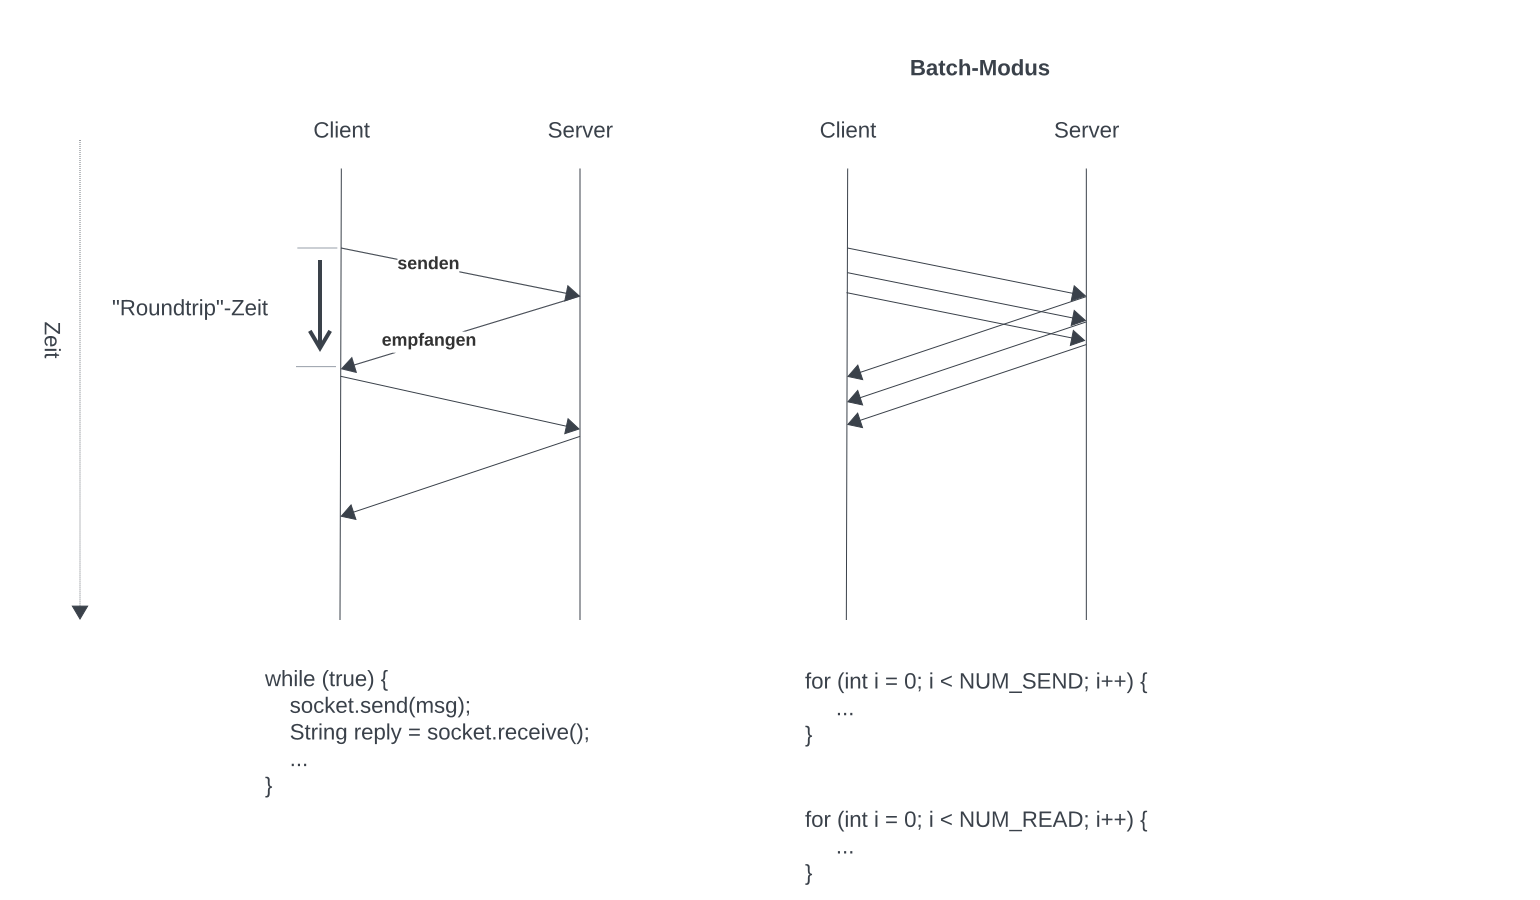
\includegraphics[scale=0.4]{chapters/Anhang/Klausuren/img/batchmodus}
    \caption{Vereinfachte Darstellung sequentieller Kommunikation und Batch-Modus (Quelle: eigene)}
    \label{fig:batchmodus}
\end{figure}
    
\begin{appendices}
    
\begin{appendices}
    \input{chapters/Anhang/Zusatzaufgaben/index}
    \input{chapters/Anhang/Klausuren/ws13}
    \input{chapters/Anhang/Klausuren/ws15-16}
    \input{chapters/Anhang/Klausuren/ws16-17}
    \input{chapters/Anhang/Klausuren/ss19}
    \input{chapters/Anhang/Präsenzphase/index}

\end{appendices}

    \chapter{WS13}\label{ch:klausurws13}

\section{Aufgabe 1}
\subsection{Lösungsvorschlag}


\begin{minted}[mathescape,
    linenos,
    numbersep=5pt,
    gobble=2,
    fontsize=\small,
    frame=lines,
    framesep=2mm]{java}
    class Zahlenschloss {

        private int[] kombination;

        private int[] state;

        private boolean opened = false;

        public Zahlenschloss(int[] kombination) {
            this.kombination = kombination;
            this.state = new int[kombination.length];
        }

        public int anzahlRaedchen() {
            return kombination.length;
        }

        public synchronized int lesen(int radnummer) {
            return state[radnummer];
        }

        public synchronized void drehen(int radnummer, int zahl) {

            state[radnummer] = zahl;
            opened = true;
            for (int i = 0; i < anzahlRaedchen(); i++) {
                if (lesen(i) != kombination[i]) {
                    opened = false;
                    break;
                }
            }

            if (opened) {
                this.notify();
            }
        }

        public synchronized void warten() {

            while (!opened) {
                try {
                    this.wait();
                } catch (InterruptedException ignored) {}
            }
        }
    }
\end{minted}\\


\subsection{Anmerkung und Ergänzungen}

\begin{itemize}
    \item Es wird eine Wartebedingung benötigt, und zwar für die Methode \code{warten()}; ankommende Threads werden
    in die Warteschlange des Zahlenschloss-Objektes geschickt, wenn \code{opened} auf false gesetzt ist, ansonsten
    verlassen diese direkt die Methode wieder.\\
    Die Methode \code{drehen} benötigt keine separate Wartebedingung.
    Es reicht aus, sicherzustellen, dass das Zahlenschloss nicht gleichzeitig von anderen Threads benutzt werden kann:
    Die Methode \code{drehen} ist hierfür synchronisiert, damit das Zahlenschloss {insg.} immer nur eine Zustandsänderung
    erfährt - es sind andere Implementierungen möglich, in denen das Zahlenschloss dann von mehreren Threads gleichzeitig
    genutzt werden darf, wenn sich die Zugriffe anhand der ``Ziel``-\code{radnummer} unterscheiden, {bspw.} durch Mutex-Semaphore,
    die pro Radnummer verwendet werden\footnote{
        der gleichzeitige Zugriff auf unterschiedliche Arrays-Indizes ist erlaubt, s. `´17.4.1. Shared Variables``: \url{https://docs.oracle.com/javase/specs/jls/se21/html/jls-17.html#jls-1.4.1} - abgerufen 14.2.2024
    }.
    \item Es gibt nur eine Wartebedingung, von daher sollte \code{notify()} genügen.\\
    Wenn wir allerdings davon ausgehen, dass mehrere Threads über die Methode \code{warten()} in die Warteschlange des Objektes eingereiht worden sind,  sollte \code{notifyAll()} verwendet werden (siehe hierzu auch Abschnitt \ref{subsec:notifyAll}).
    Dennoch ist nicht garantiert, dass auch alle Threads aus der Warteschlange gelangen, denn es kann sein, dass ein anderer Thread die Methode \code{drehen()} betritt, dort die
    Zahlenkombination ändert und \code{opened} wieder auf \code{false} gesetzt wird. \\
    Ein anderer Thread, der nun in  \code{warten()} an die Reihe kommt, überprüft die Wartebedingung, und wird wieder in die Warteschlange eingereiht.
    Es ist also durchaus möglich, dass ein Thread nicht mehr aus der Methode \code{warten()} herauskommt.\\
    Dies könnte bspw. dadurch verhindert werden, dass die Threads in eine Queue gepackt werden, und in \code{drehen()} eine Wartebedingung eingefügt wird, die erst erfüllt ist,
    wenn die Queue geleert wurde oder aus ihr entnommen wurde, in der Reihenfolge, in der die Threads in die Queue eingereiht worden sind (\textit{FIFO}) (s. a. Abschnitt~\ref{subsec:readerwriterproblem}).
    \item Bei der Teilaufgabe mit der Schleife muss die komplette Schleife synchronisiert werden, was man durch ein \code{synchronized}-Statement erreicht\footnote{siehe Abschnitt~\ref{subsec:synchronizedstatement}.}
    \begin{minted}[mathescape,
        linenos,
        numbersep=5pt,
        gobble=2,
        fontsize=\small,
        frame=lines,
        framesep=2mm]{java}
        synchronized (zk) {
            for (int i = 0; i < anzahlRaedchen; i++) {
                System.out.println(zk.lesen(i));
            }
        }
    \end{minted}
    Ansonsten läuft man Gefahr, dass sich nach Auslesen der 1. Position der Wert von Position 2 geändert hat und dadurch eine
    Zahlenkombination ausgegeben wird, die es nicht gegeben hat:
    \begin{enumerate}
        \item $K\coloneqq[0, 0, 0]$
        \item Position $K_0$ wird ausgelesen und liefert $0$.
        \item Thread ändert $K_0$ zu $1$ $\implies K\coloneqq[1, 0, 0] $.
        \item Thread ändert $K_1$ zu $2$ $\implies K\coloneqq[1, 2, 0] $.
        \item Thread ändert $K_2$ zu $3$ $\implies K\coloneqq[1, 2, 3] $.
        \item Positionen $K_1$ und $K_2$ werden ausgelesen und liefern: $2, 3$
        \item Ausgabe: $0, 2, 3$ - diese Kombination hat es in dem Fall aber tatsächlich nicht gegeben.
    \end{enumerate}
\end{itemize}

\begin{tcolorbox}[colback=red!20,color=white,title=Anmerkung]
    Die Methode \code{lesen()} als \code{synchronized} zu markieren könnte man sich vlt. sparen, wenn man davon ausgeht,
    dass die Methode ohnehin in einem \code{synchronized}-Statement verwendet wird, um alle Rädchen abzulesen.\\
    Mehrere Threads können also nicht parallel auf unterschiedliche Positionen des Feldes zugreifen, wenn die Methode
    synchronisiert ist.\\
    Allerdings ist sowohl das Skript als auch das Buch recht klar, was in dieser Situation geschehen muss (s. Skript Fopt1/2, S. 9, außerdem \cite[31, Abschnitt 2.3.6]{Oec22}): Es muss (in diesem Kurs) immer \code{synchronized} verwendet werden, wenn gleichzeitig
    Daten geschrieben und gleichzeitig diese Daten gelesen werden sollen - und eine andere Implementierung, bei der die
    einzelnen Positionen ``gelocked`` sind, so dass ein gleichzeitiger Zugriff auf unterschiedliche Rädchen möglich ist, war nicht gefordert.\\
    Ggfl. würde in anderen Implementierungen der Einsatz von \code{AtomicReferenceArray}\footnote{s. \cite[157 ff.]{Oec22}
    s. ``Class AtomicReferenceArray<E>``: \url{https://docs.oracle.com/en/java/javase/21/docs/api/java.base/java/util/concurrent/atomic/AtomicReferenceArray.html} - abgerufen 15.2.2024
    } Sinn machen, aber das Lehrmaterial ist bereits sehr eindeutig bzgl. der Verwendung von \code{synchronized}.
\end{tcolorbox}



\section{Aufgabe 3}
\subsection{Lösungsvorschlag}

\subsection*{Statische Parallelität}
Statische Parallelität erlaubt es einem Server, eine \textit{fixe} Anzahl von Verbindungen gleichzeitig zu bedienen.\\
Hierbei wird ein Feld von Threads erstellt, wobei jeder Thread das \code{ServerSocket}-Objekt als Referenz übergeben bekommt.
In der \code{run()}-Methode wird dann über \code{accept()} in einer Endlosschleife auf eingehende Verbindungen gewartet, die dann so lange bedient werden, bis sich ein Client wieder abmeldet (oder eine andere Abbruchbedingung erfüllt ist, wie z.B. ein \code{SocketTimeout}).\\
Das sich ein Client abmeldet, bekommt man bspw. dadurch mit, dass \code{null} beim Lesen von einer Nachricht des Clients zurückgegeben wird (vgl. \cite[286]{Oec22}. \\
Siehe Abschnitt~\ref{sec:seqparserver} für ein Implementierungsbeispiel.



\subsection*{Dynamische Parallelität}

Bei der \textbf{Dynamischer Parallelität} erzeugt der Server für jede Verbindung einen neuen Thread, der so lange läuft, bis der Client die Verbindung wieder trennt.\\
Die Anzahl der Threads ändert sich dadurch laufend.\\
Wird die max. Anzahl erlaubter Threads nicht kontrolliert, kann es zu einer Überlastung des Server-Rechners kommen (bspw. durch einen Denial-of-Service-Angriff.)\\

\noindent
I.d.R. ist eine Mischform aus beidem geeignet, um mehrere Clients gleichzeitig bedienen zu können, und dabei nicht Gefahr zu laufen, durch dynamisches, unbegrenztes Wachstum der Anzahl der Threads überlastet zu werden.

    \chapter{WS13}\label{ch:klausurws5-16}

\section{Rechteck-Scroll (SS15 Aufgabe 2)}

Aufgabenstellung unklar.\\
Mögliche Implementierung unter \url{https://github.com/ThorstenSuckow/fopt/tree/main/src/main/java/klausurvorbereitung/foptws1516/MouseDragsSquareDemo}.

\section{Rechteck-Scroll (WS15/16 Aufgabe 1)}

Aufgabenstellung unklar.\\
Mögliche Implementierung unter \url{https://github.com/ThorstenSuckow/fopt/tree/main/src/main/java/klausurvorbereitung/foptws1516/MaxWeightDemo}.\\

\noindent
Es gibt nur eine Warteschlange für Threads in \code{use()}, es gibt keine Wartebedingung in \code{dontUse()} und damit auch keine weitere Warteschlange.\\
Es sind durch die Zugriffe auf unterschiedliche Indizes allerdings mehrere Wartebedingungen vorhanden, weshalb hab \code{notifyAll()} nutzen sollte,
sobald ein Zugriff auf ein Feld nach Aufruf von \code{dontUse} wieder möglich wird.\\
Ansonsten bestünde die Gefahr, dass bei dem Einsatz von \code{notify()} ein wartender Thread nicht geweckt wird, obwohl er weiterlaufen könnte:\\
Angenommen, das Feld $F$ hat eine Länge von $3$, das \code{maxWeight} ist mit $2$ konfiguriert.
Thread $t_1$ mit einer Laufzeit von $200\ sek$ bekommt Zugriff auf $F_0$, setzt $currentWeight$ auf $1$.\\
Thread $t_2$ mit einer Laufzeit von $1\ sek$ möchte auf $F_1$ zugreifen, setzt $currentWeight=2$ in die Warteschlange.\\
Thread $t_3$ meldet Zugriff auf $F_0$ an und gelangt in die Warteschlange.\\
Thread $t_4$ meldet Zugriff auf $F_1$ an und gelangt in die Warteschlange.\\
Thread $t_2$ ist mit der Bearbeitung von $F_1$ fertig, $currentWeight$ wird auf $1$ gesetzt, \code{notify()} wird aufgerufen.\\
Thread $t_3$ wird aus der Warteschlange geholt, kann aber nicht weiterarbeiten, da $F_0$ noch durch den länger dauernden $t_1$ blockiert ist, und kommt wieder in die Warteschlange.\\

\noindent
Offensichtlich hätte in dem Beispiel \code{notifyAll()} dazu geführt, dass auch $T_4$ seine Wartebedingung hätte überprüfen können, und hätte so Zugriff auf $F_1$ bekommen.
Stattdessen muss nun gewartet werden, bis das nächste \code{notify()} aufgerufen wird, oder ein neu ankommender Thread $F_1$ belegt.

    \chapter{WS16-17}\label{ch:klausurws16-17}

\section{Aufgabe 1}
\subsection{Lösungshinweis}

Die erste Aufgabe verdeutlicht, was bei einem \code{notifyAll()} und unsauber gesetzten Wartebedingungen passieren kann.\\
Sei folgender Quellcode gegeben:


\begin{minted}[mathescape,
    linenos,
    numbersep=5pt,
    gobble=2,
    fontsize=\small,
    frame=lines,
    framesep=2mm]{java}
    class Cond1AndCond2 {

        private boolean cond1;
        private boolean cond2;

        public synchronized void setCond1(boolean c) {
            cond1 = c;
            notifyAll();
        }

        public synchronized void setCond2(boolean c) {
            cond2 = c;
            notifyAll();
        }

        public synchronized void cond1AndCond2() {
            while(!cond1) {
                try {
                    wait();
                } catch(InterruptedException e) { }
            }

            while(!cond2) {
                try {
                    wait();
                } catch(InterruptedException e) {}
            }
            System.out.println("cond1 and cond2:" + cond1 + " " + cond2);
        }
    }
\end{minted}\\

Man sollte auf den ersten Blick meinen, dass \code{cond1} und \code{cond2} beide \code{true} sein müssen, damit die Ausgabe erfolgt.\\
Tatsächlich ist es aber so, dass es in der Methode zwei unterschiedliche Wartebedingungen gibt.\\
Die erste Wartebedingung schickt einen Thread in die Warteschlange, wenn \code{cond1 == false} gilt.\\
Setzt ein anderer Thread über \code{setCond1(true)} das Attribut entsprechend auf \code{true}, bewirkt der nachfolgende Aufruf von \code{notifyAll()}, dass alle \textit{wartenden} Threads aus der Warteschlange entfernt werden und erneut um eine Sperre des Objektes konkurrieren.\\
Erhält ein entsprechender Thread $t_w$ die Sperre auf das Objekt und kann seine \textit{while-wait-Schleife} verlassen, kann es vorkommen, dass er erneut in die Warteschlange eingereiht wird, wegen der nachfolgenden Wartebedingung \code{cond2 == false}.\\
Angenommen, ein weiterer Thread ruft nun \code{setCond2(true)} auf, und $t_w$ kommt aus der Warteschlange und konkurriert erneut und um die Sperre des Objektes, dann kann es vorkommen, das ein anderer Thread zunächst die Sperre erhält, \code{cond1} wieder auf \code{false} setzt, dann erhält $t_w$ die Sperre, überprüft die Wartebedingung \code{cond2 == false}.\\
Wegen \code{cond2} gelangt er aus der \textit{while-wait-Schleife} und die Ausgabe erfolgt - da zwischenzeitlich \code{cond1} wieder auf \code{false} gesetzt wurde, ist die erwartete Ausgabe nicht \code{true true}, sondern \code{false true} (s. Abbildung \ref{fig:cond1cond2}).\\

\begin{figure}
    \centering
    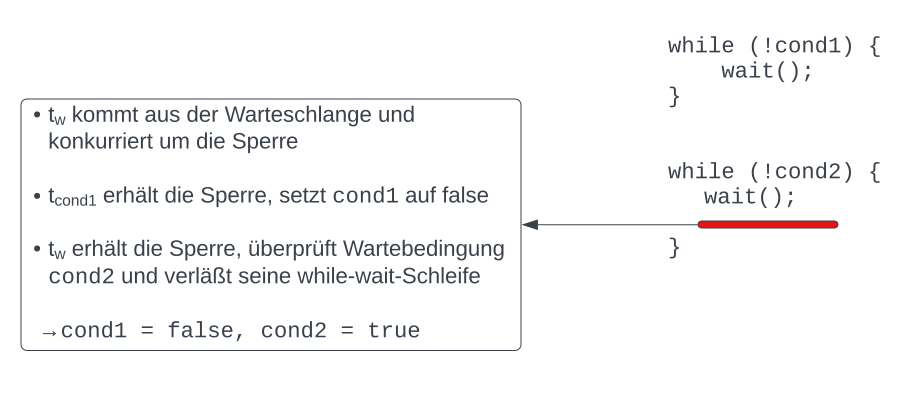
\includegraphics[scale=0.4]{chapters/Anhang/Klausuren/img/cond1cond2}
    \caption{in den rot markierten Bereich konkurriert $t_w$ um die Sperre des Objektes - wenn durch einen anderen Thread, der vor $t_w$ die Sperre erhält, \textit{cond1} auf \textit{false} gesetzt wird, stimmt die Ausgabe nicht mit der erwarteten überein. (Quelle: eigene)}
    \label{fig:cond1cond2}
\end{figure}

\noindent
Die korrekte Wartebedingung sollte lauten:

\begin{minted}[mathescape,
    linenos,
    numbersep=5pt,
    gobble=2,
    fontsize=\small,
    frame=lines,
    framesep=2mm]{java}
    public synchronized void cond1AndCond2() {
        while(!cond1 || !cond2) {
            try {
                wait();
            } catch(InterruptedException e) { }
        }
        System.out.println("cond1 and cond2:" + cond1 + " " + cond2);
    }
\end{minted}\\

Darüber hinaus müßte \code{notifyAll()} nur aufgerufen werden, wenn sowohl \code{cond1} als auch \code{cond2} auf \code{true} gesetzt sind, was leicht in den entsprechenden Methoden überprüft werden kann.
    \chapter{SS19}\label{ch:klausurss19}

\section{Aufgabe 1}

Bei der Aufgabe ist es wichtig, die Anforderungen genau zu beachten.\\
Ob eine Thread die while-wait-Schleife verlassen darf, wird von der Methode \code{tick()} gesteuert - wieviele Ticks ein Thread in der Schleife bleiben soll, wird von dem jeweiligen Thread definiert.\\
Die \code{tick()}-Methode wird von anderen Threads aufgerufen, es kann also durchaus vorkommen, dass mehrmals hintereinander
die \code{notifyAll()}-Methode aufgerufen wird - diese entfernt alle Threads aus der Warteschlange, damit die Threads ihre
Wartebedingungen erneut überprüfen können.\\
da \code{tick()} aber auch gleichzeitig einen Zähler realisieren soll, \textit{muss} es in der Methode auch eine Zählvariable geben, anhand derer die in der while-wait-Schleife enthaltenen Threads feststellen können, wie oft \code{tick()} aufgerufen wurde, um entsprechend aus der Schleife und nachfolgend der Methode herauszukommen.

\begin{figure}
    \centering
    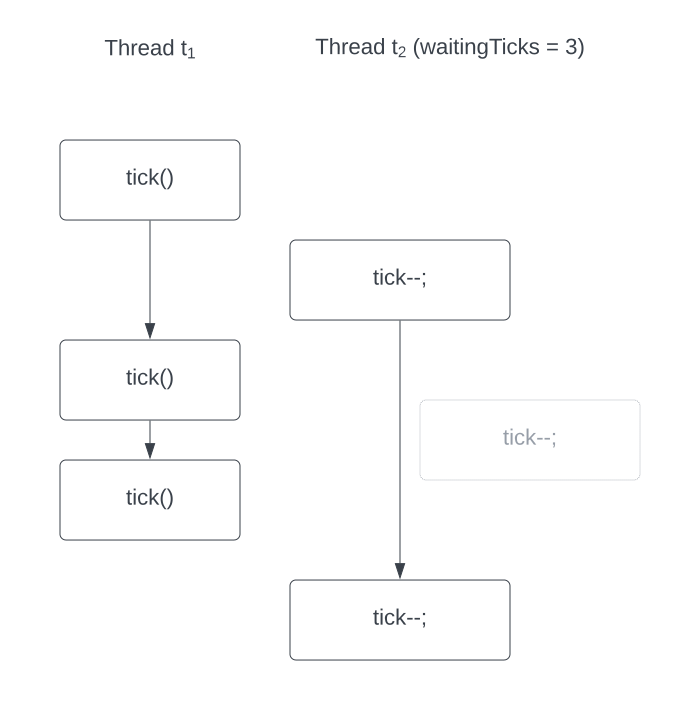
\includegraphics[scale=0.5]{chapters/Anhang/Klausuren/img/tick}
    \caption{Thread $t_1$ ruft 3 mal \texit{tick()} auf. Den Anforderungen nach müsste Thread $t_2$ danach aus der while-wait-Schleife herauskommen, erhält aber nicht die Sperre auf das Objekt von LogicalTime, um seinen eigenen Zähler rechtzeitig zu erniedrigen, bevor $t_1$ erneut \textit{tick()} aufruft. (Quelle: eigene)}
    \label{fig:tick}
\end{figure}

\section{Aufgabe 6}
Auch hier gilt, dass die Aufgabenstellung aufmerksam zu lesen ist.\\
Der Kreis soll erst ausgefüllt werden, wenn die Maustaste gelöst wird.

\begin{minted}[mathescape,
    linenos,
    numbersep=5pt,
    gobble=2,
    frame=lines,
    framesep=2mm]{java}
    private void mousePressed(double x, double y) {
        c = new Circle();
        c.setCenterX(x);
        c.setCenterY(y);
        c.setStroke(Color.RED);
        c.setFill(null); // oder Color.TRANSPARENT
        c.setRadius(RADIUS);
        graphicsPane.getChildren().add(c);
    }

    private void mouseReleased() {
        c.setFill(Color.RED);
        c = null;
    }
\end{minted}

\section{Aufgabe 8}

In der Abbildung \ref{fig:batchmodus} ist links der sequentielle Modus dargestellt, bei dem nach dem Senden einer Nachricht auf die Antwort des Servers gewartet wird, bevor eine neue Nachricht geschickt wird.
Dies wird i.d.R. verwendet, wenn das Senden einer neuen Nachricht abhängig ist von einem Ergebnis, die über die Server-Antwort übermittelt wird, oder wenn mit dem Server interagiert wird (Request abhängig vom Response).\\
Der Batch-Modus auf der rechten Seite der gleichen Abbildung ist schneller, da zwischen dem Senden von Nachrichten nicht auf Antworten gewartet werden müssen. \\
Erst nach dem Senden eine Batches von Nachrichten werden die dem Client zur Verfügung stehenden Antworten ausgelesen.\\

\noindent
In dieser Form des Batch-Modus besteht allerdings die Gefahr, dass es zu Verklemmungen kommt:
\begin{itemize}
    \item Bei dem Client kommen viele Nachrichten an, während er noch sendet.
    \item Die ankommenden Nachrichten für den Client werden gepuffert, bis sie ausgelesen werden (TCP- / OS-seitig).
    \item Läuft der Puffer voll, sorgt die Flusskontrolle (TCP) dafür, dass dem Sender mitgeteilt wird, dass keine Nachrichten mehr empfangen werden können, der Server sendet nicht mehr.
    \item Die zu sendenden Nachrichten des Servers werden in einen Puffer geschrieben.
    \item Der Sende-Puffer des Senders läuft voll.
    \item Bei dem nächsten Sende-Aufruf blockiert der Server, empfangene Nachrichten landen im Empfangspuffer
    \item Der Empfangspuffer des Servers läuft voll, der Client buffert die zu sendenden Nachrichten.
    \item Beide Anwendungen blockieren.
\end{itemize}

\\noindent
Um dieses Problem beim Batch-Modus zu umgehen, werden für das Senden und Empfangen zwei Threads auf Client-Seite erstellt: Ein Thread sendet, ein Thread empfängt. \\
Dadurch kann von dem Client immer wieder sein Empfangspuffer geleert werden, der Server wird beim Senden nicht blockiert.

\begin{figure}
    \centering
    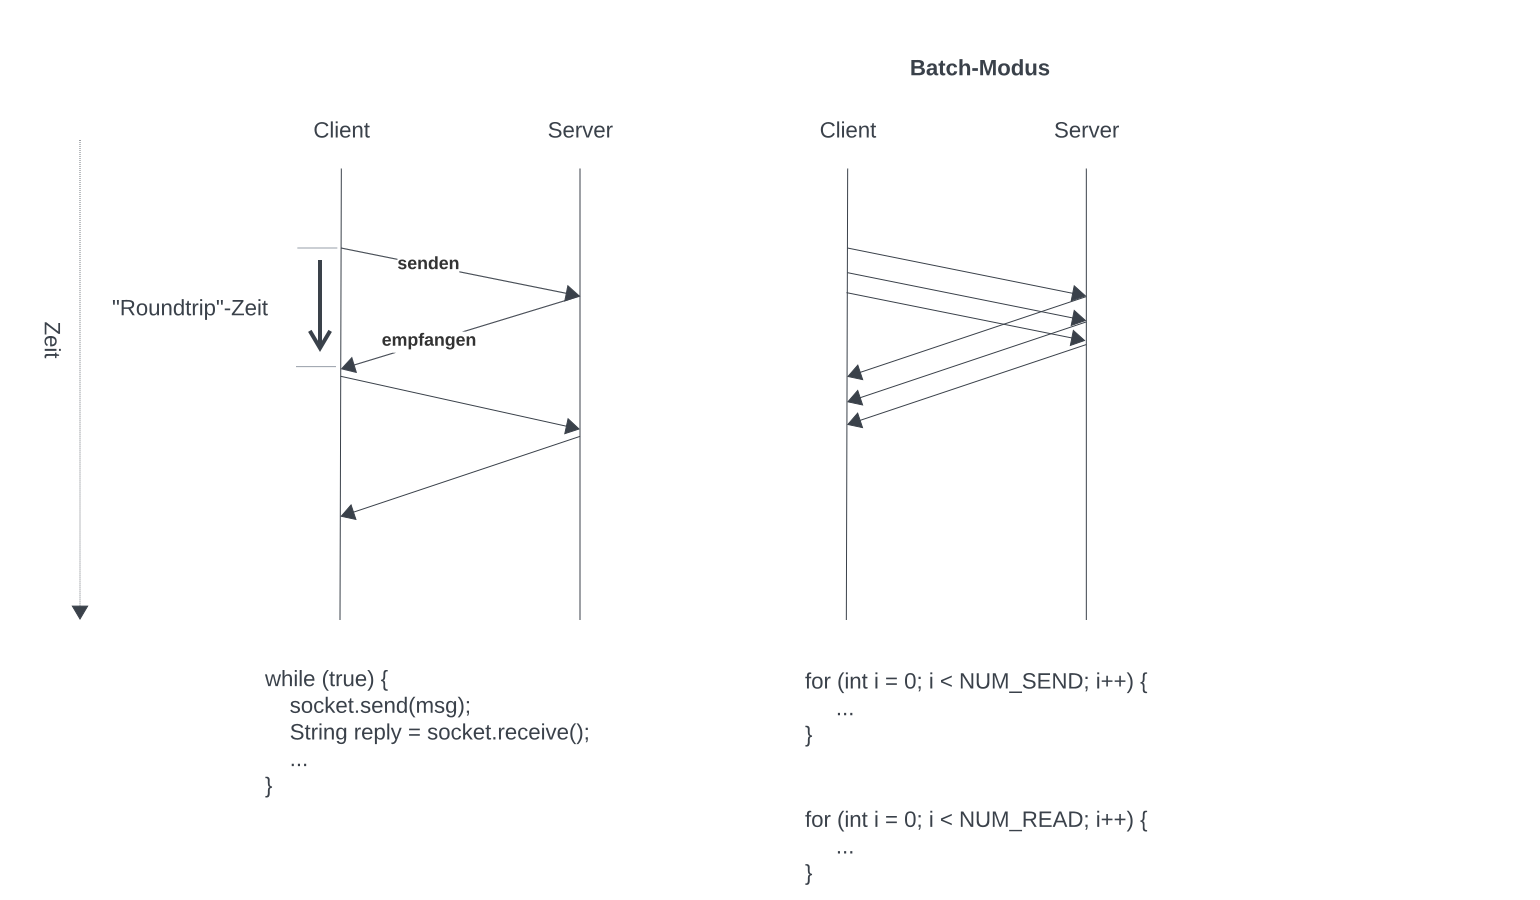
\includegraphics[scale=0.4]{chapters/Anhang/Klausuren/img/batchmodus}
    \caption{Vereinfachte Darstellung sequentieller Kommunikation und Batch-Modus (Quelle: eigene)}
    \label{fig:batchmodus}
\end{figure}
    
\begin{appendices}
    \input{chapters/Anhang/Zusatzaufgaben/index}
    \input{chapters/Anhang/Klausuren/ws13}
    \input{chapters/Anhang/Klausuren/ws15-16}
    \input{chapters/Anhang/Klausuren/ws16-17}
    \input{chapters/Anhang/Klausuren/ss19}
    \input{chapters/Anhang/Präsenzphase/index}

\end{appendices}


\end{appendices}


\end{appendices}



\begin{appendices}
    
\begin{appendices}
    
\begin{appendices}
    \input{chapters/Anhang/Zusatzaufgaben/index}
    \input{chapters/Anhang/Klausuren/ws13}
    \input{chapters/Anhang/Klausuren/ws15-16}
    \input{chapters/Anhang/Klausuren/ws16-17}
    \input{chapters/Anhang/Klausuren/ss19}
    \input{chapters/Anhang/Präsenzphase/index}

\end{appendices}

    \chapter{WS13}\label{ch:klausurws13}

\section{Aufgabe 1}
\subsection{Lösungsvorschlag}


\begin{minted}[mathescape,
    linenos,
    numbersep=5pt,
    gobble=2,
    fontsize=\small,
    frame=lines,
    framesep=2mm]{java}
    class Zahlenschloss {

        private int[] kombination;

        private int[] state;

        private boolean opened = false;

        public Zahlenschloss(int[] kombination) {
            this.kombination = kombination;
            this.state = new int[kombination.length];
        }

        public int anzahlRaedchen() {
            return kombination.length;
        }

        public synchronized int lesen(int radnummer) {
            return state[radnummer];
        }

        public synchronized void drehen(int radnummer, int zahl) {

            state[radnummer] = zahl;
            opened = true;
            for (int i = 0; i < anzahlRaedchen(); i++) {
                if (lesen(i) != kombination[i]) {
                    opened = false;
                    break;
                }
            }

            if (opened) {
                this.notify();
            }
        }

        public synchronized void warten() {

            while (!opened) {
                try {
                    this.wait();
                } catch (InterruptedException ignored) {}
            }
        }
    }
\end{minted}\\


\subsection{Anmerkung und Ergänzungen}

\begin{itemize}
    \item Es wird eine Wartebedingung benötigt, und zwar für die Methode \code{warten()}; ankommende Threads werden
    in die Warteschlange des Zahlenschloss-Objektes geschickt, wenn \code{opened} auf false gesetzt ist, ansonsten
    verlassen diese direkt die Methode wieder.\\
    Die Methode \code{drehen} benötigt keine separate Wartebedingung.
    Es reicht aus, sicherzustellen, dass das Zahlenschloss nicht gleichzeitig von anderen Threads benutzt werden kann:
    Die Methode \code{drehen} ist hierfür synchronisiert, damit das Zahlenschloss {insg.} immer nur eine Zustandsänderung
    erfährt - es sind andere Implementierungen möglich, in denen das Zahlenschloss dann von mehreren Threads gleichzeitig
    genutzt werden darf, wenn sich die Zugriffe anhand der ``Ziel``-\code{radnummer} unterscheiden, {bspw.} durch Mutex-Semaphore,
    die pro Radnummer verwendet werden\footnote{
        der gleichzeitige Zugriff auf unterschiedliche Arrays-Indizes ist erlaubt, s. `´17.4.1. Shared Variables``: \url{https://docs.oracle.com/javase/specs/jls/se21/html/jls-17.html#jls-1.4.1} - abgerufen 14.2.2024
    }.
    \item Es gibt nur eine Wartebedingung, von daher sollte \code{notify()} genügen.\\
    Wenn wir allerdings davon ausgehen, dass mehrere Threads über die Methode \code{warten()} in die Warteschlange des Objektes eingereiht worden sind,  sollte \code{notifyAll()} verwendet werden (siehe hierzu auch Abschnitt \ref{subsec:notifyAll}).
    Dennoch ist nicht garantiert, dass auch alle Threads aus der Warteschlange gelangen, denn es kann sein, dass ein anderer Thread die Methode \code{drehen()} betritt, dort die
    Zahlenkombination ändert und \code{opened} wieder auf \code{false} gesetzt wird. \\
    Ein anderer Thread, der nun in  \code{warten()} an die Reihe kommt, überprüft die Wartebedingung, und wird wieder in die Warteschlange eingereiht.
    Es ist also durchaus möglich, dass ein Thread nicht mehr aus der Methode \code{warten()} herauskommt.\\
    Dies könnte bspw. dadurch verhindert werden, dass die Threads in eine Queue gepackt werden, und in \code{drehen()} eine Wartebedingung eingefügt wird, die erst erfüllt ist,
    wenn die Queue geleert wurde oder aus ihr entnommen wurde, in der Reihenfolge, in der die Threads in die Queue eingereiht worden sind (\textit{FIFO}) (s. a. Abschnitt~\ref{subsec:readerwriterproblem}).
    \item Bei der Teilaufgabe mit der Schleife muss die komplette Schleife synchronisiert werden, was man durch ein \code{synchronized}-Statement erreicht\footnote{siehe Abschnitt~\ref{subsec:synchronizedstatement}.}
    \begin{minted}[mathescape,
        linenos,
        numbersep=5pt,
        gobble=2,
        fontsize=\small,
        frame=lines,
        framesep=2mm]{java}
        synchronized (zk) {
            for (int i = 0; i < anzahlRaedchen; i++) {
                System.out.println(zk.lesen(i));
            }
        }
    \end{minted}
    Ansonsten läuft man Gefahr, dass sich nach Auslesen der 1. Position der Wert von Position 2 geändert hat und dadurch eine
    Zahlenkombination ausgegeben wird, die es nicht gegeben hat:
    \begin{enumerate}
        \item $K\coloneqq[0, 0, 0]$
        \item Position $K_0$ wird ausgelesen und liefert $0$.
        \item Thread ändert $K_0$ zu $1$ $\implies K\coloneqq[1, 0, 0] $.
        \item Thread ändert $K_1$ zu $2$ $\implies K\coloneqq[1, 2, 0] $.
        \item Thread ändert $K_2$ zu $3$ $\implies K\coloneqq[1, 2, 3] $.
        \item Positionen $K_1$ und $K_2$ werden ausgelesen und liefern: $2, 3$
        \item Ausgabe: $0, 2, 3$ - diese Kombination hat es in dem Fall aber tatsächlich nicht gegeben.
    \end{enumerate}
\end{itemize}

\begin{tcolorbox}[colback=red!20,color=white,title=Anmerkung]
    Die Methode \code{lesen()} als \code{synchronized} zu markieren könnte man sich vlt. sparen, wenn man davon ausgeht,
    dass die Methode ohnehin in einem \code{synchronized}-Statement verwendet wird, um alle Rädchen abzulesen.\\
    Mehrere Threads können also nicht parallel auf unterschiedliche Positionen des Feldes zugreifen, wenn die Methode
    synchronisiert ist.\\
    Allerdings ist sowohl das Skript als auch das Buch recht klar, was in dieser Situation geschehen muss (s. Skript Fopt1/2, S. 9, außerdem \cite[31, Abschnitt 2.3.6]{Oec22}): Es muss (in diesem Kurs) immer \code{synchronized} verwendet werden, wenn gleichzeitig
    Daten geschrieben und gleichzeitig diese Daten gelesen werden sollen - und eine andere Implementierung, bei der die
    einzelnen Positionen ``gelocked`` sind, so dass ein gleichzeitiger Zugriff auf unterschiedliche Rädchen möglich ist, war nicht gefordert.\\
    Ggfl. würde in anderen Implementierungen der Einsatz von \code{AtomicReferenceArray}\footnote{s. \cite[157 ff.]{Oec22}
    s. ``Class AtomicReferenceArray<E>``: \url{https://docs.oracle.com/en/java/javase/21/docs/api/java.base/java/util/concurrent/atomic/AtomicReferenceArray.html} - abgerufen 15.2.2024
    } Sinn machen, aber das Lehrmaterial ist bereits sehr eindeutig bzgl. der Verwendung von \code{synchronized}.
\end{tcolorbox}



\section{Aufgabe 3}
\subsection{Lösungsvorschlag}

\subsection*{Statische Parallelität}
Statische Parallelität erlaubt es einem Server, eine \textit{fixe} Anzahl von Verbindungen gleichzeitig zu bedienen.\\
Hierbei wird ein Feld von Threads erstellt, wobei jeder Thread das \code{ServerSocket}-Objekt als Referenz übergeben bekommt.
In der \code{run()}-Methode wird dann über \code{accept()} in einer Endlosschleife auf eingehende Verbindungen gewartet, die dann so lange bedient werden, bis sich ein Client wieder abmeldet (oder eine andere Abbruchbedingung erfüllt ist, wie z.B. ein \code{SocketTimeout}).\\
Das sich ein Client abmeldet, bekommt man bspw. dadurch mit, dass \code{null} beim Lesen von einer Nachricht des Clients zurückgegeben wird (vgl. \cite[286]{Oec22}. \\
Siehe Abschnitt~\ref{sec:seqparserver} für ein Implementierungsbeispiel.



\subsection*{Dynamische Parallelität}

Bei der \textbf{Dynamischer Parallelität} erzeugt der Server für jede Verbindung einen neuen Thread, der so lange läuft, bis der Client die Verbindung wieder trennt.\\
Die Anzahl der Threads ändert sich dadurch laufend.\\
Wird die max. Anzahl erlaubter Threads nicht kontrolliert, kann es zu einer Überlastung des Server-Rechners kommen (bspw. durch einen Denial-of-Service-Angriff.)\\

\noindent
I.d.R. ist eine Mischform aus beidem geeignet, um mehrere Clients gleichzeitig bedienen zu können, und dabei nicht Gefahr zu laufen, durch dynamisches, unbegrenztes Wachstum der Anzahl der Threads überlastet zu werden.

    \chapter{WS13}\label{ch:klausurws5-16}

\section{Rechteck-Scroll (SS15 Aufgabe 2)}

Aufgabenstellung unklar.\\
Mögliche Implementierung unter \url{https://github.com/ThorstenSuckow/fopt/tree/main/src/main/java/klausurvorbereitung/foptws1516/MouseDragsSquareDemo}.

\section{Rechteck-Scroll (WS15/16 Aufgabe 1)}

Aufgabenstellung unklar.\\
Mögliche Implementierung unter \url{https://github.com/ThorstenSuckow/fopt/tree/main/src/main/java/klausurvorbereitung/foptws1516/MaxWeightDemo}.\\

\noindent
Es gibt nur eine Warteschlange für Threads in \code{use()}, es gibt keine Wartebedingung in \code{dontUse()} und damit auch keine weitere Warteschlange.\\
Es sind durch die Zugriffe auf unterschiedliche Indizes allerdings mehrere Wartebedingungen vorhanden, weshalb hab \code{notifyAll()} nutzen sollte,
sobald ein Zugriff auf ein Feld nach Aufruf von \code{dontUse} wieder möglich wird.\\
Ansonsten bestünde die Gefahr, dass bei dem Einsatz von \code{notify()} ein wartender Thread nicht geweckt wird, obwohl er weiterlaufen könnte:\\
Angenommen, das Feld $F$ hat eine Länge von $3$, das \code{maxWeight} ist mit $2$ konfiguriert.
Thread $t_1$ mit einer Laufzeit von $200\ sek$ bekommt Zugriff auf $F_0$, setzt $currentWeight$ auf $1$.\\
Thread $t_2$ mit einer Laufzeit von $1\ sek$ möchte auf $F_1$ zugreifen, setzt $currentWeight=2$ in die Warteschlange.\\
Thread $t_3$ meldet Zugriff auf $F_0$ an und gelangt in die Warteschlange.\\
Thread $t_4$ meldet Zugriff auf $F_1$ an und gelangt in die Warteschlange.\\
Thread $t_2$ ist mit der Bearbeitung von $F_1$ fertig, $currentWeight$ wird auf $1$ gesetzt, \code{notify()} wird aufgerufen.\\
Thread $t_3$ wird aus der Warteschlange geholt, kann aber nicht weiterarbeiten, da $F_0$ noch durch den länger dauernden $t_1$ blockiert ist, und kommt wieder in die Warteschlange.\\

\noindent
Offensichtlich hätte in dem Beispiel \code{notifyAll()} dazu geführt, dass auch $T_4$ seine Wartebedingung hätte überprüfen können, und hätte so Zugriff auf $F_1$ bekommen.
Stattdessen muss nun gewartet werden, bis das nächste \code{notify()} aufgerufen wird, oder ein neu ankommender Thread $F_1$ belegt.

    \chapter{WS16-17}\label{ch:klausurws16-17}

\section{Aufgabe 1}
\subsection{Lösungshinweis}

Die erste Aufgabe verdeutlicht, was bei einem \code{notifyAll()} und unsauber gesetzten Wartebedingungen passieren kann.\\
Sei folgender Quellcode gegeben:


\begin{minted}[mathescape,
    linenos,
    numbersep=5pt,
    gobble=2,
    fontsize=\small,
    frame=lines,
    framesep=2mm]{java}
    class Cond1AndCond2 {

        private boolean cond1;
        private boolean cond2;

        public synchronized void setCond1(boolean c) {
            cond1 = c;
            notifyAll();
        }

        public synchronized void setCond2(boolean c) {
            cond2 = c;
            notifyAll();
        }

        public synchronized void cond1AndCond2() {
            while(!cond1) {
                try {
                    wait();
                } catch(InterruptedException e) { }
            }

            while(!cond2) {
                try {
                    wait();
                } catch(InterruptedException e) {}
            }
            System.out.println("cond1 and cond2:" + cond1 + " " + cond2);
        }
    }
\end{minted}\\

Man sollte auf den ersten Blick meinen, dass \code{cond1} und \code{cond2} beide \code{true} sein müssen, damit die Ausgabe erfolgt.\\
Tatsächlich ist es aber so, dass es in der Methode zwei unterschiedliche Wartebedingungen gibt.\\
Die erste Wartebedingung schickt einen Thread in die Warteschlange, wenn \code{cond1 == false} gilt.\\
Setzt ein anderer Thread über \code{setCond1(true)} das Attribut entsprechend auf \code{true}, bewirkt der nachfolgende Aufruf von \code{notifyAll()}, dass alle \textit{wartenden} Threads aus der Warteschlange entfernt werden und erneut um eine Sperre des Objektes konkurrieren.\\
Erhält ein entsprechender Thread $t_w$ die Sperre auf das Objekt und kann seine \textit{while-wait-Schleife} verlassen, kann es vorkommen, dass er erneut in die Warteschlange eingereiht wird, wegen der nachfolgenden Wartebedingung \code{cond2 == false}.\\
Angenommen, ein weiterer Thread ruft nun \code{setCond2(true)} auf, und $t_w$ kommt aus der Warteschlange und konkurriert erneut und um die Sperre des Objektes, dann kann es vorkommen, das ein anderer Thread zunächst die Sperre erhält, \code{cond1} wieder auf \code{false} setzt, dann erhält $t_w$ die Sperre, überprüft die Wartebedingung \code{cond2 == false}.\\
Wegen \code{cond2} gelangt er aus der \textit{while-wait-Schleife} und die Ausgabe erfolgt - da zwischenzeitlich \code{cond1} wieder auf \code{false} gesetzt wurde, ist die erwartete Ausgabe nicht \code{true true}, sondern \code{false true} (s. Abbildung \ref{fig:cond1cond2}).\\

\begin{figure}
    \centering
    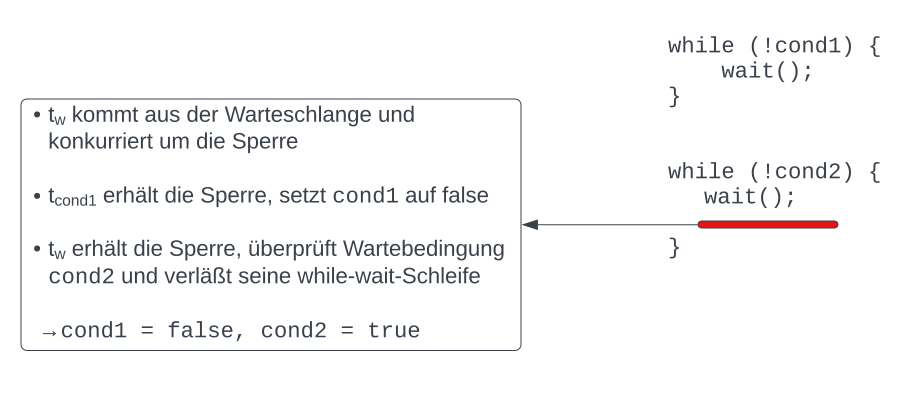
\includegraphics[scale=0.4]{chapters/Anhang/Klausuren/img/cond1cond2}
    \caption{in den rot markierten Bereich konkurriert $t_w$ um die Sperre des Objektes - wenn durch einen anderen Thread, der vor $t_w$ die Sperre erhält, \textit{cond1} auf \textit{false} gesetzt wird, stimmt die Ausgabe nicht mit der erwarteten überein. (Quelle: eigene)}
    \label{fig:cond1cond2}
\end{figure}

\noindent
Die korrekte Wartebedingung sollte lauten:

\begin{minted}[mathescape,
    linenos,
    numbersep=5pt,
    gobble=2,
    fontsize=\small,
    frame=lines,
    framesep=2mm]{java}
    public synchronized void cond1AndCond2() {
        while(!cond1 || !cond2) {
            try {
                wait();
            } catch(InterruptedException e) { }
        }
        System.out.println("cond1 and cond2:" + cond1 + " " + cond2);
    }
\end{minted}\\

Darüber hinaus müßte \code{notifyAll()} nur aufgerufen werden, wenn sowohl \code{cond1} als auch \code{cond2} auf \code{true} gesetzt sind, was leicht in den entsprechenden Methoden überprüft werden kann.
    \chapter{SS19}\label{ch:klausurss19}

\section{Aufgabe 1}

Bei der Aufgabe ist es wichtig, die Anforderungen genau zu beachten.\\
Ob eine Thread die while-wait-Schleife verlassen darf, wird von der Methode \code{tick()} gesteuert - wieviele Ticks ein Thread in der Schleife bleiben soll, wird von dem jeweiligen Thread definiert.\\
Die \code{tick()}-Methode wird von anderen Threads aufgerufen, es kann also durchaus vorkommen, dass mehrmals hintereinander
die \code{notifyAll()}-Methode aufgerufen wird - diese entfernt alle Threads aus der Warteschlange, damit die Threads ihre
Wartebedingungen erneut überprüfen können.\\
da \code{tick()} aber auch gleichzeitig einen Zähler realisieren soll, \textit{muss} es in der Methode auch eine Zählvariable geben, anhand derer die in der while-wait-Schleife enthaltenen Threads feststellen können, wie oft \code{tick()} aufgerufen wurde, um entsprechend aus der Schleife und nachfolgend der Methode herauszukommen.

\begin{figure}
    \centering
    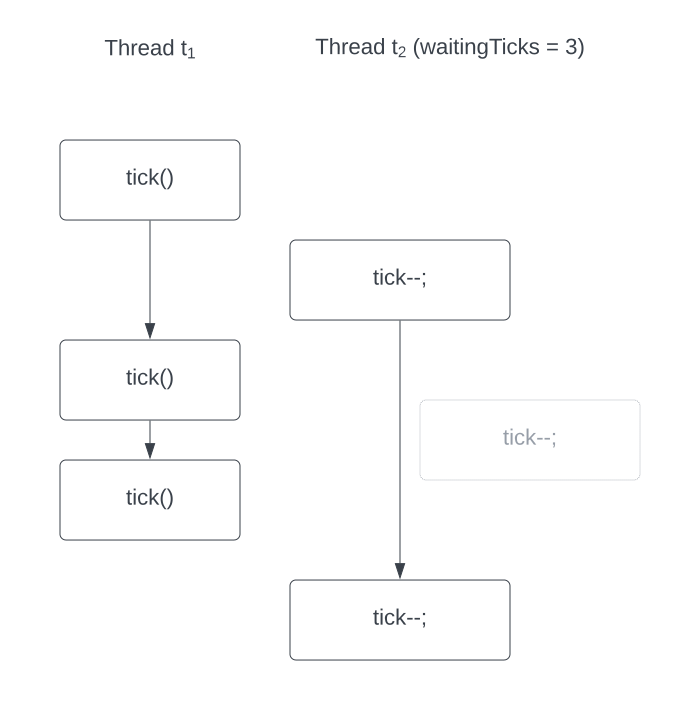
\includegraphics[scale=0.5]{chapters/Anhang/Klausuren/img/tick}
    \caption{Thread $t_1$ ruft 3 mal \texit{tick()} auf. Den Anforderungen nach müsste Thread $t_2$ danach aus der while-wait-Schleife herauskommen, erhält aber nicht die Sperre auf das Objekt von LogicalTime, um seinen eigenen Zähler rechtzeitig zu erniedrigen, bevor $t_1$ erneut \textit{tick()} aufruft. (Quelle: eigene)}
    \label{fig:tick}
\end{figure}

\section{Aufgabe 6}
Auch hier gilt, dass die Aufgabenstellung aufmerksam zu lesen ist.\\
Der Kreis soll erst ausgefüllt werden, wenn die Maustaste gelöst wird.

\begin{minted}[mathescape,
    linenos,
    numbersep=5pt,
    gobble=2,
    frame=lines,
    framesep=2mm]{java}
    private void mousePressed(double x, double y) {
        c = new Circle();
        c.setCenterX(x);
        c.setCenterY(y);
        c.setStroke(Color.RED);
        c.setFill(null); // oder Color.TRANSPARENT
        c.setRadius(RADIUS);
        graphicsPane.getChildren().add(c);
    }

    private void mouseReleased() {
        c.setFill(Color.RED);
        c = null;
    }
\end{minted}

\section{Aufgabe 8}

In der Abbildung \ref{fig:batchmodus} ist links der sequentielle Modus dargestellt, bei dem nach dem Senden einer Nachricht auf die Antwort des Servers gewartet wird, bevor eine neue Nachricht geschickt wird.
Dies wird i.d.R. verwendet, wenn das Senden einer neuen Nachricht abhängig ist von einem Ergebnis, die über die Server-Antwort übermittelt wird, oder wenn mit dem Server interagiert wird (Request abhängig vom Response).\\
Der Batch-Modus auf der rechten Seite der gleichen Abbildung ist schneller, da zwischen dem Senden von Nachrichten nicht auf Antworten gewartet werden müssen. \\
Erst nach dem Senden eine Batches von Nachrichten werden die dem Client zur Verfügung stehenden Antworten ausgelesen.\\

\noindent
In dieser Form des Batch-Modus besteht allerdings die Gefahr, dass es zu Verklemmungen kommt:
\begin{itemize}
    \item Bei dem Client kommen viele Nachrichten an, während er noch sendet.
    \item Die ankommenden Nachrichten für den Client werden gepuffert, bis sie ausgelesen werden (TCP- / OS-seitig).
    \item Läuft der Puffer voll, sorgt die Flusskontrolle (TCP) dafür, dass dem Sender mitgeteilt wird, dass keine Nachrichten mehr empfangen werden können, der Server sendet nicht mehr.
    \item Die zu sendenden Nachrichten des Servers werden in einen Puffer geschrieben.
    \item Der Sende-Puffer des Senders läuft voll.
    \item Bei dem nächsten Sende-Aufruf blockiert der Server, empfangene Nachrichten landen im Empfangspuffer
    \item Der Empfangspuffer des Servers läuft voll, der Client buffert die zu sendenden Nachrichten.
    \item Beide Anwendungen blockieren.
\end{itemize}

\\noindent
Um dieses Problem beim Batch-Modus zu umgehen, werden für das Senden und Empfangen zwei Threads auf Client-Seite erstellt: Ein Thread sendet, ein Thread empfängt. \\
Dadurch kann von dem Client immer wieder sein Empfangspuffer geleert werden, der Server wird beim Senden nicht blockiert.

\begin{figure}
    \centering
    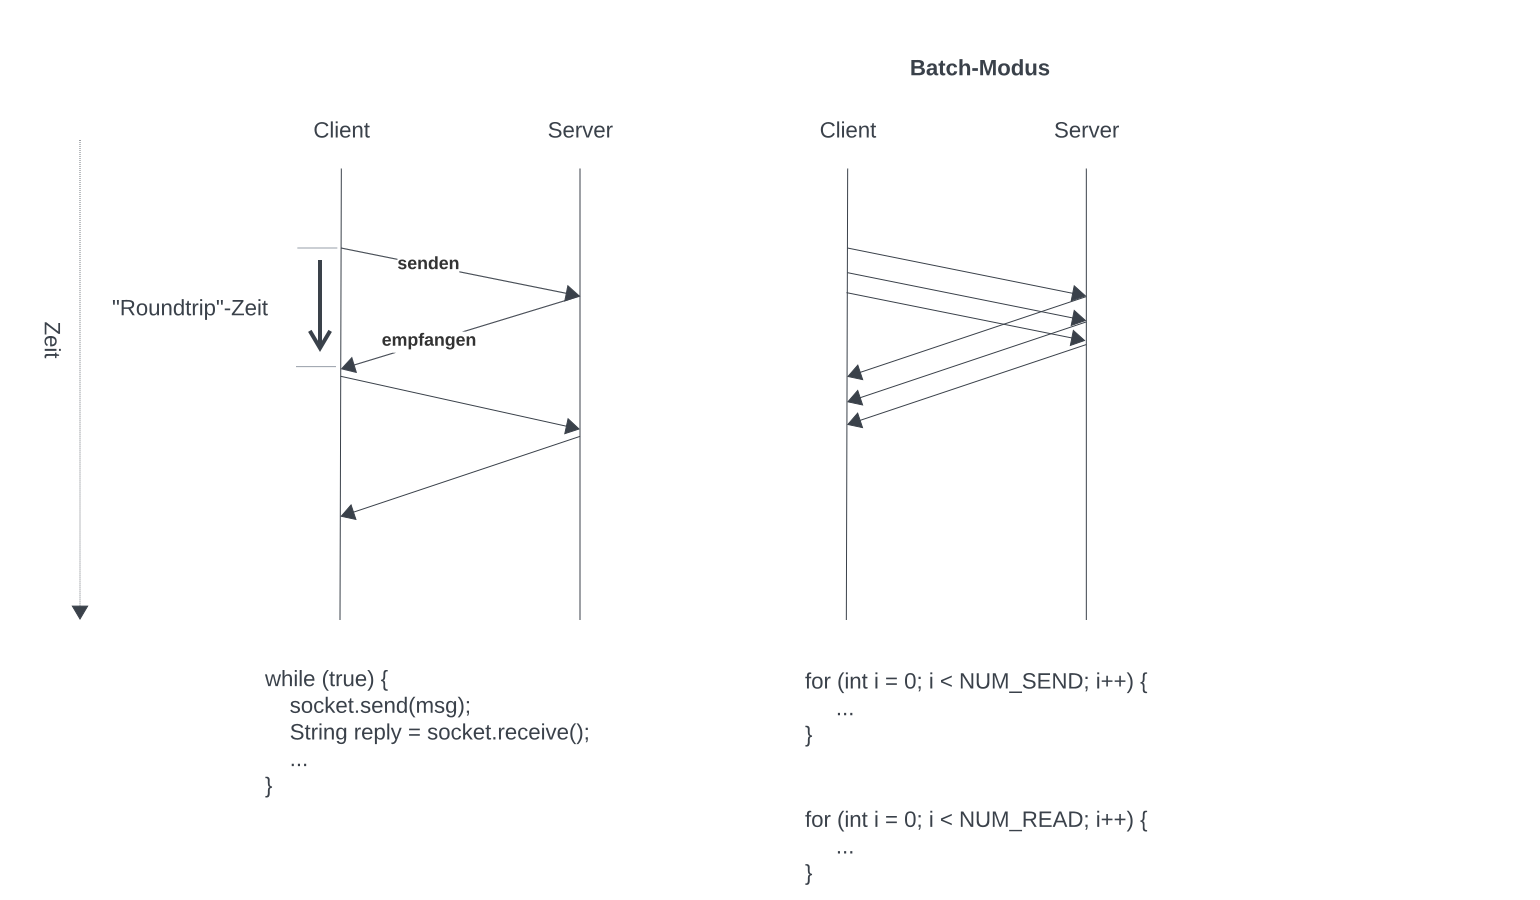
\includegraphics[scale=0.4]{chapters/Anhang/Klausuren/img/batchmodus}
    \caption{Vereinfachte Darstellung sequentieller Kommunikation und Batch-Modus (Quelle: eigene)}
    \label{fig:batchmodus}
\end{figure}
    
\begin{appendices}
    \input{chapters/Anhang/Zusatzaufgaben/index}
    \input{chapters/Anhang/Klausuren/ws13}
    \input{chapters/Anhang/Klausuren/ws15-16}
    \input{chapters/Anhang/Klausuren/ws16-17}
    \input{chapters/Anhang/Klausuren/ss19}
    \input{chapters/Anhang/Präsenzphase/index}

\end{appendices}


\end{appendices}

    \chapter{WS13}\label{ch:klausurws13}

\section{Aufgabe 1}
\subsection{Lösungsvorschlag}


\begin{minted}[mathescape,
    linenos,
    numbersep=5pt,
    gobble=2,
    fontsize=\small,
    frame=lines,
    framesep=2mm]{java}
    class Zahlenschloss {

        private int[] kombination;

        private int[] state;

        private boolean opened = false;

        public Zahlenschloss(int[] kombination) {
            this.kombination = kombination;
            this.state = new int[kombination.length];
        }

        public int anzahlRaedchen() {
            return kombination.length;
        }

        public synchronized int lesen(int radnummer) {
            return state[radnummer];
        }

        public synchronized void drehen(int radnummer, int zahl) {

            state[radnummer] = zahl;
            opened = true;
            for (int i = 0; i < anzahlRaedchen(); i++) {
                if (lesen(i) != kombination[i]) {
                    opened = false;
                    break;
                }
            }

            if (opened) {
                this.notify();
            }
        }

        public synchronized void warten() {

            while (!opened) {
                try {
                    this.wait();
                } catch (InterruptedException ignored) {}
            }
        }
    }
\end{minted}\\


\subsection{Anmerkung und Ergänzungen}

\begin{itemize}
    \item Es wird eine Wartebedingung benötigt, und zwar für die Methode \code{warten()}; ankommende Threads werden
    in die Warteschlange des Zahlenschloss-Objektes geschickt, wenn \code{opened} auf false gesetzt ist, ansonsten
    verlassen diese direkt die Methode wieder.\\
    Die Methode \code{drehen} benötigt keine separate Wartebedingung.
    Es reicht aus, sicherzustellen, dass das Zahlenschloss nicht gleichzeitig von anderen Threads benutzt werden kann:
    Die Methode \code{drehen} ist hierfür synchronisiert, damit das Zahlenschloss {insg.} immer nur eine Zustandsänderung
    erfährt - es sind andere Implementierungen möglich, in denen das Zahlenschloss dann von mehreren Threads gleichzeitig
    genutzt werden darf, wenn sich die Zugriffe anhand der ``Ziel``-\code{radnummer} unterscheiden, {bspw.} durch Mutex-Semaphore,
    die pro Radnummer verwendet werden\footnote{
        der gleichzeitige Zugriff auf unterschiedliche Arrays-Indizes ist erlaubt, s. `´17.4.1. Shared Variables``: \url{https://docs.oracle.com/javase/specs/jls/se21/html/jls-17.html#jls-1.4.1} - abgerufen 14.2.2024
    }.
    \item Es gibt nur eine Wartebedingung, von daher sollte \code{notify()} genügen.\\
    Wenn wir allerdings davon ausgehen, dass mehrere Threads über die Methode \code{warten()} in die Warteschlange des Objektes eingereiht worden sind,  sollte \code{notifyAll()} verwendet werden (siehe hierzu auch Abschnitt \ref{subsec:notifyAll}).
    Dennoch ist nicht garantiert, dass auch alle Threads aus der Warteschlange gelangen, denn es kann sein, dass ein anderer Thread die Methode \code{drehen()} betritt, dort die
    Zahlenkombination ändert und \code{opened} wieder auf \code{false} gesetzt wird. \\
    Ein anderer Thread, der nun in  \code{warten()} an die Reihe kommt, überprüft die Wartebedingung, und wird wieder in die Warteschlange eingereiht.
    Es ist also durchaus möglich, dass ein Thread nicht mehr aus der Methode \code{warten()} herauskommt.\\
    Dies könnte bspw. dadurch verhindert werden, dass die Threads in eine Queue gepackt werden, und in \code{drehen()} eine Wartebedingung eingefügt wird, die erst erfüllt ist,
    wenn die Queue geleert wurde oder aus ihr entnommen wurde, in der Reihenfolge, in der die Threads in die Queue eingereiht worden sind (\textit{FIFO}) (s. a. Abschnitt~\ref{subsec:readerwriterproblem}).
    \item Bei der Teilaufgabe mit der Schleife muss die komplette Schleife synchronisiert werden, was man durch ein \code{synchronized}-Statement erreicht\footnote{siehe Abschnitt~\ref{subsec:synchronizedstatement}.}
    \begin{minted}[mathescape,
        linenos,
        numbersep=5pt,
        gobble=2,
        fontsize=\small,
        frame=lines,
        framesep=2mm]{java}
        synchronized (zk) {
            for (int i = 0; i < anzahlRaedchen; i++) {
                System.out.println(zk.lesen(i));
            }
        }
    \end{minted}
    Ansonsten läuft man Gefahr, dass sich nach Auslesen der 1. Position der Wert von Position 2 geändert hat und dadurch eine
    Zahlenkombination ausgegeben wird, die es nicht gegeben hat:
    \begin{enumerate}
        \item $K\coloneqq[0, 0, 0]$
        \item Position $K_0$ wird ausgelesen und liefert $0$.
        \item Thread ändert $K_0$ zu $1$ $\implies K\coloneqq[1, 0, 0] $.
        \item Thread ändert $K_1$ zu $2$ $\implies K\coloneqq[1, 2, 0] $.
        \item Thread ändert $K_2$ zu $3$ $\implies K\coloneqq[1, 2, 3] $.
        \item Positionen $K_1$ und $K_2$ werden ausgelesen und liefern: $2, 3$
        \item Ausgabe: $0, 2, 3$ - diese Kombination hat es in dem Fall aber tatsächlich nicht gegeben.
    \end{enumerate}
\end{itemize}

\begin{tcolorbox}[colback=red!20,color=white,title=Anmerkung]
    Die Methode \code{lesen()} als \code{synchronized} zu markieren könnte man sich vlt. sparen, wenn man davon ausgeht,
    dass die Methode ohnehin in einem \code{synchronized}-Statement verwendet wird, um alle Rädchen abzulesen.\\
    Mehrere Threads können also nicht parallel auf unterschiedliche Positionen des Feldes zugreifen, wenn die Methode
    synchronisiert ist.\\
    Allerdings ist sowohl das Skript als auch das Buch recht klar, was in dieser Situation geschehen muss (s. Skript Fopt1/2, S. 9, außerdem \cite[31, Abschnitt 2.3.6]{Oec22}): Es muss (in diesem Kurs) immer \code{synchronized} verwendet werden, wenn gleichzeitig
    Daten geschrieben und gleichzeitig diese Daten gelesen werden sollen - und eine andere Implementierung, bei der die
    einzelnen Positionen ``gelocked`` sind, so dass ein gleichzeitiger Zugriff auf unterschiedliche Rädchen möglich ist, war nicht gefordert.\\
    Ggfl. würde in anderen Implementierungen der Einsatz von \code{AtomicReferenceArray}\footnote{s. \cite[157 ff.]{Oec22}
    s. ``Class AtomicReferenceArray<E>``: \url{https://docs.oracle.com/en/java/javase/21/docs/api/java.base/java/util/concurrent/atomic/AtomicReferenceArray.html} - abgerufen 15.2.2024
    } Sinn machen, aber das Lehrmaterial ist bereits sehr eindeutig bzgl. der Verwendung von \code{synchronized}.
\end{tcolorbox}



\section{Aufgabe 3}
\subsection{Lösungsvorschlag}

\subsection*{Statische Parallelität}
Statische Parallelität erlaubt es einem Server, eine \textit{fixe} Anzahl von Verbindungen gleichzeitig zu bedienen.\\
Hierbei wird ein Feld von Threads erstellt, wobei jeder Thread das \code{ServerSocket}-Objekt als Referenz übergeben bekommt.
In der \code{run()}-Methode wird dann über \code{accept()} in einer Endlosschleife auf eingehende Verbindungen gewartet, die dann so lange bedient werden, bis sich ein Client wieder abmeldet (oder eine andere Abbruchbedingung erfüllt ist, wie z.B. ein \code{SocketTimeout}).\\
Das sich ein Client abmeldet, bekommt man bspw. dadurch mit, dass \code{null} beim Lesen von einer Nachricht des Clients zurückgegeben wird (vgl. \cite[286]{Oec22}. \\
Siehe Abschnitt~\ref{sec:seqparserver} für ein Implementierungsbeispiel.



\subsection*{Dynamische Parallelität}

Bei der \textbf{Dynamischer Parallelität} erzeugt der Server für jede Verbindung einen neuen Thread, der so lange läuft, bis der Client die Verbindung wieder trennt.\\
Die Anzahl der Threads ändert sich dadurch laufend.\\
Wird die max. Anzahl erlaubter Threads nicht kontrolliert, kann es zu einer Überlastung des Server-Rechners kommen (bspw. durch einen Denial-of-Service-Angriff.)\\

\noindent
I.d.R. ist eine Mischform aus beidem geeignet, um mehrere Clients gleichzeitig bedienen zu können, und dabei nicht Gefahr zu laufen, durch dynamisches, unbegrenztes Wachstum der Anzahl der Threads überlastet zu werden.

    \chapter{WS13}\label{ch:klausurws5-16}

\section{Rechteck-Scroll (SS15 Aufgabe 2)}

Aufgabenstellung unklar.\\
Mögliche Implementierung unter \url{https://github.com/ThorstenSuckow/fopt/tree/main/src/main/java/klausurvorbereitung/foptws1516/MouseDragsSquareDemo}.

\section{Rechteck-Scroll (WS15/16 Aufgabe 1)}

Aufgabenstellung unklar.\\
Mögliche Implementierung unter \url{https://github.com/ThorstenSuckow/fopt/tree/main/src/main/java/klausurvorbereitung/foptws1516/MaxWeightDemo}.\\

\noindent
Es gibt nur eine Warteschlange für Threads in \code{use()}, es gibt keine Wartebedingung in \code{dontUse()} und damit auch keine weitere Warteschlange.\\
Es sind durch die Zugriffe auf unterschiedliche Indizes allerdings mehrere Wartebedingungen vorhanden, weshalb hab \code{notifyAll()} nutzen sollte,
sobald ein Zugriff auf ein Feld nach Aufruf von \code{dontUse} wieder möglich wird.\\
Ansonsten bestünde die Gefahr, dass bei dem Einsatz von \code{notify()} ein wartender Thread nicht geweckt wird, obwohl er weiterlaufen könnte:\\
Angenommen, das Feld $F$ hat eine Länge von $3$, das \code{maxWeight} ist mit $2$ konfiguriert.
Thread $t_1$ mit einer Laufzeit von $200\ sek$ bekommt Zugriff auf $F_0$, setzt $currentWeight$ auf $1$.\\
Thread $t_2$ mit einer Laufzeit von $1\ sek$ möchte auf $F_1$ zugreifen, setzt $currentWeight=2$ in die Warteschlange.\\
Thread $t_3$ meldet Zugriff auf $F_0$ an und gelangt in die Warteschlange.\\
Thread $t_4$ meldet Zugriff auf $F_1$ an und gelangt in die Warteschlange.\\
Thread $t_2$ ist mit der Bearbeitung von $F_1$ fertig, $currentWeight$ wird auf $1$ gesetzt, \code{notify()} wird aufgerufen.\\
Thread $t_3$ wird aus der Warteschlange geholt, kann aber nicht weiterarbeiten, da $F_0$ noch durch den länger dauernden $t_1$ blockiert ist, und kommt wieder in die Warteschlange.\\

\noindent
Offensichtlich hätte in dem Beispiel \code{notifyAll()} dazu geführt, dass auch $T_4$ seine Wartebedingung hätte überprüfen können, und hätte so Zugriff auf $F_1$ bekommen.
Stattdessen muss nun gewartet werden, bis das nächste \code{notify()} aufgerufen wird, oder ein neu ankommender Thread $F_1$ belegt.

    \chapter{WS16-17}\label{ch:klausurws16-17}

\section{Aufgabe 1}
\subsection{Lösungshinweis}

Die erste Aufgabe verdeutlicht, was bei einem \code{notifyAll()} und unsauber gesetzten Wartebedingungen passieren kann.\\
Sei folgender Quellcode gegeben:


\begin{minted}[mathescape,
    linenos,
    numbersep=5pt,
    gobble=2,
    fontsize=\small,
    frame=lines,
    framesep=2mm]{java}
    class Cond1AndCond2 {

        private boolean cond1;
        private boolean cond2;

        public synchronized void setCond1(boolean c) {
            cond1 = c;
            notifyAll();
        }

        public synchronized void setCond2(boolean c) {
            cond2 = c;
            notifyAll();
        }

        public synchronized void cond1AndCond2() {
            while(!cond1) {
                try {
                    wait();
                } catch(InterruptedException e) { }
            }

            while(!cond2) {
                try {
                    wait();
                } catch(InterruptedException e) {}
            }
            System.out.println("cond1 and cond2:" + cond1 + " " + cond2);
        }
    }
\end{minted}\\

Man sollte auf den ersten Blick meinen, dass \code{cond1} und \code{cond2} beide \code{true} sein müssen, damit die Ausgabe erfolgt.\\
Tatsächlich ist es aber so, dass es in der Methode zwei unterschiedliche Wartebedingungen gibt.\\
Die erste Wartebedingung schickt einen Thread in die Warteschlange, wenn \code{cond1 == false} gilt.\\
Setzt ein anderer Thread über \code{setCond1(true)} das Attribut entsprechend auf \code{true}, bewirkt der nachfolgende Aufruf von \code{notifyAll()}, dass alle \textit{wartenden} Threads aus der Warteschlange entfernt werden und erneut um eine Sperre des Objektes konkurrieren.\\
Erhält ein entsprechender Thread $t_w$ die Sperre auf das Objekt und kann seine \textit{while-wait-Schleife} verlassen, kann es vorkommen, dass er erneut in die Warteschlange eingereiht wird, wegen der nachfolgenden Wartebedingung \code{cond2 == false}.\\
Angenommen, ein weiterer Thread ruft nun \code{setCond2(true)} auf, und $t_w$ kommt aus der Warteschlange und konkurriert erneut und um die Sperre des Objektes, dann kann es vorkommen, das ein anderer Thread zunächst die Sperre erhält, \code{cond1} wieder auf \code{false} setzt, dann erhält $t_w$ die Sperre, überprüft die Wartebedingung \code{cond2 == false}.\\
Wegen \code{cond2} gelangt er aus der \textit{while-wait-Schleife} und die Ausgabe erfolgt - da zwischenzeitlich \code{cond1} wieder auf \code{false} gesetzt wurde, ist die erwartete Ausgabe nicht \code{true true}, sondern \code{false true} (s. Abbildung \ref{fig:cond1cond2}).\\

\begin{figure}
    \centering
    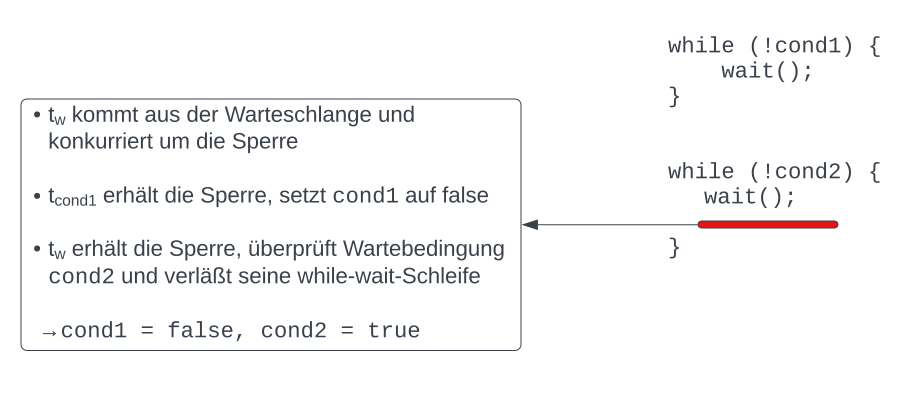
\includegraphics[scale=0.4]{chapters/Anhang/Klausuren/img/cond1cond2}
    \caption{in den rot markierten Bereich konkurriert $t_w$ um die Sperre des Objektes - wenn durch einen anderen Thread, der vor $t_w$ die Sperre erhält, \textit{cond1} auf \textit{false} gesetzt wird, stimmt die Ausgabe nicht mit der erwarteten überein. (Quelle: eigene)}
    \label{fig:cond1cond2}
\end{figure}

\noindent
Die korrekte Wartebedingung sollte lauten:

\begin{minted}[mathescape,
    linenos,
    numbersep=5pt,
    gobble=2,
    fontsize=\small,
    frame=lines,
    framesep=2mm]{java}
    public synchronized void cond1AndCond2() {
        while(!cond1 || !cond2) {
            try {
                wait();
            } catch(InterruptedException e) { }
        }
        System.out.println("cond1 and cond2:" + cond1 + " " + cond2);
    }
\end{minted}\\

Darüber hinaus müßte \code{notifyAll()} nur aufgerufen werden, wenn sowohl \code{cond1} als auch \code{cond2} auf \code{true} gesetzt sind, was leicht in den entsprechenden Methoden überprüft werden kann.
    \chapter{SS19}\label{ch:klausurss19}

\section{Aufgabe 1}

Bei der Aufgabe ist es wichtig, die Anforderungen genau zu beachten.\\
Ob eine Thread die while-wait-Schleife verlassen darf, wird von der Methode \code{tick()} gesteuert - wieviele Ticks ein Thread in der Schleife bleiben soll, wird von dem jeweiligen Thread definiert.\\
Die \code{tick()}-Methode wird von anderen Threads aufgerufen, es kann also durchaus vorkommen, dass mehrmals hintereinander
die \code{notifyAll()}-Methode aufgerufen wird - diese entfernt alle Threads aus der Warteschlange, damit die Threads ihre
Wartebedingungen erneut überprüfen können.\\
da \code{tick()} aber auch gleichzeitig einen Zähler realisieren soll, \textit{muss} es in der Methode auch eine Zählvariable geben, anhand derer die in der while-wait-Schleife enthaltenen Threads feststellen können, wie oft \code{tick()} aufgerufen wurde, um entsprechend aus der Schleife und nachfolgend der Methode herauszukommen.

\begin{figure}
    \centering
    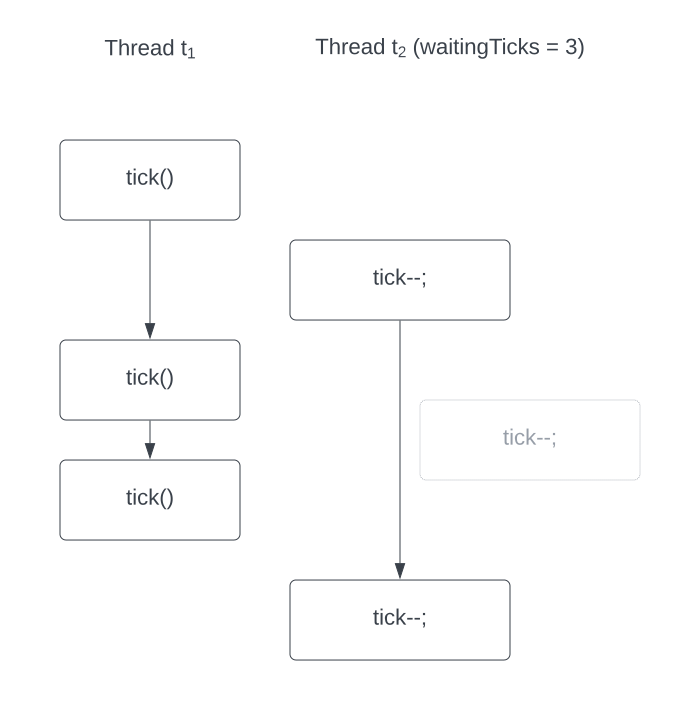
\includegraphics[scale=0.5]{chapters/Anhang/Klausuren/img/tick}
    \caption{Thread $t_1$ ruft 3 mal \texit{tick()} auf. Den Anforderungen nach müsste Thread $t_2$ danach aus der while-wait-Schleife herauskommen, erhält aber nicht die Sperre auf das Objekt von LogicalTime, um seinen eigenen Zähler rechtzeitig zu erniedrigen, bevor $t_1$ erneut \textit{tick()} aufruft. (Quelle: eigene)}
    \label{fig:tick}
\end{figure}

\section{Aufgabe 6}
Auch hier gilt, dass die Aufgabenstellung aufmerksam zu lesen ist.\\
Der Kreis soll erst ausgefüllt werden, wenn die Maustaste gelöst wird.

\begin{minted}[mathescape,
    linenos,
    numbersep=5pt,
    gobble=2,
    frame=lines,
    framesep=2mm]{java}
    private void mousePressed(double x, double y) {
        c = new Circle();
        c.setCenterX(x);
        c.setCenterY(y);
        c.setStroke(Color.RED);
        c.setFill(null); // oder Color.TRANSPARENT
        c.setRadius(RADIUS);
        graphicsPane.getChildren().add(c);
    }

    private void mouseReleased() {
        c.setFill(Color.RED);
        c = null;
    }
\end{minted}

\section{Aufgabe 8}

In der Abbildung \ref{fig:batchmodus} ist links der sequentielle Modus dargestellt, bei dem nach dem Senden einer Nachricht auf die Antwort des Servers gewartet wird, bevor eine neue Nachricht geschickt wird.
Dies wird i.d.R. verwendet, wenn das Senden einer neuen Nachricht abhängig ist von einem Ergebnis, die über die Server-Antwort übermittelt wird, oder wenn mit dem Server interagiert wird (Request abhängig vom Response).\\
Der Batch-Modus auf der rechten Seite der gleichen Abbildung ist schneller, da zwischen dem Senden von Nachrichten nicht auf Antworten gewartet werden müssen. \\
Erst nach dem Senden eine Batches von Nachrichten werden die dem Client zur Verfügung stehenden Antworten ausgelesen.\\

\noindent
In dieser Form des Batch-Modus besteht allerdings die Gefahr, dass es zu Verklemmungen kommt:
\begin{itemize}
    \item Bei dem Client kommen viele Nachrichten an, während er noch sendet.
    \item Die ankommenden Nachrichten für den Client werden gepuffert, bis sie ausgelesen werden (TCP- / OS-seitig).
    \item Läuft der Puffer voll, sorgt die Flusskontrolle (TCP) dafür, dass dem Sender mitgeteilt wird, dass keine Nachrichten mehr empfangen werden können, der Server sendet nicht mehr.
    \item Die zu sendenden Nachrichten des Servers werden in einen Puffer geschrieben.
    \item Der Sende-Puffer des Senders läuft voll.
    \item Bei dem nächsten Sende-Aufruf blockiert der Server, empfangene Nachrichten landen im Empfangspuffer
    \item Der Empfangspuffer des Servers läuft voll, der Client buffert die zu sendenden Nachrichten.
    \item Beide Anwendungen blockieren.
\end{itemize}

\\noindent
Um dieses Problem beim Batch-Modus zu umgehen, werden für das Senden und Empfangen zwei Threads auf Client-Seite erstellt: Ein Thread sendet, ein Thread empfängt. \\
Dadurch kann von dem Client immer wieder sein Empfangspuffer geleert werden, der Server wird beim Senden nicht blockiert.

\begin{figure}
    \centering
    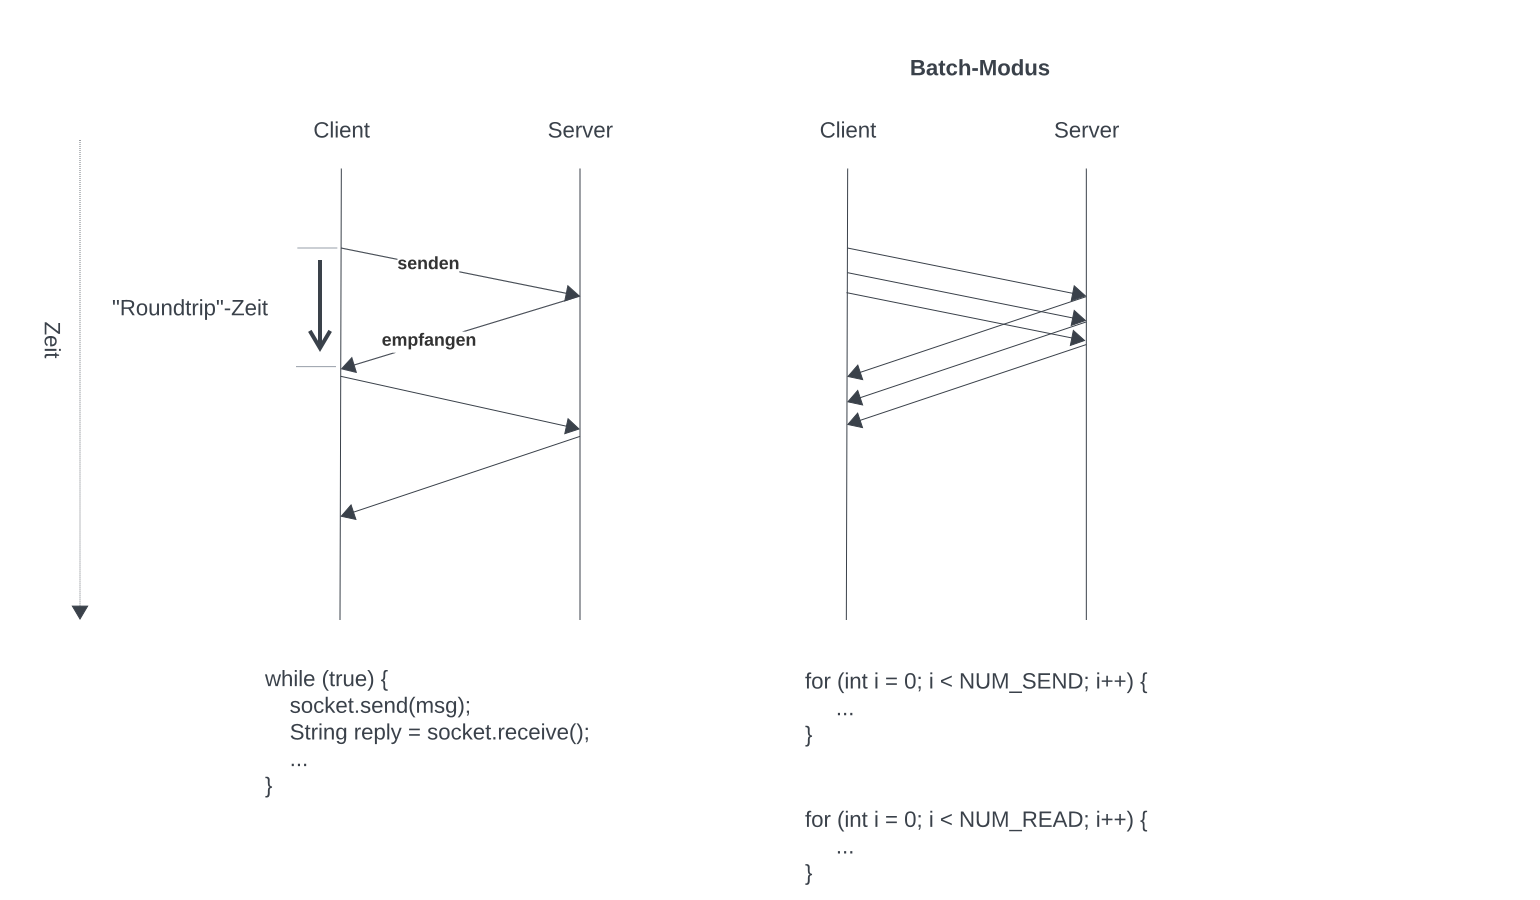
\includegraphics[scale=0.4]{chapters/Anhang/Klausuren/img/batchmodus}
    \caption{Vereinfachte Darstellung sequentieller Kommunikation und Batch-Modus (Quelle: eigene)}
    \label{fig:batchmodus}
\end{figure}
    
\begin{appendices}
    
\begin{appendices}
    \input{chapters/Anhang/Zusatzaufgaben/index}
    \input{chapters/Anhang/Klausuren/ws13}
    \input{chapters/Anhang/Klausuren/ws15-16}
    \input{chapters/Anhang/Klausuren/ws16-17}
    \input{chapters/Anhang/Klausuren/ss19}
    \input{chapters/Anhang/Präsenzphase/index}

\end{appendices}

    \chapter{WS13}\label{ch:klausurws13}

\section{Aufgabe 1}
\subsection{Lösungsvorschlag}


\begin{minted}[mathescape,
    linenos,
    numbersep=5pt,
    gobble=2,
    fontsize=\small,
    frame=lines,
    framesep=2mm]{java}
    class Zahlenschloss {

        private int[] kombination;

        private int[] state;

        private boolean opened = false;

        public Zahlenschloss(int[] kombination) {
            this.kombination = kombination;
            this.state = new int[kombination.length];
        }

        public int anzahlRaedchen() {
            return kombination.length;
        }

        public synchronized int lesen(int radnummer) {
            return state[radnummer];
        }

        public synchronized void drehen(int radnummer, int zahl) {

            state[radnummer] = zahl;
            opened = true;
            for (int i = 0; i < anzahlRaedchen(); i++) {
                if (lesen(i) != kombination[i]) {
                    opened = false;
                    break;
                }
            }

            if (opened) {
                this.notify();
            }
        }

        public synchronized void warten() {

            while (!opened) {
                try {
                    this.wait();
                } catch (InterruptedException ignored) {}
            }
        }
    }
\end{minted}\\


\subsection{Anmerkung und Ergänzungen}

\begin{itemize}
    \item Es wird eine Wartebedingung benötigt, und zwar für die Methode \code{warten()}; ankommende Threads werden
    in die Warteschlange des Zahlenschloss-Objektes geschickt, wenn \code{opened} auf false gesetzt ist, ansonsten
    verlassen diese direkt die Methode wieder.\\
    Die Methode \code{drehen} benötigt keine separate Wartebedingung.
    Es reicht aus, sicherzustellen, dass das Zahlenschloss nicht gleichzeitig von anderen Threads benutzt werden kann:
    Die Methode \code{drehen} ist hierfür synchronisiert, damit das Zahlenschloss {insg.} immer nur eine Zustandsänderung
    erfährt - es sind andere Implementierungen möglich, in denen das Zahlenschloss dann von mehreren Threads gleichzeitig
    genutzt werden darf, wenn sich die Zugriffe anhand der ``Ziel``-\code{radnummer} unterscheiden, {bspw.} durch Mutex-Semaphore,
    die pro Radnummer verwendet werden\footnote{
        der gleichzeitige Zugriff auf unterschiedliche Arrays-Indizes ist erlaubt, s. `´17.4.1. Shared Variables``: \url{https://docs.oracle.com/javase/specs/jls/se21/html/jls-17.html#jls-1.4.1} - abgerufen 14.2.2024
    }.
    \item Es gibt nur eine Wartebedingung, von daher sollte \code{notify()} genügen.\\
    Wenn wir allerdings davon ausgehen, dass mehrere Threads über die Methode \code{warten()} in die Warteschlange des Objektes eingereiht worden sind,  sollte \code{notifyAll()} verwendet werden (siehe hierzu auch Abschnitt \ref{subsec:notifyAll}).
    Dennoch ist nicht garantiert, dass auch alle Threads aus der Warteschlange gelangen, denn es kann sein, dass ein anderer Thread die Methode \code{drehen()} betritt, dort die
    Zahlenkombination ändert und \code{opened} wieder auf \code{false} gesetzt wird. \\
    Ein anderer Thread, der nun in  \code{warten()} an die Reihe kommt, überprüft die Wartebedingung, und wird wieder in die Warteschlange eingereiht.
    Es ist also durchaus möglich, dass ein Thread nicht mehr aus der Methode \code{warten()} herauskommt.\\
    Dies könnte bspw. dadurch verhindert werden, dass die Threads in eine Queue gepackt werden, und in \code{drehen()} eine Wartebedingung eingefügt wird, die erst erfüllt ist,
    wenn die Queue geleert wurde oder aus ihr entnommen wurde, in der Reihenfolge, in der die Threads in die Queue eingereiht worden sind (\textit{FIFO}) (s. a. Abschnitt~\ref{subsec:readerwriterproblem}).
    \item Bei der Teilaufgabe mit der Schleife muss die komplette Schleife synchronisiert werden, was man durch ein \code{synchronized}-Statement erreicht\footnote{siehe Abschnitt~\ref{subsec:synchronizedstatement}.}
    \begin{minted}[mathescape,
        linenos,
        numbersep=5pt,
        gobble=2,
        fontsize=\small,
        frame=lines,
        framesep=2mm]{java}
        synchronized (zk) {
            for (int i = 0; i < anzahlRaedchen; i++) {
                System.out.println(zk.lesen(i));
            }
        }
    \end{minted}
    Ansonsten läuft man Gefahr, dass sich nach Auslesen der 1. Position der Wert von Position 2 geändert hat und dadurch eine
    Zahlenkombination ausgegeben wird, die es nicht gegeben hat:
    \begin{enumerate}
        \item $K\coloneqq[0, 0, 0]$
        \item Position $K_0$ wird ausgelesen und liefert $0$.
        \item Thread ändert $K_0$ zu $1$ $\implies K\coloneqq[1, 0, 0] $.
        \item Thread ändert $K_1$ zu $2$ $\implies K\coloneqq[1, 2, 0] $.
        \item Thread ändert $K_2$ zu $3$ $\implies K\coloneqq[1, 2, 3] $.
        \item Positionen $K_1$ und $K_2$ werden ausgelesen und liefern: $2, 3$
        \item Ausgabe: $0, 2, 3$ - diese Kombination hat es in dem Fall aber tatsächlich nicht gegeben.
    \end{enumerate}
\end{itemize}

\begin{tcolorbox}[colback=red!20,color=white,title=Anmerkung]
    Die Methode \code{lesen()} als \code{synchronized} zu markieren könnte man sich vlt. sparen, wenn man davon ausgeht,
    dass die Methode ohnehin in einem \code{synchronized}-Statement verwendet wird, um alle Rädchen abzulesen.\\
    Mehrere Threads können also nicht parallel auf unterschiedliche Positionen des Feldes zugreifen, wenn die Methode
    synchronisiert ist.\\
    Allerdings ist sowohl das Skript als auch das Buch recht klar, was in dieser Situation geschehen muss (s. Skript Fopt1/2, S. 9, außerdem \cite[31, Abschnitt 2.3.6]{Oec22}): Es muss (in diesem Kurs) immer \code{synchronized} verwendet werden, wenn gleichzeitig
    Daten geschrieben und gleichzeitig diese Daten gelesen werden sollen - und eine andere Implementierung, bei der die
    einzelnen Positionen ``gelocked`` sind, so dass ein gleichzeitiger Zugriff auf unterschiedliche Rädchen möglich ist, war nicht gefordert.\\
    Ggfl. würde in anderen Implementierungen der Einsatz von \code{AtomicReferenceArray}\footnote{s. \cite[157 ff.]{Oec22}
    s. ``Class AtomicReferenceArray<E>``: \url{https://docs.oracle.com/en/java/javase/21/docs/api/java.base/java/util/concurrent/atomic/AtomicReferenceArray.html} - abgerufen 15.2.2024
    } Sinn machen, aber das Lehrmaterial ist bereits sehr eindeutig bzgl. der Verwendung von \code{synchronized}.
\end{tcolorbox}



\section{Aufgabe 3}
\subsection{Lösungsvorschlag}

\subsection*{Statische Parallelität}
Statische Parallelität erlaubt es einem Server, eine \textit{fixe} Anzahl von Verbindungen gleichzeitig zu bedienen.\\
Hierbei wird ein Feld von Threads erstellt, wobei jeder Thread das \code{ServerSocket}-Objekt als Referenz übergeben bekommt.
In der \code{run()}-Methode wird dann über \code{accept()} in einer Endlosschleife auf eingehende Verbindungen gewartet, die dann so lange bedient werden, bis sich ein Client wieder abmeldet (oder eine andere Abbruchbedingung erfüllt ist, wie z.B. ein \code{SocketTimeout}).\\
Das sich ein Client abmeldet, bekommt man bspw. dadurch mit, dass \code{null} beim Lesen von einer Nachricht des Clients zurückgegeben wird (vgl. \cite[286]{Oec22}. \\
Siehe Abschnitt~\ref{sec:seqparserver} für ein Implementierungsbeispiel.



\subsection*{Dynamische Parallelität}

Bei der \textbf{Dynamischer Parallelität} erzeugt der Server für jede Verbindung einen neuen Thread, der so lange läuft, bis der Client die Verbindung wieder trennt.\\
Die Anzahl der Threads ändert sich dadurch laufend.\\
Wird die max. Anzahl erlaubter Threads nicht kontrolliert, kann es zu einer Überlastung des Server-Rechners kommen (bspw. durch einen Denial-of-Service-Angriff.)\\

\noindent
I.d.R. ist eine Mischform aus beidem geeignet, um mehrere Clients gleichzeitig bedienen zu können, und dabei nicht Gefahr zu laufen, durch dynamisches, unbegrenztes Wachstum der Anzahl der Threads überlastet zu werden.

    \chapter{WS13}\label{ch:klausurws5-16}

\section{Rechteck-Scroll (SS15 Aufgabe 2)}

Aufgabenstellung unklar.\\
Mögliche Implementierung unter \url{https://github.com/ThorstenSuckow/fopt/tree/main/src/main/java/klausurvorbereitung/foptws1516/MouseDragsSquareDemo}.

\section{Rechteck-Scroll (WS15/16 Aufgabe 1)}

Aufgabenstellung unklar.\\
Mögliche Implementierung unter \url{https://github.com/ThorstenSuckow/fopt/tree/main/src/main/java/klausurvorbereitung/foptws1516/MaxWeightDemo}.\\

\noindent
Es gibt nur eine Warteschlange für Threads in \code{use()}, es gibt keine Wartebedingung in \code{dontUse()} und damit auch keine weitere Warteschlange.\\
Es sind durch die Zugriffe auf unterschiedliche Indizes allerdings mehrere Wartebedingungen vorhanden, weshalb hab \code{notifyAll()} nutzen sollte,
sobald ein Zugriff auf ein Feld nach Aufruf von \code{dontUse} wieder möglich wird.\\
Ansonsten bestünde die Gefahr, dass bei dem Einsatz von \code{notify()} ein wartender Thread nicht geweckt wird, obwohl er weiterlaufen könnte:\\
Angenommen, das Feld $F$ hat eine Länge von $3$, das \code{maxWeight} ist mit $2$ konfiguriert.
Thread $t_1$ mit einer Laufzeit von $200\ sek$ bekommt Zugriff auf $F_0$, setzt $currentWeight$ auf $1$.\\
Thread $t_2$ mit einer Laufzeit von $1\ sek$ möchte auf $F_1$ zugreifen, setzt $currentWeight=2$ in die Warteschlange.\\
Thread $t_3$ meldet Zugriff auf $F_0$ an und gelangt in die Warteschlange.\\
Thread $t_4$ meldet Zugriff auf $F_1$ an und gelangt in die Warteschlange.\\
Thread $t_2$ ist mit der Bearbeitung von $F_1$ fertig, $currentWeight$ wird auf $1$ gesetzt, \code{notify()} wird aufgerufen.\\
Thread $t_3$ wird aus der Warteschlange geholt, kann aber nicht weiterarbeiten, da $F_0$ noch durch den länger dauernden $t_1$ blockiert ist, und kommt wieder in die Warteschlange.\\

\noindent
Offensichtlich hätte in dem Beispiel \code{notifyAll()} dazu geführt, dass auch $T_4$ seine Wartebedingung hätte überprüfen können, und hätte so Zugriff auf $F_1$ bekommen.
Stattdessen muss nun gewartet werden, bis das nächste \code{notify()} aufgerufen wird, oder ein neu ankommender Thread $F_1$ belegt.

    \chapter{WS16-17}\label{ch:klausurws16-17}

\section{Aufgabe 1}
\subsection{Lösungshinweis}

Die erste Aufgabe verdeutlicht, was bei einem \code{notifyAll()} und unsauber gesetzten Wartebedingungen passieren kann.\\
Sei folgender Quellcode gegeben:


\begin{minted}[mathescape,
    linenos,
    numbersep=5pt,
    gobble=2,
    fontsize=\small,
    frame=lines,
    framesep=2mm]{java}
    class Cond1AndCond2 {

        private boolean cond1;
        private boolean cond2;

        public synchronized void setCond1(boolean c) {
            cond1 = c;
            notifyAll();
        }

        public synchronized void setCond2(boolean c) {
            cond2 = c;
            notifyAll();
        }

        public synchronized void cond1AndCond2() {
            while(!cond1) {
                try {
                    wait();
                } catch(InterruptedException e) { }
            }

            while(!cond2) {
                try {
                    wait();
                } catch(InterruptedException e) {}
            }
            System.out.println("cond1 and cond2:" + cond1 + " " + cond2);
        }
    }
\end{minted}\\

Man sollte auf den ersten Blick meinen, dass \code{cond1} und \code{cond2} beide \code{true} sein müssen, damit die Ausgabe erfolgt.\\
Tatsächlich ist es aber so, dass es in der Methode zwei unterschiedliche Wartebedingungen gibt.\\
Die erste Wartebedingung schickt einen Thread in die Warteschlange, wenn \code{cond1 == false} gilt.\\
Setzt ein anderer Thread über \code{setCond1(true)} das Attribut entsprechend auf \code{true}, bewirkt der nachfolgende Aufruf von \code{notifyAll()}, dass alle \textit{wartenden} Threads aus der Warteschlange entfernt werden und erneut um eine Sperre des Objektes konkurrieren.\\
Erhält ein entsprechender Thread $t_w$ die Sperre auf das Objekt und kann seine \textit{while-wait-Schleife} verlassen, kann es vorkommen, dass er erneut in die Warteschlange eingereiht wird, wegen der nachfolgenden Wartebedingung \code{cond2 == false}.\\
Angenommen, ein weiterer Thread ruft nun \code{setCond2(true)} auf, und $t_w$ kommt aus der Warteschlange und konkurriert erneut und um die Sperre des Objektes, dann kann es vorkommen, das ein anderer Thread zunächst die Sperre erhält, \code{cond1} wieder auf \code{false} setzt, dann erhält $t_w$ die Sperre, überprüft die Wartebedingung \code{cond2 == false}.\\
Wegen \code{cond2} gelangt er aus der \textit{while-wait-Schleife} und die Ausgabe erfolgt - da zwischenzeitlich \code{cond1} wieder auf \code{false} gesetzt wurde, ist die erwartete Ausgabe nicht \code{true true}, sondern \code{false true} (s. Abbildung \ref{fig:cond1cond2}).\\

\begin{figure}
    \centering
    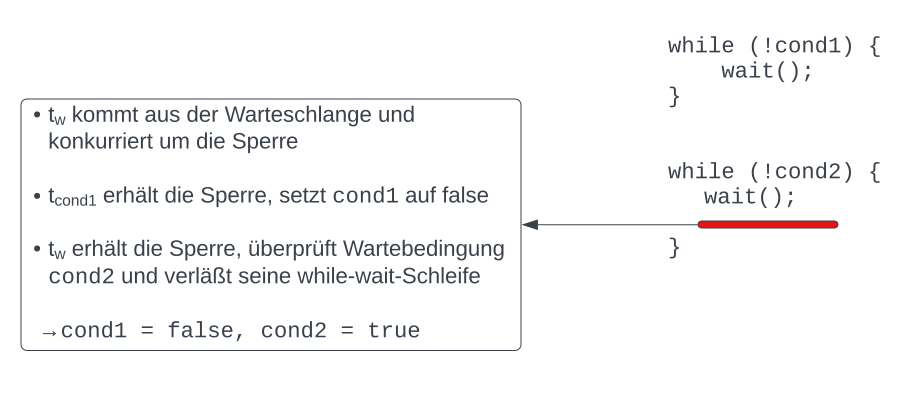
\includegraphics[scale=0.4]{chapters/Anhang/Klausuren/img/cond1cond2}
    \caption{in den rot markierten Bereich konkurriert $t_w$ um die Sperre des Objektes - wenn durch einen anderen Thread, der vor $t_w$ die Sperre erhält, \textit{cond1} auf \textit{false} gesetzt wird, stimmt die Ausgabe nicht mit der erwarteten überein. (Quelle: eigene)}
    \label{fig:cond1cond2}
\end{figure}

\noindent
Die korrekte Wartebedingung sollte lauten:

\begin{minted}[mathescape,
    linenos,
    numbersep=5pt,
    gobble=2,
    fontsize=\small,
    frame=lines,
    framesep=2mm]{java}
    public synchronized void cond1AndCond2() {
        while(!cond1 || !cond2) {
            try {
                wait();
            } catch(InterruptedException e) { }
        }
        System.out.println("cond1 and cond2:" + cond1 + " " + cond2);
    }
\end{minted}\\

Darüber hinaus müßte \code{notifyAll()} nur aufgerufen werden, wenn sowohl \code{cond1} als auch \code{cond2} auf \code{true} gesetzt sind, was leicht in den entsprechenden Methoden überprüft werden kann.
    \chapter{SS19}\label{ch:klausurss19}

\section{Aufgabe 1}

Bei der Aufgabe ist es wichtig, die Anforderungen genau zu beachten.\\
Ob eine Thread die while-wait-Schleife verlassen darf, wird von der Methode \code{tick()} gesteuert - wieviele Ticks ein Thread in der Schleife bleiben soll, wird von dem jeweiligen Thread definiert.\\
Die \code{tick()}-Methode wird von anderen Threads aufgerufen, es kann also durchaus vorkommen, dass mehrmals hintereinander
die \code{notifyAll()}-Methode aufgerufen wird - diese entfernt alle Threads aus der Warteschlange, damit die Threads ihre
Wartebedingungen erneut überprüfen können.\\
da \code{tick()} aber auch gleichzeitig einen Zähler realisieren soll, \textit{muss} es in der Methode auch eine Zählvariable geben, anhand derer die in der while-wait-Schleife enthaltenen Threads feststellen können, wie oft \code{tick()} aufgerufen wurde, um entsprechend aus der Schleife und nachfolgend der Methode herauszukommen.

\begin{figure}
    \centering
    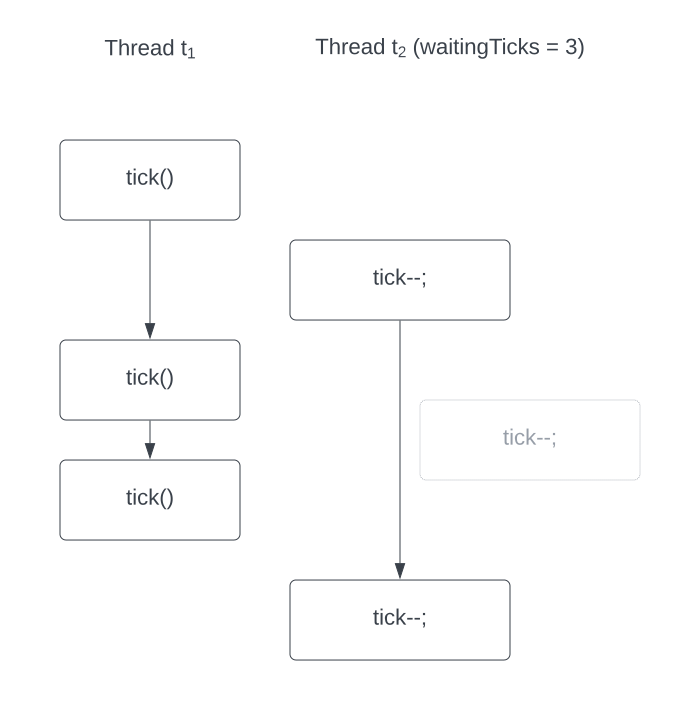
\includegraphics[scale=0.5]{chapters/Anhang/Klausuren/img/tick}
    \caption{Thread $t_1$ ruft 3 mal \texit{tick()} auf. Den Anforderungen nach müsste Thread $t_2$ danach aus der while-wait-Schleife herauskommen, erhält aber nicht die Sperre auf das Objekt von LogicalTime, um seinen eigenen Zähler rechtzeitig zu erniedrigen, bevor $t_1$ erneut \textit{tick()} aufruft. (Quelle: eigene)}
    \label{fig:tick}
\end{figure}

\section{Aufgabe 6}
Auch hier gilt, dass die Aufgabenstellung aufmerksam zu lesen ist.\\
Der Kreis soll erst ausgefüllt werden, wenn die Maustaste gelöst wird.

\begin{minted}[mathescape,
    linenos,
    numbersep=5pt,
    gobble=2,
    frame=lines,
    framesep=2mm]{java}
    private void mousePressed(double x, double y) {
        c = new Circle();
        c.setCenterX(x);
        c.setCenterY(y);
        c.setStroke(Color.RED);
        c.setFill(null); // oder Color.TRANSPARENT
        c.setRadius(RADIUS);
        graphicsPane.getChildren().add(c);
    }

    private void mouseReleased() {
        c.setFill(Color.RED);
        c = null;
    }
\end{minted}

\section{Aufgabe 8}

In der Abbildung \ref{fig:batchmodus} ist links der sequentielle Modus dargestellt, bei dem nach dem Senden einer Nachricht auf die Antwort des Servers gewartet wird, bevor eine neue Nachricht geschickt wird.
Dies wird i.d.R. verwendet, wenn das Senden einer neuen Nachricht abhängig ist von einem Ergebnis, die über die Server-Antwort übermittelt wird, oder wenn mit dem Server interagiert wird (Request abhängig vom Response).\\
Der Batch-Modus auf der rechten Seite der gleichen Abbildung ist schneller, da zwischen dem Senden von Nachrichten nicht auf Antworten gewartet werden müssen. \\
Erst nach dem Senden eine Batches von Nachrichten werden die dem Client zur Verfügung stehenden Antworten ausgelesen.\\

\noindent
In dieser Form des Batch-Modus besteht allerdings die Gefahr, dass es zu Verklemmungen kommt:
\begin{itemize}
    \item Bei dem Client kommen viele Nachrichten an, während er noch sendet.
    \item Die ankommenden Nachrichten für den Client werden gepuffert, bis sie ausgelesen werden (TCP- / OS-seitig).
    \item Läuft der Puffer voll, sorgt die Flusskontrolle (TCP) dafür, dass dem Sender mitgeteilt wird, dass keine Nachrichten mehr empfangen werden können, der Server sendet nicht mehr.
    \item Die zu sendenden Nachrichten des Servers werden in einen Puffer geschrieben.
    \item Der Sende-Puffer des Senders läuft voll.
    \item Bei dem nächsten Sende-Aufruf blockiert der Server, empfangene Nachrichten landen im Empfangspuffer
    \item Der Empfangspuffer des Servers läuft voll, der Client buffert die zu sendenden Nachrichten.
    \item Beide Anwendungen blockieren.
\end{itemize}

\\noindent
Um dieses Problem beim Batch-Modus zu umgehen, werden für das Senden und Empfangen zwei Threads auf Client-Seite erstellt: Ein Thread sendet, ein Thread empfängt. \\
Dadurch kann von dem Client immer wieder sein Empfangspuffer geleert werden, der Server wird beim Senden nicht blockiert.

\begin{figure}
    \centering
    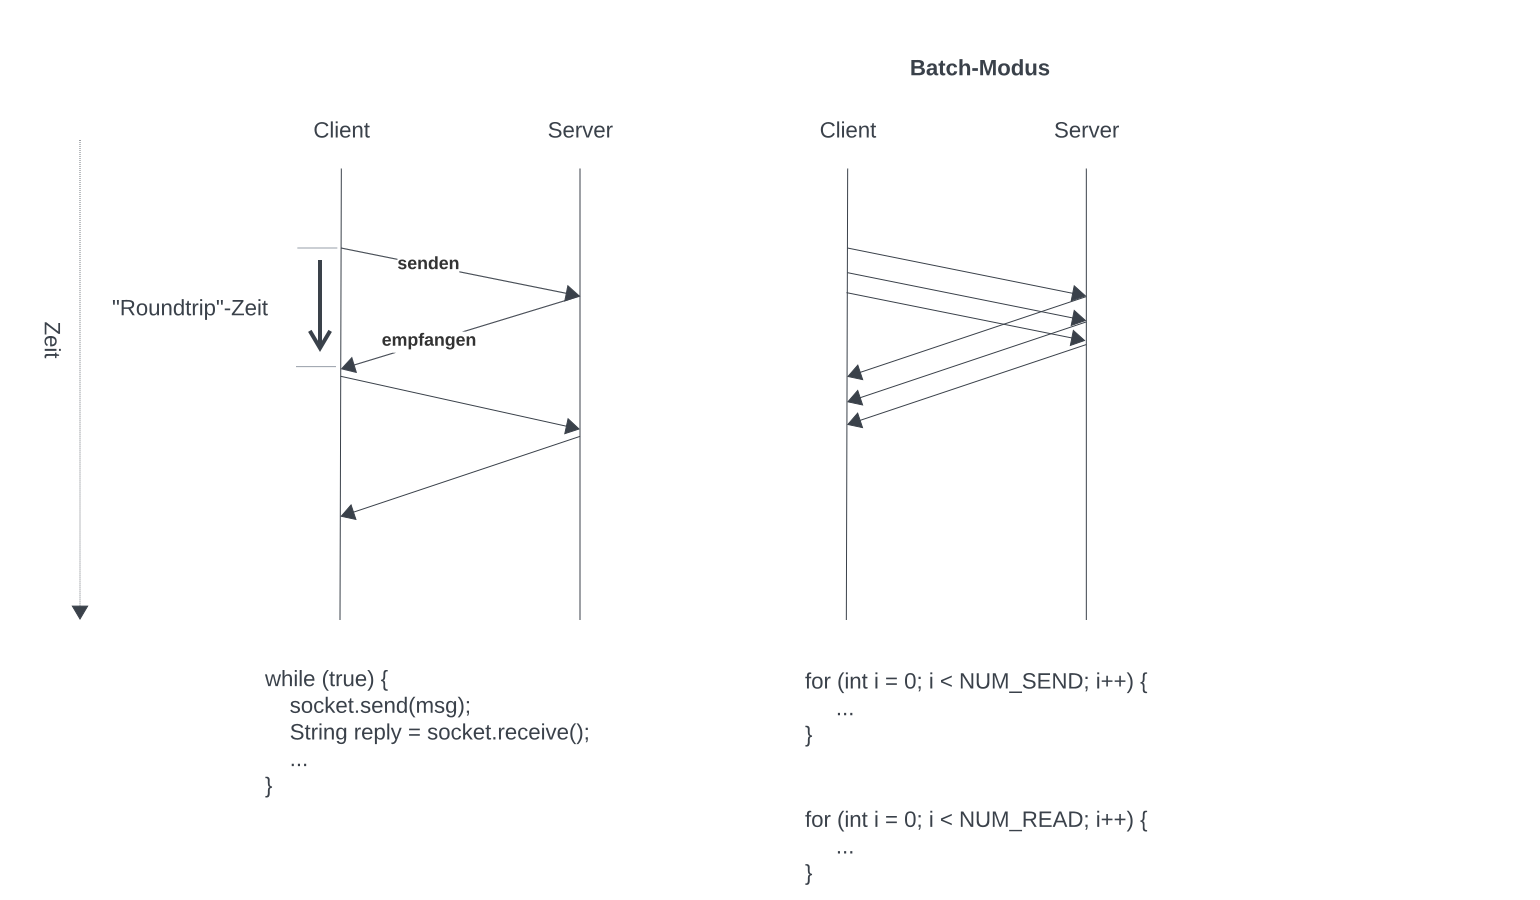
\includegraphics[scale=0.4]{chapters/Anhang/Klausuren/img/batchmodus}
    \caption{Vereinfachte Darstellung sequentieller Kommunikation und Batch-Modus (Quelle: eigene)}
    \label{fig:batchmodus}
\end{figure}
    
\begin{appendices}
    \input{chapters/Anhang/Zusatzaufgaben/index}
    \input{chapters/Anhang/Klausuren/ws13}
    \input{chapters/Anhang/Klausuren/ws15-16}
    \input{chapters/Anhang/Klausuren/ws16-17}
    \input{chapters/Anhang/Klausuren/ss19}
    \input{chapters/Anhang/Präsenzphase/index}

\end{appendices}


\end{appendices}


\end{appendices}



\begin{appendices}
    
\begin{appendices}
    
\begin{appendices}
    \input{chapters/Anhang/Zusatzaufgaben/index}
    \input{chapters/Anhang/Klausuren/ws13}
    \input{chapters/Anhang/Klausuren/ws15-16}
    \input{chapters/Anhang/Klausuren/ws16-17}
    \input{chapters/Anhang/Klausuren/ss19}
    \input{chapters/Anhang/Präsenzphase/index}

\end{appendices}

    \chapter{WS13}\label{ch:klausurws13}

\section{Aufgabe 1}
\subsection{Lösungsvorschlag}


\begin{minted}[mathescape,
    linenos,
    numbersep=5pt,
    gobble=2,
    fontsize=\small,
    frame=lines,
    framesep=2mm]{java}
    class Zahlenschloss {

        private int[] kombination;

        private int[] state;

        private boolean opened = false;

        public Zahlenschloss(int[] kombination) {
            this.kombination = kombination;
            this.state = new int[kombination.length];
        }

        public int anzahlRaedchen() {
            return kombination.length;
        }

        public synchronized int lesen(int radnummer) {
            return state[radnummer];
        }

        public synchronized void drehen(int radnummer, int zahl) {

            state[radnummer] = zahl;
            opened = true;
            for (int i = 0; i < anzahlRaedchen(); i++) {
                if (lesen(i) != kombination[i]) {
                    opened = false;
                    break;
                }
            }

            if (opened) {
                this.notify();
            }
        }

        public synchronized void warten() {

            while (!opened) {
                try {
                    this.wait();
                } catch (InterruptedException ignored) {}
            }
        }
    }
\end{minted}\\


\subsection{Anmerkung und Ergänzungen}

\begin{itemize}
    \item Es wird eine Wartebedingung benötigt, und zwar für die Methode \code{warten()}; ankommende Threads werden
    in die Warteschlange des Zahlenschloss-Objektes geschickt, wenn \code{opened} auf false gesetzt ist, ansonsten
    verlassen diese direkt die Methode wieder.\\
    Die Methode \code{drehen} benötigt keine separate Wartebedingung.
    Es reicht aus, sicherzustellen, dass das Zahlenschloss nicht gleichzeitig von anderen Threads benutzt werden kann:
    Die Methode \code{drehen} ist hierfür synchronisiert, damit das Zahlenschloss {insg.} immer nur eine Zustandsänderung
    erfährt - es sind andere Implementierungen möglich, in denen das Zahlenschloss dann von mehreren Threads gleichzeitig
    genutzt werden darf, wenn sich die Zugriffe anhand der ``Ziel``-\code{radnummer} unterscheiden, {bspw.} durch Mutex-Semaphore,
    die pro Radnummer verwendet werden\footnote{
        der gleichzeitige Zugriff auf unterschiedliche Arrays-Indizes ist erlaubt, s. `´17.4.1. Shared Variables``: \url{https://docs.oracle.com/javase/specs/jls/se21/html/jls-17.html#jls-1.4.1} - abgerufen 14.2.2024
    }.
    \item Es gibt nur eine Wartebedingung, von daher sollte \code{notify()} genügen.\\
    Wenn wir allerdings davon ausgehen, dass mehrere Threads über die Methode \code{warten()} in die Warteschlange des Objektes eingereiht worden sind,  sollte \code{notifyAll()} verwendet werden (siehe hierzu auch Abschnitt \ref{subsec:notifyAll}).
    Dennoch ist nicht garantiert, dass auch alle Threads aus der Warteschlange gelangen, denn es kann sein, dass ein anderer Thread die Methode \code{drehen()} betritt, dort die
    Zahlenkombination ändert und \code{opened} wieder auf \code{false} gesetzt wird. \\
    Ein anderer Thread, der nun in  \code{warten()} an die Reihe kommt, überprüft die Wartebedingung, und wird wieder in die Warteschlange eingereiht.
    Es ist also durchaus möglich, dass ein Thread nicht mehr aus der Methode \code{warten()} herauskommt.\\
    Dies könnte bspw. dadurch verhindert werden, dass die Threads in eine Queue gepackt werden, und in \code{drehen()} eine Wartebedingung eingefügt wird, die erst erfüllt ist,
    wenn die Queue geleert wurde oder aus ihr entnommen wurde, in der Reihenfolge, in der die Threads in die Queue eingereiht worden sind (\textit{FIFO}) (s. a. Abschnitt~\ref{subsec:readerwriterproblem}).
    \item Bei der Teilaufgabe mit der Schleife muss die komplette Schleife synchronisiert werden, was man durch ein \code{synchronized}-Statement erreicht\footnote{siehe Abschnitt~\ref{subsec:synchronizedstatement}.}
    \begin{minted}[mathescape,
        linenos,
        numbersep=5pt,
        gobble=2,
        fontsize=\small,
        frame=lines,
        framesep=2mm]{java}
        synchronized (zk) {
            for (int i = 0; i < anzahlRaedchen; i++) {
                System.out.println(zk.lesen(i));
            }
        }
    \end{minted}
    Ansonsten läuft man Gefahr, dass sich nach Auslesen der 1. Position der Wert von Position 2 geändert hat und dadurch eine
    Zahlenkombination ausgegeben wird, die es nicht gegeben hat:
    \begin{enumerate}
        \item $K\coloneqq[0, 0, 0]$
        \item Position $K_0$ wird ausgelesen und liefert $0$.
        \item Thread ändert $K_0$ zu $1$ $\implies K\coloneqq[1, 0, 0] $.
        \item Thread ändert $K_1$ zu $2$ $\implies K\coloneqq[1, 2, 0] $.
        \item Thread ändert $K_2$ zu $3$ $\implies K\coloneqq[1, 2, 3] $.
        \item Positionen $K_1$ und $K_2$ werden ausgelesen und liefern: $2, 3$
        \item Ausgabe: $0, 2, 3$ - diese Kombination hat es in dem Fall aber tatsächlich nicht gegeben.
    \end{enumerate}
\end{itemize}

\begin{tcolorbox}[colback=red!20,color=white,title=Anmerkung]
    Die Methode \code{lesen()} als \code{synchronized} zu markieren könnte man sich vlt. sparen, wenn man davon ausgeht,
    dass die Methode ohnehin in einem \code{synchronized}-Statement verwendet wird, um alle Rädchen abzulesen.\\
    Mehrere Threads können also nicht parallel auf unterschiedliche Positionen des Feldes zugreifen, wenn die Methode
    synchronisiert ist.\\
    Allerdings ist sowohl das Skript als auch das Buch recht klar, was in dieser Situation geschehen muss (s. Skript Fopt1/2, S. 9, außerdem \cite[31, Abschnitt 2.3.6]{Oec22}): Es muss (in diesem Kurs) immer \code{synchronized} verwendet werden, wenn gleichzeitig
    Daten geschrieben und gleichzeitig diese Daten gelesen werden sollen - und eine andere Implementierung, bei der die
    einzelnen Positionen ``gelocked`` sind, so dass ein gleichzeitiger Zugriff auf unterschiedliche Rädchen möglich ist, war nicht gefordert.\\
    Ggfl. würde in anderen Implementierungen der Einsatz von \code{AtomicReferenceArray}\footnote{s. \cite[157 ff.]{Oec22}
    s. ``Class AtomicReferenceArray<E>``: \url{https://docs.oracle.com/en/java/javase/21/docs/api/java.base/java/util/concurrent/atomic/AtomicReferenceArray.html} - abgerufen 15.2.2024
    } Sinn machen, aber das Lehrmaterial ist bereits sehr eindeutig bzgl. der Verwendung von \code{synchronized}.
\end{tcolorbox}



\section{Aufgabe 3}
\subsection{Lösungsvorschlag}

\subsection*{Statische Parallelität}
Statische Parallelität erlaubt es einem Server, eine \textit{fixe} Anzahl von Verbindungen gleichzeitig zu bedienen.\\
Hierbei wird ein Feld von Threads erstellt, wobei jeder Thread das \code{ServerSocket}-Objekt als Referenz übergeben bekommt.
In der \code{run()}-Methode wird dann über \code{accept()} in einer Endlosschleife auf eingehende Verbindungen gewartet, die dann so lange bedient werden, bis sich ein Client wieder abmeldet (oder eine andere Abbruchbedingung erfüllt ist, wie z.B. ein \code{SocketTimeout}).\\
Das sich ein Client abmeldet, bekommt man bspw. dadurch mit, dass \code{null} beim Lesen von einer Nachricht des Clients zurückgegeben wird (vgl. \cite[286]{Oec22}. \\
Siehe Abschnitt~\ref{sec:seqparserver} für ein Implementierungsbeispiel.



\subsection*{Dynamische Parallelität}

Bei der \textbf{Dynamischer Parallelität} erzeugt der Server für jede Verbindung einen neuen Thread, der so lange läuft, bis der Client die Verbindung wieder trennt.\\
Die Anzahl der Threads ändert sich dadurch laufend.\\
Wird die max. Anzahl erlaubter Threads nicht kontrolliert, kann es zu einer Überlastung des Server-Rechners kommen (bspw. durch einen Denial-of-Service-Angriff.)\\

\noindent
I.d.R. ist eine Mischform aus beidem geeignet, um mehrere Clients gleichzeitig bedienen zu können, und dabei nicht Gefahr zu laufen, durch dynamisches, unbegrenztes Wachstum der Anzahl der Threads überlastet zu werden.

    \chapter{WS13}\label{ch:klausurws5-16}

\section{Rechteck-Scroll (SS15 Aufgabe 2)}

Aufgabenstellung unklar.\\
Mögliche Implementierung unter \url{https://github.com/ThorstenSuckow/fopt/tree/main/src/main/java/klausurvorbereitung/foptws1516/MouseDragsSquareDemo}.

\section{Rechteck-Scroll (WS15/16 Aufgabe 1)}

Aufgabenstellung unklar.\\
Mögliche Implementierung unter \url{https://github.com/ThorstenSuckow/fopt/tree/main/src/main/java/klausurvorbereitung/foptws1516/MaxWeightDemo}.\\

\noindent
Es gibt nur eine Warteschlange für Threads in \code{use()}, es gibt keine Wartebedingung in \code{dontUse()} und damit auch keine weitere Warteschlange.\\
Es sind durch die Zugriffe auf unterschiedliche Indizes allerdings mehrere Wartebedingungen vorhanden, weshalb hab \code{notifyAll()} nutzen sollte,
sobald ein Zugriff auf ein Feld nach Aufruf von \code{dontUse} wieder möglich wird.\\
Ansonsten bestünde die Gefahr, dass bei dem Einsatz von \code{notify()} ein wartender Thread nicht geweckt wird, obwohl er weiterlaufen könnte:\\
Angenommen, das Feld $F$ hat eine Länge von $3$, das \code{maxWeight} ist mit $2$ konfiguriert.
Thread $t_1$ mit einer Laufzeit von $200\ sek$ bekommt Zugriff auf $F_0$, setzt $currentWeight$ auf $1$.\\
Thread $t_2$ mit einer Laufzeit von $1\ sek$ möchte auf $F_1$ zugreifen, setzt $currentWeight=2$ in die Warteschlange.\\
Thread $t_3$ meldet Zugriff auf $F_0$ an und gelangt in die Warteschlange.\\
Thread $t_4$ meldet Zugriff auf $F_1$ an und gelangt in die Warteschlange.\\
Thread $t_2$ ist mit der Bearbeitung von $F_1$ fertig, $currentWeight$ wird auf $1$ gesetzt, \code{notify()} wird aufgerufen.\\
Thread $t_3$ wird aus der Warteschlange geholt, kann aber nicht weiterarbeiten, da $F_0$ noch durch den länger dauernden $t_1$ blockiert ist, und kommt wieder in die Warteschlange.\\

\noindent
Offensichtlich hätte in dem Beispiel \code{notifyAll()} dazu geführt, dass auch $T_4$ seine Wartebedingung hätte überprüfen können, und hätte so Zugriff auf $F_1$ bekommen.
Stattdessen muss nun gewartet werden, bis das nächste \code{notify()} aufgerufen wird, oder ein neu ankommender Thread $F_1$ belegt.

    \chapter{WS16-17}\label{ch:klausurws16-17}

\section{Aufgabe 1}
\subsection{Lösungshinweis}

Die erste Aufgabe verdeutlicht, was bei einem \code{notifyAll()} und unsauber gesetzten Wartebedingungen passieren kann.\\
Sei folgender Quellcode gegeben:


\begin{minted}[mathescape,
    linenos,
    numbersep=5pt,
    gobble=2,
    fontsize=\small,
    frame=lines,
    framesep=2mm]{java}
    class Cond1AndCond2 {

        private boolean cond1;
        private boolean cond2;

        public synchronized void setCond1(boolean c) {
            cond1 = c;
            notifyAll();
        }

        public synchronized void setCond2(boolean c) {
            cond2 = c;
            notifyAll();
        }

        public synchronized void cond1AndCond2() {
            while(!cond1) {
                try {
                    wait();
                } catch(InterruptedException e) { }
            }

            while(!cond2) {
                try {
                    wait();
                } catch(InterruptedException e) {}
            }
            System.out.println("cond1 and cond2:" + cond1 + " " + cond2);
        }
    }
\end{minted}\\

Man sollte auf den ersten Blick meinen, dass \code{cond1} und \code{cond2} beide \code{true} sein müssen, damit die Ausgabe erfolgt.\\
Tatsächlich ist es aber so, dass es in der Methode zwei unterschiedliche Wartebedingungen gibt.\\
Die erste Wartebedingung schickt einen Thread in die Warteschlange, wenn \code{cond1 == false} gilt.\\
Setzt ein anderer Thread über \code{setCond1(true)} das Attribut entsprechend auf \code{true}, bewirkt der nachfolgende Aufruf von \code{notifyAll()}, dass alle \textit{wartenden} Threads aus der Warteschlange entfernt werden und erneut um eine Sperre des Objektes konkurrieren.\\
Erhält ein entsprechender Thread $t_w$ die Sperre auf das Objekt und kann seine \textit{while-wait-Schleife} verlassen, kann es vorkommen, dass er erneut in die Warteschlange eingereiht wird, wegen der nachfolgenden Wartebedingung \code{cond2 == false}.\\
Angenommen, ein weiterer Thread ruft nun \code{setCond2(true)} auf, und $t_w$ kommt aus der Warteschlange und konkurriert erneut und um die Sperre des Objektes, dann kann es vorkommen, das ein anderer Thread zunächst die Sperre erhält, \code{cond1} wieder auf \code{false} setzt, dann erhält $t_w$ die Sperre, überprüft die Wartebedingung \code{cond2 == false}.\\
Wegen \code{cond2} gelangt er aus der \textit{while-wait-Schleife} und die Ausgabe erfolgt - da zwischenzeitlich \code{cond1} wieder auf \code{false} gesetzt wurde, ist die erwartete Ausgabe nicht \code{true true}, sondern \code{false true} (s. Abbildung \ref{fig:cond1cond2}).\\

\begin{figure}
    \centering
    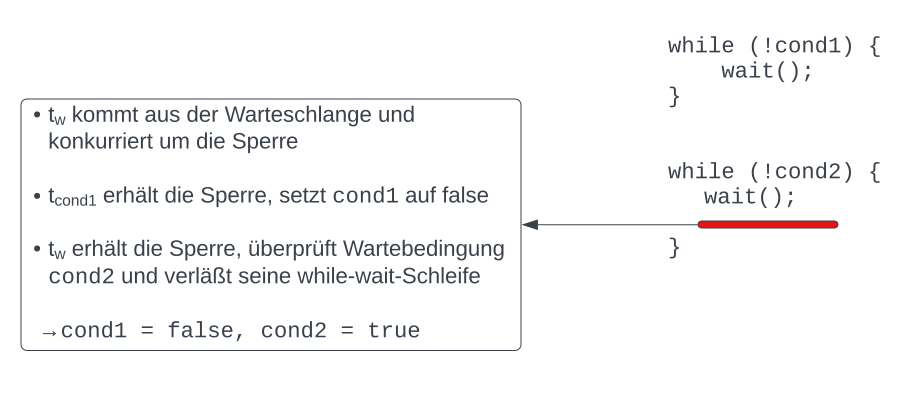
\includegraphics[scale=0.4]{chapters/Anhang/Klausuren/img/cond1cond2}
    \caption{in den rot markierten Bereich konkurriert $t_w$ um die Sperre des Objektes - wenn durch einen anderen Thread, der vor $t_w$ die Sperre erhält, \textit{cond1} auf \textit{false} gesetzt wird, stimmt die Ausgabe nicht mit der erwarteten überein. (Quelle: eigene)}
    \label{fig:cond1cond2}
\end{figure}

\noindent
Die korrekte Wartebedingung sollte lauten:

\begin{minted}[mathescape,
    linenos,
    numbersep=5pt,
    gobble=2,
    fontsize=\small,
    frame=lines,
    framesep=2mm]{java}
    public synchronized void cond1AndCond2() {
        while(!cond1 || !cond2) {
            try {
                wait();
            } catch(InterruptedException e) { }
        }
        System.out.println("cond1 and cond2:" + cond1 + " " + cond2);
    }
\end{minted}\\

Darüber hinaus müßte \code{notifyAll()} nur aufgerufen werden, wenn sowohl \code{cond1} als auch \code{cond2} auf \code{true} gesetzt sind, was leicht in den entsprechenden Methoden überprüft werden kann.
    \chapter{SS19}\label{ch:klausurss19}

\section{Aufgabe 1}

Bei der Aufgabe ist es wichtig, die Anforderungen genau zu beachten.\\
Ob eine Thread die while-wait-Schleife verlassen darf, wird von der Methode \code{tick()} gesteuert - wieviele Ticks ein Thread in der Schleife bleiben soll, wird von dem jeweiligen Thread definiert.\\
Die \code{tick()}-Methode wird von anderen Threads aufgerufen, es kann also durchaus vorkommen, dass mehrmals hintereinander
die \code{notifyAll()}-Methode aufgerufen wird - diese entfernt alle Threads aus der Warteschlange, damit die Threads ihre
Wartebedingungen erneut überprüfen können.\\
da \code{tick()} aber auch gleichzeitig einen Zähler realisieren soll, \textit{muss} es in der Methode auch eine Zählvariable geben, anhand derer die in der while-wait-Schleife enthaltenen Threads feststellen können, wie oft \code{tick()} aufgerufen wurde, um entsprechend aus der Schleife und nachfolgend der Methode herauszukommen.

\begin{figure}
    \centering
    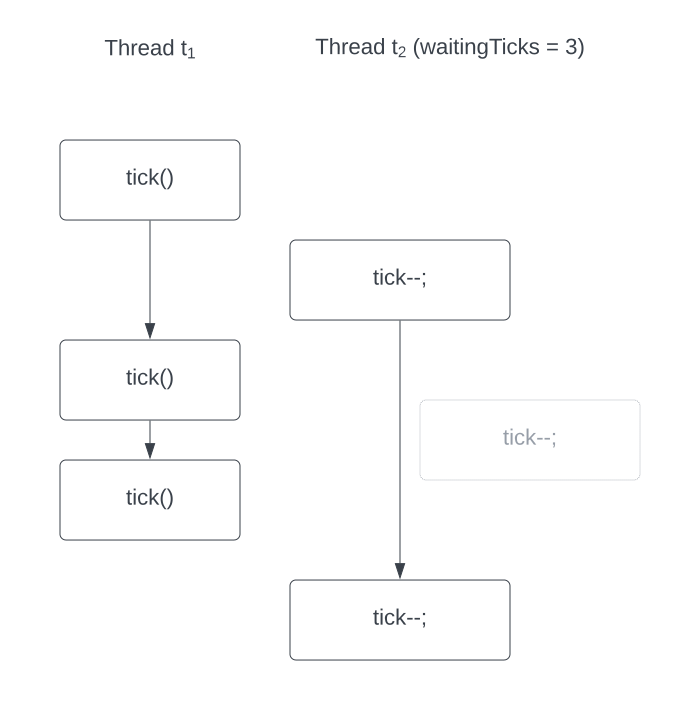
\includegraphics[scale=0.5]{chapters/Anhang/Klausuren/img/tick}
    \caption{Thread $t_1$ ruft 3 mal \texit{tick()} auf. Den Anforderungen nach müsste Thread $t_2$ danach aus der while-wait-Schleife herauskommen, erhält aber nicht die Sperre auf das Objekt von LogicalTime, um seinen eigenen Zähler rechtzeitig zu erniedrigen, bevor $t_1$ erneut \textit{tick()} aufruft. (Quelle: eigene)}
    \label{fig:tick}
\end{figure}

\section{Aufgabe 6}
Auch hier gilt, dass die Aufgabenstellung aufmerksam zu lesen ist.\\
Der Kreis soll erst ausgefüllt werden, wenn die Maustaste gelöst wird.

\begin{minted}[mathescape,
    linenos,
    numbersep=5pt,
    gobble=2,
    frame=lines,
    framesep=2mm]{java}
    private void mousePressed(double x, double y) {
        c = new Circle();
        c.setCenterX(x);
        c.setCenterY(y);
        c.setStroke(Color.RED);
        c.setFill(null); // oder Color.TRANSPARENT
        c.setRadius(RADIUS);
        graphicsPane.getChildren().add(c);
    }

    private void mouseReleased() {
        c.setFill(Color.RED);
        c = null;
    }
\end{minted}

\section{Aufgabe 8}

In der Abbildung \ref{fig:batchmodus} ist links der sequentielle Modus dargestellt, bei dem nach dem Senden einer Nachricht auf die Antwort des Servers gewartet wird, bevor eine neue Nachricht geschickt wird.
Dies wird i.d.R. verwendet, wenn das Senden einer neuen Nachricht abhängig ist von einem Ergebnis, die über die Server-Antwort übermittelt wird, oder wenn mit dem Server interagiert wird (Request abhängig vom Response).\\
Der Batch-Modus auf der rechten Seite der gleichen Abbildung ist schneller, da zwischen dem Senden von Nachrichten nicht auf Antworten gewartet werden müssen. \\
Erst nach dem Senden eine Batches von Nachrichten werden die dem Client zur Verfügung stehenden Antworten ausgelesen.\\

\noindent
In dieser Form des Batch-Modus besteht allerdings die Gefahr, dass es zu Verklemmungen kommt:
\begin{itemize}
    \item Bei dem Client kommen viele Nachrichten an, während er noch sendet.
    \item Die ankommenden Nachrichten für den Client werden gepuffert, bis sie ausgelesen werden (TCP- / OS-seitig).
    \item Läuft der Puffer voll, sorgt die Flusskontrolle (TCP) dafür, dass dem Sender mitgeteilt wird, dass keine Nachrichten mehr empfangen werden können, der Server sendet nicht mehr.
    \item Die zu sendenden Nachrichten des Servers werden in einen Puffer geschrieben.
    \item Der Sende-Puffer des Senders läuft voll.
    \item Bei dem nächsten Sende-Aufruf blockiert der Server, empfangene Nachrichten landen im Empfangspuffer
    \item Der Empfangspuffer des Servers läuft voll, der Client buffert die zu sendenden Nachrichten.
    \item Beide Anwendungen blockieren.
\end{itemize}

\\noindent
Um dieses Problem beim Batch-Modus zu umgehen, werden für das Senden und Empfangen zwei Threads auf Client-Seite erstellt: Ein Thread sendet, ein Thread empfängt. \\
Dadurch kann von dem Client immer wieder sein Empfangspuffer geleert werden, der Server wird beim Senden nicht blockiert.

\begin{figure}
    \centering
    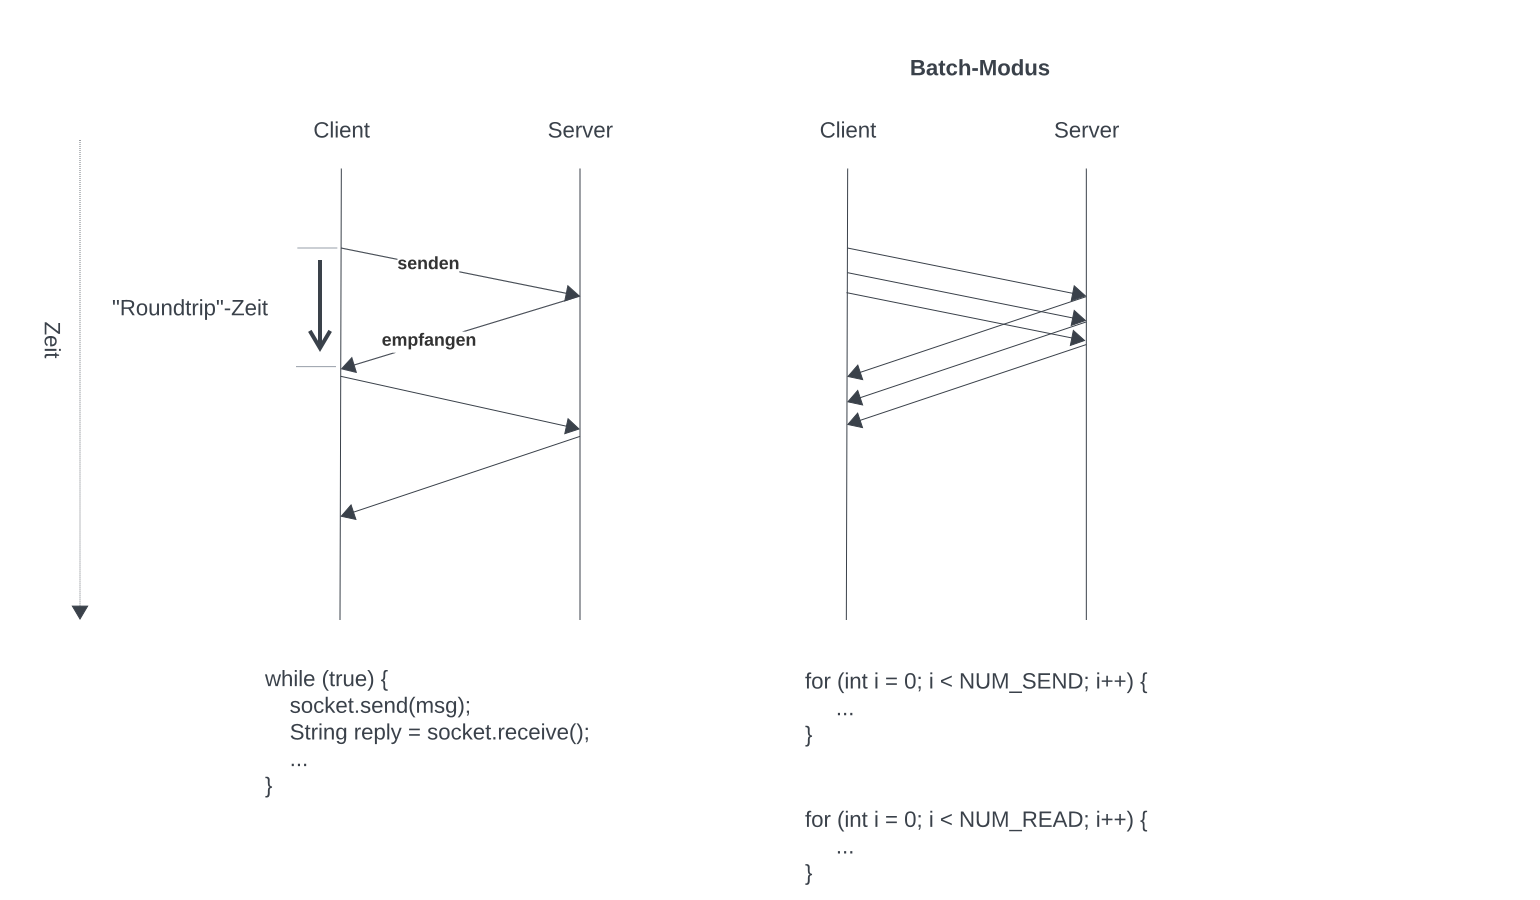
\includegraphics[scale=0.4]{chapters/Anhang/Klausuren/img/batchmodus}
    \caption{Vereinfachte Darstellung sequentieller Kommunikation und Batch-Modus (Quelle: eigene)}
    \label{fig:batchmodus}
\end{figure}
    
\begin{appendices}
    \input{chapters/Anhang/Zusatzaufgaben/index}
    \input{chapters/Anhang/Klausuren/ws13}
    \input{chapters/Anhang/Klausuren/ws15-16}
    \input{chapters/Anhang/Klausuren/ws16-17}
    \input{chapters/Anhang/Klausuren/ss19}
    \input{chapters/Anhang/Präsenzphase/index}

\end{appendices}


\end{appendices}

    \chapter{WS13}\label{ch:klausurws13}

\section{Aufgabe 1}
\subsection{Lösungsvorschlag}


\begin{minted}[mathescape,
    linenos,
    numbersep=5pt,
    gobble=2,
    fontsize=\small,
    frame=lines,
    framesep=2mm]{java}
    class Zahlenschloss {

        private int[] kombination;

        private int[] state;

        private boolean opened = false;

        public Zahlenschloss(int[] kombination) {
            this.kombination = kombination;
            this.state = new int[kombination.length];
        }

        public int anzahlRaedchen() {
            return kombination.length;
        }

        public synchronized int lesen(int radnummer) {
            return state[radnummer];
        }

        public synchronized void drehen(int radnummer, int zahl) {

            state[radnummer] = zahl;
            opened = true;
            for (int i = 0; i < anzahlRaedchen(); i++) {
                if (lesen(i) != kombination[i]) {
                    opened = false;
                    break;
                }
            }

            if (opened) {
                this.notify();
            }
        }

        public synchronized void warten() {

            while (!opened) {
                try {
                    this.wait();
                } catch (InterruptedException ignored) {}
            }
        }
    }
\end{minted}\\


\subsection{Anmerkung und Ergänzungen}

\begin{itemize}
    \item Es wird eine Wartebedingung benötigt, und zwar für die Methode \code{warten()}; ankommende Threads werden
    in die Warteschlange des Zahlenschloss-Objektes geschickt, wenn \code{opened} auf false gesetzt ist, ansonsten
    verlassen diese direkt die Methode wieder.\\
    Die Methode \code{drehen} benötigt keine separate Wartebedingung.
    Es reicht aus, sicherzustellen, dass das Zahlenschloss nicht gleichzeitig von anderen Threads benutzt werden kann:
    Die Methode \code{drehen} ist hierfür synchronisiert, damit das Zahlenschloss {insg.} immer nur eine Zustandsänderung
    erfährt - es sind andere Implementierungen möglich, in denen das Zahlenschloss dann von mehreren Threads gleichzeitig
    genutzt werden darf, wenn sich die Zugriffe anhand der ``Ziel``-\code{radnummer} unterscheiden, {bspw.} durch Mutex-Semaphore,
    die pro Radnummer verwendet werden\footnote{
        der gleichzeitige Zugriff auf unterschiedliche Arrays-Indizes ist erlaubt, s. `´17.4.1. Shared Variables``: \url{https://docs.oracle.com/javase/specs/jls/se21/html/jls-17.html#jls-1.4.1} - abgerufen 14.2.2024
    }.
    \item Es gibt nur eine Wartebedingung, von daher sollte \code{notify()} genügen.\\
    Wenn wir allerdings davon ausgehen, dass mehrere Threads über die Methode \code{warten()} in die Warteschlange des Objektes eingereiht worden sind,  sollte \code{notifyAll()} verwendet werden (siehe hierzu auch Abschnitt \ref{subsec:notifyAll}).
    Dennoch ist nicht garantiert, dass auch alle Threads aus der Warteschlange gelangen, denn es kann sein, dass ein anderer Thread die Methode \code{drehen()} betritt, dort die
    Zahlenkombination ändert und \code{opened} wieder auf \code{false} gesetzt wird. \\
    Ein anderer Thread, der nun in  \code{warten()} an die Reihe kommt, überprüft die Wartebedingung, und wird wieder in die Warteschlange eingereiht.
    Es ist also durchaus möglich, dass ein Thread nicht mehr aus der Methode \code{warten()} herauskommt.\\
    Dies könnte bspw. dadurch verhindert werden, dass die Threads in eine Queue gepackt werden, und in \code{drehen()} eine Wartebedingung eingefügt wird, die erst erfüllt ist,
    wenn die Queue geleert wurde oder aus ihr entnommen wurde, in der Reihenfolge, in der die Threads in die Queue eingereiht worden sind (\textit{FIFO}) (s. a. Abschnitt~\ref{subsec:readerwriterproblem}).
    \item Bei der Teilaufgabe mit der Schleife muss die komplette Schleife synchronisiert werden, was man durch ein \code{synchronized}-Statement erreicht\footnote{siehe Abschnitt~\ref{subsec:synchronizedstatement}.}
    \begin{minted}[mathescape,
        linenos,
        numbersep=5pt,
        gobble=2,
        fontsize=\small,
        frame=lines,
        framesep=2mm]{java}
        synchronized (zk) {
            for (int i = 0; i < anzahlRaedchen; i++) {
                System.out.println(zk.lesen(i));
            }
        }
    \end{minted}
    Ansonsten läuft man Gefahr, dass sich nach Auslesen der 1. Position der Wert von Position 2 geändert hat und dadurch eine
    Zahlenkombination ausgegeben wird, die es nicht gegeben hat:
    \begin{enumerate}
        \item $K\coloneqq[0, 0, 0]$
        \item Position $K_0$ wird ausgelesen und liefert $0$.
        \item Thread ändert $K_0$ zu $1$ $\implies K\coloneqq[1, 0, 0] $.
        \item Thread ändert $K_1$ zu $2$ $\implies K\coloneqq[1, 2, 0] $.
        \item Thread ändert $K_2$ zu $3$ $\implies K\coloneqq[1, 2, 3] $.
        \item Positionen $K_1$ und $K_2$ werden ausgelesen und liefern: $2, 3$
        \item Ausgabe: $0, 2, 3$ - diese Kombination hat es in dem Fall aber tatsächlich nicht gegeben.
    \end{enumerate}
\end{itemize}

\begin{tcolorbox}[colback=red!20,color=white,title=Anmerkung]
    Die Methode \code{lesen()} als \code{synchronized} zu markieren könnte man sich vlt. sparen, wenn man davon ausgeht,
    dass die Methode ohnehin in einem \code{synchronized}-Statement verwendet wird, um alle Rädchen abzulesen.\\
    Mehrere Threads können also nicht parallel auf unterschiedliche Positionen des Feldes zugreifen, wenn die Methode
    synchronisiert ist.\\
    Allerdings ist sowohl das Skript als auch das Buch recht klar, was in dieser Situation geschehen muss (s. Skript Fopt1/2, S. 9, außerdem \cite[31, Abschnitt 2.3.6]{Oec22}): Es muss (in diesem Kurs) immer \code{synchronized} verwendet werden, wenn gleichzeitig
    Daten geschrieben und gleichzeitig diese Daten gelesen werden sollen - und eine andere Implementierung, bei der die
    einzelnen Positionen ``gelocked`` sind, so dass ein gleichzeitiger Zugriff auf unterschiedliche Rädchen möglich ist, war nicht gefordert.\\
    Ggfl. würde in anderen Implementierungen der Einsatz von \code{AtomicReferenceArray}\footnote{s. \cite[157 ff.]{Oec22}
    s. ``Class AtomicReferenceArray<E>``: \url{https://docs.oracle.com/en/java/javase/21/docs/api/java.base/java/util/concurrent/atomic/AtomicReferenceArray.html} - abgerufen 15.2.2024
    } Sinn machen, aber das Lehrmaterial ist bereits sehr eindeutig bzgl. der Verwendung von \code{synchronized}.
\end{tcolorbox}



\section{Aufgabe 3}
\subsection{Lösungsvorschlag}

\subsection*{Statische Parallelität}
Statische Parallelität erlaubt es einem Server, eine \textit{fixe} Anzahl von Verbindungen gleichzeitig zu bedienen.\\
Hierbei wird ein Feld von Threads erstellt, wobei jeder Thread das \code{ServerSocket}-Objekt als Referenz übergeben bekommt.
In der \code{run()}-Methode wird dann über \code{accept()} in einer Endlosschleife auf eingehende Verbindungen gewartet, die dann so lange bedient werden, bis sich ein Client wieder abmeldet (oder eine andere Abbruchbedingung erfüllt ist, wie z.B. ein \code{SocketTimeout}).\\
Das sich ein Client abmeldet, bekommt man bspw. dadurch mit, dass \code{null} beim Lesen von einer Nachricht des Clients zurückgegeben wird (vgl. \cite[286]{Oec22}. \\
Siehe Abschnitt~\ref{sec:seqparserver} für ein Implementierungsbeispiel.



\subsection*{Dynamische Parallelität}

Bei der \textbf{Dynamischer Parallelität} erzeugt der Server für jede Verbindung einen neuen Thread, der so lange läuft, bis der Client die Verbindung wieder trennt.\\
Die Anzahl der Threads ändert sich dadurch laufend.\\
Wird die max. Anzahl erlaubter Threads nicht kontrolliert, kann es zu einer Überlastung des Server-Rechners kommen (bspw. durch einen Denial-of-Service-Angriff.)\\

\noindent
I.d.R. ist eine Mischform aus beidem geeignet, um mehrere Clients gleichzeitig bedienen zu können, und dabei nicht Gefahr zu laufen, durch dynamisches, unbegrenztes Wachstum der Anzahl der Threads überlastet zu werden.

    \chapter{WS13}\label{ch:klausurws5-16}

\section{Rechteck-Scroll (SS15 Aufgabe 2)}

Aufgabenstellung unklar.\\
Mögliche Implementierung unter \url{https://github.com/ThorstenSuckow/fopt/tree/main/src/main/java/klausurvorbereitung/foptws1516/MouseDragsSquareDemo}.

\section{Rechteck-Scroll (WS15/16 Aufgabe 1)}

Aufgabenstellung unklar.\\
Mögliche Implementierung unter \url{https://github.com/ThorstenSuckow/fopt/tree/main/src/main/java/klausurvorbereitung/foptws1516/MaxWeightDemo}.\\

\noindent
Es gibt nur eine Warteschlange für Threads in \code{use()}, es gibt keine Wartebedingung in \code{dontUse()} und damit auch keine weitere Warteschlange.\\
Es sind durch die Zugriffe auf unterschiedliche Indizes allerdings mehrere Wartebedingungen vorhanden, weshalb hab \code{notifyAll()} nutzen sollte,
sobald ein Zugriff auf ein Feld nach Aufruf von \code{dontUse} wieder möglich wird.\\
Ansonsten bestünde die Gefahr, dass bei dem Einsatz von \code{notify()} ein wartender Thread nicht geweckt wird, obwohl er weiterlaufen könnte:\\
Angenommen, das Feld $F$ hat eine Länge von $3$, das \code{maxWeight} ist mit $2$ konfiguriert.
Thread $t_1$ mit einer Laufzeit von $200\ sek$ bekommt Zugriff auf $F_0$, setzt $currentWeight$ auf $1$.\\
Thread $t_2$ mit einer Laufzeit von $1\ sek$ möchte auf $F_1$ zugreifen, setzt $currentWeight=2$ in die Warteschlange.\\
Thread $t_3$ meldet Zugriff auf $F_0$ an und gelangt in die Warteschlange.\\
Thread $t_4$ meldet Zugriff auf $F_1$ an und gelangt in die Warteschlange.\\
Thread $t_2$ ist mit der Bearbeitung von $F_1$ fertig, $currentWeight$ wird auf $1$ gesetzt, \code{notify()} wird aufgerufen.\\
Thread $t_3$ wird aus der Warteschlange geholt, kann aber nicht weiterarbeiten, da $F_0$ noch durch den länger dauernden $t_1$ blockiert ist, und kommt wieder in die Warteschlange.\\

\noindent
Offensichtlich hätte in dem Beispiel \code{notifyAll()} dazu geführt, dass auch $T_4$ seine Wartebedingung hätte überprüfen können, und hätte so Zugriff auf $F_1$ bekommen.
Stattdessen muss nun gewartet werden, bis das nächste \code{notify()} aufgerufen wird, oder ein neu ankommender Thread $F_1$ belegt.

    \chapter{WS16-17}\label{ch:klausurws16-17}

\section{Aufgabe 1}
\subsection{Lösungshinweis}

Die erste Aufgabe verdeutlicht, was bei einem \code{notifyAll()} und unsauber gesetzten Wartebedingungen passieren kann.\\
Sei folgender Quellcode gegeben:


\begin{minted}[mathescape,
    linenos,
    numbersep=5pt,
    gobble=2,
    fontsize=\small,
    frame=lines,
    framesep=2mm]{java}
    class Cond1AndCond2 {

        private boolean cond1;
        private boolean cond2;

        public synchronized void setCond1(boolean c) {
            cond1 = c;
            notifyAll();
        }

        public synchronized void setCond2(boolean c) {
            cond2 = c;
            notifyAll();
        }

        public synchronized void cond1AndCond2() {
            while(!cond1) {
                try {
                    wait();
                } catch(InterruptedException e) { }
            }

            while(!cond2) {
                try {
                    wait();
                } catch(InterruptedException e) {}
            }
            System.out.println("cond1 and cond2:" + cond1 + " " + cond2);
        }
    }
\end{minted}\\

Man sollte auf den ersten Blick meinen, dass \code{cond1} und \code{cond2} beide \code{true} sein müssen, damit die Ausgabe erfolgt.\\
Tatsächlich ist es aber so, dass es in der Methode zwei unterschiedliche Wartebedingungen gibt.\\
Die erste Wartebedingung schickt einen Thread in die Warteschlange, wenn \code{cond1 == false} gilt.\\
Setzt ein anderer Thread über \code{setCond1(true)} das Attribut entsprechend auf \code{true}, bewirkt der nachfolgende Aufruf von \code{notifyAll()}, dass alle \textit{wartenden} Threads aus der Warteschlange entfernt werden und erneut um eine Sperre des Objektes konkurrieren.\\
Erhält ein entsprechender Thread $t_w$ die Sperre auf das Objekt und kann seine \textit{while-wait-Schleife} verlassen, kann es vorkommen, dass er erneut in die Warteschlange eingereiht wird, wegen der nachfolgenden Wartebedingung \code{cond2 == false}.\\
Angenommen, ein weiterer Thread ruft nun \code{setCond2(true)} auf, und $t_w$ kommt aus der Warteschlange und konkurriert erneut und um die Sperre des Objektes, dann kann es vorkommen, das ein anderer Thread zunächst die Sperre erhält, \code{cond1} wieder auf \code{false} setzt, dann erhält $t_w$ die Sperre, überprüft die Wartebedingung \code{cond2 == false}.\\
Wegen \code{cond2} gelangt er aus der \textit{while-wait-Schleife} und die Ausgabe erfolgt - da zwischenzeitlich \code{cond1} wieder auf \code{false} gesetzt wurde, ist die erwartete Ausgabe nicht \code{true true}, sondern \code{false true} (s. Abbildung \ref{fig:cond1cond2}).\\

\begin{figure}
    \centering
    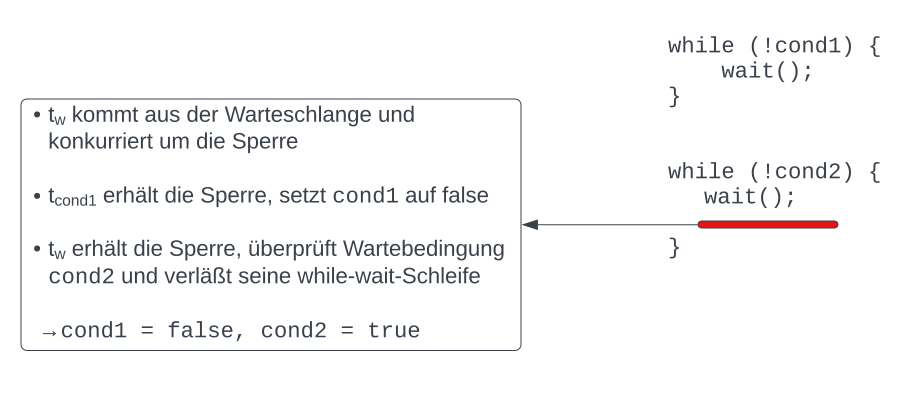
\includegraphics[scale=0.4]{chapters/Anhang/Klausuren/img/cond1cond2}
    \caption{in den rot markierten Bereich konkurriert $t_w$ um die Sperre des Objektes - wenn durch einen anderen Thread, der vor $t_w$ die Sperre erhält, \textit{cond1} auf \textit{false} gesetzt wird, stimmt die Ausgabe nicht mit der erwarteten überein. (Quelle: eigene)}
    \label{fig:cond1cond2}
\end{figure}

\noindent
Die korrekte Wartebedingung sollte lauten:

\begin{minted}[mathescape,
    linenos,
    numbersep=5pt,
    gobble=2,
    fontsize=\small,
    frame=lines,
    framesep=2mm]{java}
    public synchronized void cond1AndCond2() {
        while(!cond1 || !cond2) {
            try {
                wait();
            } catch(InterruptedException e) { }
        }
        System.out.println("cond1 and cond2:" + cond1 + " " + cond2);
    }
\end{minted}\\

Darüber hinaus müßte \code{notifyAll()} nur aufgerufen werden, wenn sowohl \code{cond1} als auch \code{cond2} auf \code{true} gesetzt sind, was leicht in den entsprechenden Methoden überprüft werden kann.
    \chapter{SS19}\label{ch:klausurss19}

\section{Aufgabe 1}

Bei der Aufgabe ist es wichtig, die Anforderungen genau zu beachten.\\
Ob eine Thread die while-wait-Schleife verlassen darf, wird von der Methode \code{tick()} gesteuert - wieviele Ticks ein Thread in der Schleife bleiben soll, wird von dem jeweiligen Thread definiert.\\
Die \code{tick()}-Methode wird von anderen Threads aufgerufen, es kann also durchaus vorkommen, dass mehrmals hintereinander
die \code{notifyAll()}-Methode aufgerufen wird - diese entfernt alle Threads aus der Warteschlange, damit die Threads ihre
Wartebedingungen erneut überprüfen können.\\
da \code{tick()} aber auch gleichzeitig einen Zähler realisieren soll, \textit{muss} es in der Methode auch eine Zählvariable geben, anhand derer die in der while-wait-Schleife enthaltenen Threads feststellen können, wie oft \code{tick()} aufgerufen wurde, um entsprechend aus der Schleife und nachfolgend der Methode herauszukommen.

\begin{figure}
    \centering
    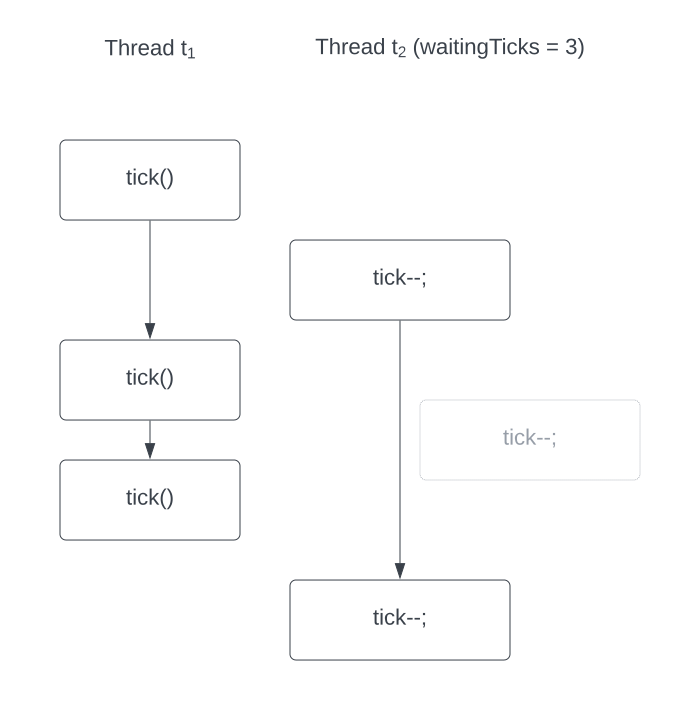
\includegraphics[scale=0.5]{chapters/Anhang/Klausuren/img/tick}
    \caption{Thread $t_1$ ruft 3 mal \texit{tick()} auf. Den Anforderungen nach müsste Thread $t_2$ danach aus der while-wait-Schleife herauskommen, erhält aber nicht die Sperre auf das Objekt von LogicalTime, um seinen eigenen Zähler rechtzeitig zu erniedrigen, bevor $t_1$ erneut \textit{tick()} aufruft. (Quelle: eigene)}
    \label{fig:tick}
\end{figure}

\section{Aufgabe 6}
Auch hier gilt, dass die Aufgabenstellung aufmerksam zu lesen ist.\\
Der Kreis soll erst ausgefüllt werden, wenn die Maustaste gelöst wird.

\begin{minted}[mathescape,
    linenos,
    numbersep=5pt,
    gobble=2,
    frame=lines,
    framesep=2mm]{java}
    private void mousePressed(double x, double y) {
        c = new Circle();
        c.setCenterX(x);
        c.setCenterY(y);
        c.setStroke(Color.RED);
        c.setFill(null); // oder Color.TRANSPARENT
        c.setRadius(RADIUS);
        graphicsPane.getChildren().add(c);
    }

    private void mouseReleased() {
        c.setFill(Color.RED);
        c = null;
    }
\end{minted}

\section{Aufgabe 8}

In der Abbildung \ref{fig:batchmodus} ist links der sequentielle Modus dargestellt, bei dem nach dem Senden einer Nachricht auf die Antwort des Servers gewartet wird, bevor eine neue Nachricht geschickt wird.
Dies wird i.d.R. verwendet, wenn das Senden einer neuen Nachricht abhängig ist von einem Ergebnis, die über die Server-Antwort übermittelt wird, oder wenn mit dem Server interagiert wird (Request abhängig vom Response).\\
Der Batch-Modus auf der rechten Seite der gleichen Abbildung ist schneller, da zwischen dem Senden von Nachrichten nicht auf Antworten gewartet werden müssen. \\
Erst nach dem Senden eine Batches von Nachrichten werden die dem Client zur Verfügung stehenden Antworten ausgelesen.\\

\noindent
In dieser Form des Batch-Modus besteht allerdings die Gefahr, dass es zu Verklemmungen kommt:
\begin{itemize}
    \item Bei dem Client kommen viele Nachrichten an, während er noch sendet.
    \item Die ankommenden Nachrichten für den Client werden gepuffert, bis sie ausgelesen werden (TCP- / OS-seitig).
    \item Läuft der Puffer voll, sorgt die Flusskontrolle (TCP) dafür, dass dem Sender mitgeteilt wird, dass keine Nachrichten mehr empfangen werden können, der Server sendet nicht mehr.
    \item Die zu sendenden Nachrichten des Servers werden in einen Puffer geschrieben.
    \item Der Sende-Puffer des Senders läuft voll.
    \item Bei dem nächsten Sende-Aufruf blockiert der Server, empfangene Nachrichten landen im Empfangspuffer
    \item Der Empfangspuffer des Servers läuft voll, der Client buffert die zu sendenden Nachrichten.
    \item Beide Anwendungen blockieren.
\end{itemize}

\\noindent
Um dieses Problem beim Batch-Modus zu umgehen, werden für das Senden und Empfangen zwei Threads auf Client-Seite erstellt: Ein Thread sendet, ein Thread empfängt. \\
Dadurch kann von dem Client immer wieder sein Empfangspuffer geleert werden, der Server wird beim Senden nicht blockiert.

\begin{figure}
    \centering
    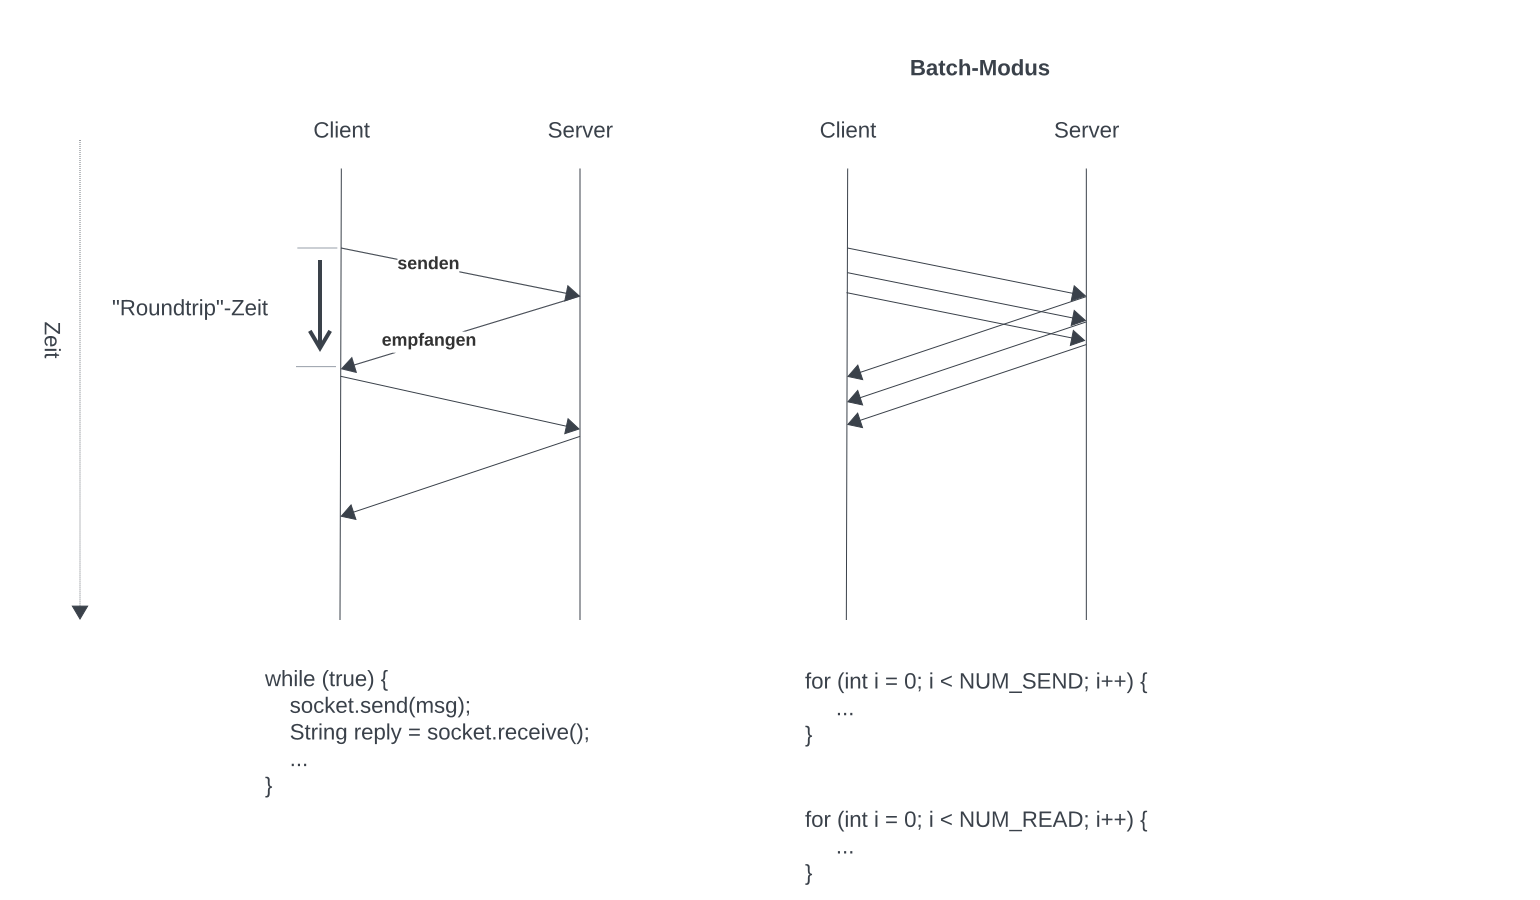
\includegraphics[scale=0.4]{chapters/Anhang/Klausuren/img/batchmodus}
    \caption{Vereinfachte Darstellung sequentieller Kommunikation und Batch-Modus (Quelle: eigene)}
    \label{fig:batchmodus}
\end{figure}
    
\begin{appendices}
    
\begin{appendices}
    \input{chapters/Anhang/Zusatzaufgaben/index}
    \input{chapters/Anhang/Klausuren/ws13}
    \input{chapters/Anhang/Klausuren/ws15-16}
    \input{chapters/Anhang/Klausuren/ws16-17}
    \input{chapters/Anhang/Klausuren/ss19}
    \input{chapters/Anhang/Präsenzphase/index}

\end{appendices}

    \chapter{WS13}\label{ch:klausurws13}

\section{Aufgabe 1}
\subsection{Lösungsvorschlag}


\begin{minted}[mathescape,
    linenos,
    numbersep=5pt,
    gobble=2,
    fontsize=\small,
    frame=lines,
    framesep=2mm]{java}
    class Zahlenschloss {

        private int[] kombination;

        private int[] state;

        private boolean opened = false;

        public Zahlenschloss(int[] kombination) {
            this.kombination = kombination;
            this.state = new int[kombination.length];
        }

        public int anzahlRaedchen() {
            return kombination.length;
        }

        public synchronized int lesen(int radnummer) {
            return state[radnummer];
        }

        public synchronized void drehen(int radnummer, int zahl) {

            state[radnummer] = zahl;
            opened = true;
            for (int i = 0; i < anzahlRaedchen(); i++) {
                if (lesen(i) != kombination[i]) {
                    opened = false;
                    break;
                }
            }

            if (opened) {
                this.notify();
            }
        }

        public synchronized void warten() {

            while (!opened) {
                try {
                    this.wait();
                } catch (InterruptedException ignored) {}
            }
        }
    }
\end{minted}\\


\subsection{Anmerkung und Ergänzungen}

\begin{itemize}
    \item Es wird eine Wartebedingung benötigt, und zwar für die Methode \code{warten()}; ankommende Threads werden
    in die Warteschlange des Zahlenschloss-Objektes geschickt, wenn \code{opened} auf false gesetzt ist, ansonsten
    verlassen diese direkt die Methode wieder.\\
    Die Methode \code{drehen} benötigt keine separate Wartebedingung.
    Es reicht aus, sicherzustellen, dass das Zahlenschloss nicht gleichzeitig von anderen Threads benutzt werden kann:
    Die Methode \code{drehen} ist hierfür synchronisiert, damit das Zahlenschloss {insg.} immer nur eine Zustandsänderung
    erfährt - es sind andere Implementierungen möglich, in denen das Zahlenschloss dann von mehreren Threads gleichzeitig
    genutzt werden darf, wenn sich die Zugriffe anhand der ``Ziel``-\code{radnummer} unterscheiden, {bspw.} durch Mutex-Semaphore,
    die pro Radnummer verwendet werden\footnote{
        der gleichzeitige Zugriff auf unterschiedliche Arrays-Indizes ist erlaubt, s. `´17.4.1. Shared Variables``: \url{https://docs.oracle.com/javase/specs/jls/se21/html/jls-17.html#jls-1.4.1} - abgerufen 14.2.2024
    }.
    \item Es gibt nur eine Wartebedingung, von daher sollte \code{notify()} genügen.\\
    Wenn wir allerdings davon ausgehen, dass mehrere Threads über die Methode \code{warten()} in die Warteschlange des Objektes eingereiht worden sind,  sollte \code{notifyAll()} verwendet werden (siehe hierzu auch Abschnitt \ref{subsec:notifyAll}).
    Dennoch ist nicht garantiert, dass auch alle Threads aus der Warteschlange gelangen, denn es kann sein, dass ein anderer Thread die Methode \code{drehen()} betritt, dort die
    Zahlenkombination ändert und \code{opened} wieder auf \code{false} gesetzt wird. \\
    Ein anderer Thread, der nun in  \code{warten()} an die Reihe kommt, überprüft die Wartebedingung, und wird wieder in die Warteschlange eingereiht.
    Es ist also durchaus möglich, dass ein Thread nicht mehr aus der Methode \code{warten()} herauskommt.\\
    Dies könnte bspw. dadurch verhindert werden, dass die Threads in eine Queue gepackt werden, und in \code{drehen()} eine Wartebedingung eingefügt wird, die erst erfüllt ist,
    wenn die Queue geleert wurde oder aus ihr entnommen wurde, in der Reihenfolge, in der die Threads in die Queue eingereiht worden sind (\textit{FIFO}) (s. a. Abschnitt~\ref{subsec:readerwriterproblem}).
    \item Bei der Teilaufgabe mit der Schleife muss die komplette Schleife synchronisiert werden, was man durch ein \code{synchronized}-Statement erreicht\footnote{siehe Abschnitt~\ref{subsec:synchronizedstatement}.}
    \begin{minted}[mathescape,
        linenos,
        numbersep=5pt,
        gobble=2,
        fontsize=\small,
        frame=lines,
        framesep=2mm]{java}
        synchronized (zk) {
            for (int i = 0; i < anzahlRaedchen; i++) {
                System.out.println(zk.lesen(i));
            }
        }
    \end{minted}
    Ansonsten läuft man Gefahr, dass sich nach Auslesen der 1. Position der Wert von Position 2 geändert hat und dadurch eine
    Zahlenkombination ausgegeben wird, die es nicht gegeben hat:
    \begin{enumerate}
        \item $K\coloneqq[0, 0, 0]$
        \item Position $K_0$ wird ausgelesen und liefert $0$.
        \item Thread ändert $K_0$ zu $1$ $\implies K\coloneqq[1, 0, 0] $.
        \item Thread ändert $K_1$ zu $2$ $\implies K\coloneqq[1, 2, 0] $.
        \item Thread ändert $K_2$ zu $3$ $\implies K\coloneqq[1, 2, 3] $.
        \item Positionen $K_1$ und $K_2$ werden ausgelesen und liefern: $2, 3$
        \item Ausgabe: $0, 2, 3$ - diese Kombination hat es in dem Fall aber tatsächlich nicht gegeben.
    \end{enumerate}
\end{itemize}

\begin{tcolorbox}[colback=red!20,color=white,title=Anmerkung]
    Die Methode \code{lesen()} als \code{synchronized} zu markieren könnte man sich vlt. sparen, wenn man davon ausgeht,
    dass die Methode ohnehin in einem \code{synchronized}-Statement verwendet wird, um alle Rädchen abzulesen.\\
    Mehrere Threads können also nicht parallel auf unterschiedliche Positionen des Feldes zugreifen, wenn die Methode
    synchronisiert ist.\\
    Allerdings ist sowohl das Skript als auch das Buch recht klar, was in dieser Situation geschehen muss (s. Skript Fopt1/2, S. 9, außerdem \cite[31, Abschnitt 2.3.6]{Oec22}): Es muss (in diesem Kurs) immer \code{synchronized} verwendet werden, wenn gleichzeitig
    Daten geschrieben und gleichzeitig diese Daten gelesen werden sollen - und eine andere Implementierung, bei der die
    einzelnen Positionen ``gelocked`` sind, so dass ein gleichzeitiger Zugriff auf unterschiedliche Rädchen möglich ist, war nicht gefordert.\\
    Ggfl. würde in anderen Implementierungen der Einsatz von \code{AtomicReferenceArray}\footnote{s. \cite[157 ff.]{Oec22}
    s. ``Class AtomicReferenceArray<E>``: \url{https://docs.oracle.com/en/java/javase/21/docs/api/java.base/java/util/concurrent/atomic/AtomicReferenceArray.html} - abgerufen 15.2.2024
    } Sinn machen, aber das Lehrmaterial ist bereits sehr eindeutig bzgl. der Verwendung von \code{synchronized}.
\end{tcolorbox}



\section{Aufgabe 3}
\subsection{Lösungsvorschlag}

\subsection*{Statische Parallelität}
Statische Parallelität erlaubt es einem Server, eine \textit{fixe} Anzahl von Verbindungen gleichzeitig zu bedienen.\\
Hierbei wird ein Feld von Threads erstellt, wobei jeder Thread das \code{ServerSocket}-Objekt als Referenz übergeben bekommt.
In der \code{run()}-Methode wird dann über \code{accept()} in einer Endlosschleife auf eingehende Verbindungen gewartet, die dann so lange bedient werden, bis sich ein Client wieder abmeldet (oder eine andere Abbruchbedingung erfüllt ist, wie z.B. ein \code{SocketTimeout}).\\
Das sich ein Client abmeldet, bekommt man bspw. dadurch mit, dass \code{null} beim Lesen von einer Nachricht des Clients zurückgegeben wird (vgl. \cite[286]{Oec22}. \\
Siehe Abschnitt~\ref{sec:seqparserver} für ein Implementierungsbeispiel.



\subsection*{Dynamische Parallelität}

Bei der \textbf{Dynamischer Parallelität} erzeugt der Server für jede Verbindung einen neuen Thread, der so lange läuft, bis der Client die Verbindung wieder trennt.\\
Die Anzahl der Threads ändert sich dadurch laufend.\\
Wird die max. Anzahl erlaubter Threads nicht kontrolliert, kann es zu einer Überlastung des Server-Rechners kommen (bspw. durch einen Denial-of-Service-Angriff.)\\

\noindent
I.d.R. ist eine Mischform aus beidem geeignet, um mehrere Clients gleichzeitig bedienen zu können, und dabei nicht Gefahr zu laufen, durch dynamisches, unbegrenztes Wachstum der Anzahl der Threads überlastet zu werden.

    \chapter{WS13}\label{ch:klausurws5-16}

\section{Rechteck-Scroll (SS15 Aufgabe 2)}

Aufgabenstellung unklar.\\
Mögliche Implementierung unter \url{https://github.com/ThorstenSuckow/fopt/tree/main/src/main/java/klausurvorbereitung/foptws1516/MouseDragsSquareDemo}.

\section{Rechteck-Scroll (WS15/16 Aufgabe 1)}

Aufgabenstellung unklar.\\
Mögliche Implementierung unter \url{https://github.com/ThorstenSuckow/fopt/tree/main/src/main/java/klausurvorbereitung/foptws1516/MaxWeightDemo}.\\

\noindent
Es gibt nur eine Warteschlange für Threads in \code{use()}, es gibt keine Wartebedingung in \code{dontUse()} und damit auch keine weitere Warteschlange.\\
Es sind durch die Zugriffe auf unterschiedliche Indizes allerdings mehrere Wartebedingungen vorhanden, weshalb hab \code{notifyAll()} nutzen sollte,
sobald ein Zugriff auf ein Feld nach Aufruf von \code{dontUse} wieder möglich wird.\\
Ansonsten bestünde die Gefahr, dass bei dem Einsatz von \code{notify()} ein wartender Thread nicht geweckt wird, obwohl er weiterlaufen könnte:\\
Angenommen, das Feld $F$ hat eine Länge von $3$, das \code{maxWeight} ist mit $2$ konfiguriert.
Thread $t_1$ mit einer Laufzeit von $200\ sek$ bekommt Zugriff auf $F_0$, setzt $currentWeight$ auf $1$.\\
Thread $t_2$ mit einer Laufzeit von $1\ sek$ möchte auf $F_1$ zugreifen, setzt $currentWeight=2$ in die Warteschlange.\\
Thread $t_3$ meldet Zugriff auf $F_0$ an und gelangt in die Warteschlange.\\
Thread $t_4$ meldet Zugriff auf $F_1$ an und gelangt in die Warteschlange.\\
Thread $t_2$ ist mit der Bearbeitung von $F_1$ fertig, $currentWeight$ wird auf $1$ gesetzt, \code{notify()} wird aufgerufen.\\
Thread $t_3$ wird aus der Warteschlange geholt, kann aber nicht weiterarbeiten, da $F_0$ noch durch den länger dauernden $t_1$ blockiert ist, und kommt wieder in die Warteschlange.\\

\noindent
Offensichtlich hätte in dem Beispiel \code{notifyAll()} dazu geführt, dass auch $T_4$ seine Wartebedingung hätte überprüfen können, und hätte so Zugriff auf $F_1$ bekommen.
Stattdessen muss nun gewartet werden, bis das nächste \code{notify()} aufgerufen wird, oder ein neu ankommender Thread $F_1$ belegt.

    \chapter{WS16-17}\label{ch:klausurws16-17}

\section{Aufgabe 1}
\subsection{Lösungshinweis}

Die erste Aufgabe verdeutlicht, was bei einem \code{notifyAll()} und unsauber gesetzten Wartebedingungen passieren kann.\\
Sei folgender Quellcode gegeben:


\begin{minted}[mathescape,
    linenos,
    numbersep=5pt,
    gobble=2,
    fontsize=\small,
    frame=lines,
    framesep=2mm]{java}
    class Cond1AndCond2 {

        private boolean cond1;
        private boolean cond2;

        public synchronized void setCond1(boolean c) {
            cond1 = c;
            notifyAll();
        }

        public synchronized void setCond2(boolean c) {
            cond2 = c;
            notifyAll();
        }

        public synchronized void cond1AndCond2() {
            while(!cond1) {
                try {
                    wait();
                } catch(InterruptedException e) { }
            }

            while(!cond2) {
                try {
                    wait();
                } catch(InterruptedException e) {}
            }
            System.out.println("cond1 and cond2:" + cond1 + " " + cond2);
        }
    }
\end{minted}\\

Man sollte auf den ersten Blick meinen, dass \code{cond1} und \code{cond2} beide \code{true} sein müssen, damit die Ausgabe erfolgt.\\
Tatsächlich ist es aber so, dass es in der Methode zwei unterschiedliche Wartebedingungen gibt.\\
Die erste Wartebedingung schickt einen Thread in die Warteschlange, wenn \code{cond1 == false} gilt.\\
Setzt ein anderer Thread über \code{setCond1(true)} das Attribut entsprechend auf \code{true}, bewirkt der nachfolgende Aufruf von \code{notifyAll()}, dass alle \textit{wartenden} Threads aus der Warteschlange entfernt werden und erneut um eine Sperre des Objektes konkurrieren.\\
Erhält ein entsprechender Thread $t_w$ die Sperre auf das Objekt und kann seine \textit{while-wait-Schleife} verlassen, kann es vorkommen, dass er erneut in die Warteschlange eingereiht wird, wegen der nachfolgenden Wartebedingung \code{cond2 == false}.\\
Angenommen, ein weiterer Thread ruft nun \code{setCond2(true)} auf, und $t_w$ kommt aus der Warteschlange und konkurriert erneut und um die Sperre des Objektes, dann kann es vorkommen, das ein anderer Thread zunächst die Sperre erhält, \code{cond1} wieder auf \code{false} setzt, dann erhält $t_w$ die Sperre, überprüft die Wartebedingung \code{cond2 == false}.\\
Wegen \code{cond2} gelangt er aus der \textit{while-wait-Schleife} und die Ausgabe erfolgt - da zwischenzeitlich \code{cond1} wieder auf \code{false} gesetzt wurde, ist die erwartete Ausgabe nicht \code{true true}, sondern \code{false true} (s. Abbildung \ref{fig:cond1cond2}).\\

\begin{figure}
    \centering
    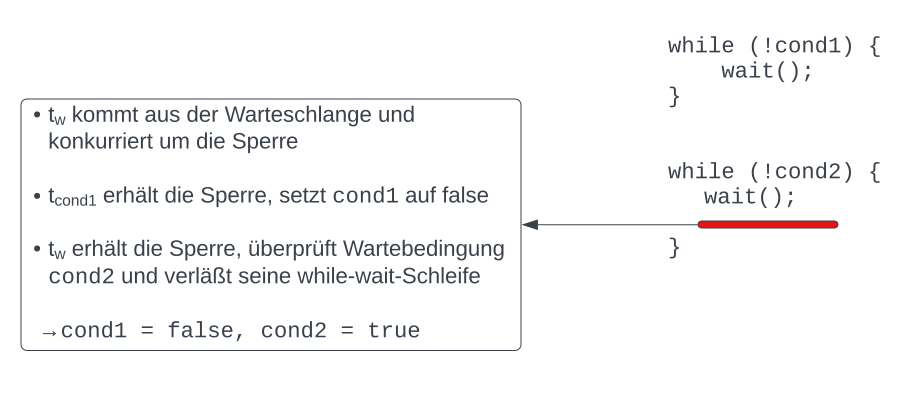
\includegraphics[scale=0.4]{chapters/Anhang/Klausuren/img/cond1cond2}
    \caption{in den rot markierten Bereich konkurriert $t_w$ um die Sperre des Objektes - wenn durch einen anderen Thread, der vor $t_w$ die Sperre erhält, \textit{cond1} auf \textit{false} gesetzt wird, stimmt die Ausgabe nicht mit der erwarteten überein. (Quelle: eigene)}
    \label{fig:cond1cond2}
\end{figure}

\noindent
Die korrekte Wartebedingung sollte lauten:

\begin{minted}[mathescape,
    linenos,
    numbersep=5pt,
    gobble=2,
    fontsize=\small,
    frame=lines,
    framesep=2mm]{java}
    public synchronized void cond1AndCond2() {
        while(!cond1 || !cond2) {
            try {
                wait();
            } catch(InterruptedException e) { }
        }
        System.out.println("cond1 and cond2:" + cond1 + " " + cond2);
    }
\end{minted}\\

Darüber hinaus müßte \code{notifyAll()} nur aufgerufen werden, wenn sowohl \code{cond1} als auch \code{cond2} auf \code{true} gesetzt sind, was leicht in den entsprechenden Methoden überprüft werden kann.
    \chapter{SS19}\label{ch:klausurss19}

\section{Aufgabe 1}

Bei der Aufgabe ist es wichtig, die Anforderungen genau zu beachten.\\
Ob eine Thread die while-wait-Schleife verlassen darf, wird von der Methode \code{tick()} gesteuert - wieviele Ticks ein Thread in der Schleife bleiben soll, wird von dem jeweiligen Thread definiert.\\
Die \code{tick()}-Methode wird von anderen Threads aufgerufen, es kann also durchaus vorkommen, dass mehrmals hintereinander
die \code{notifyAll()}-Methode aufgerufen wird - diese entfernt alle Threads aus der Warteschlange, damit die Threads ihre
Wartebedingungen erneut überprüfen können.\\
da \code{tick()} aber auch gleichzeitig einen Zähler realisieren soll, \textit{muss} es in der Methode auch eine Zählvariable geben, anhand derer die in der while-wait-Schleife enthaltenen Threads feststellen können, wie oft \code{tick()} aufgerufen wurde, um entsprechend aus der Schleife und nachfolgend der Methode herauszukommen.

\begin{figure}
    \centering
    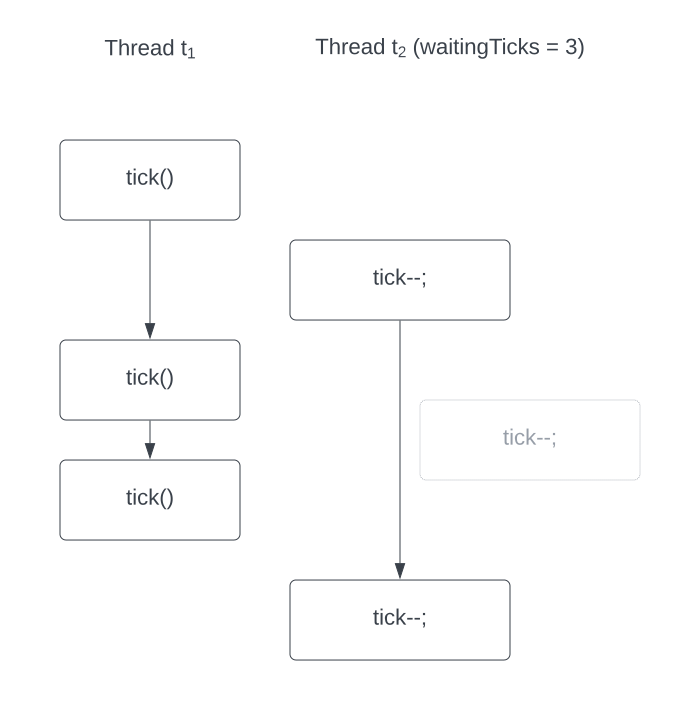
\includegraphics[scale=0.5]{chapters/Anhang/Klausuren/img/tick}
    \caption{Thread $t_1$ ruft 3 mal \texit{tick()} auf. Den Anforderungen nach müsste Thread $t_2$ danach aus der while-wait-Schleife herauskommen, erhält aber nicht die Sperre auf das Objekt von LogicalTime, um seinen eigenen Zähler rechtzeitig zu erniedrigen, bevor $t_1$ erneut \textit{tick()} aufruft. (Quelle: eigene)}
    \label{fig:tick}
\end{figure}

\section{Aufgabe 6}
Auch hier gilt, dass die Aufgabenstellung aufmerksam zu lesen ist.\\
Der Kreis soll erst ausgefüllt werden, wenn die Maustaste gelöst wird.

\begin{minted}[mathescape,
    linenos,
    numbersep=5pt,
    gobble=2,
    frame=lines,
    framesep=2mm]{java}
    private void mousePressed(double x, double y) {
        c = new Circle();
        c.setCenterX(x);
        c.setCenterY(y);
        c.setStroke(Color.RED);
        c.setFill(null); // oder Color.TRANSPARENT
        c.setRadius(RADIUS);
        graphicsPane.getChildren().add(c);
    }

    private void mouseReleased() {
        c.setFill(Color.RED);
        c = null;
    }
\end{minted}

\section{Aufgabe 8}

In der Abbildung \ref{fig:batchmodus} ist links der sequentielle Modus dargestellt, bei dem nach dem Senden einer Nachricht auf die Antwort des Servers gewartet wird, bevor eine neue Nachricht geschickt wird.
Dies wird i.d.R. verwendet, wenn das Senden einer neuen Nachricht abhängig ist von einem Ergebnis, die über die Server-Antwort übermittelt wird, oder wenn mit dem Server interagiert wird (Request abhängig vom Response).\\
Der Batch-Modus auf der rechten Seite der gleichen Abbildung ist schneller, da zwischen dem Senden von Nachrichten nicht auf Antworten gewartet werden müssen. \\
Erst nach dem Senden eine Batches von Nachrichten werden die dem Client zur Verfügung stehenden Antworten ausgelesen.\\

\noindent
In dieser Form des Batch-Modus besteht allerdings die Gefahr, dass es zu Verklemmungen kommt:
\begin{itemize}
    \item Bei dem Client kommen viele Nachrichten an, während er noch sendet.
    \item Die ankommenden Nachrichten für den Client werden gepuffert, bis sie ausgelesen werden (TCP- / OS-seitig).
    \item Läuft der Puffer voll, sorgt die Flusskontrolle (TCP) dafür, dass dem Sender mitgeteilt wird, dass keine Nachrichten mehr empfangen werden können, der Server sendet nicht mehr.
    \item Die zu sendenden Nachrichten des Servers werden in einen Puffer geschrieben.
    \item Der Sende-Puffer des Senders läuft voll.
    \item Bei dem nächsten Sende-Aufruf blockiert der Server, empfangene Nachrichten landen im Empfangspuffer
    \item Der Empfangspuffer des Servers läuft voll, der Client buffert die zu sendenden Nachrichten.
    \item Beide Anwendungen blockieren.
\end{itemize}

\\noindent
Um dieses Problem beim Batch-Modus zu umgehen, werden für das Senden und Empfangen zwei Threads auf Client-Seite erstellt: Ein Thread sendet, ein Thread empfängt. \\
Dadurch kann von dem Client immer wieder sein Empfangspuffer geleert werden, der Server wird beim Senden nicht blockiert.

\begin{figure}
    \centering
    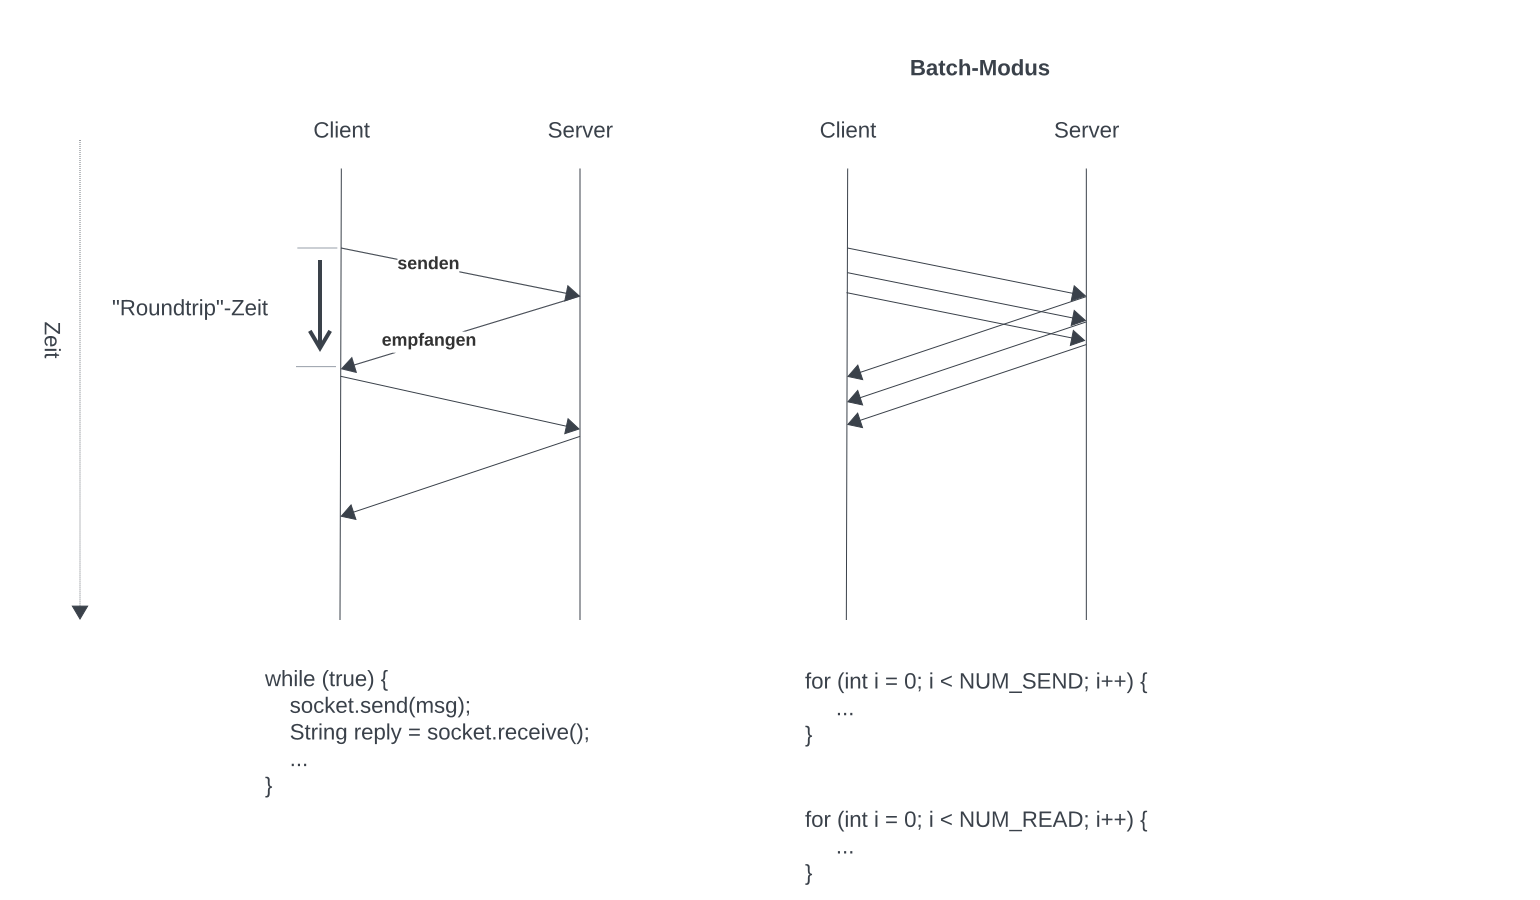
\includegraphics[scale=0.4]{chapters/Anhang/Klausuren/img/batchmodus}
    \caption{Vereinfachte Darstellung sequentieller Kommunikation und Batch-Modus (Quelle: eigene)}
    \label{fig:batchmodus}
\end{figure}
    
\begin{appendices}
    \input{chapters/Anhang/Zusatzaufgaben/index}
    \input{chapters/Anhang/Klausuren/ws13}
    \input{chapters/Anhang/Klausuren/ws15-16}
    \input{chapters/Anhang/Klausuren/ws16-17}
    \input{chapters/Anhang/Klausuren/ss19}
    \input{chapters/Anhang/Präsenzphase/index}

\end{appendices}


\end{appendices}


\end{appendices}



\begin{appendices}
    
\begin{appendices}
    
\begin{appendices}
    \input{chapters/Anhang/Zusatzaufgaben/index}
    \input{chapters/Anhang/Klausuren/ws13}
    \input{chapters/Anhang/Klausuren/ws15-16}
    \input{chapters/Anhang/Klausuren/ws16-17}
    \input{chapters/Anhang/Klausuren/ss19}
    \input{chapters/Anhang/Präsenzphase/index}

\end{appendices}

    \chapter{WS13}\label{ch:klausurws13}

\section{Aufgabe 1}
\subsection{Lösungsvorschlag}


\begin{minted}[mathescape,
    linenos,
    numbersep=5pt,
    gobble=2,
    fontsize=\small,
    frame=lines,
    framesep=2mm]{java}
    class Zahlenschloss {

        private int[] kombination;

        private int[] state;

        private boolean opened = false;

        public Zahlenschloss(int[] kombination) {
            this.kombination = kombination;
            this.state = new int[kombination.length];
        }

        public int anzahlRaedchen() {
            return kombination.length;
        }

        public synchronized int lesen(int radnummer) {
            return state[radnummer];
        }

        public synchronized void drehen(int radnummer, int zahl) {

            state[radnummer] = zahl;
            opened = true;
            for (int i = 0; i < anzahlRaedchen(); i++) {
                if (lesen(i) != kombination[i]) {
                    opened = false;
                    break;
                }
            }

            if (opened) {
                this.notify();
            }
        }

        public synchronized void warten() {

            while (!opened) {
                try {
                    this.wait();
                } catch (InterruptedException ignored) {}
            }
        }
    }
\end{minted}\\


\subsection{Anmerkung und Ergänzungen}

\begin{itemize}
    \item Es wird eine Wartebedingung benötigt, und zwar für die Methode \code{warten()}; ankommende Threads werden
    in die Warteschlange des Zahlenschloss-Objektes geschickt, wenn \code{opened} auf false gesetzt ist, ansonsten
    verlassen diese direkt die Methode wieder.\\
    Die Methode \code{drehen} benötigt keine separate Wartebedingung.
    Es reicht aus, sicherzustellen, dass das Zahlenschloss nicht gleichzeitig von anderen Threads benutzt werden kann:
    Die Methode \code{drehen} ist hierfür synchronisiert, damit das Zahlenschloss {insg.} immer nur eine Zustandsänderung
    erfährt - es sind andere Implementierungen möglich, in denen das Zahlenschloss dann von mehreren Threads gleichzeitig
    genutzt werden darf, wenn sich die Zugriffe anhand der ``Ziel``-\code{radnummer} unterscheiden, {bspw.} durch Mutex-Semaphore,
    die pro Radnummer verwendet werden\footnote{
        der gleichzeitige Zugriff auf unterschiedliche Arrays-Indizes ist erlaubt, s. `´17.4.1. Shared Variables``: \url{https://docs.oracle.com/javase/specs/jls/se21/html/jls-17.html#jls-1.4.1} - abgerufen 14.2.2024
    }.
    \item Es gibt nur eine Wartebedingung, von daher sollte \code{notify()} genügen.\\
    Wenn wir allerdings davon ausgehen, dass mehrere Threads über die Methode \code{warten()} in die Warteschlange des Objektes eingereiht worden sind,  sollte \code{notifyAll()} verwendet werden (siehe hierzu auch Abschnitt \ref{subsec:notifyAll}).
    Dennoch ist nicht garantiert, dass auch alle Threads aus der Warteschlange gelangen, denn es kann sein, dass ein anderer Thread die Methode \code{drehen()} betritt, dort die
    Zahlenkombination ändert und \code{opened} wieder auf \code{false} gesetzt wird. \\
    Ein anderer Thread, der nun in  \code{warten()} an die Reihe kommt, überprüft die Wartebedingung, und wird wieder in die Warteschlange eingereiht.
    Es ist also durchaus möglich, dass ein Thread nicht mehr aus der Methode \code{warten()} herauskommt.\\
    Dies könnte bspw. dadurch verhindert werden, dass die Threads in eine Queue gepackt werden, und in \code{drehen()} eine Wartebedingung eingefügt wird, die erst erfüllt ist,
    wenn die Queue geleert wurde oder aus ihr entnommen wurde, in der Reihenfolge, in der die Threads in die Queue eingereiht worden sind (\textit{FIFO}) (s. a. Abschnitt~\ref{subsec:readerwriterproblem}).
    \item Bei der Teilaufgabe mit der Schleife muss die komplette Schleife synchronisiert werden, was man durch ein \code{synchronized}-Statement erreicht\footnote{siehe Abschnitt~\ref{subsec:synchronizedstatement}.}
    \begin{minted}[mathescape,
        linenos,
        numbersep=5pt,
        gobble=2,
        fontsize=\small,
        frame=lines,
        framesep=2mm]{java}
        synchronized (zk) {
            for (int i = 0; i < anzahlRaedchen; i++) {
                System.out.println(zk.lesen(i));
            }
        }
    \end{minted}
    Ansonsten läuft man Gefahr, dass sich nach Auslesen der 1. Position der Wert von Position 2 geändert hat und dadurch eine
    Zahlenkombination ausgegeben wird, die es nicht gegeben hat:
    \begin{enumerate}
        \item $K\coloneqq[0, 0, 0]$
        \item Position $K_0$ wird ausgelesen und liefert $0$.
        \item Thread ändert $K_0$ zu $1$ $\implies K\coloneqq[1, 0, 0] $.
        \item Thread ändert $K_1$ zu $2$ $\implies K\coloneqq[1, 2, 0] $.
        \item Thread ändert $K_2$ zu $3$ $\implies K\coloneqq[1, 2, 3] $.
        \item Positionen $K_1$ und $K_2$ werden ausgelesen und liefern: $2, 3$
        \item Ausgabe: $0, 2, 3$ - diese Kombination hat es in dem Fall aber tatsächlich nicht gegeben.
    \end{enumerate}
\end{itemize}

\begin{tcolorbox}[colback=red!20,color=white,title=Anmerkung]
    Die Methode \code{lesen()} als \code{synchronized} zu markieren könnte man sich vlt. sparen, wenn man davon ausgeht,
    dass die Methode ohnehin in einem \code{synchronized}-Statement verwendet wird, um alle Rädchen abzulesen.\\
    Mehrere Threads können also nicht parallel auf unterschiedliche Positionen des Feldes zugreifen, wenn die Methode
    synchronisiert ist.\\
    Allerdings ist sowohl das Skript als auch das Buch recht klar, was in dieser Situation geschehen muss (s. Skript Fopt1/2, S. 9, außerdem \cite[31, Abschnitt 2.3.6]{Oec22}): Es muss (in diesem Kurs) immer \code{synchronized} verwendet werden, wenn gleichzeitig
    Daten geschrieben und gleichzeitig diese Daten gelesen werden sollen - und eine andere Implementierung, bei der die
    einzelnen Positionen ``gelocked`` sind, so dass ein gleichzeitiger Zugriff auf unterschiedliche Rädchen möglich ist, war nicht gefordert.\\
    Ggfl. würde in anderen Implementierungen der Einsatz von \code{AtomicReferenceArray}\footnote{s. \cite[157 ff.]{Oec22}
    s. ``Class AtomicReferenceArray<E>``: \url{https://docs.oracle.com/en/java/javase/21/docs/api/java.base/java/util/concurrent/atomic/AtomicReferenceArray.html} - abgerufen 15.2.2024
    } Sinn machen, aber das Lehrmaterial ist bereits sehr eindeutig bzgl. der Verwendung von \code{synchronized}.
\end{tcolorbox}



\section{Aufgabe 3}
\subsection{Lösungsvorschlag}

\subsection*{Statische Parallelität}
Statische Parallelität erlaubt es einem Server, eine \textit{fixe} Anzahl von Verbindungen gleichzeitig zu bedienen.\\
Hierbei wird ein Feld von Threads erstellt, wobei jeder Thread das \code{ServerSocket}-Objekt als Referenz übergeben bekommt.
In der \code{run()}-Methode wird dann über \code{accept()} in einer Endlosschleife auf eingehende Verbindungen gewartet, die dann so lange bedient werden, bis sich ein Client wieder abmeldet (oder eine andere Abbruchbedingung erfüllt ist, wie z.B. ein \code{SocketTimeout}).\\
Das sich ein Client abmeldet, bekommt man bspw. dadurch mit, dass \code{null} beim Lesen von einer Nachricht des Clients zurückgegeben wird (vgl. \cite[286]{Oec22}. \\
Siehe Abschnitt~\ref{sec:seqparserver} für ein Implementierungsbeispiel.



\subsection*{Dynamische Parallelität}

Bei der \textbf{Dynamischer Parallelität} erzeugt der Server für jede Verbindung einen neuen Thread, der so lange läuft, bis der Client die Verbindung wieder trennt.\\
Die Anzahl der Threads ändert sich dadurch laufend.\\
Wird die max. Anzahl erlaubter Threads nicht kontrolliert, kann es zu einer Überlastung des Server-Rechners kommen (bspw. durch einen Denial-of-Service-Angriff.)\\

\noindent
I.d.R. ist eine Mischform aus beidem geeignet, um mehrere Clients gleichzeitig bedienen zu können, und dabei nicht Gefahr zu laufen, durch dynamisches, unbegrenztes Wachstum der Anzahl der Threads überlastet zu werden.

    \chapter{WS13}\label{ch:klausurws5-16}

\section{Rechteck-Scroll (SS15 Aufgabe 2)}

Aufgabenstellung unklar.\\
Mögliche Implementierung unter \url{https://github.com/ThorstenSuckow/fopt/tree/main/src/main/java/klausurvorbereitung/foptws1516/MouseDragsSquareDemo}.

\section{Rechteck-Scroll (WS15/16 Aufgabe 1)}

Aufgabenstellung unklar.\\
Mögliche Implementierung unter \url{https://github.com/ThorstenSuckow/fopt/tree/main/src/main/java/klausurvorbereitung/foptws1516/MaxWeightDemo}.\\

\noindent
Es gibt nur eine Warteschlange für Threads in \code{use()}, es gibt keine Wartebedingung in \code{dontUse()} und damit auch keine weitere Warteschlange.\\
Es sind durch die Zugriffe auf unterschiedliche Indizes allerdings mehrere Wartebedingungen vorhanden, weshalb hab \code{notifyAll()} nutzen sollte,
sobald ein Zugriff auf ein Feld nach Aufruf von \code{dontUse} wieder möglich wird.\\
Ansonsten bestünde die Gefahr, dass bei dem Einsatz von \code{notify()} ein wartender Thread nicht geweckt wird, obwohl er weiterlaufen könnte:\\
Angenommen, das Feld $F$ hat eine Länge von $3$, das \code{maxWeight} ist mit $2$ konfiguriert.
Thread $t_1$ mit einer Laufzeit von $200\ sek$ bekommt Zugriff auf $F_0$, setzt $currentWeight$ auf $1$.\\
Thread $t_2$ mit einer Laufzeit von $1\ sek$ möchte auf $F_1$ zugreifen, setzt $currentWeight=2$ in die Warteschlange.\\
Thread $t_3$ meldet Zugriff auf $F_0$ an und gelangt in die Warteschlange.\\
Thread $t_4$ meldet Zugriff auf $F_1$ an und gelangt in die Warteschlange.\\
Thread $t_2$ ist mit der Bearbeitung von $F_1$ fertig, $currentWeight$ wird auf $1$ gesetzt, \code{notify()} wird aufgerufen.\\
Thread $t_3$ wird aus der Warteschlange geholt, kann aber nicht weiterarbeiten, da $F_0$ noch durch den länger dauernden $t_1$ blockiert ist, und kommt wieder in die Warteschlange.\\

\noindent
Offensichtlich hätte in dem Beispiel \code{notifyAll()} dazu geführt, dass auch $T_4$ seine Wartebedingung hätte überprüfen können, und hätte so Zugriff auf $F_1$ bekommen.
Stattdessen muss nun gewartet werden, bis das nächste \code{notify()} aufgerufen wird, oder ein neu ankommender Thread $F_1$ belegt.

    \chapter{WS16-17}\label{ch:klausurws16-17}

\section{Aufgabe 1}
\subsection{Lösungshinweis}

Die erste Aufgabe verdeutlicht, was bei einem \code{notifyAll()} und unsauber gesetzten Wartebedingungen passieren kann.\\
Sei folgender Quellcode gegeben:


\begin{minted}[mathescape,
    linenos,
    numbersep=5pt,
    gobble=2,
    fontsize=\small,
    frame=lines,
    framesep=2mm]{java}
    class Cond1AndCond2 {

        private boolean cond1;
        private boolean cond2;

        public synchronized void setCond1(boolean c) {
            cond1 = c;
            notifyAll();
        }

        public synchronized void setCond2(boolean c) {
            cond2 = c;
            notifyAll();
        }

        public synchronized void cond1AndCond2() {
            while(!cond1) {
                try {
                    wait();
                } catch(InterruptedException e) { }
            }

            while(!cond2) {
                try {
                    wait();
                } catch(InterruptedException e) {}
            }
            System.out.println("cond1 and cond2:" + cond1 + " " + cond2);
        }
    }
\end{minted}\\

Man sollte auf den ersten Blick meinen, dass \code{cond1} und \code{cond2} beide \code{true} sein müssen, damit die Ausgabe erfolgt.\\
Tatsächlich ist es aber so, dass es in der Methode zwei unterschiedliche Wartebedingungen gibt.\\
Die erste Wartebedingung schickt einen Thread in die Warteschlange, wenn \code{cond1 == false} gilt.\\
Setzt ein anderer Thread über \code{setCond1(true)} das Attribut entsprechend auf \code{true}, bewirkt der nachfolgende Aufruf von \code{notifyAll()}, dass alle \textit{wartenden} Threads aus der Warteschlange entfernt werden und erneut um eine Sperre des Objektes konkurrieren.\\
Erhält ein entsprechender Thread $t_w$ die Sperre auf das Objekt und kann seine \textit{while-wait-Schleife} verlassen, kann es vorkommen, dass er erneut in die Warteschlange eingereiht wird, wegen der nachfolgenden Wartebedingung \code{cond2 == false}.\\
Angenommen, ein weiterer Thread ruft nun \code{setCond2(true)} auf, und $t_w$ kommt aus der Warteschlange und konkurriert erneut und um die Sperre des Objektes, dann kann es vorkommen, das ein anderer Thread zunächst die Sperre erhält, \code{cond1} wieder auf \code{false} setzt, dann erhält $t_w$ die Sperre, überprüft die Wartebedingung \code{cond2 == false}.\\
Wegen \code{cond2} gelangt er aus der \textit{while-wait-Schleife} und die Ausgabe erfolgt - da zwischenzeitlich \code{cond1} wieder auf \code{false} gesetzt wurde, ist die erwartete Ausgabe nicht \code{true true}, sondern \code{false true} (s. Abbildung \ref{fig:cond1cond2}).\\

\begin{figure}
    \centering
    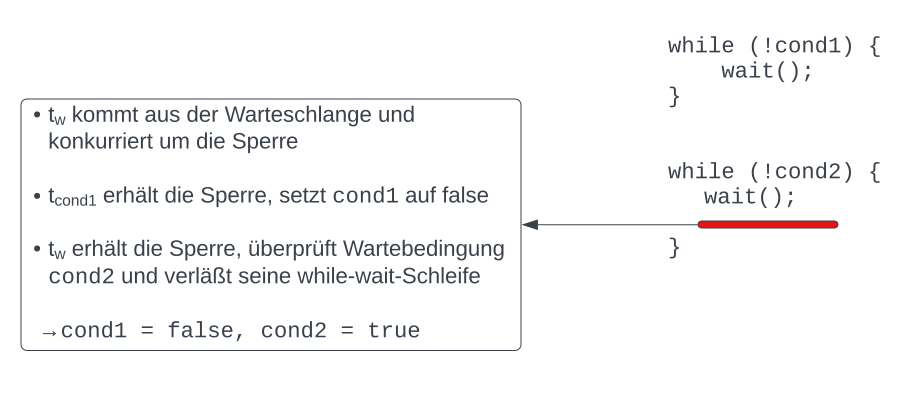
\includegraphics[scale=0.4]{chapters/Anhang/Klausuren/img/cond1cond2}
    \caption{in den rot markierten Bereich konkurriert $t_w$ um die Sperre des Objektes - wenn durch einen anderen Thread, der vor $t_w$ die Sperre erhält, \textit{cond1} auf \textit{false} gesetzt wird, stimmt die Ausgabe nicht mit der erwarteten überein. (Quelle: eigene)}
    \label{fig:cond1cond2}
\end{figure}

\noindent
Die korrekte Wartebedingung sollte lauten:

\begin{minted}[mathescape,
    linenos,
    numbersep=5pt,
    gobble=2,
    fontsize=\small,
    frame=lines,
    framesep=2mm]{java}
    public synchronized void cond1AndCond2() {
        while(!cond1 || !cond2) {
            try {
                wait();
            } catch(InterruptedException e) { }
        }
        System.out.println("cond1 and cond2:" + cond1 + " " + cond2);
    }
\end{minted}\\

Darüber hinaus müßte \code{notifyAll()} nur aufgerufen werden, wenn sowohl \code{cond1} als auch \code{cond2} auf \code{true} gesetzt sind, was leicht in den entsprechenden Methoden überprüft werden kann.
    \chapter{SS19}\label{ch:klausurss19}

\section{Aufgabe 1}

Bei der Aufgabe ist es wichtig, die Anforderungen genau zu beachten.\\
Ob eine Thread die while-wait-Schleife verlassen darf, wird von der Methode \code{tick()} gesteuert - wieviele Ticks ein Thread in der Schleife bleiben soll, wird von dem jeweiligen Thread definiert.\\
Die \code{tick()}-Methode wird von anderen Threads aufgerufen, es kann also durchaus vorkommen, dass mehrmals hintereinander
die \code{notifyAll()}-Methode aufgerufen wird - diese entfernt alle Threads aus der Warteschlange, damit die Threads ihre
Wartebedingungen erneut überprüfen können.\\
da \code{tick()} aber auch gleichzeitig einen Zähler realisieren soll, \textit{muss} es in der Methode auch eine Zählvariable geben, anhand derer die in der while-wait-Schleife enthaltenen Threads feststellen können, wie oft \code{tick()} aufgerufen wurde, um entsprechend aus der Schleife und nachfolgend der Methode herauszukommen.

\begin{figure}
    \centering
    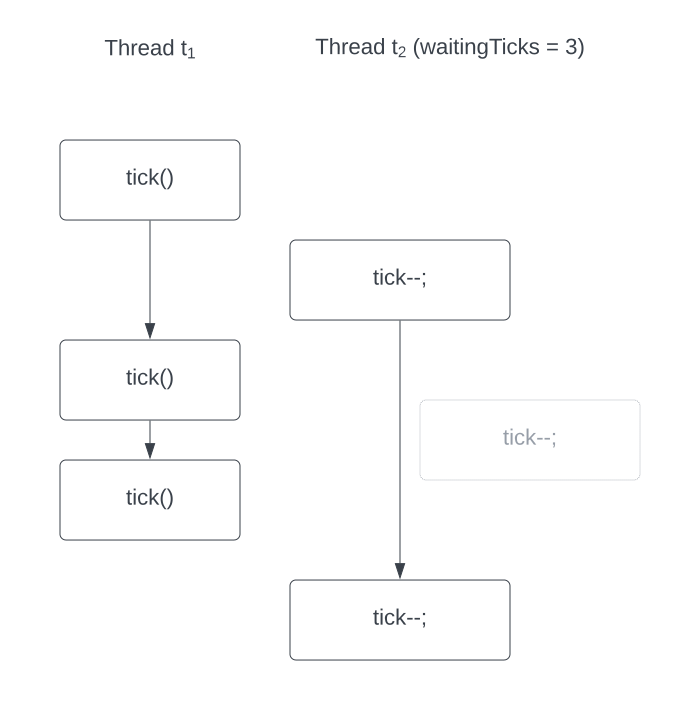
\includegraphics[scale=0.5]{chapters/Anhang/Klausuren/img/tick}
    \caption{Thread $t_1$ ruft 3 mal \texit{tick()} auf. Den Anforderungen nach müsste Thread $t_2$ danach aus der while-wait-Schleife herauskommen, erhält aber nicht die Sperre auf das Objekt von LogicalTime, um seinen eigenen Zähler rechtzeitig zu erniedrigen, bevor $t_1$ erneut \textit{tick()} aufruft. (Quelle: eigene)}
    \label{fig:tick}
\end{figure}

\section{Aufgabe 6}
Auch hier gilt, dass die Aufgabenstellung aufmerksam zu lesen ist.\\
Der Kreis soll erst ausgefüllt werden, wenn die Maustaste gelöst wird.

\begin{minted}[mathescape,
    linenos,
    numbersep=5pt,
    gobble=2,
    frame=lines,
    framesep=2mm]{java}
    private void mousePressed(double x, double y) {
        c = new Circle();
        c.setCenterX(x);
        c.setCenterY(y);
        c.setStroke(Color.RED);
        c.setFill(null); // oder Color.TRANSPARENT
        c.setRadius(RADIUS);
        graphicsPane.getChildren().add(c);
    }

    private void mouseReleased() {
        c.setFill(Color.RED);
        c = null;
    }
\end{minted}

\section{Aufgabe 8}

In der Abbildung \ref{fig:batchmodus} ist links der sequentielle Modus dargestellt, bei dem nach dem Senden einer Nachricht auf die Antwort des Servers gewartet wird, bevor eine neue Nachricht geschickt wird.
Dies wird i.d.R. verwendet, wenn das Senden einer neuen Nachricht abhängig ist von einem Ergebnis, die über die Server-Antwort übermittelt wird, oder wenn mit dem Server interagiert wird (Request abhängig vom Response).\\
Der Batch-Modus auf der rechten Seite der gleichen Abbildung ist schneller, da zwischen dem Senden von Nachrichten nicht auf Antworten gewartet werden müssen. \\
Erst nach dem Senden eine Batches von Nachrichten werden die dem Client zur Verfügung stehenden Antworten ausgelesen.\\

\noindent
In dieser Form des Batch-Modus besteht allerdings die Gefahr, dass es zu Verklemmungen kommt:
\begin{itemize}
    \item Bei dem Client kommen viele Nachrichten an, während er noch sendet.
    \item Die ankommenden Nachrichten für den Client werden gepuffert, bis sie ausgelesen werden (TCP- / OS-seitig).
    \item Läuft der Puffer voll, sorgt die Flusskontrolle (TCP) dafür, dass dem Sender mitgeteilt wird, dass keine Nachrichten mehr empfangen werden können, der Server sendet nicht mehr.
    \item Die zu sendenden Nachrichten des Servers werden in einen Puffer geschrieben.
    \item Der Sende-Puffer des Senders läuft voll.
    \item Bei dem nächsten Sende-Aufruf blockiert der Server, empfangene Nachrichten landen im Empfangspuffer
    \item Der Empfangspuffer des Servers läuft voll, der Client buffert die zu sendenden Nachrichten.
    \item Beide Anwendungen blockieren.
\end{itemize}

\\noindent
Um dieses Problem beim Batch-Modus zu umgehen, werden für das Senden und Empfangen zwei Threads auf Client-Seite erstellt: Ein Thread sendet, ein Thread empfängt. \\
Dadurch kann von dem Client immer wieder sein Empfangspuffer geleert werden, der Server wird beim Senden nicht blockiert.

\begin{figure}
    \centering
    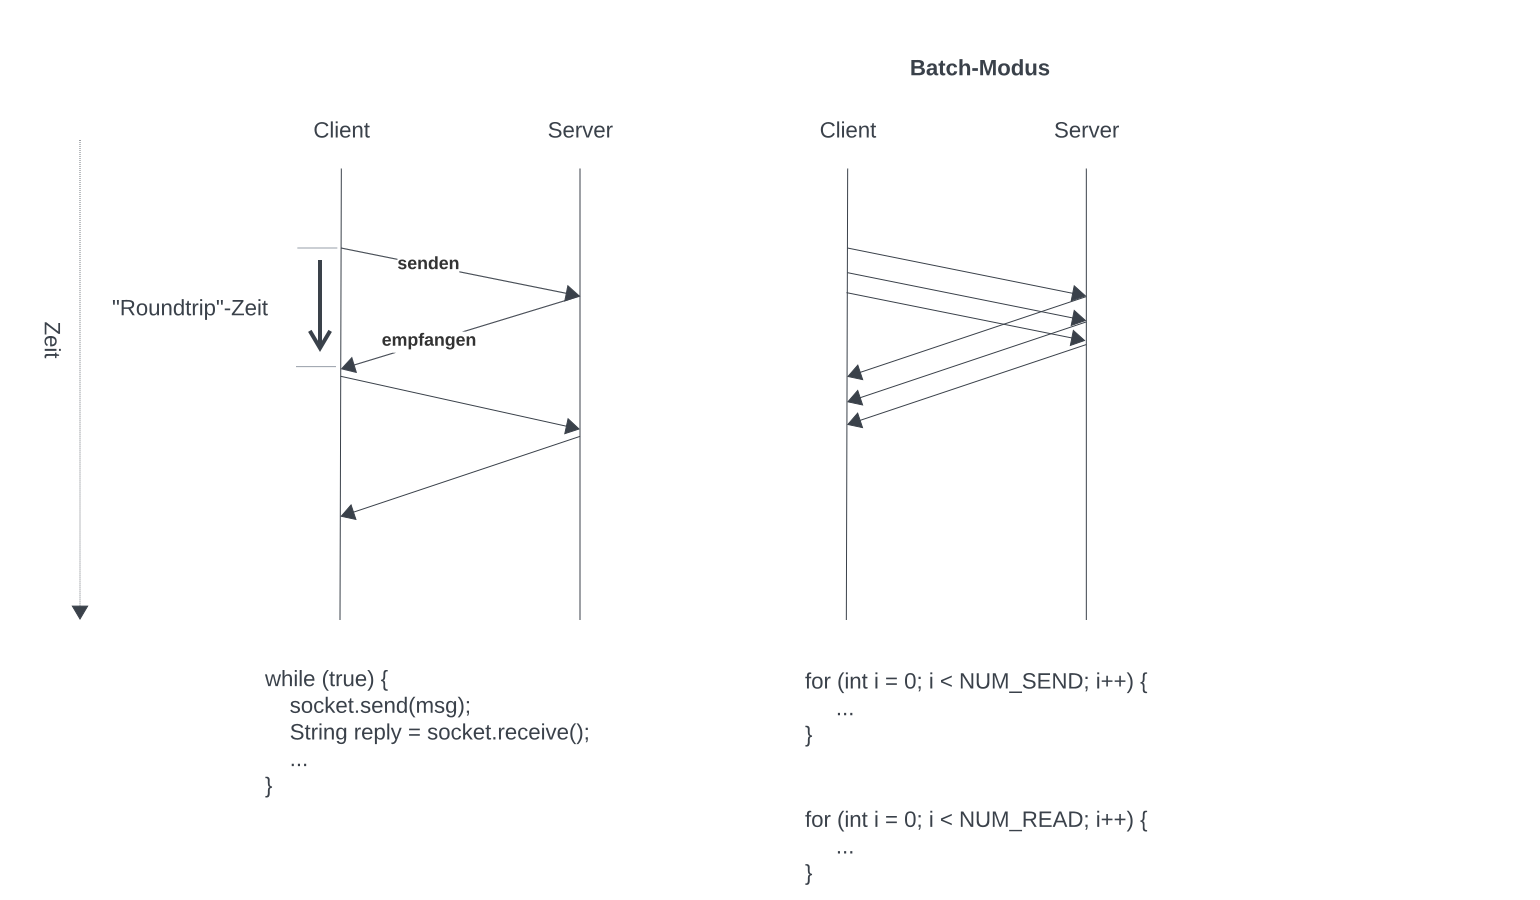
\includegraphics[scale=0.4]{chapters/Anhang/Klausuren/img/batchmodus}
    \caption{Vereinfachte Darstellung sequentieller Kommunikation und Batch-Modus (Quelle: eigene)}
    \label{fig:batchmodus}
\end{figure}
    
\begin{appendices}
    \input{chapters/Anhang/Zusatzaufgaben/index}
    \input{chapters/Anhang/Klausuren/ws13}
    \input{chapters/Anhang/Klausuren/ws15-16}
    \input{chapters/Anhang/Klausuren/ws16-17}
    \input{chapters/Anhang/Klausuren/ss19}
    \input{chapters/Anhang/Präsenzphase/index}

\end{appendices}


\end{appendices}

    \chapter{WS13}\label{ch:klausurws13}

\section{Aufgabe 1}
\subsection{Lösungsvorschlag}


\begin{minted}[mathescape,
    linenos,
    numbersep=5pt,
    gobble=2,
    fontsize=\small,
    frame=lines,
    framesep=2mm]{java}
    class Zahlenschloss {

        private int[] kombination;

        private int[] state;

        private boolean opened = false;

        public Zahlenschloss(int[] kombination) {
            this.kombination = kombination;
            this.state = new int[kombination.length];
        }

        public int anzahlRaedchen() {
            return kombination.length;
        }

        public synchronized int lesen(int radnummer) {
            return state[radnummer];
        }

        public synchronized void drehen(int radnummer, int zahl) {

            state[radnummer] = zahl;
            opened = true;
            for (int i = 0; i < anzahlRaedchen(); i++) {
                if (lesen(i) != kombination[i]) {
                    opened = false;
                    break;
                }
            }

            if (opened) {
                this.notify();
            }
        }

        public synchronized void warten() {

            while (!opened) {
                try {
                    this.wait();
                } catch (InterruptedException ignored) {}
            }
        }
    }
\end{minted}\\


\subsection{Anmerkung und Ergänzungen}

\begin{itemize}
    \item Es wird eine Wartebedingung benötigt, und zwar für die Methode \code{warten()}; ankommende Threads werden
    in die Warteschlange des Zahlenschloss-Objektes geschickt, wenn \code{opened} auf false gesetzt ist, ansonsten
    verlassen diese direkt die Methode wieder.\\
    Die Methode \code{drehen} benötigt keine separate Wartebedingung.
    Es reicht aus, sicherzustellen, dass das Zahlenschloss nicht gleichzeitig von anderen Threads benutzt werden kann:
    Die Methode \code{drehen} ist hierfür synchronisiert, damit das Zahlenschloss {insg.} immer nur eine Zustandsänderung
    erfährt - es sind andere Implementierungen möglich, in denen das Zahlenschloss dann von mehreren Threads gleichzeitig
    genutzt werden darf, wenn sich die Zugriffe anhand der ``Ziel``-\code{radnummer} unterscheiden, {bspw.} durch Mutex-Semaphore,
    die pro Radnummer verwendet werden\footnote{
        der gleichzeitige Zugriff auf unterschiedliche Arrays-Indizes ist erlaubt, s. `´17.4.1. Shared Variables``: \url{https://docs.oracle.com/javase/specs/jls/se21/html/jls-17.html#jls-1.4.1} - abgerufen 14.2.2024
    }.
    \item Es gibt nur eine Wartebedingung, von daher sollte \code{notify()} genügen.\\
    Wenn wir allerdings davon ausgehen, dass mehrere Threads über die Methode \code{warten()} in die Warteschlange des Objektes eingereiht worden sind,  sollte \code{notifyAll()} verwendet werden (siehe hierzu auch Abschnitt \ref{subsec:notifyAll}).
    Dennoch ist nicht garantiert, dass auch alle Threads aus der Warteschlange gelangen, denn es kann sein, dass ein anderer Thread die Methode \code{drehen()} betritt, dort die
    Zahlenkombination ändert und \code{opened} wieder auf \code{false} gesetzt wird. \\
    Ein anderer Thread, der nun in  \code{warten()} an die Reihe kommt, überprüft die Wartebedingung, und wird wieder in die Warteschlange eingereiht.
    Es ist also durchaus möglich, dass ein Thread nicht mehr aus der Methode \code{warten()} herauskommt.\\
    Dies könnte bspw. dadurch verhindert werden, dass die Threads in eine Queue gepackt werden, und in \code{drehen()} eine Wartebedingung eingefügt wird, die erst erfüllt ist,
    wenn die Queue geleert wurde oder aus ihr entnommen wurde, in der Reihenfolge, in der die Threads in die Queue eingereiht worden sind (\textit{FIFO}) (s. a. Abschnitt~\ref{subsec:readerwriterproblem}).
    \item Bei der Teilaufgabe mit der Schleife muss die komplette Schleife synchronisiert werden, was man durch ein \code{synchronized}-Statement erreicht\footnote{siehe Abschnitt~\ref{subsec:synchronizedstatement}.}
    \begin{minted}[mathescape,
        linenos,
        numbersep=5pt,
        gobble=2,
        fontsize=\small,
        frame=lines,
        framesep=2mm]{java}
        synchronized (zk) {
            for (int i = 0; i < anzahlRaedchen; i++) {
                System.out.println(zk.lesen(i));
            }
        }
    \end{minted}
    Ansonsten läuft man Gefahr, dass sich nach Auslesen der 1. Position der Wert von Position 2 geändert hat und dadurch eine
    Zahlenkombination ausgegeben wird, die es nicht gegeben hat:
    \begin{enumerate}
        \item $K\coloneqq[0, 0, 0]$
        \item Position $K_0$ wird ausgelesen und liefert $0$.
        \item Thread ändert $K_0$ zu $1$ $\implies K\coloneqq[1, 0, 0] $.
        \item Thread ändert $K_1$ zu $2$ $\implies K\coloneqq[1, 2, 0] $.
        \item Thread ändert $K_2$ zu $3$ $\implies K\coloneqq[1, 2, 3] $.
        \item Positionen $K_1$ und $K_2$ werden ausgelesen und liefern: $2, 3$
        \item Ausgabe: $0, 2, 3$ - diese Kombination hat es in dem Fall aber tatsächlich nicht gegeben.
    \end{enumerate}
\end{itemize}

\begin{tcolorbox}[colback=red!20,color=white,title=Anmerkung]
    Die Methode \code{lesen()} als \code{synchronized} zu markieren könnte man sich vlt. sparen, wenn man davon ausgeht,
    dass die Methode ohnehin in einem \code{synchronized}-Statement verwendet wird, um alle Rädchen abzulesen.\\
    Mehrere Threads können also nicht parallel auf unterschiedliche Positionen des Feldes zugreifen, wenn die Methode
    synchronisiert ist.\\
    Allerdings ist sowohl das Skript als auch das Buch recht klar, was in dieser Situation geschehen muss (s. Skript Fopt1/2, S. 9, außerdem \cite[31, Abschnitt 2.3.6]{Oec22}): Es muss (in diesem Kurs) immer \code{synchronized} verwendet werden, wenn gleichzeitig
    Daten geschrieben und gleichzeitig diese Daten gelesen werden sollen - und eine andere Implementierung, bei der die
    einzelnen Positionen ``gelocked`` sind, so dass ein gleichzeitiger Zugriff auf unterschiedliche Rädchen möglich ist, war nicht gefordert.\\
    Ggfl. würde in anderen Implementierungen der Einsatz von \code{AtomicReferenceArray}\footnote{s. \cite[157 ff.]{Oec22}
    s. ``Class AtomicReferenceArray<E>``: \url{https://docs.oracle.com/en/java/javase/21/docs/api/java.base/java/util/concurrent/atomic/AtomicReferenceArray.html} - abgerufen 15.2.2024
    } Sinn machen, aber das Lehrmaterial ist bereits sehr eindeutig bzgl. der Verwendung von \code{synchronized}.
\end{tcolorbox}



\section{Aufgabe 3}
\subsection{Lösungsvorschlag}

\subsection*{Statische Parallelität}
Statische Parallelität erlaubt es einem Server, eine \textit{fixe} Anzahl von Verbindungen gleichzeitig zu bedienen.\\
Hierbei wird ein Feld von Threads erstellt, wobei jeder Thread das \code{ServerSocket}-Objekt als Referenz übergeben bekommt.
In der \code{run()}-Methode wird dann über \code{accept()} in einer Endlosschleife auf eingehende Verbindungen gewartet, die dann so lange bedient werden, bis sich ein Client wieder abmeldet (oder eine andere Abbruchbedingung erfüllt ist, wie z.B. ein \code{SocketTimeout}).\\
Das sich ein Client abmeldet, bekommt man bspw. dadurch mit, dass \code{null} beim Lesen von einer Nachricht des Clients zurückgegeben wird (vgl. \cite[286]{Oec22}. \\
Siehe Abschnitt~\ref{sec:seqparserver} für ein Implementierungsbeispiel.



\subsection*{Dynamische Parallelität}

Bei der \textbf{Dynamischer Parallelität} erzeugt der Server für jede Verbindung einen neuen Thread, der so lange läuft, bis der Client die Verbindung wieder trennt.\\
Die Anzahl der Threads ändert sich dadurch laufend.\\
Wird die max. Anzahl erlaubter Threads nicht kontrolliert, kann es zu einer Überlastung des Server-Rechners kommen (bspw. durch einen Denial-of-Service-Angriff.)\\

\noindent
I.d.R. ist eine Mischform aus beidem geeignet, um mehrere Clients gleichzeitig bedienen zu können, und dabei nicht Gefahr zu laufen, durch dynamisches, unbegrenztes Wachstum der Anzahl der Threads überlastet zu werden.

    \chapter{WS13}\label{ch:klausurws5-16}

\section{Rechteck-Scroll (SS15 Aufgabe 2)}

Aufgabenstellung unklar.\\
Mögliche Implementierung unter \url{https://github.com/ThorstenSuckow/fopt/tree/main/src/main/java/klausurvorbereitung/foptws1516/MouseDragsSquareDemo}.

\section{Rechteck-Scroll (WS15/16 Aufgabe 1)}

Aufgabenstellung unklar.\\
Mögliche Implementierung unter \url{https://github.com/ThorstenSuckow/fopt/tree/main/src/main/java/klausurvorbereitung/foptws1516/MaxWeightDemo}.\\

\noindent
Es gibt nur eine Warteschlange für Threads in \code{use()}, es gibt keine Wartebedingung in \code{dontUse()} und damit auch keine weitere Warteschlange.\\
Es sind durch die Zugriffe auf unterschiedliche Indizes allerdings mehrere Wartebedingungen vorhanden, weshalb hab \code{notifyAll()} nutzen sollte,
sobald ein Zugriff auf ein Feld nach Aufruf von \code{dontUse} wieder möglich wird.\\
Ansonsten bestünde die Gefahr, dass bei dem Einsatz von \code{notify()} ein wartender Thread nicht geweckt wird, obwohl er weiterlaufen könnte:\\
Angenommen, das Feld $F$ hat eine Länge von $3$, das \code{maxWeight} ist mit $2$ konfiguriert.
Thread $t_1$ mit einer Laufzeit von $200\ sek$ bekommt Zugriff auf $F_0$, setzt $currentWeight$ auf $1$.\\
Thread $t_2$ mit einer Laufzeit von $1\ sek$ möchte auf $F_1$ zugreifen, setzt $currentWeight=2$ in die Warteschlange.\\
Thread $t_3$ meldet Zugriff auf $F_0$ an und gelangt in die Warteschlange.\\
Thread $t_4$ meldet Zugriff auf $F_1$ an und gelangt in die Warteschlange.\\
Thread $t_2$ ist mit der Bearbeitung von $F_1$ fertig, $currentWeight$ wird auf $1$ gesetzt, \code{notify()} wird aufgerufen.\\
Thread $t_3$ wird aus der Warteschlange geholt, kann aber nicht weiterarbeiten, da $F_0$ noch durch den länger dauernden $t_1$ blockiert ist, und kommt wieder in die Warteschlange.\\

\noindent
Offensichtlich hätte in dem Beispiel \code{notifyAll()} dazu geführt, dass auch $T_4$ seine Wartebedingung hätte überprüfen können, und hätte so Zugriff auf $F_1$ bekommen.
Stattdessen muss nun gewartet werden, bis das nächste \code{notify()} aufgerufen wird, oder ein neu ankommender Thread $F_1$ belegt.

    \chapter{WS16-17}\label{ch:klausurws16-17}

\section{Aufgabe 1}
\subsection{Lösungshinweis}

Die erste Aufgabe verdeutlicht, was bei einem \code{notifyAll()} und unsauber gesetzten Wartebedingungen passieren kann.\\
Sei folgender Quellcode gegeben:


\begin{minted}[mathescape,
    linenos,
    numbersep=5pt,
    gobble=2,
    fontsize=\small,
    frame=lines,
    framesep=2mm]{java}
    class Cond1AndCond2 {

        private boolean cond1;
        private boolean cond2;

        public synchronized void setCond1(boolean c) {
            cond1 = c;
            notifyAll();
        }

        public synchronized void setCond2(boolean c) {
            cond2 = c;
            notifyAll();
        }

        public synchronized void cond1AndCond2() {
            while(!cond1) {
                try {
                    wait();
                } catch(InterruptedException e) { }
            }

            while(!cond2) {
                try {
                    wait();
                } catch(InterruptedException e) {}
            }
            System.out.println("cond1 and cond2:" + cond1 + " " + cond2);
        }
    }
\end{minted}\\

Man sollte auf den ersten Blick meinen, dass \code{cond1} und \code{cond2} beide \code{true} sein müssen, damit die Ausgabe erfolgt.\\
Tatsächlich ist es aber so, dass es in der Methode zwei unterschiedliche Wartebedingungen gibt.\\
Die erste Wartebedingung schickt einen Thread in die Warteschlange, wenn \code{cond1 == false} gilt.\\
Setzt ein anderer Thread über \code{setCond1(true)} das Attribut entsprechend auf \code{true}, bewirkt der nachfolgende Aufruf von \code{notifyAll()}, dass alle \textit{wartenden} Threads aus der Warteschlange entfernt werden und erneut um eine Sperre des Objektes konkurrieren.\\
Erhält ein entsprechender Thread $t_w$ die Sperre auf das Objekt und kann seine \textit{while-wait-Schleife} verlassen, kann es vorkommen, dass er erneut in die Warteschlange eingereiht wird, wegen der nachfolgenden Wartebedingung \code{cond2 == false}.\\
Angenommen, ein weiterer Thread ruft nun \code{setCond2(true)} auf, und $t_w$ kommt aus der Warteschlange und konkurriert erneut und um die Sperre des Objektes, dann kann es vorkommen, das ein anderer Thread zunächst die Sperre erhält, \code{cond1} wieder auf \code{false} setzt, dann erhält $t_w$ die Sperre, überprüft die Wartebedingung \code{cond2 == false}.\\
Wegen \code{cond2} gelangt er aus der \textit{while-wait-Schleife} und die Ausgabe erfolgt - da zwischenzeitlich \code{cond1} wieder auf \code{false} gesetzt wurde, ist die erwartete Ausgabe nicht \code{true true}, sondern \code{false true} (s. Abbildung \ref{fig:cond1cond2}).\\

\begin{figure}
    \centering
    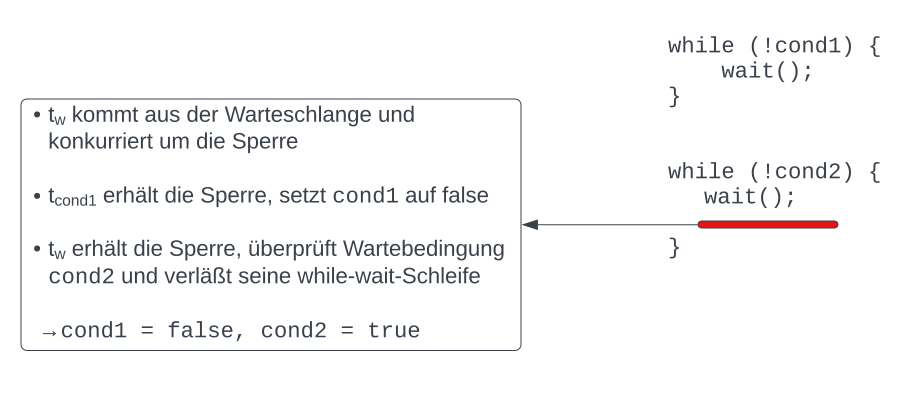
\includegraphics[scale=0.4]{chapters/Anhang/Klausuren/img/cond1cond2}
    \caption{in den rot markierten Bereich konkurriert $t_w$ um die Sperre des Objektes - wenn durch einen anderen Thread, der vor $t_w$ die Sperre erhält, \textit{cond1} auf \textit{false} gesetzt wird, stimmt die Ausgabe nicht mit der erwarteten überein. (Quelle: eigene)}
    \label{fig:cond1cond2}
\end{figure}

\noindent
Die korrekte Wartebedingung sollte lauten:

\begin{minted}[mathescape,
    linenos,
    numbersep=5pt,
    gobble=2,
    fontsize=\small,
    frame=lines,
    framesep=2mm]{java}
    public synchronized void cond1AndCond2() {
        while(!cond1 || !cond2) {
            try {
                wait();
            } catch(InterruptedException e) { }
        }
        System.out.println("cond1 and cond2:" + cond1 + " " + cond2);
    }
\end{minted}\\

Darüber hinaus müßte \code{notifyAll()} nur aufgerufen werden, wenn sowohl \code{cond1} als auch \code{cond2} auf \code{true} gesetzt sind, was leicht in den entsprechenden Methoden überprüft werden kann.
    \chapter{SS19}\label{ch:klausurss19}

\section{Aufgabe 1}

Bei der Aufgabe ist es wichtig, die Anforderungen genau zu beachten.\\
Ob eine Thread die while-wait-Schleife verlassen darf, wird von der Methode \code{tick()} gesteuert - wieviele Ticks ein Thread in der Schleife bleiben soll, wird von dem jeweiligen Thread definiert.\\
Die \code{tick()}-Methode wird von anderen Threads aufgerufen, es kann also durchaus vorkommen, dass mehrmals hintereinander
die \code{notifyAll()}-Methode aufgerufen wird - diese entfernt alle Threads aus der Warteschlange, damit die Threads ihre
Wartebedingungen erneut überprüfen können.\\
da \code{tick()} aber auch gleichzeitig einen Zähler realisieren soll, \textit{muss} es in der Methode auch eine Zählvariable geben, anhand derer die in der while-wait-Schleife enthaltenen Threads feststellen können, wie oft \code{tick()} aufgerufen wurde, um entsprechend aus der Schleife und nachfolgend der Methode herauszukommen.

\begin{figure}
    \centering
    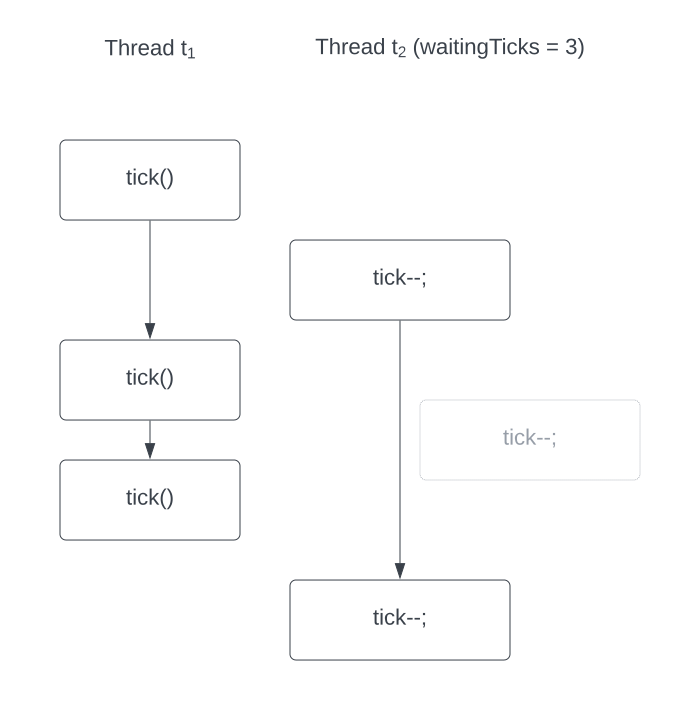
\includegraphics[scale=0.5]{chapters/Anhang/Klausuren/img/tick}
    \caption{Thread $t_1$ ruft 3 mal \texit{tick()} auf. Den Anforderungen nach müsste Thread $t_2$ danach aus der while-wait-Schleife herauskommen, erhält aber nicht die Sperre auf das Objekt von LogicalTime, um seinen eigenen Zähler rechtzeitig zu erniedrigen, bevor $t_1$ erneut \textit{tick()} aufruft. (Quelle: eigene)}
    \label{fig:tick}
\end{figure}

\section{Aufgabe 6}
Auch hier gilt, dass die Aufgabenstellung aufmerksam zu lesen ist.\\
Der Kreis soll erst ausgefüllt werden, wenn die Maustaste gelöst wird.

\begin{minted}[mathescape,
    linenos,
    numbersep=5pt,
    gobble=2,
    frame=lines,
    framesep=2mm]{java}
    private void mousePressed(double x, double y) {
        c = new Circle();
        c.setCenterX(x);
        c.setCenterY(y);
        c.setStroke(Color.RED);
        c.setFill(null); // oder Color.TRANSPARENT
        c.setRadius(RADIUS);
        graphicsPane.getChildren().add(c);
    }

    private void mouseReleased() {
        c.setFill(Color.RED);
        c = null;
    }
\end{minted}

\section{Aufgabe 8}

In der Abbildung \ref{fig:batchmodus} ist links der sequentielle Modus dargestellt, bei dem nach dem Senden einer Nachricht auf die Antwort des Servers gewartet wird, bevor eine neue Nachricht geschickt wird.
Dies wird i.d.R. verwendet, wenn das Senden einer neuen Nachricht abhängig ist von einem Ergebnis, die über die Server-Antwort übermittelt wird, oder wenn mit dem Server interagiert wird (Request abhängig vom Response).\\
Der Batch-Modus auf der rechten Seite der gleichen Abbildung ist schneller, da zwischen dem Senden von Nachrichten nicht auf Antworten gewartet werden müssen. \\
Erst nach dem Senden eine Batches von Nachrichten werden die dem Client zur Verfügung stehenden Antworten ausgelesen.\\

\noindent
In dieser Form des Batch-Modus besteht allerdings die Gefahr, dass es zu Verklemmungen kommt:
\begin{itemize}
    \item Bei dem Client kommen viele Nachrichten an, während er noch sendet.
    \item Die ankommenden Nachrichten für den Client werden gepuffert, bis sie ausgelesen werden (TCP- / OS-seitig).
    \item Läuft der Puffer voll, sorgt die Flusskontrolle (TCP) dafür, dass dem Sender mitgeteilt wird, dass keine Nachrichten mehr empfangen werden können, der Server sendet nicht mehr.
    \item Die zu sendenden Nachrichten des Servers werden in einen Puffer geschrieben.
    \item Der Sende-Puffer des Senders läuft voll.
    \item Bei dem nächsten Sende-Aufruf blockiert der Server, empfangene Nachrichten landen im Empfangspuffer
    \item Der Empfangspuffer des Servers läuft voll, der Client buffert die zu sendenden Nachrichten.
    \item Beide Anwendungen blockieren.
\end{itemize}

\\noindent
Um dieses Problem beim Batch-Modus zu umgehen, werden für das Senden und Empfangen zwei Threads auf Client-Seite erstellt: Ein Thread sendet, ein Thread empfängt. \\
Dadurch kann von dem Client immer wieder sein Empfangspuffer geleert werden, der Server wird beim Senden nicht blockiert.

\begin{figure}
    \centering
    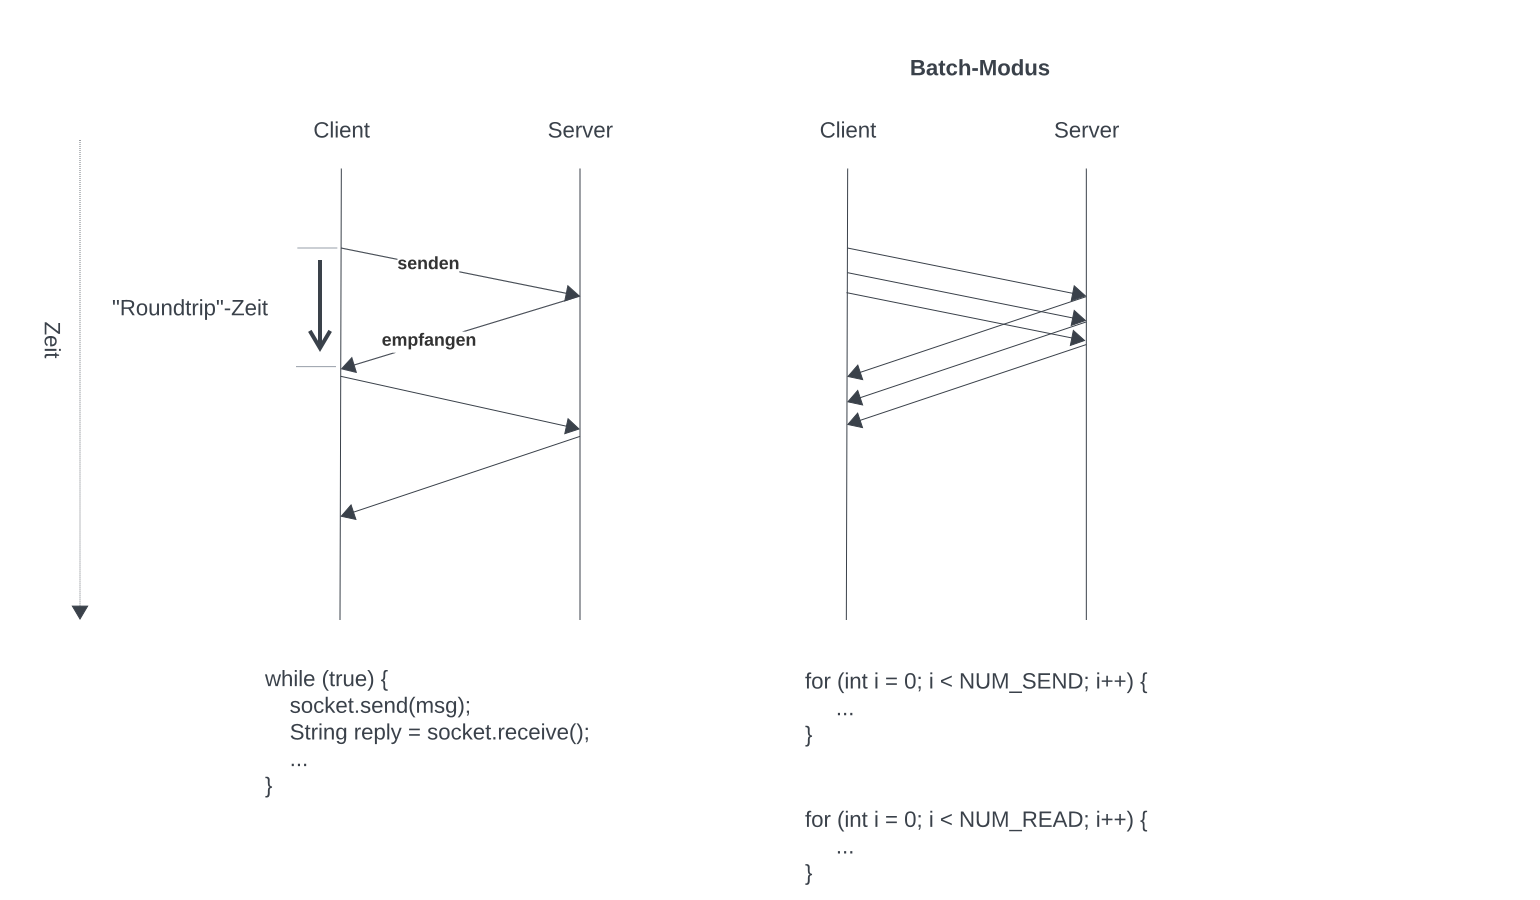
\includegraphics[scale=0.4]{chapters/Anhang/Klausuren/img/batchmodus}
    \caption{Vereinfachte Darstellung sequentieller Kommunikation und Batch-Modus (Quelle: eigene)}
    \label{fig:batchmodus}
\end{figure}
    
\begin{appendices}
    
\begin{appendices}
    \input{chapters/Anhang/Zusatzaufgaben/index}
    \input{chapters/Anhang/Klausuren/ws13}
    \input{chapters/Anhang/Klausuren/ws15-16}
    \input{chapters/Anhang/Klausuren/ws16-17}
    \input{chapters/Anhang/Klausuren/ss19}
    \input{chapters/Anhang/Präsenzphase/index}

\end{appendices}

    \chapter{WS13}\label{ch:klausurws13}

\section{Aufgabe 1}
\subsection{Lösungsvorschlag}


\begin{minted}[mathescape,
    linenos,
    numbersep=5pt,
    gobble=2,
    fontsize=\small,
    frame=lines,
    framesep=2mm]{java}
    class Zahlenschloss {

        private int[] kombination;

        private int[] state;

        private boolean opened = false;

        public Zahlenschloss(int[] kombination) {
            this.kombination = kombination;
            this.state = new int[kombination.length];
        }

        public int anzahlRaedchen() {
            return kombination.length;
        }

        public synchronized int lesen(int radnummer) {
            return state[radnummer];
        }

        public synchronized void drehen(int radnummer, int zahl) {

            state[radnummer] = zahl;
            opened = true;
            for (int i = 0; i < anzahlRaedchen(); i++) {
                if (lesen(i) != kombination[i]) {
                    opened = false;
                    break;
                }
            }

            if (opened) {
                this.notify();
            }
        }

        public synchronized void warten() {

            while (!opened) {
                try {
                    this.wait();
                } catch (InterruptedException ignored) {}
            }
        }
    }
\end{minted}\\


\subsection{Anmerkung und Ergänzungen}

\begin{itemize}
    \item Es wird eine Wartebedingung benötigt, und zwar für die Methode \code{warten()}; ankommende Threads werden
    in die Warteschlange des Zahlenschloss-Objektes geschickt, wenn \code{opened} auf false gesetzt ist, ansonsten
    verlassen diese direkt die Methode wieder.\\
    Die Methode \code{drehen} benötigt keine separate Wartebedingung.
    Es reicht aus, sicherzustellen, dass das Zahlenschloss nicht gleichzeitig von anderen Threads benutzt werden kann:
    Die Methode \code{drehen} ist hierfür synchronisiert, damit das Zahlenschloss {insg.} immer nur eine Zustandsänderung
    erfährt - es sind andere Implementierungen möglich, in denen das Zahlenschloss dann von mehreren Threads gleichzeitig
    genutzt werden darf, wenn sich die Zugriffe anhand der ``Ziel``-\code{radnummer} unterscheiden, {bspw.} durch Mutex-Semaphore,
    die pro Radnummer verwendet werden\footnote{
        der gleichzeitige Zugriff auf unterschiedliche Arrays-Indizes ist erlaubt, s. `´17.4.1. Shared Variables``: \url{https://docs.oracle.com/javase/specs/jls/se21/html/jls-17.html#jls-1.4.1} - abgerufen 14.2.2024
    }.
    \item Es gibt nur eine Wartebedingung, von daher sollte \code{notify()} genügen.\\
    Wenn wir allerdings davon ausgehen, dass mehrere Threads über die Methode \code{warten()} in die Warteschlange des Objektes eingereiht worden sind,  sollte \code{notifyAll()} verwendet werden (siehe hierzu auch Abschnitt \ref{subsec:notifyAll}).
    Dennoch ist nicht garantiert, dass auch alle Threads aus der Warteschlange gelangen, denn es kann sein, dass ein anderer Thread die Methode \code{drehen()} betritt, dort die
    Zahlenkombination ändert und \code{opened} wieder auf \code{false} gesetzt wird. \\
    Ein anderer Thread, der nun in  \code{warten()} an die Reihe kommt, überprüft die Wartebedingung, und wird wieder in die Warteschlange eingereiht.
    Es ist also durchaus möglich, dass ein Thread nicht mehr aus der Methode \code{warten()} herauskommt.\\
    Dies könnte bspw. dadurch verhindert werden, dass die Threads in eine Queue gepackt werden, und in \code{drehen()} eine Wartebedingung eingefügt wird, die erst erfüllt ist,
    wenn die Queue geleert wurde oder aus ihr entnommen wurde, in der Reihenfolge, in der die Threads in die Queue eingereiht worden sind (\textit{FIFO}) (s. a. Abschnitt~\ref{subsec:readerwriterproblem}).
    \item Bei der Teilaufgabe mit der Schleife muss die komplette Schleife synchronisiert werden, was man durch ein \code{synchronized}-Statement erreicht\footnote{siehe Abschnitt~\ref{subsec:synchronizedstatement}.}
    \begin{minted}[mathescape,
        linenos,
        numbersep=5pt,
        gobble=2,
        fontsize=\small,
        frame=lines,
        framesep=2mm]{java}
        synchronized (zk) {
            for (int i = 0; i < anzahlRaedchen; i++) {
                System.out.println(zk.lesen(i));
            }
        }
    \end{minted}
    Ansonsten läuft man Gefahr, dass sich nach Auslesen der 1. Position der Wert von Position 2 geändert hat und dadurch eine
    Zahlenkombination ausgegeben wird, die es nicht gegeben hat:
    \begin{enumerate}
        \item $K\coloneqq[0, 0, 0]$
        \item Position $K_0$ wird ausgelesen und liefert $0$.
        \item Thread ändert $K_0$ zu $1$ $\implies K\coloneqq[1, 0, 0] $.
        \item Thread ändert $K_1$ zu $2$ $\implies K\coloneqq[1, 2, 0] $.
        \item Thread ändert $K_2$ zu $3$ $\implies K\coloneqq[1, 2, 3] $.
        \item Positionen $K_1$ und $K_2$ werden ausgelesen und liefern: $2, 3$
        \item Ausgabe: $0, 2, 3$ - diese Kombination hat es in dem Fall aber tatsächlich nicht gegeben.
    \end{enumerate}
\end{itemize}

\begin{tcolorbox}[colback=red!20,color=white,title=Anmerkung]
    Die Methode \code{lesen()} als \code{synchronized} zu markieren könnte man sich vlt. sparen, wenn man davon ausgeht,
    dass die Methode ohnehin in einem \code{synchronized}-Statement verwendet wird, um alle Rädchen abzulesen.\\
    Mehrere Threads können also nicht parallel auf unterschiedliche Positionen des Feldes zugreifen, wenn die Methode
    synchronisiert ist.\\
    Allerdings ist sowohl das Skript als auch das Buch recht klar, was in dieser Situation geschehen muss (s. Skript Fopt1/2, S. 9, außerdem \cite[31, Abschnitt 2.3.6]{Oec22}): Es muss (in diesem Kurs) immer \code{synchronized} verwendet werden, wenn gleichzeitig
    Daten geschrieben und gleichzeitig diese Daten gelesen werden sollen - und eine andere Implementierung, bei der die
    einzelnen Positionen ``gelocked`` sind, so dass ein gleichzeitiger Zugriff auf unterschiedliche Rädchen möglich ist, war nicht gefordert.\\
    Ggfl. würde in anderen Implementierungen der Einsatz von \code{AtomicReferenceArray}\footnote{s. \cite[157 ff.]{Oec22}
    s. ``Class AtomicReferenceArray<E>``: \url{https://docs.oracle.com/en/java/javase/21/docs/api/java.base/java/util/concurrent/atomic/AtomicReferenceArray.html} - abgerufen 15.2.2024
    } Sinn machen, aber das Lehrmaterial ist bereits sehr eindeutig bzgl. der Verwendung von \code{synchronized}.
\end{tcolorbox}



\section{Aufgabe 3}
\subsection{Lösungsvorschlag}

\subsection*{Statische Parallelität}
Statische Parallelität erlaubt es einem Server, eine \textit{fixe} Anzahl von Verbindungen gleichzeitig zu bedienen.\\
Hierbei wird ein Feld von Threads erstellt, wobei jeder Thread das \code{ServerSocket}-Objekt als Referenz übergeben bekommt.
In der \code{run()}-Methode wird dann über \code{accept()} in einer Endlosschleife auf eingehende Verbindungen gewartet, die dann so lange bedient werden, bis sich ein Client wieder abmeldet (oder eine andere Abbruchbedingung erfüllt ist, wie z.B. ein \code{SocketTimeout}).\\
Das sich ein Client abmeldet, bekommt man bspw. dadurch mit, dass \code{null} beim Lesen von einer Nachricht des Clients zurückgegeben wird (vgl. \cite[286]{Oec22}. \\
Siehe Abschnitt~\ref{sec:seqparserver} für ein Implementierungsbeispiel.



\subsection*{Dynamische Parallelität}

Bei der \textbf{Dynamischer Parallelität} erzeugt der Server für jede Verbindung einen neuen Thread, der so lange läuft, bis der Client die Verbindung wieder trennt.\\
Die Anzahl der Threads ändert sich dadurch laufend.\\
Wird die max. Anzahl erlaubter Threads nicht kontrolliert, kann es zu einer Überlastung des Server-Rechners kommen (bspw. durch einen Denial-of-Service-Angriff.)\\

\noindent
I.d.R. ist eine Mischform aus beidem geeignet, um mehrere Clients gleichzeitig bedienen zu können, und dabei nicht Gefahr zu laufen, durch dynamisches, unbegrenztes Wachstum der Anzahl der Threads überlastet zu werden.

    \chapter{WS13}\label{ch:klausurws5-16}

\section{Rechteck-Scroll (SS15 Aufgabe 2)}

Aufgabenstellung unklar.\\
Mögliche Implementierung unter \url{https://github.com/ThorstenSuckow/fopt/tree/main/src/main/java/klausurvorbereitung/foptws1516/MouseDragsSquareDemo}.

\section{Rechteck-Scroll (WS15/16 Aufgabe 1)}

Aufgabenstellung unklar.\\
Mögliche Implementierung unter \url{https://github.com/ThorstenSuckow/fopt/tree/main/src/main/java/klausurvorbereitung/foptws1516/MaxWeightDemo}.\\

\noindent
Es gibt nur eine Warteschlange für Threads in \code{use()}, es gibt keine Wartebedingung in \code{dontUse()} und damit auch keine weitere Warteschlange.\\
Es sind durch die Zugriffe auf unterschiedliche Indizes allerdings mehrere Wartebedingungen vorhanden, weshalb hab \code{notifyAll()} nutzen sollte,
sobald ein Zugriff auf ein Feld nach Aufruf von \code{dontUse} wieder möglich wird.\\
Ansonsten bestünde die Gefahr, dass bei dem Einsatz von \code{notify()} ein wartender Thread nicht geweckt wird, obwohl er weiterlaufen könnte:\\
Angenommen, das Feld $F$ hat eine Länge von $3$, das \code{maxWeight} ist mit $2$ konfiguriert.
Thread $t_1$ mit einer Laufzeit von $200\ sek$ bekommt Zugriff auf $F_0$, setzt $currentWeight$ auf $1$.\\
Thread $t_2$ mit einer Laufzeit von $1\ sek$ möchte auf $F_1$ zugreifen, setzt $currentWeight=2$ in die Warteschlange.\\
Thread $t_3$ meldet Zugriff auf $F_0$ an und gelangt in die Warteschlange.\\
Thread $t_4$ meldet Zugriff auf $F_1$ an und gelangt in die Warteschlange.\\
Thread $t_2$ ist mit der Bearbeitung von $F_1$ fertig, $currentWeight$ wird auf $1$ gesetzt, \code{notify()} wird aufgerufen.\\
Thread $t_3$ wird aus der Warteschlange geholt, kann aber nicht weiterarbeiten, da $F_0$ noch durch den länger dauernden $t_1$ blockiert ist, und kommt wieder in die Warteschlange.\\

\noindent
Offensichtlich hätte in dem Beispiel \code{notifyAll()} dazu geführt, dass auch $T_4$ seine Wartebedingung hätte überprüfen können, und hätte so Zugriff auf $F_1$ bekommen.
Stattdessen muss nun gewartet werden, bis das nächste \code{notify()} aufgerufen wird, oder ein neu ankommender Thread $F_1$ belegt.

    \chapter{WS16-17}\label{ch:klausurws16-17}

\section{Aufgabe 1}
\subsection{Lösungshinweis}

Die erste Aufgabe verdeutlicht, was bei einem \code{notifyAll()} und unsauber gesetzten Wartebedingungen passieren kann.\\
Sei folgender Quellcode gegeben:


\begin{minted}[mathescape,
    linenos,
    numbersep=5pt,
    gobble=2,
    fontsize=\small,
    frame=lines,
    framesep=2mm]{java}
    class Cond1AndCond2 {

        private boolean cond1;
        private boolean cond2;

        public synchronized void setCond1(boolean c) {
            cond1 = c;
            notifyAll();
        }

        public synchronized void setCond2(boolean c) {
            cond2 = c;
            notifyAll();
        }

        public synchronized void cond1AndCond2() {
            while(!cond1) {
                try {
                    wait();
                } catch(InterruptedException e) { }
            }

            while(!cond2) {
                try {
                    wait();
                } catch(InterruptedException e) {}
            }
            System.out.println("cond1 and cond2:" + cond1 + " " + cond2);
        }
    }
\end{minted}\\

Man sollte auf den ersten Blick meinen, dass \code{cond1} und \code{cond2} beide \code{true} sein müssen, damit die Ausgabe erfolgt.\\
Tatsächlich ist es aber so, dass es in der Methode zwei unterschiedliche Wartebedingungen gibt.\\
Die erste Wartebedingung schickt einen Thread in die Warteschlange, wenn \code{cond1 == false} gilt.\\
Setzt ein anderer Thread über \code{setCond1(true)} das Attribut entsprechend auf \code{true}, bewirkt der nachfolgende Aufruf von \code{notifyAll()}, dass alle \textit{wartenden} Threads aus der Warteschlange entfernt werden und erneut um eine Sperre des Objektes konkurrieren.\\
Erhält ein entsprechender Thread $t_w$ die Sperre auf das Objekt und kann seine \textit{while-wait-Schleife} verlassen, kann es vorkommen, dass er erneut in die Warteschlange eingereiht wird, wegen der nachfolgenden Wartebedingung \code{cond2 == false}.\\
Angenommen, ein weiterer Thread ruft nun \code{setCond2(true)} auf, und $t_w$ kommt aus der Warteschlange und konkurriert erneut und um die Sperre des Objektes, dann kann es vorkommen, das ein anderer Thread zunächst die Sperre erhält, \code{cond1} wieder auf \code{false} setzt, dann erhält $t_w$ die Sperre, überprüft die Wartebedingung \code{cond2 == false}.\\
Wegen \code{cond2} gelangt er aus der \textit{while-wait-Schleife} und die Ausgabe erfolgt - da zwischenzeitlich \code{cond1} wieder auf \code{false} gesetzt wurde, ist die erwartete Ausgabe nicht \code{true true}, sondern \code{false true} (s. Abbildung \ref{fig:cond1cond2}).\\

\begin{figure}
    \centering
    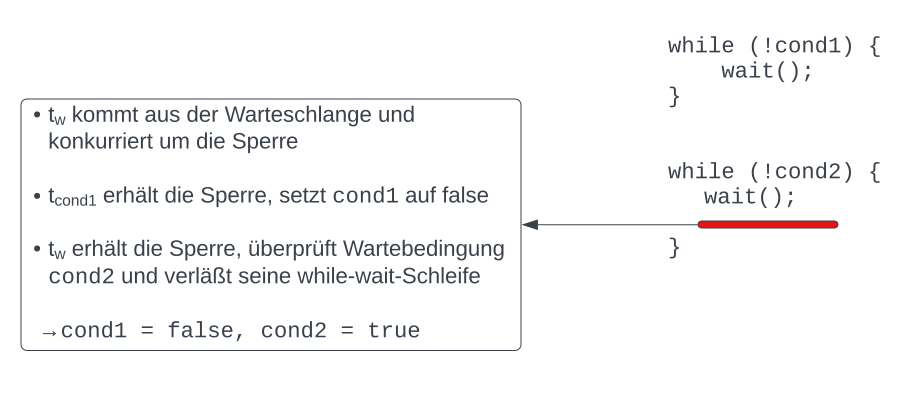
\includegraphics[scale=0.4]{chapters/Anhang/Klausuren/img/cond1cond2}
    \caption{in den rot markierten Bereich konkurriert $t_w$ um die Sperre des Objektes - wenn durch einen anderen Thread, der vor $t_w$ die Sperre erhält, \textit{cond1} auf \textit{false} gesetzt wird, stimmt die Ausgabe nicht mit der erwarteten überein. (Quelle: eigene)}
    \label{fig:cond1cond2}
\end{figure}

\noindent
Die korrekte Wartebedingung sollte lauten:

\begin{minted}[mathescape,
    linenos,
    numbersep=5pt,
    gobble=2,
    fontsize=\small,
    frame=lines,
    framesep=2mm]{java}
    public synchronized void cond1AndCond2() {
        while(!cond1 || !cond2) {
            try {
                wait();
            } catch(InterruptedException e) { }
        }
        System.out.println("cond1 and cond2:" + cond1 + " " + cond2);
    }
\end{minted}\\

Darüber hinaus müßte \code{notifyAll()} nur aufgerufen werden, wenn sowohl \code{cond1} als auch \code{cond2} auf \code{true} gesetzt sind, was leicht in den entsprechenden Methoden überprüft werden kann.
    \chapter{SS19}\label{ch:klausurss19}

\section{Aufgabe 1}

Bei der Aufgabe ist es wichtig, die Anforderungen genau zu beachten.\\
Ob eine Thread die while-wait-Schleife verlassen darf, wird von der Methode \code{tick()} gesteuert - wieviele Ticks ein Thread in der Schleife bleiben soll, wird von dem jeweiligen Thread definiert.\\
Die \code{tick()}-Methode wird von anderen Threads aufgerufen, es kann also durchaus vorkommen, dass mehrmals hintereinander
die \code{notifyAll()}-Methode aufgerufen wird - diese entfernt alle Threads aus der Warteschlange, damit die Threads ihre
Wartebedingungen erneut überprüfen können.\\
da \code{tick()} aber auch gleichzeitig einen Zähler realisieren soll, \textit{muss} es in der Methode auch eine Zählvariable geben, anhand derer die in der while-wait-Schleife enthaltenen Threads feststellen können, wie oft \code{tick()} aufgerufen wurde, um entsprechend aus der Schleife und nachfolgend der Methode herauszukommen.

\begin{figure}
    \centering
    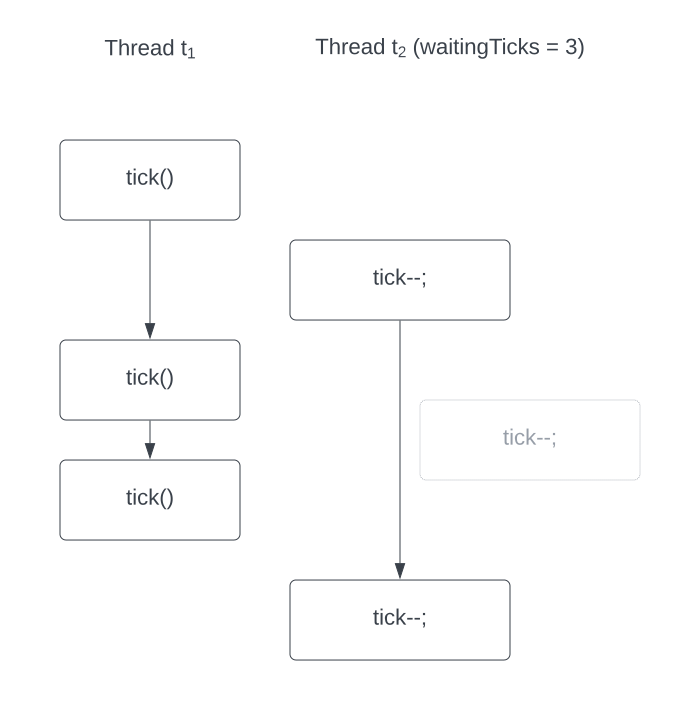
\includegraphics[scale=0.5]{chapters/Anhang/Klausuren/img/tick}
    \caption{Thread $t_1$ ruft 3 mal \texit{tick()} auf. Den Anforderungen nach müsste Thread $t_2$ danach aus der while-wait-Schleife herauskommen, erhält aber nicht die Sperre auf das Objekt von LogicalTime, um seinen eigenen Zähler rechtzeitig zu erniedrigen, bevor $t_1$ erneut \textit{tick()} aufruft. (Quelle: eigene)}
    \label{fig:tick}
\end{figure}

\section{Aufgabe 6}
Auch hier gilt, dass die Aufgabenstellung aufmerksam zu lesen ist.\\
Der Kreis soll erst ausgefüllt werden, wenn die Maustaste gelöst wird.

\begin{minted}[mathescape,
    linenos,
    numbersep=5pt,
    gobble=2,
    frame=lines,
    framesep=2mm]{java}
    private void mousePressed(double x, double y) {
        c = new Circle();
        c.setCenterX(x);
        c.setCenterY(y);
        c.setStroke(Color.RED);
        c.setFill(null); // oder Color.TRANSPARENT
        c.setRadius(RADIUS);
        graphicsPane.getChildren().add(c);
    }

    private void mouseReleased() {
        c.setFill(Color.RED);
        c = null;
    }
\end{minted}

\section{Aufgabe 8}

In der Abbildung \ref{fig:batchmodus} ist links der sequentielle Modus dargestellt, bei dem nach dem Senden einer Nachricht auf die Antwort des Servers gewartet wird, bevor eine neue Nachricht geschickt wird.
Dies wird i.d.R. verwendet, wenn das Senden einer neuen Nachricht abhängig ist von einem Ergebnis, die über die Server-Antwort übermittelt wird, oder wenn mit dem Server interagiert wird (Request abhängig vom Response).\\
Der Batch-Modus auf der rechten Seite der gleichen Abbildung ist schneller, da zwischen dem Senden von Nachrichten nicht auf Antworten gewartet werden müssen. \\
Erst nach dem Senden eine Batches von Nachrichten werden die dem Client zur Verfügung stehenden Antworten ausgelesen.\\

\noindent
In dieser Form des Batch-Modus besteht allerdings die Gefahr, dass es zu Verklemmungen kommt:
\begin{itemize}
    \item Bei dem Client kommen viele Nachrichten an, während er noch sendet.
    \item Die ankommenden Nachrichten für den Client werden gepuffert, bis sie ausgelesen werden (TCP- / OS-seitig).
    \item Läuft der Puffer voll, sorgt die Flusskontrolle (TCP) dafür, dass dem Sender mitgeteilt wird, dass keine Nachrichten mehr empfangen werden können, der Server sendet nicht mehr.
    \item Die zu sendenden Nachrichten des Servers werden in einen Puffer geschrieben.
    \item Der Sende-Puffer des Senders läuft voll.
    \item Bei dem nächsten Sende-Aufruf blockiert der Server, empfangene Nachrichten landen im Empfangspuffer
    \item Der Empfangspuffer des Servers läuft voll, der Client buffert die zu sendenden Nachrichten.
    \item Beide Anwendungen blockieren.
\end{itemize}

\\noindent
Um dieses Problem beim Batch-Modus zu umgehen, werden für das Senden und Empfangen zwei Threads auf Client-Seite erstellt: Ein Thread sendet, ein Thread empfängt. \\
Dadurch kann von dem Client immer wieder sein Empfangspuffer geleert werden, der Server wird beim Senden nicht blockiert.

\begin{figure}
    \centering
    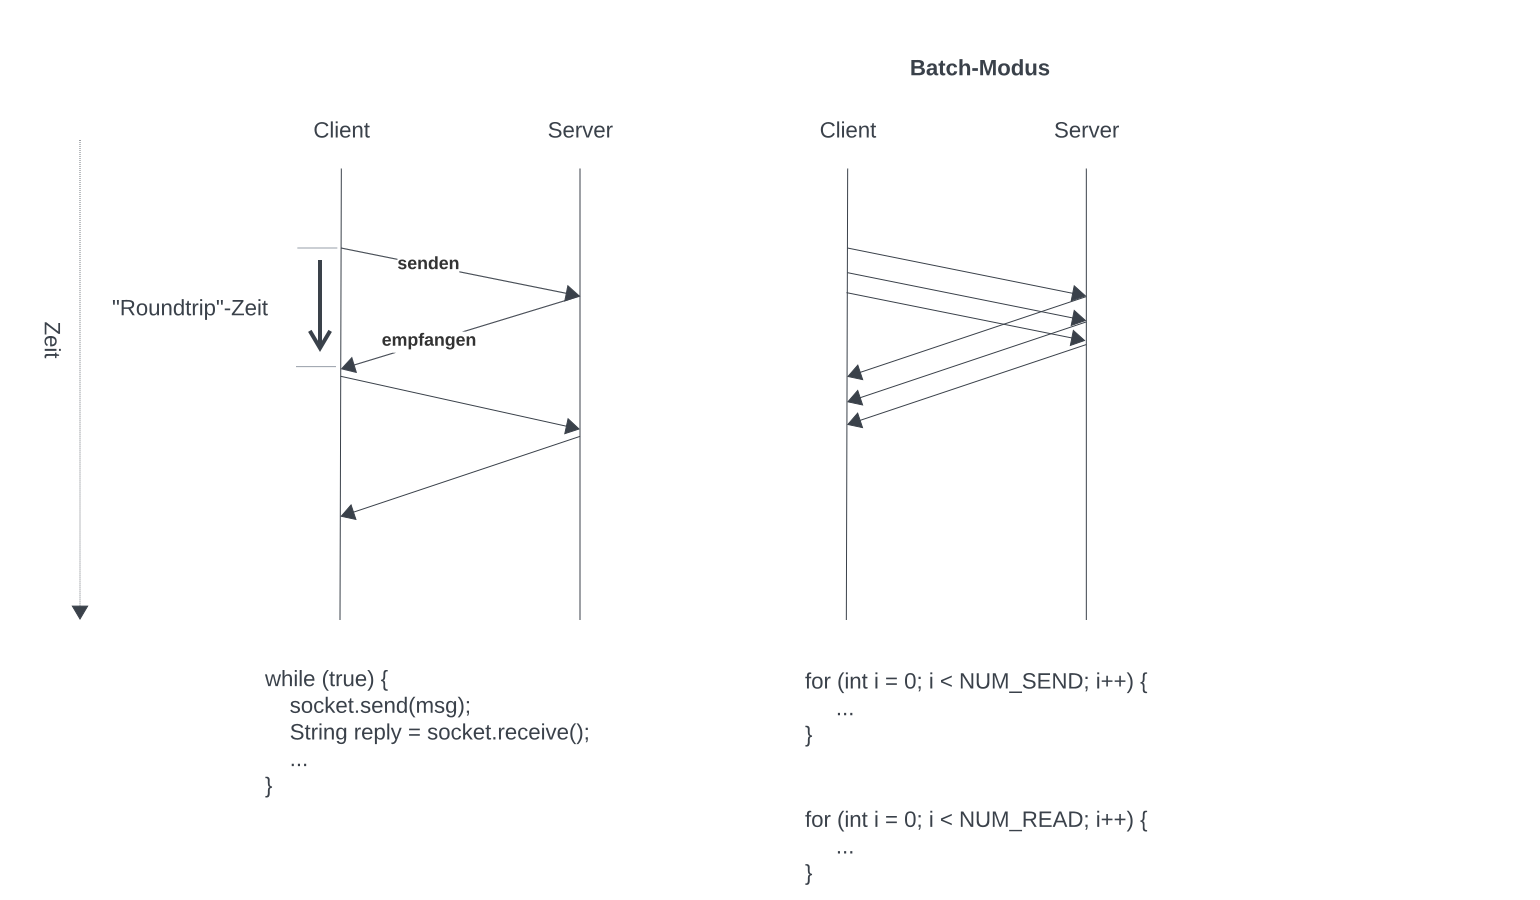
\includegraphics[scale=0.4]{chapters/Anhang/Klausuren/img/batchmodus}
    \caption{Vereinfachte Darstellung sequentieller Kommunikation und Batch-Modus (Quelle: eigene)}
    \label{fig:batchmodus}
\end{figure}
    
\begin{appendices}
    \input{chapters/Anhang/Zusatzaufgaben/index}
    \input{chapters/Anhang/Klausuren/ws13}
    \input{chapters/Anhang/Klausuren/ws15-16}
    \input{chapters/Anhang/Klausuren/ws16-17}
    \input{chapters/Anhang/Klausuren/ss19}
    \input{chapters/Anhang/Präsenzphase/index}

\end{appendices}


\end{appendices}


\end{appendices}



\begin{appendices}
    
\begin{appendices}
    
\begin{appendices}
    \input{chapters/Anhang/Zusatzaufgaben/index}
    \input{chapters/Anhang/Klausuren/ws13}
    \input{chapters/Anhang/Klausuren/ws15-16}
    \input{chapters/Anhang/Klausuren/ws16-17}
    \input{chapters/Anhang/Klausuren/ss19}
    \input{chapters/Anhang/Präsenzphase/index}

\end{appendices}

    \chapter{WS13}\label{ch:klausurws13}

\section{Aufgabe 1}
\subsection{Lösungsvorschlag}


\begin{minted}[mathescape,
    linenos,
    numbersep=5pt,
    gobble=2,
    fontsize=\small,
    frame=lines,
    framesep=2mm]{java}
    class Zahlenschloss {

        private int[] kombination;

        private int[] state;

        private boolean opened = false;

        public Zahlenschloss(int[] kombination) {
            this.kombination = kombination;
            this.state = new int[kombination.length];
        }

        public int anzahlRaedchen() {
            return kombination.length;
        }

        public synchronized int lesen(int radnummer) {
            return state[radnummer];
        }

        public synchronized void drehen(int radnummer, int zahl) {

            state[radnummer] = zahl;
            opened = true;
            for (int i = 0; i < anzahlRaedchen(); i++) {
                if (lesen(i) != kombination[i]) {
                    opened = false;
                    break;
                }
            }

            if (opened) {
                this.notify();
            }
        }

        public synchronized void warten() {

            while (!opened) {
                try {
                    this.wait();
                } catch (InterruptedException ignored) {}
            }
        }
    }
\end{minted}\\


\subsection{Anmerkung und Ergänzungen}

\begin{itemize}
    \item Es wird eine Wartebedingung benötigt, und zwar für die Methode \code{warten()}; ankommende Threads werden
    in die Warteschlange des Zahlenschloss-Objektes geschickt, wenn \code{opened} auf false gesetzt ist, ansonsten
    verlassen diese direkt die Methode wieder.\\
    Die Methode \code{drehen} benötigt keine separate Wartebedingung.
    Es reicht aus, sicherzustellen, dass das Zahlenschloss nicht gleichzeitig von anderen Threads benutzt werden kann:
    Die Methode \code{drehen} ist hierfür synchronisiert, damit das Zahlenschloss {insg.} immer nur eine Zustandsänderung
    erfährt - es sind andere Implementierungen möglich, in denen das Zahlenschloss dann von mehreren Threads gleichzeitig
    genutzt werden darf, wenn sich die Zugriffe anhand der ``Ziel``-\code{radnummer} unterscheiden, {bspw.} durch Mutex-Semaphore,
    die pro Radnummer verwendet werden\footnote{
        der gleichzeitige Zugriff auf unterschiedliche Arrays-Indizes ist erlaubt, s. `´17.4.1. Shared Variables``: \url{https://docs.oracle.com/javase/specs/jls/se21/html/jls-17.html#jls-1.4.1} - abgerufen 14.2.2024
    }.
    \item Es gibt nur eine Wartebedingung, von daher sollte \code{notify()} genügen.\\
    Wenn wir allerdings davon ausgehen, dass mehrere Threads über die Methode \code{warten()} in die Warteschlange des Objektes eingereiht worden sind,  sollte \code{notifyAll()} verwendet werden (siehe hierzu auch Abschnitt \ref{subsec:notifyAll}).
    Dennoch ist nicht garantiert, dass auch alle Threads aus der Warteschlange gelangen, denn es kann sein, dass ein anderer Thread die Methode \code{drehen()} betritt, dort die
    Zahlenkombination ändert und \code{opened} wieder auf \code{false} gesetzt wird. \\
    Ein anderer Thread, der nun in  \code{warten()} an die Reihe kommt, überprüft die Wartebedingung, und wird wieder in die Warteschlange eingereiht.
    Es ist also durchaus möglich, dass ein Thread nicht mehr aus der Methode \code{warten()} herauskommt.\\
    Dies könnte bspw. dadurch verhindert werden, dass die Threads in eine Queue gepackt werden, und in \code{drehen()} eine Wartebedingung eingefügt wird, die erst erfüllt ist,
    wenn die Queue geleert wurde oder aus ihr entnommen wurde, in der Reihenfolge, in der die Threads in die Queue eingereiht worden sind (\textit{FIFO}) (s. a. Abschnitt~\ref{subsec:readerwriterproblem}).
    \item Bei der Teilaufgabe mit der Schleife muss die komplette Schleife synchronisiert werden, was man durch ein \code{synchronized}-Statement erreicht\footnote{siehe Abschnitt~\ref{subsec:synchronizedstatement}.}
    \begin{minted}[mathescape,
        linenos,
        numbersep=5pt,
        gobble=2,
        fontsize=\small,
        frame=lines,
        framesep=2mm]{java}
        synchronized (zk) {
            for (int i = 0; i < anzahlRaedchen; i++) {
                System.out.println(zk.lesen(i));
            }
        }
    \end{minted}
    Ansonsten läuft man Gefahr, dass sich nach Auslesen der 1. Position der Wert von Position 2 geändert hat und dadurch eine
    Zahlenkombination ausgegeben wird, die es nicht gegeben hat:
    \begin{enumerate}
        \item $K\coloneqq[0, 0, 0]$
        \item Position $K_0$ wird ausgelesen und liefert $0$.
        \item Thread ändert $K_0$ zu $1$ $\implies K\coloneqq[1, 0, 0] $.
        \item Thread ändert $K_1$ zu $2$ $\implies K\coloneqq[1, 2, 0] $.
        \item Thread ändert $K_2$ zu $3$ $\implies K\coloneqq[1, 2, 3] $.
        \item Positionen $K_1$ und $K_2$ werden ausgelesen und liefern: $2, 3$
        \item Ausgabe: $0, 2, 3$ - diese Kombination hat es in dem Fall aber tatsächlich nicht gegeben.
    \end{enumerate}
\end{itemize}

\begin{tcolorbox}[colback=red!20,color=white,title=Anmerkung]
    Die Methode \code{lesen()} als \code{synchronized} zu markieren könnte man sich vlt. sparen, wenn man davon ausgeht,
    dass die Methode ohnehin in einem \code{synchronized}-Statement verwendet wird, um alle Rädchen abzulesen.\\
    Mehrere Threads können also nicht parallel auf unterschiedliche Positionen des Feldes zugreifen, wenn die Methode
    synchronisiert ist.\\
    Allerdings ist sowohl das Skript als auch das Buch recht klar, was in dieser Situation geschehen muss (s. Skript Fopt1/2, S. 9, außerdem \cite[31, Abschnitt 2.3.6]{Oec22}): Es muss (in diesem Kurs) immer \code{synchronized} verwendet werden, wenn gleichzeitig
    Daten geschrieben und gleichzeitig diese Daten gelesen werden sollen - und eine andere Implementierung, bei der die
    einzelnen Positionen ``gelocked`` sind, so dass ein gleichzeitiger Zugriff auf unterschiedliche Rädchen möglich ist, war nicht gefordert.\\
    Ggfl. würde in anderen Implementierungen der Einsatz von \code{AtomicReferenceArray}\footnote{s. \cite[157 ff.]{Oec22}
    s. ``Class AtomicReferenceArray<E>``: \url{https://docs.oracle.com/en/java/javase/21/docs/api/java.base/java/util/concurrent/atomic/AtomicReferenceArray.html} - abgerufen 15.2.2024
    } Sinn machen, aber das Lehrmaterial ist bereits sehr eindeutig bzgl. der Verwendung von \code{synchronized}.
\end{tcolorbox}



\section{Aufgabe 3}
\subsection{Lösungsvorschlag}

\subsection*{Statische Parallelität}
Statische Parallelität erlaubt es einem Server, eine \textit{fixe} Anzahl von Verbindungen gleichzeitig zu bedienen.\\
Hierbei wird ein Feld von Threads erstellt, wobei jeder Thread das \code{ServerSocket}-Objekt als Referenz übergeben bekommt.
In der \code{run()}-Methode wird dann über \code{accept()} in einer Endlosschleife auf eingehende Verbindungen gewartet, die dann so lange bedient werden, bis sich ein Client wieder abmeldet (oder eine andere Abbruchbedingung erfüllt ist, wie z.B. ein \code{SocketTimeout}).\\
Das sich ein Client abmeldet, bekommt man bspw. dadurch mit, dass \code{null} beim Lesen von einer Nachricht des Clients zurückgegeben wird (vgl. \cite[286]{Oec22}. \\
Siehe Abschnitt~\ref{sec:seqparserver} für ein Implementierungsbeispiel.



\subsection*{Dynamische Parallelität}

Bei der \textbf{Dynamischer Parallelität} erzeugt der Server für jede Verbindung einen neuen Thread, der so lange läuft, bis der Client die Verbindung wieder trennt.\\
Die Anzahl der Threads ändert sich dadurch laufend.\\
Wird die max. Anzahl erlaubter Threads nicht kontrolliert, kann es zu einer Überlastung des Server-Rechners kommen (bspw. durch einen Denial-of-Service-Angriff.)\\

\noindent
I.d.R. ist eine Mischform aus beidem geeignet, um mehrere Clients gleichzeitig bedienen zu können, und dabei nicht Gefahr zu laufen, durch dynamisches, unbegrenztes Wachstum der Anzahl der Threads überlastet zu werden.

    \chapter{WS13}\label{ch:klausurws5-16}

\section{Rechteck-Scroll (SS15 Aufgabe 2)}

Aufgabenstellung unklar.\\
Mögliche Implementierung unter \url{https://github.com/ThorstenSuckow/fopt/tree/main/src/main/java/klausurvorbereitung/foptws1516/MouseDragsSquareDemo}.

\section{Rechteck-Scroll (WS15/16 Aufgabe 1)}

Aufgabenstellung unklar.\\
Mögliche Implementierung unter \url{https://github.com/ThorstenSuckow/fopt/tree/main/src/main/java/klausurvorbereitung/foptws1516/MaxWeightDemo}.\\

\noindent
Es gibt nur eine Warteschlange für Threads in \code{use()}, es gibt keine Wartebedingung in \code{dontUse()} und damit auch keine weitere Warteschlange.\\
Es sind durch die Zugriffe auf unterschiedliche Indizes allerdings mehrere Wartebedingungen vorhanden, weshalb hab \code{notifyAll()} nutzen sollte,
sobald ein Zugriff auf ein Feld nach Aufruf von \code{dontUse} wieder möglich wird.\\
Ansonsten bestünde die Gefahr, dass bei dem Einsatz von \code{notify()} ein wartender Thread nicht geweckt wird, obwohl er weiterlaufen könnte:\\
Angenommen, das Feld $F$ hat eine Länge von $3$, das \code{maxWeight} ist mit $2$ konfiguriert.
Thread $t_1$ mit einer Laufzeit von $200\ sek$ bekommt Zugriff auf $F_0$, setzt $currentWeight$ auf $1$.\\
Thread $t_2$ mit einer Laufzeit von $1\ sek$ möchte auf $F_1$ zugreifen, setzt $currentWeight=2$ in die Warteschlange.\\
Thread $t_3$ meldet Zugriff auf $F_0$ an und gelangt in die Warteschlange.\\
Thread $t_4$ meldet Zugriff auf $F_1$ an und gelangt in die Warteschlange.\\
Thread $t_2$ ist mit der Bearbeitung von $F_1$ fertig, $currentWeight$ wird auf $1$ gesetzt, \code{notify()} wird aufgerufen.\\
Thread $t_3$ wird aus der Warteschlange geholt, kann aber nicht weiterarbeiten, da $F_0$ noch durch den länger dauernden $t_1$ blockiert ist, und kommt wieder in die Warteschlange.\\

\noindent
Offensichtlich hätte in dem Beispiel \code{notifyAll()} dazu geführt, dass auch $T_4$ seine Wartebedingung hätte überprüfen können, und hätte so Zugriff auf $F_1$ bekommen.
Stattdessen muss nun gewartet werden, bis das nächste \code{notify()} aufgerufen wird, oder ein neu ankommender Thread $F_1$ belegt.

    \chapter{WS16-17}\label{ch:klausurws16-17}

\section{Aufgabe 1}
\subsection{Lösungshinweis}

Die erste Aufgabe verdeutlicht, was bei einem \code{notifyAll()} und unsauber gesetzten Wartebedingungen passieren kann.\\
Sei folgender Quellcode gegeben:


\begin{minted}[mathescape,
    linenos,
    numbersep=5pt,
    gobble=2,
    fontsize=\small,
    frame=lines,
    framesep=2mm]{java}
    class Cond1AndCond2 {

        private boolean cond1;
        private boolean cond2;

        public synchronized void setCond1(boolean c) {
            cond1 = c;
            notifyAll();
        }

        public synchronized void setCond2(boolean c) {
            cond2 = c;
            notifyAll();
        }

        public synchronized void cond1AndCond2() {
            while(!cond1) {
                try {
                    wait();
                } catch(InterruptedException e) { }
            }

            while(!cond2) {
                try {
                    wait();
                } catch(InterruptedException e) {}
            }
            System.out.println("cond1 and cond2:" + cond1 + " " + cond2);
        }
    }
\end{minted}\\

Man sollte auf den ersten Blick meinen, dass \code{cond1} und \code{cond2} beide \code{true} sein müssen, damit die Ausgabe erfolgt.\\
Tatsächlich ist es aber so, dass es in der Methode zwei unterschiedliche Wartebedingungen gibt.\\
Die erste Wartebedingung schickt einen Thread in die Warteschlange, wenn \code{cond1 == false} gilt.\\
Setzt ein anderer Thread über \code{setCond1(true)} das Attribut entsprechend auf \code{true}, bewirkt der nachfolgende Aufruf von \code{notifyAll()}, dass alle \textit{wartenden} Threads aus der Warteschlange entfernt werden und erneut um eine Sperre des Objektes konkurrieren.\\
Erhält ein entsprechender Thread $t_w$ die Sperre auf das Objekt und kann seine \textit{while-wait-Schleife} verlassen, kann es vorkommen, dass er erneut in die Warteschlange eingereiht wird, wegen der nachfolgenden Wartebedingung \code{cond2 == false}.\\
Angenommen, ein weiterer Thread ruft nun \code{setCond2(true)} auf, und $t_w$ kommt aus der Warteschlange und konkurriert erneut und um die Sperre des Objektes, dann kann es vorkommen, das ein anderer Thread zunächst die Sperre erhält, \code{cond1} wieder auf \code{false} setzt, dann erhält $t_w$ die Sperre, überprüft die Wartebedingung \code{cond2 == false}.\\
Wegen \code{cond2} gelangt er aus der \textit{while-wait-Schleife} und die Ausgabe erfolgt - da zwischenzeitlich \code{cond1} wieder auf \code{false} gesetzt wurde, ist die erwartete Ausgabe nicht \code{true true}, sondern \code{false true} (s. Abbildung \ref{fig:cond1cond2}).\\

\begin{figure}
    \centering
    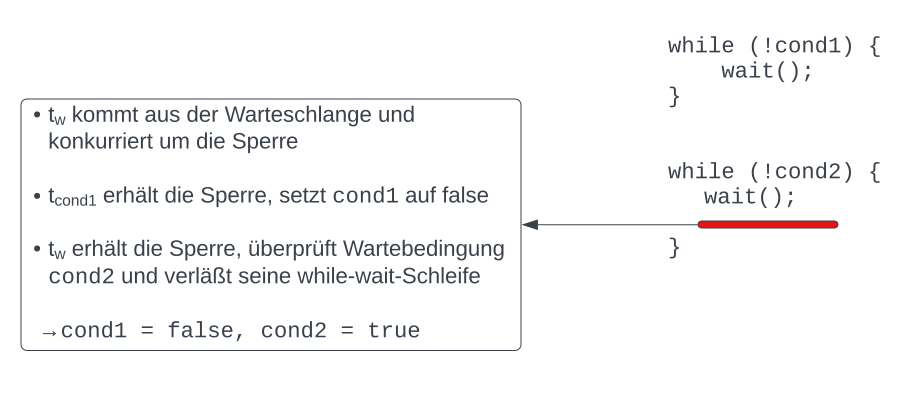
\includegraphics[scale=0.4]{chapters/Anhang/Klausuren/img/cond1cond2}
    \caption{in den rot markierten Bereich konkurriert $t_w$ um die Sperre des Objektes - wenn durch einen anderen Thread, der vor $t_w$ die Sperre erhält, \textit{cond1} auf \textit{false} gesetzt wird, stimmt die Ausgabe nicht mit der erwarteten überein. (Quelle: eigene)}
    \label{fig:cond1cond2}
\end{figure}

\noindent
Die korrekte Wartebedingung sollte lauten:

\begin{minted}[mathescape,
    linenos,
    numbersep=5pt,
    gobble=2,
    fontsize=\small,
    frame=lines,
    framesep=2mm]{java}
    public synchronized void cond1AndCond2() {
        while(!cond1 || !cond2) {
            try {
                wait();
            } catch(InterruptedException e) { }
        }
        System.out.println("cond1 and cond2:" + cond1 + " " + cond2);
    }
\end{minted}\\

Darüber hinaus müßte \code{notifyAll()} nur aufgerufen werden, wenn sowohl \code{cond1} als auch \code{cond2} auf \code{true} gesetzt sind, was leicht in den entsprechenden Methoden überprüft werden kann.
    \chapter{SS19}\label{ch:klausurss19}

\section{Aufgabe 1}

Bei der Aufgabe ist es wichtig, die Anforderungen genau zu beachten.\\
Ob eine Thread die while-wait-Schleife verlassen darf, wird von der Methode \code{tick()} gesteuert - wieviele Ticks ein Thread in der Schleife bleiben soll, wird von dem jeweiligen Thread definiert.\\
Die \code{tick()}-Methode wird von anderen Threads aufgerufen, es kann also durchaus vorkommen, dass mehrmals hintereinander
die \code{notifyAll()}-Methode aufgerufen wird - diese entfernt alle Threads aus der Warteschlange, damit die Threads ihre
Wartebedingungen erneut überprüfen können.\\
da \code{tick()} aber auch gleichzeitig einen Zähler realisieren soll, \textit{muss} es in der Methode auch eine Zählvariable geben, anhand derer die in der while-wait-Schleife enthaltenen Threads feststellen können, wie oft \code{tick()} aufgerufen wurde, um entsprechend aus der Schleife und nachfolgend der Methode herauszukommen.

\begin{figure}
    \centering
    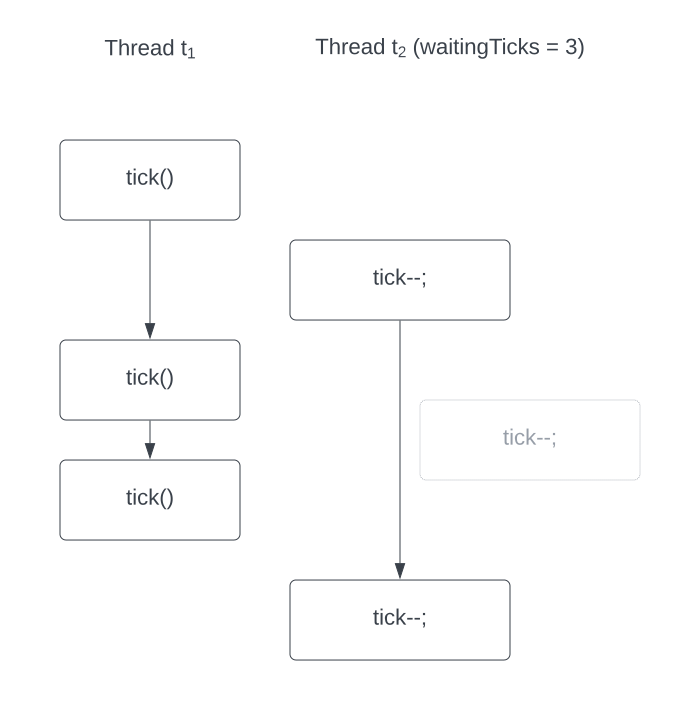
\includegraphics[scale=0.5]{chapters/Anhang/Klausuren/img/tick}
    \caption{Thread $t_1$ ruft 3 mal \texit{tick()} auf. Den Anforderungen nach müsste Thread $t_2$ danach aus der while-wait-Schleife herauskommen, erhält aber nicht die Sperre auf das Objekt von LogicalTime, um seinen eigenen Zähler rechtzeitig zu erniedrigen, bevor $t_1$ erneut \textit{tick()} aufruft. (Quelle: eigene)}
    \label{fig:tick}
\end{figure}

\section{Aufgabe 6}
Auch hier gilt, dass die Aufgabenstellung aufmerksam zu lesen ist.\\
Der Kreis soll erst ausgefüllt werden, wenn die Maustaste gelöst wird.

\begin{minted}[mathescape,
    linenos,
    numbersep=5pt,
    gobble=2,
    frame=lines,
    framesep=2mm]{java}
    private void mousePressed(double x, double y) {
        c = new Circle();
        c.setCenterX(x);
        c.setCenterY(y);
        c.setStroke(Color.RED);
        c.setFill(null); // oder Color.TRANSPARENT
        c.setRadius(RADIUS);
        graphicsPane.getChildren().add(c);
    }

    private void mouseReleased() {
        c.setFill(Color.RED);
        c = null;
    }
\end{minted}

\section{Aufgabe 8}

In der Abbildung \ref{fig:batchmodus} ist links der sequentielle Modus dargestellt, bei dem nach dem Senden einer Nachricht auf die Antwort des Servers gewartet wird, bevor eine neue Nachricht geschickt wird.
Dies wird i.d.R. verwendet, wenn das Senden einer neuen Nachricht abhängig ist von einem Ergebnis, die über die Server-Antwort übermittelt wird, oder wenn mit dem Server interagiert wird (Request abhängig vom Response).\\
Der Batch-Modus auf der rechten Seite der gleichen Abbildung ist schneller, da zwischen dem Senden von Nachrichten nicht auf Antworten gewartet werden müssen. \\
Erst nach dem Senden eine Batches von Nachrichten werden die dem Client zur Verfügung stehenden Antworten ausgelesen.\\

\noindent
In dieser Form des Batch-Modus besteht allerdings die Gefahr, dass es zu Verklemmungen kommt:
\begin{itemize}
    \item Bei dem Client kommen viele Nachrichten an, während er noch sendet.
    \item Die ankommenden Nachrichten für den Client werden gepuffert, bis sie ausgelesen werden (TCP- / OS-seitig).
    \item Läuft der Puffer voll, sorgt die Flusskontrolle (TCP) dafür, dass dem Sender mitgeteilt wird, dass keine Nachrichten mehr empfangen werden können, der Server sendet nicht mehr.
    \item Die zu sendenden Nachrichten des Servers werden in einen Puffer geschrieben.
    \item Der Sende-Puffer des Senders läuft voll.
    \item Bei dem nächsten Sende-Aufruf blockiert der Server, empfangene Nachrichten landen im Empfangspuffer
    \item Der Empfangspuffer des Servers läuft voll, der Client buffert die zu sendenden Nachrichten.
    \item Beide Anwendungen blockieren.
\end{itemize}

\\noindent
Um dieses Problem beim Batch-Modus zu umgehen, werden für das Senden und Empfangen zwei Threads auf Client-Seite erstellt: Ein Thread sendet, ein Thread empfängt. \\
Dadurch kann von dem Client immer wieder sein Empfangspuffer geleert werden, der Server wird beim Senden nicht blockiert.

\begin{figure}
    \centering
    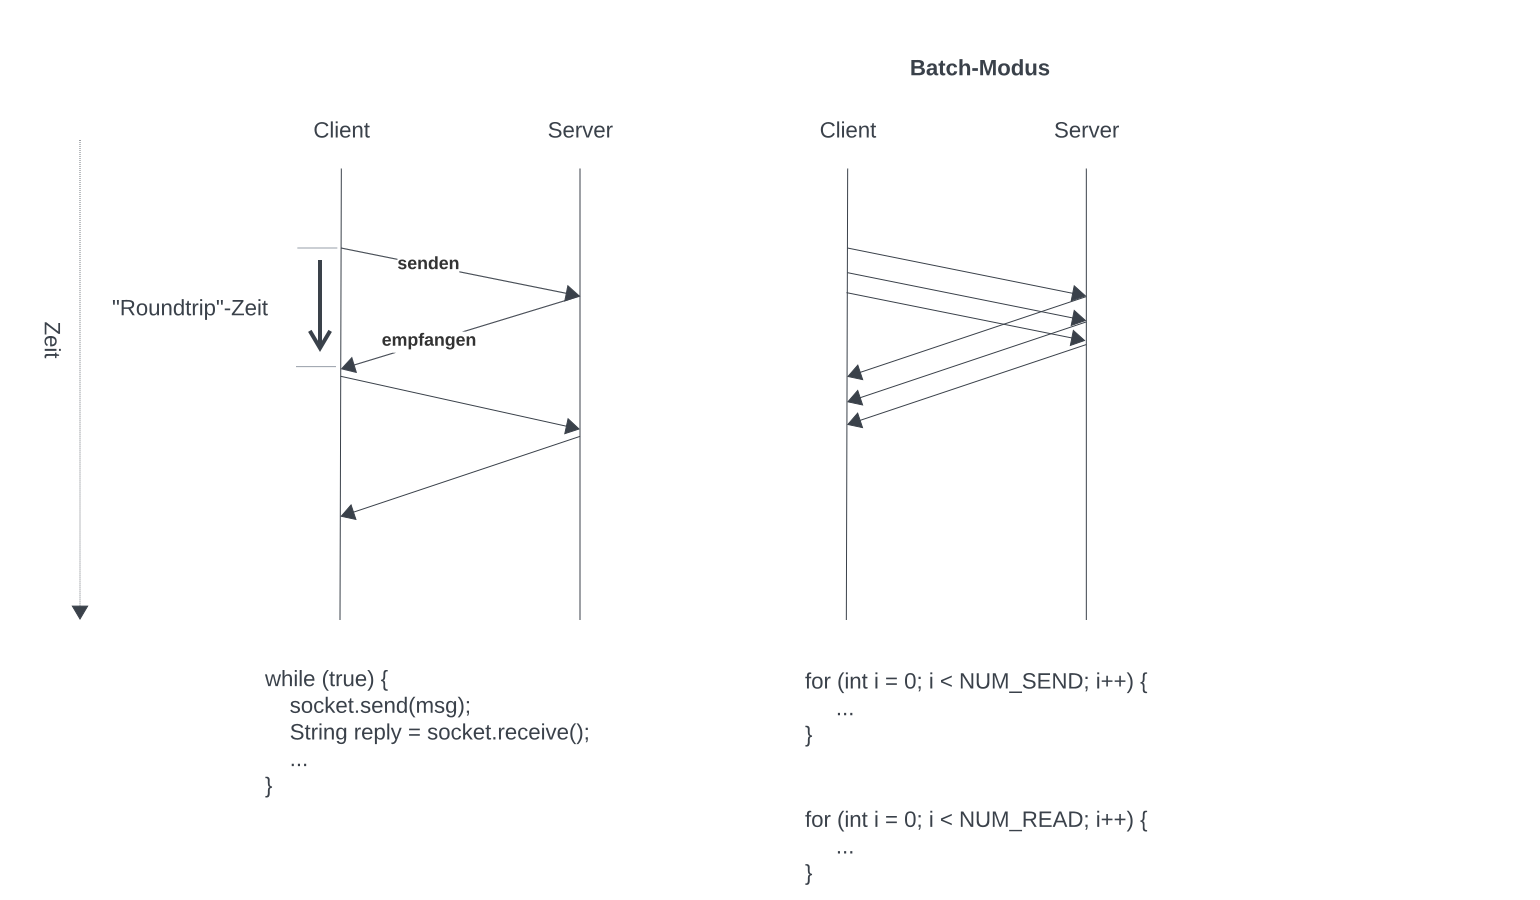
\includegraphics[scale=0.4]{chapters/Anhang/Klausuren/img/batchmodus}
    \caption{Vereinfachte Darstellung sequentieller Kommunikation und Batch-Modus (Quelle: eigene)}
    \label{fig:batchmodus}
\end{figure}
    
\begin{appendices}
    \input{chapters/Anhang/Zusatzaufgaben/index}
    \input{chapters/Anhang/Klausuren/ws13}
    \input{chapters/Anhang/Klausuren/ws15-16}
    \input{chapters/Anhang/Klausuren/ws16-17}
    \input{chapters/Anhang/Klausuren/ss19}
    \input{chapters/Anhang/Präsenzphase/index}

\end{appendices}


\end{appendices}

    \chapter{WS13}\label{ch:klausurws13}

\section{Aufgabe 1}
\subsection{Lösungsvorschlag}


\begin{minted}[mathescape,
    linenos,
    numbersep=5pt,
    gobble=2,
    fontsize=\small,
    frame=lines,
    framesep=2mm]{java}
    class Zahlenschloss {

        private int[] kombination;

        private int[] state;

        private boolean opened = false;

        public Zahlenschloss(int[] kombination) {
            this.kombination = kombination;
            this.state = new int[kombination.length];
        }

        public int anzahlRaedchen() {
            return kombination.length;
        }

        public synchronized int lesen(int radnummer) {
            return state[radnummer];
        }

        public synchronized void drehen(int radnummer, int zahl) {

            state[radnummer] = zahl;
            opened = true;
            for (int i = 0; i < anzahlRaedchen(); i++) {
                if (lesen(i) != kombination[i]) {
                    opened = false;
                    break;
                }
            }

            if (opened) {
                this.notify();
            }
        }

        public synchronized void warten() {

            while (!opened) {
                try {
                    this.wait();
                } catch (InterruptedException ignored) {}
            }
        }
    }
\end{minted}\\


\subsection{Anmerkung und Ergänzungen}

\begin{itemize}
    \item Es wird eine Wartebedingung benötigt, und zwar für die Methode \code{warten()}; ankommende Threads werden
    in die Warteschlange des Zahlenschloss-Objektes geschickt, wenn \code{opened} auf false gesetzt ist, ansonsten
    verlassen diese direkt die Methode wieder.\\
    Die Methode \code{drehen} benötigt keine separate Wartebedingung.
    Es reicht aus, sicherzustellen, dass das Zahlenschloss nicht gleichzeitig von anderen Threads benutzt werden kann:
    Die Methode \code{drehen} ist hierfür synchronisiert, damit das Zahlenschloss {insg.} immer nur eine Zustandsänderung
    erfährt - es sind andere Implementierungen möglich, in denen das Zahlenschloss dann von mehreren Threads gleichzeitig
    genutzt werden darf, wenn sich die Zugriffe anhand der ``Ziel``-\code{radnummer} unterscheiden, {bspw.} durch Mutex-Semaphore,
    die pro Radnummer verwendet werden\footnote{
        der gleichzeitige Zugriff auf unterschiedliche Arrays-Indizes ist erlaubt, s. `´17.4.1. Shared Variables``: \url{https://docs.oracle.com/javase/specs/jls/se21/html/jls-17.html#jls-1.4.1} - abgerufen 14.2.2024
    }.
    \item Es gibt nur eine Wartebedingung, von daher sollte \code{notify()} genügen.\\
    Wenn wir allerdings davon ausgehen, dass mehrere Threads über die Methode \code{warten()} in die Warteschlange des Objektes eingereiht worden sind,  sollte \code{notifyAll()} verwendet werden (siehe hierzu auch Abschnitt \ref{subsec:notifyAll}).
    Dennoch ist nicht garantiert, dass auch alle Threads aus der Warteschlange gelangen, denn es kann sein, dass ein anderer Thread die Methode \code{drehen()} betritt, dort die
    Zahlenkombination ändert und \code{opened} wieder auf \code{false} gesetzt wird. \\
    Ein anderer Thread, der nun in  \code{warten()} an die Reihe kommt, überprüft die Wartebedingung, und wird wieder in die Warteschlange eingereiht.
    Es ist also durchaus möglich, dass ein Thread nicht mehr aus der Methode \code{warten()} herauskommt.\\
    Dies könnte bspw. dadurch verhindert werden, dass die Threads in eine Queue gepackt werden, und in \code{drehen()} eine Wartebedingung eingefügt wird, die erst erfüllt ist,
    wenn die Queue geleert wurde oder aus ihr entnommen wurde, in der Reihenfolge, in der die Threads in die Queue eingereiht worden sind (\textit{FIFO}) (s. a. Abschnitt~\ref{subsec:readerwriterproblem}).
    \item Bei der Teilaufgabe mit der Schleife muss die komplette Schleife synchronisiert werden, was man durch ein \code{synchronized}-Statement erreicht\footnote{siehe Abschnitt~\ref{subsec:synchronizedstatement}.}
    \begin{minted}[mathescape,
        linenos,
        numbersep=5pt,
        gobble=2,
        fontsize=\small,
        frame=lines,
        framesep=2mm]{java}
        synchronized (zk) {
            for (int i = 0; i < anzahlRaedchen; i++) {
                System.out.println(zk.lesen(i));
            }
        }
    \end{minted}
    Ansonsten läuft man Gefahr, dass sich nach Auslesen der 1. Position der Wert von Position 2 geändert hat und dadurch eine
    Zahlenkombination ausgegeben wird, die es nicht gegeben hat:
    \begin{enumerate}
        \item $K\coloneqq[0, 0, 0]$
        \item Position $K_0$ wird ausgelesen und liefert $0$.
        \item Thread ändert $K_0$ zu $1$ $\implies K\coloneqq[1, 0, 0] $.
        \item Thread ändert $K_1$ zu $2$ $\implies K\coloneqq[1, 2, 0] $.
        \item Thread ändert $K_2$ zu $3$ $\implies K\coloneqq[1, 2, 3] $.
        \item Positionen $K_1$ und $K_2$ werden ausgelesen und liefern: $2, 3$
        \item Ausgabe: $0, 2, 3$ - diese Kombination hat es in dem Fall aber tatsächlich nicht gegeben.
    \end{enumerate}
\end{itemize}

\begin{tcolorbox}[colback=red!20,color=white,title=Anmerkung]
    Die Methode \code{lesen()} als \code{synchronized} zu markieren könnte man sich vlt. sparen, wenn man davon ausgeht,
    dass die Methode ohnehin in einem \code{synchronized}-Statement verwendet wird, um alle Rädchen abzulesen.\\
    Mehrere Threads können also nicht parallel auf unterschiedliche Positionen des Feldes zugreifen, wenn die Methode
    synchronisiert ist.\\
    Allerdings ist sowohl das Skript als auch das Buch recht klar, was in dieser Situation geschehen muss (s. Skript Fopt1/2, S. 9, außerdem \cite[31, Abschnitt 2.3.6]{Oec22}): Es muss (in diesem Kurs) immer \code{synchronized} verwendet werden, wenn gleichzeitig
    Daten geschrieben und gleichzeitig diese Daten gelesen werden sollen - und eine andere Implementierung, bei der die
    einzelnen Positionen ``gelocked`` sind, so dass ein gleichzeitiger Zugriff auf unterschiedliche Rädchen möglich ist, war nicht gefordert.\\
    Ggfl. würde in anderen Implementierungen der Einsatz von \code{AtomicReferenceArray}\footnote{s. \cite[157 ff.]{Oec22}
    s. ``Class AtomicReferenceArray<E>``: \url{https://docs.oracle.com/en/java/javase/21/docs/api/java.base/java/util/concurrent/atomic/AtomicReferenceArray.html} - abgerufen 15.2.2024
    } Sinn machen, aber das Lehrmaterial ist bereits sehr eindeutig bzgl. der Verwendung von \code{synchronized}.
\end{tcolorbox}



\section{Aufgabe 3}
\subsection{Lösungsvorschlag}

\subsection*{Statische Parallelität}
Statische Parallelität erlaubt es einem Server, eine \textit{fixe} Anzahl von Verbindungen gleichzeitig zu bedienen.\\
Hierbei wird ein Feld von Threads erstellt, wobei jeder Thread das \code{ServerSocket}-Objekt als Referenz übergeben bekommt.
In der \code{run()}-Methode wird dann über \code{accept()} in einer Endlosschleife auf eingehende Verbindungen gewartet, die dann so lange bedient werden, bis sich ein Client wieder abmeldet (oder eine andere Abbruchbedingung erfüllt ist, wie z.B. ein \code{SocketTimeout}).\\
Das sich ein Client abmeldet, bekommt man bspw. dadurch mit, dass \code{null} beim Lesen von einer Nachricht des Clients zurückgegeben wird (vgl. \cite[286]{Oec22}. \\
Siehe Abschnitt~\ref{sec:seqparserver} für ein Implementierungsbeispiel.



\subsection*{Dynamische Parallelität}

Bei der \textbf{Dynamischer Parallelität} erzeugt der Server für jede Verbindung einen neuen Thread, der so lange läuft, bis der Client die Verbindung wieder trennt.\\
Die Anzahl der Threads ändert sich dadurch laufend.\\
Wird die max. Anzahl erlaubter Threads nicht kontrolliert, kann es zu einer Überlastung des Server-Rechners kommen (bspw. durch einen Denial-of-Service-Angriff.)\\

\noindent
I.d.R. ist eine Mischform aus beidem geeignet, um mehrere Clients gleichzeitig bedienen zu können, und dabei nicht Gefahr zu laufen, durch dynamisches, unbegrenztes Wachstum der Anzahl der Threads überlastet zu werden.

    \chapter{WS13}\label{ch:klausurws5-16}

\section{Rechteck-Scroll (SS15 Aufgabe 2)}

Aufgabenstellung unklar.\\
Mögliche Implementierung unter \url{https://github.com/ThorstenSuckow/fopt/tree/main/src/main/java/klausurvorbereitung/foptws1516/MouseDragsSquareDemo}.

\section{Rechteck-Scroll (WS15/16 Aufgabe 1)}

Aufgabenstellung unklar.\\
Mögliche Implementierung unter \url{https://github.com/ThorstenSuckow/fopt/tree/main/src/main/java/klausurvorbereitung/foptws1516/MaxWeightDemo}.\\

\noindent
Es gibt nur eine Warteschlange für Threads in \code{use()}, es gibt keine Wartebedingung in \code{dontUse()} und damit auch keine weitere Warteschlange.\\
Es sind durch die Zugriffe auf unterschiedliche Indizes allerdings mehrere Wartebedingungen vorhanden, weshalb hab \code{notifyAll()} nutzen sollte,
sobald ein Zugriff auf ein Feld nach Aufruf von \code{dontUse} wieder möglich wird.\\
Ansonsten bestünde die Gefahr, dass bei dem Einsatz von \code{notify()} ein wartender Thread nicht geweckt wird, obwohl er weiterlaufen könnte:\\
Angenommen, das Feld $F$ hat eine Länge von $3$, das \code{maxWeight} ist mit $2$ konfiguriert.
Thread $t_1$ mit einer Laufzeit von $200\ sek$ bekommt Zugriff auf $F_0$, setzt $currentWeight$ auf $1$.\\
Thread $t_2$ mit einer Laufzeit von $1\ sek$ möchte auf $F_1$ zugreifen, setzt $currentWeight=2$ in die Warteschlange.\\
Thread $t_3$ meldet Zugriff auf $F_0$ an und gelangt in die Warteschlange.\\
Thread $t_4$ meldet Zugriff auf $F_1$ an und gelangt in die Warteschlange.\\
Thread $t_2$ ist mit der Bearbeitung von $F_1$ fertig, $currentWeight$ wird auf $1$ gesetzt, \code{notify()} wird aufgerufen.\\
Thread $t_3$ wird aus der Warteschlange geholt, kann aber nicht weiterarbeiten, da $F_0$ noch durch den länger dauernden $t_1$ blockiert ist, und kommt wieder in die Warteschlange.\\

\noindent
Offensichtlich hätte in dem Beispiel \code{notifyAll()} dazu geführt, dass auch $T_4$ seine Wartebedingung hätte überprüfen können, und hätte so Zugriff auf $F_1$ bekommen.
Stattdessen muss nun gewartet werden, bis das nächste \code{notify()} aufgerufen wird, oder ein neu ankommender Thread $F_1$ belegt.

    \chapter{WS16-17}\label{ch:klausurws16-17}

\section{Aufgabe 1}
\subsection{Lösungshinweis}

Die erste Aufgabe verdeutlicht, was bei einem \code{notifyAll()} und unsauber gesetzten Wartebedingungen passieren kann.\\
Sei folgender Quellcode gegeben:


\begin{minted}[mathescape,
    linenos,
    numbersep=5pt,
    gobble=2,
    fontsize=\small,
    frame=lines,
    framesep=2mm]{java}
    class Cond1AndCond2 {

        private boolean cond1;
        private boolean cond2;

        public synchronized void setCond1(boolean c) {
            cond1 = c;
            notifyAll();
        }

        public synchronized void setCond2(boolean c) {
            cond2 = c;
            notifyAll();
        }

        public synchronized void cond1AndCond2() {
            while(!cond1) {
                try {
                    wait();
                } catch(InterruptedException e) { }
            }

            while(!cond2) {
                try {
                    wait();
                } catch(InterruptedException e) {}
            }
            System.out.println("cond1 and cond2:" + cond1 + " " + cond2);
        }
    }
\end{minted}\\

Man sollte auf den ersten Blick meinen, dass \code{cond1} und \code{cond2} beide \code{true} sein müssen, damit die Ausgabe erfolgt.\\
Tatsächlich ist es aber so, dass es in der Methode zwei unterschiedliche Wartebedingungen gibt.\\
Die erste Wartebedingung schickt einen Thread in die Warteschlange, wenn \code{cond1 == false} gilt.\\
Setzt ein anderer Thread über \code{setCond1(true)} das Attribut entsprechend auf \code{true}, bewirkt der nachfolgende Aufruf von \code{notifyAll()}, dass alle \textit{wartenden} Threads aus der Warteschlange entfernt werden und erneut um eine Sperre des Objektes konkurrieren.\\
Erhält ein entsprechender Thread $t_w$ die Sperre auf das Objekt und kann seine \textit{while-wait-Schleife} verlassen, kann es vorkommen, dass er erneut in die Warteschlange eingereiht wird, wegen der nachfolgenden Wartebedingung \code{cond2 == false}.\\
Angenommen, ein weiterer Thread ruft nun \code{setCond2(true)} auf, und $t_w$ kommt aus der Warteschlange und konkurriert erneut und um die Sperre des Objektes, dann kann es vorkommen, das ein anderer Thread zunächst die Sperre erhält, \code{cond1} wieder auf \code{false} setzt, dann erhält $t_w$ die Sperre, überprüft die Wartebedingung \code{cond2 == false}.\\
Wegen \code{cond2} gelangt er aus der \textit{while-wait-Schleife} und die Ausgabe erfolgt - da zwischenzeitlich \code{cond1} wieder auf \code{false} gesetzt wurde, ist die erwartete Ausgabe nicht \code{true true}, sondern \code{false true} (s. Abbildung \ref{fig:cond1cond2}).\\

\begin{figure}
    \centering
    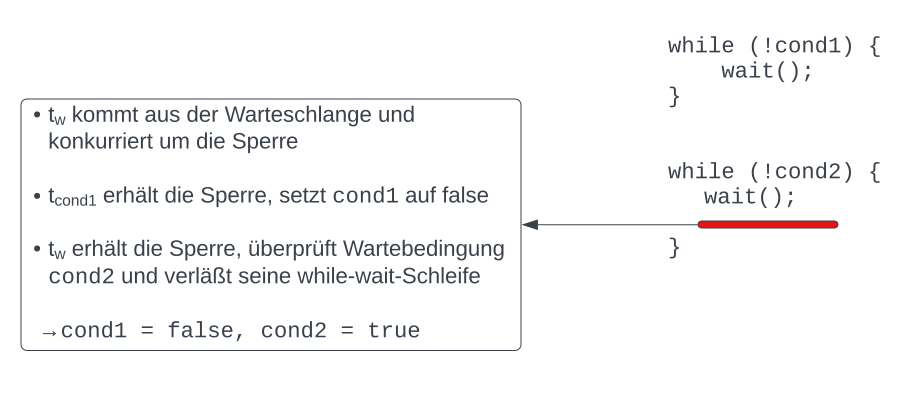
\includegraphics[scale=0.4]{chapters/Anhang/Klausuren/img/cond1cond2}
    \caption{in den rot markierten Bereich konkurriert $t_w$ um die Sperre des Objektes - wenn durch einen anderen Thread, der vor $t_w$ die Sperre erhält, \textit{cond1} auf \textit{false} gesetzt wird, stimmt die Ausgabe nicht mit der erwarteten überein. (Quelle: eigene)}
    \label{fig:cond1cond2}
\end{figure}

\noindent
Die korrekte Wartebedingung sollte lauten:

\begin{minted}[mathescape,
    linenos,
    numbersep=5pt,
    gobble=2,
    fontsize=\small,
    frame=lines,
    framesep=2mm]{java}
    public synchronized void cond1AndCond2() {
        while(!cond1 || !cond2) {
            try {
                wait();
            } catch(InterruptedException e) { }
        }
        System.out.println("cond1 and cond2:" + cond1 + " " + cond2);
    }
\end{minted}\\

Darüber hinaus müßte \code{notifyAll()} nur aufgerufen werden, wenn sowohl \code{cond1} als auch \code{cond2} auf \code{true} gesetzt sind, was leicht in den entsprechenden Methoden überprüft werden kann.
    \chapter{SS19}\label{ch:klausurss19}

\section{Aufgabe 1}

Bei der Aufgabe ist es wichtig, die Anforderungen genau zu beachten.\\
Ob eine Thread die while-wait-Schleife verlassen darf, wird von der Methode \code{tick()} gesteuert - wieviele Ticks ein Thread in der Schleife bleiben soll, wird von dem jeweiligen Thread definiert.\\
Die \code{tick()}-Methode wird von anderen Threads aufgerufen, es kann also durchaus vorkommen, dass mehrmals hintereinander
die \code{notifyAll()}-Methode aufgerufen wird - diese entfernt alle Threads aus der Warteschlange, damit die Threads ihre
Wartebedingungen erneut überprüfen können.\\
da \code{tick()} aber auch gleichzeitig einen Zähler realisieren soll, \textit{muss} es in der Methode auch eine Zählvariable geben, anhand derer die in der while-wait-Schleife enthaltenen Threads feststellen können, wie oft \code{tick()} aufgerufen wurde, um entsprechend aus der Schleife und nachfolgend der Methode herauszukommen.

\begin{figure}
    \centering
    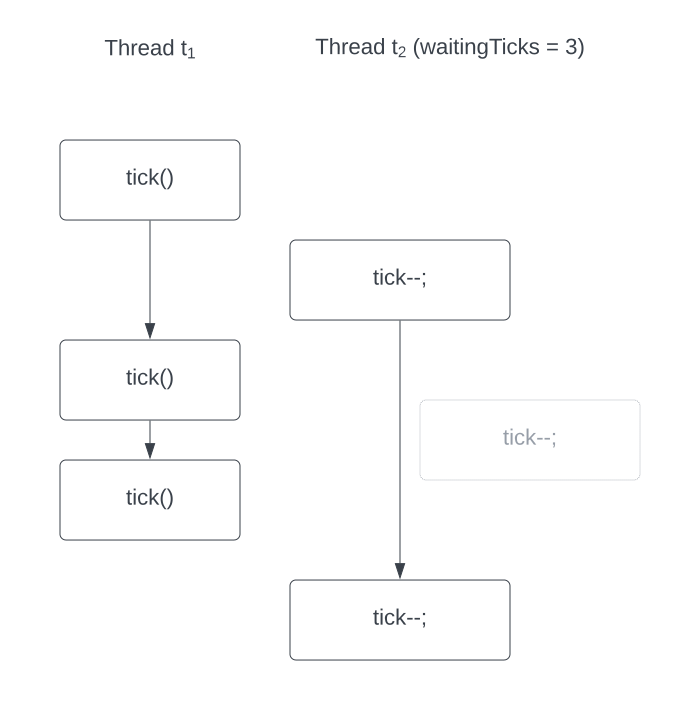
\includegraphics[scale=0.5]{chapters/Anhang/Klausuren/img/tick}
    \caption{Thread $t_1$ ruft 3 mal \texit{tick()} auf. Den Anforderungen nach müsste Thread $t_2$ danach aus der while-wait-Schleife herauskommen, erhält aber nicht die Sperre auf das Objekt von LogicalTime, um seinen eigenen Zähler rechtzeitig zu erniedrigen, bevor $t_1$ erneut \textit{tick()} aufruft. (Quelle: eigene)}
    \label{fig:tick}
\end{figure}

\section{Aufgabe 6}
Auch hier gilt, dass die Aufgabenstellung aufmerksam zu lesen ist.\\
Der Kreis soll erst ausgefüllt werden, wenn die Maustaste gelöst wird.

\begin{minted}[mathescape,
    linenos,
    numbersep=5pt,
    gobble=2,
    frame=lines,
    framesep=2mm]{java}
    private void mousePressed(double x, double y) {
        c = new Circle();
        c.setCenterX(x);
        c.setCenterY(y);
        c.setStroke(Color.RED);
        c.setFill(null); // oder Color.TRANSPARENT
        c.setRadius(RADIUS);
        graphicsPane.getChildren().add(c);
    }

    private void mouseReleased() {
        c.setFill(Color.RED);
        c = null;
    }
\end{minted}

\section{Aufgabe 8}

In der Abbildung \ref{fig:batchmodus} ist links der sequentielle Modus dargestellt, bei dem nach dem Senden einer Nachricht auf die Antwort des Servers gewartet wird, bevor eine neue Nachricht geschickt wird.
Dies wird i.d.R. verwendet, wenn das Senden einer neuen Nachricht abhängig ist von einem Ergebnis, die über die Server-Antwort übermittelt wird, oder wenn mit dem Server interagiert wird (Request abhängig vom Response).\\
Der Batch-Modus auf der rechten Seite der gleichen Abbildung ist schneller, da zwischen dem Senden von Nachrichten nicht auf Antworten gewartet werden müssen. \\
Erst nach dem Senden eine Batches von Nachrichten werden die dem Client zur Verfügung stehenden Antworten ausgelesen.\\

\noindent
In dieser Form des Batch-Modus besteht allerdings die Gefahr, dass es zu Verklemmungen kommt:
\begin{itemize}
    \item Bei dem Client kommen viele Nachrichten an, während er noch sendet.
    \item Die ankommenden Nachrichten für den Client werden gepuffert, bis sie ausgelesen werden (TCP- / OS-seitig).
    \item Läuft der Puffer voll, sorgt die Flusskontrolle (TCP) dafür, dass dem Sender mitgeteilt wird, dass keine Nachrichten mehr empfangen werden können, der Server sendet nicht mehr.
    \item Die zu sendenden Nachrichten des Servers werden in einen Puffer geschrieben.
    \item Der Sende-Puffer des Senders läuft voll.
    \item Bei dem nächsten Sende-Aufruf blockiert der Server, empfangene Nachrichten landen im Empfangspuffer
    \item Der Empfangspuffer des Servers läuft voll, der Client buffert die zu sendenden Nachrichten.
    \item Beide Anwendungen blockieren.
\end{itemize}

\\noindent
Um dieses Problem beim Batch-Modus zu umgehen, werden für das Senden und Empfangen zwei Threads auf Client-Seite erstellt: Ein Thread sendet, ein Thread empfängt. \\
Dadurch kann von dem Client immer wieder sein Empfangspuffer geleert werden, der Server wird beim Senden nicht blockiert.

\begin{figure}
    \centering
    \includegraphics[scale=0.4]{chapters/Anhang/Klausuren/img/batchmodus}
    \caption{Vereinfachte Darstellung sequentieller Kommunikation und Batch-Modus (Quelle: eigene)}
    \label{fig:batchmodus}
\end{figure}
    
\begin{appendices}
    
\begin{appendices}
    \input{chapters/Anhang/Zusatzaufgaben/index}
    \input{chapters/Anhang/Klausuren/ws13}
    \input{chapters/Anhang/Klausuren/ws15-16}
    \input{chapters/Anhang/Klausuren/ws16-17}
    \input{chapters/Anhang/Klausuren/ss19}
    \input{chapters/Anhang/Präsenzphase/index}

\end{appendices}

    \chapter{WS13}\label{ch:klausurws13}

\section{Aufgabe 1}
\subsection{Lösungsvorschlag}


\begin{minted}[mathescape,
    linenos,
    numbersep=5pt,
    gobble=2,
    fontsize=\small,
    frame=lines,
    framesep=2mm]{java}
    class Zahlenschloss {

        private int[] kombination;

        private int[] state;

        private boolean opened = false;

        public Zahlenschloss(int[] kombination) {
            this.kombination = kombination;
            this.state = new int[kombination.length];
        }

        public int anzahlRaedchen() {
            return kombination.length;
        }

        public synchronized int lesen(int radnummer) {
            return state[radnummer];
        }

        public synchronized void drehen(int radnummer, int zahl) {

            state[radnummer] = zahl;
            opened = true;
            for (int i = 0; i < anzahlRaedchen(); i++) {
                if (lesen(i) != kombination[i]) {
                    opened = false;
                    break;
                }
            }

            if (opened) {
                this.notify();
            }
        }

        public synchronized void warten() {

            while (!opened) {
                try {
                    this.wait();
                } catch (InterruptedException ignored) {}
            }
        }
    }
\end{minted}\\


\subsection{Anmerkung und Ergänzungen}

\begin{itemize}
    \item Es wird eine Wartebedingung benötigt, und zwar für die Methode \code{warten()}; ankommende Threads werden
    in die Warteschlange des Zahlenschloss-Objektes geschickt, wenn \code{opened} auf false gesetzt ist, ansonsten
    verlassen diese direkt die Methode wieder.\\
    Die Methode \code{drehen} benötigt keine separate Wartebedingung.
    Es reicht aus, sicherzustellen, dass das Zahlenschloss nicht gleichzeitig von anderen Threads benutzt werden kann:
    Die Methode \code{drehen} ist hierfür synchronisiert, damit das Zahlenschloss {insg.} immer nur eine Zustandsänderung
    erfährt - es sind andere Implementierungen möglich, in denen das Zahlenschloss dann von mehreren Threads gleichzeitig
    genutzt werden darf, wenn sich die Zugriffe anhand der ``Ziel``-\code{radnummer} unterscheiden, {bspw.} durch Mutex-Semaphore,
    die pro Radnummer verwendet werden\footnote{
        der gleichzeitige Zugriff auf unterschiedliche Arrays-Indizes ist erlaubt, s. `´17.4.1. Shared Variables``: \url{https://docs.oracle.com/javase/specs/jls/se21/html/jls-17.html#jls-1.4.1} - abgerufen 14.2.2024
    }.
    \item Es gibt nur eine Wartebedingung, von daher sollte \code{notify()} genügen.\\
    Wenn wir allerdings davon ausgehen, dass mehrere Threads über die Methode \code{warten()} in die Warteschlange des Objektes eingereiht worden sind,  sollte \code{notifyAll()} verwendet werden (siehe hierzu auch Abschnitt \ref{subsec:notifyAll}).
    Dennoch ist nicht garantiert, dass auch alle Threads aus der Warteschlange gelangen, denn es kann sein, dass ein anderer Thread die Methode \code{drehen()} betritt, dort die
    Zahlenkombination ändert und \code{opened} wieder auf \code{false} gesetzt wird. \\
    Ein anderer Thread, der nun in  \code{warten()} an die Reihe kommt, überprüft die Wartebedingung, und wird wieder in die Warteschlange eingereiht.
    Es ist also durchaus möglich, dass ein Thread nicht mehr aus der Methode \code{warten()} herauskommt.\\
    Dies könnte bspw. dadurch verhindert werden, dass die Threads in eine Queue gepackt werden, und in \code{drehen()} eine Wartebedingung eingefügt wird, die erst erfüllt ist,
    wenn die Queue geleert wurde oder aus ihr entnommen wurde, in der Reihenfolge, in der die Threads in die Queue eingereiht worden sind (\textit{FIFO}) (s. a. Abschnitt~\ref{subsec:readerwriterproblem}).
    \item Bei der Teilaufgabe mit der Schleife muss die komplette Schleife synchronisiert werden, was man durch ein \code{synchronized}-Statement erreicht\footnote{siehe Abschnitt~\ref{subsec:synchronizedstatement}.}
    \begin{minted}[mathescape,
        linenos,
        numbersep=5pt,
        gobble=2,
        fontsize=\small,
        frame=lines,
        framesep=2mm]{java}
        synchronized (zk) {
            for (int i = 0; i < anzahlRaedchen; i++) {
                System.out.println(zk.lesen(i));
            }
        }
    \end{minted}
    Ansonsten läuft man Gefahr, dass sich nach Auslesen der 1. Position der Wert von Position 2 geändert hat und dadurch eine
    Zahlenkombination ausgegeben wird, die es nicht gegeben hat:
    \begin{enumerate}
        \item $K\coloneqq[0, 0, 0]$
        \item Position $K_0$ wird ausgelesen und liefert $0$.
        \item Thread ändert $K_0$ zu $1$ $\implies K\coloneqq[1, 0, 0] $.
        \item Thread ändert $K_1$ zu $2$ $\implies K\coloneqq[1, 2, 0] $.
        \item Thread ändert $K_2$ zu $3$ $\implies K\coloneqq[1, 2, 3] $.
        \item Positionen $K_1$ und $K_2$ werden ausgelesen und liefern: $2, 3$
        \item Ausgabe: $0, 2, 3$ - diese Kombination hat es in dem Fall aber tatsächlich nicht gegeben.
    \end{enumerate}
\end{itemize}

\begin{tcolorbox}[colback=red!20,color=white,title=Anmerkung]
    Die Methode \code{lesen()} als \code{synchronized} zu markieren könnte man sich vlt. sparen, wenn man davon ausgeht,
    dass die Methode ohnehin in einem \code{synchronized}-Statement verwendet wird, um alle Rädchen abzulesen.\\
    Mehrere Threads können also nicht parallel auf unterschiedliche Positionen des Feldes zugreifen, wenn die Methode
    synchronisiert ist.\\
    Allerdings ist sowohl das Skript als auch das Buch recht klar, was in dieser Situation geschehen muss (s. Skript Fopt1/2, S. 9, außerdem \cite[31, Abschnitt 2.3.6]{Oec22}): Es muss (in diesem Kurs) immer \code{synchronized} verwendet werden, wenn gleichzeitig
    Daten geschrieben und gleichzeitig diese Daten gelesen werden sollen - und eine andere Implementierung, bei der die
    einzelnen Positionen ``gelocked`` sind, so dass ein gleichzeitiger Zugriff auf unterschiedliche Rädchen möglich ist, war nicht gefordert.\\
    Ggfl. würde in anderen Implementierungen der Einsatz von \code{AtomicReferenceArray}\footnote{s. \cite[157 ff.]{Oec22}
    s. ``Class AtomicReferenceArray<E>``: \url{https://docs.oracle.com/en/java/javase/21/docs/api/java.base/java/util/concurrent/atomic/AtomicReferenceArray.html} - abgerufen 15.2.2024
    } Sinn machen, aber das Lehrmaterial ist bereits sehr eindeutig bzgl. der Verwendung von \code{synchronized}.
\end{tcolorbox}



\section{Aufgabe 3}
\subsection{Lösungsvorschlag}

\subsection*{Statische Parallelität}
Statische Parallelität erlaubt es einem Server, eine \textit{fixe} Anzahl von Verbindungen gleichzeitig zu bedienen.\\
Hierbei wird ein Feld von Threads erstellt, wobei jeder Thread das \code{ServerSocket}-Objekt als Referenz übergeben bekommt.
In der \code{run()}-Methode wird dann über \code{accept()} in einer Endlosschleife auf eingehende Verbindungen gewartet, die dann so lange bedient werden, bis sich ein Client wieder abmeldet (oder eine andere Abbruchbedingung erfüllt ist, wie z.B. ein \code{SocketTimeout}).\\
Das sich ein Client abmeldet, bekommt man bspw. dadurch mit, dass \code{null} beim Lesen von einer Nachricht des Clients zurückgegeben wird (vgl. \cite[286]{Oec22}. \\
Siehe Abschnitt~\ref{sec:seqparserver} für ein Implementierungsbeispiel.



\subsection*{Dynamische Parallelität}

Bei der \textbf{Dynamischer Parallelität} erzeugt der Server für jede Verbindung einen neuen Thread, der so lange läuft, bis der Client die Verbindung wieder trennt.\\
Die Anzahl der Threads ändert sich dadurch laufend.\\
Wird die max. Anzahl erlaubter Threads nicht kontrolliert, kann es zu einer Überlastung des Server-Rechners kommen (bspw. durch einen Denial-of-Service-Angriff.)\\

\noindent
I.d.R. ist eine Mischform aus beidem geeignet, um mehrere Clients gleichzeitig bedienen zu können, und dabei nicht Gefahr zu laufen, durch dynamisches, unbegrenztes Wachstum der Anzahl der Threads überlastet zu werden.

    \chapter{WS13}\label{ch:klausurws5-16}

\section{Rechteck-Scroll (SS15 Aufgabe 2)}

Aufgabenstellung unklar.\\
Mögliche Implementierung unter \url{https://github.com/ThorstenSuckow/fopt/tree/main/src/main/java/klausurvorbereitung/foptws1516/MouseDragsSquareDemo}.

\section{Rechteck-Scroll (WS15/16 Aufgabe 1)}

Aufgabenstellung unklar.\\
Mögliche Implementierung unter \url{https://github.com/ThorstenSuckow/fopt/tree/main/src/main/java/klausurvorbereitung/foptws1516/MaxWeightDemo}.\\

\noindent
Es gibt nur eine Warteschlange für Threads in \code{use()}, es gibt keine Wartebedingung in \code{dontUse()} und damit auch keine weitere Warteschlange.\\
Es sind durch die Zugriffe auf unterschiedliche Indizes allerdings mehrere Wartebedingungen vorhanden, weshalb hab \code{notifyAll()} nutzen sollte,
sobald ein Zugriff auf ein Feld nach Aufruf von \code{dontUse} wieder möglich wird.\\
Ansonsten bestünde die Gefahr, dass bei dem Einsatz von \code{notify()} ein wartender Thread nicht geweckt wird, obwohl er weiterlaufen könnte:\\
Angenommen, das Feld $F$ hat eine Länge von $3$, das \code{maxWeight} ist mit $2$ konfiguriert.
Thread $t_1$ mit einer Laufzeit von $200\ sek$ bekommt Zugriff auf $F_0$, setzt $currentWeight$ auf $1$.\\
Thread $t_2$ mit einer Laufzeit von $1\ sek$ möchte auf $F_1$ zugreifen, setzt $currentWeight=2$ in die Warteschlange.\\
Thread $t_3$ meldet Zugriff auf $F_0$ an und gelangt in die Warteschlange.\\
Thread $t_4$ meldet Zugriff auf $F_1$ an und gelangt in die Warteschlange.\\
Thread $t_2$ ist mit der Bearbeitung von $F_1$ fertig, $currentWeight$ wird auf $1$ gesetzt, \code{notify()} wird aufgerufen.\\
Thread $t_3$ wird aus der Warteschlange geholt, kann aber nicht weiterarbeiten, da $F_0$ noch durch den länger dauernden $t_1$ blockiert ist, und kommt wieder in die Warteschlange.\\

\noindent
Offensichtlich hätte in dem Beispiel \code{notifyAll()} dazu geführt, dass auch $T_4$ seine Wartebedingung hätte überprüfen können, und hätte so Zugriff auf $F_1$ bekommen.
Stattdessen muss nun gewartet werden, bis das nächste \code{notify()} aufgerufen wird, oder ein neu ankommender Thread $F_1$ belegt.

    \chapter{WS16-17}\label{ch:klausurws16-17}

\section{Aufgabe 1}
\subsection{Lösungshinweis}

Die erste Aufgabe verdeutlicht, was bei einem \code{notifyAll()} und unsauber gesetzten Wartebedingungen passieren kann.\\
Sei folgender Quellcode gegeben:


\begin{minted}[mathescape,
    linenos,
    numbersep=5pt,
    gobble=2,
    fontsize=\small,
    frame=lines,
    framesep=2mm]{java}
    class Cond1AndCond2 {

        private boolean cond1;
        private boolean cond2;

        public synchronized void setCond1(boolean c) {
            cond1 = c;
            notifyAll();
        }

        public synchronized void setCond2(boolean c) {
            cond2 = c;
            notifyAll();
        }

        public synchronized void cond1AndCond2() {
            while(!cond1) {
                try {
                    wait();
                } catch(InterruptedException e) { }
            }

            while(!cond2) {
                try {
                    wait();
                } catch(InterruptedException e) {}
            }
            System.out.println("cond1 and cond2:" + cond1 + " " + cond2);
        }
    }
\end{minted}\\

Man sollte auf den ersten Blick meinen, dass \code{cond1} und \code{cond2} beide \code{true} sein müssen, damit die Ausgabe erfolgt.\\
Tatsächlich ist es aber so, dass es in der Methode zwei unterschiedliche Wartebedingungen gibt.\\
Die erste Wartebedingung schickt einen Thread in die Warteschlange, wenn \code{cond1 == false} gilt.\\
Setzt ein anderer Thread über \code{setCond1(true)} das Attribut entsprechend auf \code{true}, bewirkt der nachfolgende Aufruf von \code{notifyAll()}, dass alle \textit{wartenden} Threads aus der Warteschlange entfernt werden und erneut um eine Sperre des Objektes konkurrieren.\\
Erhält ein entsprechender Thread $t_w$ die Sperre auf das Objekt und kann seine \textit{while-wait-Schleife} verlassen, kann es vorkommen, dass er erneut in die Warteschlange eingereiht wird, wegen der nachfolgenden Wartebedingung \code{cond2 == false}.\\
Angenommen, ein weiterer Thread ruft nun \code{setCond2(true)} auf, und $t_w$ kommt aus der Warteschlange und konkurriert erneut und um die Sperre des Objektes, dann kann es vorkommen, das ein anderer Thread zunächst die Sperre erhält, \code{cond1} wieder auf \code{false} setzt, dann erhält $t_w$ die Sperre, überprüft die Wartebedingung \code{cond2 == false}.\\
Wegen \code{cond2} gelangt er aus der \textit{while-wait-Schleife} und die Ausgabe erfolgt - da zwischenzeitlich \code{cond1} wieder auf \code{false} gesetzt wurde, ist die erwartete Ausgabe nicht \code{true true}, sondern \code{false true} (s. Abbildung \ref{fig:cond1cond2}).\\

\begin{figure}
    \centering
    \includegraphics[scale=0.4]{chapters/Anhang/Klausuren/img/cond1cond2}
    \caption{in den rot markierten Bereich konkurriert $t_w$ um die Sperre des Objektes - wenn durch einen anderen Thread, der vor $t_w$ die Sperre erhält, \textit{cond1} auf \textit{false} gesetzt wird, stimmt die Ausgabe nicht mit der erwarteten überein. (Quelle: eigene)}
    \label{fig:cond1cond2}
\end{figure}

\noindent
Die korrekte Wartebedingung sollte lauten:

\begin{minted}[mathescape,
    linenos,
    numbersep=5pt,
    gobble=2,
    fontsize=\small,
    frame=lines,
    framesep=2mm]{java}
    public synchronized void cond1AndCond2() {
        while(!cond1 || !cond2) {
            try {
                wait();
            } catch(InterruptedException e) { }
        }
        System.out.println("cond1 and cond2:" + cond1 + " " + cond2);
    }
\end{minted}\\

Darüber hinaus müßte \code{notifyAll()} nur aufgerufen werden, wenn sowohl \code{cond1} als auch \code{cond2} auf \code{true} gesetzt sind, was leicht in den entsprechenden Methoden überprüft werden kann.
    \chapter{SS19}\label{ch:klausurss19}

\section{Aufgabe 1}

Bei der Aufgabe ist es wichtig, die Anforderungen genau zu beachten.\\
Ob eine Thread die while-wait-Schleife verlassen darf, wird von der Methode \code{tick()} gesteuert - wieviele Ticks ein Thread in der Schleife bleiben soll, wird von dem jeweiligen Thread definiert.\\
Die \code{tick()}-Methode wird von anderen Threads aufgerufen, es kann also durchaus vorkommen, dass mehrmals hintereinander
die \code{notifyAll()}-Methode aufgerufen wird - diese entfernt alle Threads aus der Warteschlange, damit die Threads ihre
Wartebedingungen erneut überprüfen können.\\
da \code{tick()} aber auch gleichzeitig einen Zähler realisieren soll, \textit{muss} es in der Methode auch eine Zählvariable geben, anhand derer die in der while-wait-Schleife enthaltenen Threads feststellen können, wie oft \code{tick()} aufgerufen wurde, um entsprechend aus der Schleife und nachfolgend der Methode herauszukommen.

\begin{figure}
    \centering
    \includegraphics[scale=0.5]{chapters/Anhang/Klausuren/img/tick}
    \caption{Thread $t_1$ ruft 3 mal \texit{tick()} auf. Den Anforderungen nach müsste Thread $t_2$ danach aus der while-wait-Schleife herauskommen, erhält aber nicht die Sperre auf das Objekt von LogicalTime, um seinen eigenen Zähler rechtzeitig zu erniedrigen, bevor $t_1$ erneut \textit{tick()} aufruft. (Quelle: eigene)}
    \label{fig:tick}
\end{figure}

\section{Aufgabe 6}
Auch hier gilt, dass die Aufgabenstellung aufmerksam zu lesen ist.\\
Der Kreis soll erst ausgefüllt werden, wenn die Maustaste gelöst wird.

\begin{minted}[mathescape,
    linenos,
    numbersep=5pt,
    gobble=2,
    frame=lines,
    framesep=2mm]{java}
    private void mousePressed(double x, double y) {
        c = new Circle();
        c.setCenterX(x);
        c.setCenterY(y);
        c.setStroke(Color.RED);
        c.setFill(null); // oder Color.TRANSPARENT
        c.setRadius(RADIUS);
        graphicsPane.getChildren().add(c);
    }

    private void mouseReleased() {
        c.setFill(Color.RED);
        c = null;
    }
\end{minted}

\section{Aufgabe 8}

In der Abbildung \ref{fig:batchmodus} ist links der sequentielle Modus dargestellt, bei dem nach dem Senden einer Nachricht auf die Antwort des Servers gewartet wird, bevor eine neue Nachricht geschickt wird.
Dies wird i.d.R. verwendet, wenn das Senden einer neuen Nachricht abhängig ist von einem Ergebnis, die über die Server-Antwort übermittelt wird, oder wenn mit dem Server interagiert wird (Request abhängig vom Response).\\
Der Batch-Modus auf der rechten Seite der gleichen Abbildung ist schneller, da zwischen dem Senden von Nachrichten nicht auf Antworten gewartet werden müssen. \\
Erst nach dem Senden eine Batches von Nachrichten werden die dem Client zur Verfügung stehenden Antworten ausgelesen.\\

\noindent
In dieser Form des Batch-Modus besteht allerdings die Gefahr, dass es zu Verklemmungen kommt:
\begin{itemize}
    \item Bei dem Client kommen viele Nachrichten an, während er noch sendet.
    \item Die ankommenden Nachrichten für den Client werden gepuffert, bis sie ausgelesen werden (TCP- / OS-seitig).
    \item Läuft der Puffer voll, sorgt die Flusskontrolle (TCP) dafür, dass dem Sender mitgeteilt wird, dass keine Nachrichten mehr empfangen werden können, der Server sendet nicht mehr.
    \item Die zu sendenden Nachrichten des Servers werden in einen Puffer geschrieben.
    \item Der Sende-Puffer des Senders läuft voll.
    \item Bei dem nächsten Sende-Aufruf blockiert der Server, empfangene Nachrichten landen im Empfangspuffer
    \item Der Empfangspuffer des Servers läuft voll, der Client buffert die zu sendenden Nachrichten.
    \item Beide Anwendungen blockieren.
\end{itemize}

\\noindent
Um dieses Problem beim Batch-Modus zu umgehen, werden für das Senden und Empfangen zwei Threads auf Client-Seite erstellt: Ein Thread sendet, ein Thread empfängt. \\
Dadurch kann von dem Client immer wieder sein Empfangspuffer geleert werden, der Server wird beim Senden nicht blockiert.

\begin{figure}
    \centering
    \includegraphics[scale=0.4]{chapters/Anhang/Klausuren/img/batchmodus}
    \caption{Vereinfachte Darstellung sequentieller Kommunikation und Batch-Modus (Quelle: eigene)}
    \label{fig:batchmodus}
\end{figure}
    
\begin{appendices}
    \input{chapters/Anhang/Zusatzaufgaben/index}
    \input{chapters/Anhang/Klausuren/ws13}
    \input{chapters/Anhang/Klausuren/ws15-16}
    \input{chapters/Anhang/Klausuren/ws16-17}
    \input{chapters/Anhang/Klausuren/ss19}
    \input{chapters/Anhang/Präsenzphase/index}

\end{appendices}


\end{appendices}


\end{appendices}



\begin{appendices}
    
\begin{appendices}
    
\begin{appendices}
    \input{chapters/Anhang/Zusatzaufgaben/index}
    \input{chapters/Anhang/Klausuren/ws13}
    \input{chapters/Anhang/Klausuren/ws15-16}
    \input{chapters/Anhang/Klausuren/ws16-17}
    \input{chapters/Anhang/Klausuren/ss19}
    \input{chapters/Anhang/Präsenzphase/index}

\end{appendices}

    \chapter{WS13}\label{ch:klausurws13}

\section{Aufgabe 1}
\subsection{Lösungsvorschlag}


\begin{minted}[mathescape,
    linenos,
    numbersep=5pt,
    gobble=2,
    fontsize=\small,
    frame=lines,
    framesep=2mm]{java}
    class Zahlenschloss {

        private int[] kombination;

        private int[] state;

        private boolean opened = false;

        public Zahlenschloss(int[] kombination) {
            this.kombination = kombination;
            this.state = new int[kombination.length];
        }

        public int anzahlRaedchen() {
            return kombination.length;
        }

        public synchronized int lesen(int radnummer) {
            return state[radnummer];
        }

        public synchronized void drehen(int radnummer, int zahl) {

            state[radnummer] = zahl;
            opened = true;
            for (int i = 0; i < anzahlRaedchen(); i++) {
                if (lesen(i) != kombination[i]) {
                    opened = false;
                    break;
                }
            }

            if (opened) {
                this.notify();
            }
        }

        public synchronized void warten() {

            while (!opened) {
                try {
                    this.wait();
                } catch (InterruptedException ignored) {}
            }
        }
    }
\end{minted}\\


\subsection{Anmerkung und Ergänzungen}

\begin{itemize}
    \item Es wird eine Wartebedingung benötigt, und zwar für die Methode \code{warten()}; ankommende Threads werden
    in die Warteschlange des Zahlenschloss-Objektes geschickt, wenn \code{opened} auf false gesetzt ist, ansonsten
    verlassen diese direkt die Methode wieder.\\
    Die Methode \code{drehen} benötigt keine separate Wartebedingung.
    Es reicht aus, sicherzustellen, dass das Zahlenschloss nicht gleichzeitig von anderen Threads benutzt werden kann:
    Die Methode \code{drehen} ist hierfür synchronisiert, damit das Zahlenschloss {insg.} immer nur eine Zustandsänderung
    erfährt - es sind andere Implementierungen möglich, in denen das Zahlenschloss dann von mehreren Threads gleichzeitig
    genutzt werden darf, wenn sich die Zugriffe anhand der ``Ziel``-\code{radnummer} unterscheiden, {bspw.} durch Mutex-Semaphore,
    die pro Radnummer verwendet werden\footnote{
        der gleichzeitige Zugriff auf unterschiedliche Arrays-Indizes ist erlaubt, s. `´17.4.1. Shared Variables``: \url{https://docs.oracle.com/javase/specs/jls/se21/html/jls-17.html#jls-1.4.1} - abgerufen 14.2.2024
    }.
    \item Es gibt nur eine Wartebedingung, von daher sollte \code{notify()} genügen.\\
    Wenn wir allerdings davon ausgehen, dass mehrere Threads über die Methode \code{warten()} in die Warteschlange des Objektes eingereiht worden sind,  sollte \code{notifyAll()} verwendet werden (siehe hierzu auch Abschnitt \ref{subsec:notifyAll}).
    Dennoch ist nicht garantiert, dass auch alle Threads aus der Warteschlange gelangen, denn es kann sein, dass ein anderer Thread die Methode \code{drehen()} betritt, dort die
    Zahlenkombination ändert und \code{opened} wieder auf \code{false} gesetzt wird. \\
    Ein anderer Thread, der nun in  \code{warten()} an die Reihe kommt, überprüft die Wartebedingung, und wird wieder in die Warteschlange eingereiht.
    Es ist also durchaus möglich, dass ein Thread nicht mehr aus der Methode \code{warten()} herauskommt.\\
    Dies könnte bspw. dadurch verhindert werden, dass die Threads in eine Queue gepackt werden, und in \code{drehen()} eine Wartebedingung eingefügt wird, die erst erfüllt ist,
    wenn die Queue geleert wurde oder aus ihr entnommen wurde, in der Reihenfolge, in der die Threads in die Queue eingereiht worden sind (\textit{FIFO}) (s. a. Abschnitt~\ref{subsec:readerwriterproblem}).
    \item Bei der Teilaufgabe mit der Schleife muss die komplette Schleife synchronisiert werden, was man durch ein \code{synchronized}-Statement erreicht\footnote{siehe Abschnitt~\ref{subsec:synchronizedstatement}.}
    \begin{minted}[mathescape,
        linenos,
        numbersep=5pt,
        gobble=2,
        fontsize=\small,
        frame=lines,
        framesep=2mm]{java}
        synchronized (zk) {
            for (int i = 0; i < anzahlRaedchen; i++) {
                System.out.println(zk.lesen(i));
            }
        }
    \end{minted}
    Ansonsten läuft man Gefahr, dass sich nach Auslesen der 1. Position der Wert von Position 2 geändert hat und dadurch eine
    Zahlenkombination ausgegeben wird, die es nicht gegeben hat:
    \begin{enumerate}
        \item $K\coloneqq[0, 0, 0]$
        \item Position $K_0$ wird ausgelesen und liefert $0$.
        \item Thread ändert $K_0$ zu $1$ $\implies K\coloneqq[1, 0, 0] $.
        \item Thread ändert $K_1$ zu $2$ $\implies K\coloneqq[1, 2, 0] $.
        \item Thread ändert $K_2$ zu $3$ $\implies K\coloneqq[1, 2, 3] $.
        \item Positionen $K_1$ und $K_2$ werden ausgelesen und liefern: $2, 3$
        \item Ausgabe: $0, 2, 3$ - diese Kombination hat es in dem Fall aber tatsächlich nicht gegeben.
    \end{enumerate}
\end{itemize}

\begin{tcolorbox}[colback=red!20,color=white,title=Anmerkung]
    Die Methode \code{lesen()} als \code{synchronized} zu markieren könnte man sich vlt. sparen, wenn man davon ausgeht,
    dass die Methode ohnehin in einem \code{synchronized}-Statement verwendet wird, um alle Rädchen abzulesen.\\
    Mehrere Threads können also nicht parallel auf unterschiedliche Positionen des Feldes zugreifen, wenn die Methode
    synchronisiert ist.\\
    Allerdings ist sowohl das Skript als auch das Buch recht klar, was in dieser Situation geschehen muss (s. Skript Fopt1/2, S. 9, außerdem \cite[31, Abschnitt 2.3.6]{Oec22}): Es muss (in diesem Kurs) immer \code{synchronized} verwendet werden, wenn gleichzeitig
    Daten geschrieben und gleichzeitig diese Daten gelesen werden sollen - und eine andere Implementierung, bei der die
    einzelnen Positionen ``gelocked`` sind, so dass ein gleichzeitiger Zugriff auf unterschiedliche Rädchen möglich ist, war nicht gefordert.\\
    Ggfl. würde in anderen Implementierungen der Einsatz von \code{AtomicReferenceArray}\footnote{s. \cite[157 ff.]{Oec22}
    s. ``Class AtomicReferenceArray<E>``: \url{https://docs.oracle.com/en/java/javase/21/docs/api/java.base/java/util/concurrent/atomic/AtomicReferenceArray.html} - abgerufen 15.2.2024
    } Sinn machen, aber das Lehrmaterial ist bereits sehr eindeutig bzgl. der Verwendung von \code{synchronized}.
\end{tcolorbox}



\section{Aufgabe 3}
\subsection{Lösungsvorschlag}

\subsection*{Statische Parallelität}
Statische Parallelität erlaubt es einem Server, eine \textit{fixe} Anzahl von Verbindungen gleichzeitig zu bedienen.\\
Hierbei wird ein Feld von Threads erstellt, wobei jeder Thread das \code{ServerSocket}-Objekt als Referenz übergeben bekommt.
In der \code{run()}-Methode wird dann über \code{accept()} in einer Endlosschleife auf eingehende Verbindungen gewartet, die dann so lange bedient werden, bis sich ein Client wieder abmeldet (oder eine andere Abbruchbedingung erfüllt ist, wie z.B. ein \code{SocketTimeout}).\\
Das sich ein Client abmeldet, bekommt man bspw. dadurch mit, dass \code{null} beim Lesen von einer Nachricht des Clients zurückgegeben wird (vgl. \cite[286]{Oec22}. \\
Siehe Abschnitt~\ref{sec:seqparserver} für ein Implementierungsbeispiel.



\subsection*{Dynamische Parallelität}

Bei der \textbf{Dynamischer Parallelität} erzeugt der Server für jede Verbindung einen neuen Thread, der so lange läuft, bis der Client die Verbindung wieder trennt.\\
Die Anzahl der Threads ändert sich dadurch laufend.\\
Wird die max. Anzahl erlaubter Threads nicht kontrolliert, kann es zu einer Überlastung des Server-Rechners kommen (bspw. durch einen Denial-of-Service-Angriff.)\\

\noindent
I.d.R. ist eine Mischform aus beidem geeignet, um mehrere Clients gleichzeitig bedienen zu können, und dabei nicht Gefahr zu laufen, durch dynamisches, unbegrenztes Wachstum der Anzahl der Threads überlastet zu werden.

    \chapter{WS13}\label{ch:klausurws5-16}

\section{Rechteck-Scroll (SS15 Aufgabe 2)}

Aufgabenstellung unklar.\\
Mögliche Implementierung unter \url{https://github.com/ThorstenSuckow/fopt/tree/main/src/main/java/klausurvorbereitung/foptws1516/MouseDragsSquareDemo}.

\section{Rechteck-Scroll (WS15/16 Aufgabe 1)}

Aufgabenstellung unklar.\\
Mögliche Implementierung unter \url{https://github.com/ThorstenSuckow/fopt/tree/main/src/main/java/klausurvorbereitung/foptws1516/MaxWeightDemo}.\\

\noindent
Es gibt nur eine Warteschlange für Threads in \code{use()}, es gibt keine Wartebedingung in \code{dontUse()} und damit auch keine weitere Warteschlange.\\
Es sind durch die Zugriffe auf unterschiedliche Indizes allerdings mehrere Wartebedingungen vorhanden, weshalb hab \code{notifyAll()} nutzen sollte,
sobald ein Zugriff auf ein Feld nach Aufruf von \code{dontUse} wieder möglich wird.\\
Ansonsten bestünde die Gefahr, dass bei dem Einsatz von \code{notify()} ein wartender Thread nicht geweckt wird, obwohl er weiterlaufen könnte:\\
Angenommen, das Feld $F$ hat eine Länge von $3$, das \code{maxWeight} ist mit $2$ konfiguriert.
Thread $t_1$ mit einer Laufzeit von $200\ sek$ bekommt Zugriff auf $F_0$, setzt $currentWeight$ auf $1$.\\
Thread $t_2$ mit einer Laufzeit von $1\ sek$ möchte auf $F_1$ zugreifen, setzt $currentWeight=2$ in die Warteschlange.\\
Thread $t_3$ meldet Zugriff auf $F_0$ an und gelangt in die Warteschlange.\\
Thread $t_4$ meldet Zugriff auf $F_1$ an und gelangt in die Warteschlange.\\
Thread $t_2$ ist mit der Bearbeitung von $F_1$ fertig, $currentWeight$ wird auf $1$ gesetzt, \code{notify()} wird aufgerufen.\\
Thread $t_3$ wird aus der Warteschlange geholt, kann aber nicht weiterarbeiten, da $F_0$ noch durch den länger dauernden $t_1$ blockiert ist, und kommt wieder in die Warteschlange.\\

\noindent
Offensichtlich hätte in dem Beispiel \code{notifyAll()} dazu geführt, dass auch $T_4$ seine Wartebedingung hätte überprüfen können, und hätte so Zugriff auf $F_1$ bekommen.
Stattdessen muss nun gewartet werden, bis das nächste \code{notify()} aufgerufen wird, oder ein neu ankommender Thread $F_1$ belegt.

    \chapter{WS16-17}\label{ch:klausurws16-17}

\section{Aufgabe 1}
\subsection{Lösungshinweis}

Die erste Aufgabe verdeutlicht, was bei einem \code{notifyAll()} und unsauber gesetzten Wartebedingungen passieren kann.\\
Sei folgender Quellcode gegeben:


\begin{minted}[mathescape,
    linenos,
    numbersep=5pt,
    gobble=2,
    fontsize=\small,
    frame=lines,
    framesep=2mm]{java}
    class Cond1AndCond2 {

        private boolean cond1;
        private boolean cond2;

        public synchronized void setCond1(boolean c) {
            cond1 = c;
            notifyAll();
        }

        public synchronized void setCond2(boolean c) {
            cond2 = c;
            notifyAll();
        }

        public synchronized void cond1AndCond2() {
            while(!cond1) {
                try {
                    wait();
                } catch(InterruptedException e) { }
            }

            while(!cond2) {
                try {
                    wait();
                } catch(InterruptedException e) {}
            }
            System.out.println("cond1 and cond2:" + cond1 + " " + cond2);
        }
    }
\end{minted}\\

Man sollte auf den ersten Blick meinen, dass \code{cond1} und \code{cond2} beide \code{true} sein müssen, damit die Ausgabe erfolgt.\\
Tatsächlich ist es aber so, dass es in der Methode zwei unterschiedliche Wartebedingungen gibt.\\
Die erste Wartebedingung schickt einen Thread in die Warteschlange, wenn \code{cond1 == false} gilt.\\
Setzt ein anderer Thread über \code{setCond1(true)} das Attribut entsprechend auf \code{true}, bewirkt der nachfolgende Aufruf von \code{notifyAll()}, dass alle \textit{wartenden} Threads aus der Warteschlange entfernt werden und erneut um eine Sperre des Objektes konkurrieren.\\
Erhält ein entsprechender Thread $t_w$ die Sperre auf das Objekt und kann seine \textit{while-wait-Schleife} verlassen, kann es vorkommen, dass er erneut in die Warteschlange eingereiht wird, wegen der nachfolgenden Wartebedingung \code{cond2 == false}.\\
Angenommen, ein weiterer Thread ruft nun \code{setCond2(true)} auf, und $t_w$ kommt aus der Warteschlange und konkurriert erneut und um die Sperre des Objektes, dann kann es vorkommen, das ein anderer Thread zunächst die Sperre erhält, \code{cond1} wieder auf \code{false} setzt, dann erhält $t_w$ die Sperre, überprüft die Wartebedingung \code{cond2 == false}.\\
Wegen \code{cond2} gelangt er aus der \textit{while-wait-Schleife} und die Ausgabe erfolgt - da zwischenzeitlich \code{cond1} wieder auf \code{false} gesetzt wurde, ist die erwartete Ausgabe nicht \code{true true}, sondern \code{false true} (s. Abbildung \ref{fig:cond1cond2}).\\

\begin{figure}
    \centering
    \includegraphics[scale=0.4]{chapters/Anhang/Klausuren/img/cond1cond2}
    \caption{in den rot markierten Bereich konkurriert $t_w$ um die Sperre des Objektes - wenn durch einen anderen Thread, der vor $t_w$ die Sperre erhält, \textit{cond1} auf \textit{false} gesetzt wird, stimmt die Ausgabe nicht mit der erwarteten überein. (Quelle: eigene)}
    \label{fig:cond1cond2}
\end{figure}

\noindent
Die korrekte Wartebedingung sollte lauten:

\begin{minted}[mathescape,
    linenos,
    numbersep=5pt,
    gobble=2,
    fontsize=\small,
    frame=lines,
    framesep=2mm]{java}
    public synchronized void cond1AndCond2() {
        while(!cond1 || !cond2) {
            try {
                wait();
            } catch(InterruptedException e) { }
        }
        System.out.println("cond1 and cond2:" + cond1 + " " + cond2);
    }
\end{minted}\\

Darüber hinaus müßte \code{notifyAll()} nur aufgerufen werden, wenn sowohl \code{cond1} als auch \code{cond2} auf \code{true} gesetzt sind, was leicht in den entsprechenden Methoden überprüft werden kann.
    \chapter{SS19}\label{ch:klausurss19}

\section{Aufgabe 1}

Bei der Aufgabe ist es wichtig, die Anforderungen genau zu beachten.\\
Ob eine Thread die while-wait-Schleife verlassen darf, wird von der Methode \code{tick()} gesteuert - wieviele Ticks ein Thread in der Schleife bleiben soll, wird von dem jeweiligen Thread definiert.\\
Die \code{tick()}-Methode wird von anderen Threads aufgerufen, es kann also durchaus vorkommen, dass mehrmals hintereinander
die \code{notifyAll()}-Methode aufgerufen wird - diese entfernt alle Threads aus der Warteschlange, damit die Threads ihre
Wartebedingungen erneut überprüfen können.\\
da \code{tick()} aber auch gleichzeitig einen Zähler realisieren soll, \textit{muss} es in der Methode auch eine Zählvariable geben, anhand derer die in der while-wait-Schleife enthaltenen Threads feststellen können, wie oft \code{tick()} aufgerufen wurde, um entsprechend aus der Schleife und nachfolgend der Methode herauszukommen.

\begin{figure}
    \centering
    \includegraphics[scale=0.5]{chapters/Anhang/Klausuren/img/tick}
    \caption{Thread $t_1$ ruft 3 mal \texit{tick()} auf. Den Anforderungen nach müsste Thread $t_2$ danach aus der while-wait-Schleife herauskommen, erhält aber nicht die Sperre auf das Objekt von LogicalTime, um seinen eigenen Zähler rechtzeitig zu erniedrigen, bevor $t_1$ erneut \textit{tick()} aufruft. (Quelle: eigene)}
    \label{fig:tick}
\end{figure}

\section{Aufgabe 6}
Auch hier gilt, dass die Aufgabenstellung aufmerksam zu lesen ist.\\
Der Kreis soll erst ausgefüllt werden, wenn die Maustaste gelöst wird.

\begin{minted}[mathescape,
    linenos,
    numbersep=5pt,
    gobble=2,
    frame=lines,
    framesep=2mm]{java}
    private void mousePressed(double x, double y) {
        c = new Circle();
        c.setCenterX(x);
        c.setCenterY(y);
        c.setStroke(Color.RED);
        c.setFill(null); // oder Color.TRANSPARENT
        c.setRadius(RADIUS);
        graphicsPane.getChildren().add(c);
    }

    private void mouseReleased() {
        c.setFill(Color.RED);
        c = null;
    }
\end{minted}

\section{Aufgabe 8}

In der Abbildung \ref{fig:batchmodus} ist links der sequentielle Modus dargestellt, bei dem nach dem Senden einer Nachricht auf die Antwort des Servers gewartet wird, bevor eine neue Nachricht geschickt wird.
Dies wird i.d.R. verwendet, wenn das Senden einer neuen Nachricht abhängig ist von einem Ergebnis, die über die Server-Antwort übermittelt wird, oder wenn mit dem Server interagiert wird (Request abhängig vom Response).\\
Der Batch-Modus auf der rechten Seite der gleichen Abbildung ist schneller, da zwischen dem Senden von Nachrichten nicht auf Antworten gewartet werden müssen. \\
Erst nach dem Senden eine Batches von Nachrichten werden die dem Client zur Verfügung stehenden Antworten ausgelesen.\\

\noindent
In dieser Form des Batch-Modus besteht allerdings die Gefahr, dass es zu Verklemmungen kommt:
\begin{itemize}
    \item Bei dem Client kommen viele Nachrichten an, während er noch sendet.
    \item Die ankommenden Nachrichten für den Client werden gepuffert, bis sie ausgelesen werden (TCP- / OS-seitig).
    \item Läuft der Puffer voll, sorgt die Flusskontrolle (TCP) dafür, dass dem Sender mitgeteilt wird, dass keine Nachrichten mehr empfangen werden können, der Server sendet nicht mehr.
    \item Die zu sendenden Nachrichten des Servers werden in einen Puffer geschrieben.
    \item Der Sende-Puffer des Senders läuft voll.
    \item Bei dem nächsten Sende-Aufruf blockiert der Server, empfangene Nachrichten landen im Empfangspuffer
    \item Der Empfangspuffer des Servers läuft voll, der Client buffert die zu sendenden Nachrichten.
    \item Beide Anwendungen blockieren.
\end{itemize}

\\noindent
Um dieses Problem beim Batch-Modus zu umgehen, werden für das Senden und Empfangen zwei Threads auf Client-Seite erstellt: Ein Thread sendet, ein Thread empfängt. \\
Dadurch kann von dem Client immer wieder sein Empfangspuffer geleert werden, der Server wird beim Senden nicht blockiert.

\begin{figure}
    \centering
    \includegraphics[scale=0.4]{chapters/Anhang/Klausuren/img/batchmodus}
    \caption{Vereinfachte Darstellung sequentieller Kommunikation und Batch-Modus (Quelle: eigene)}
    \label{fig:batchmodus}
\end{figure}
    
\begin{appendices}
    \input{chapters/Anhang/Zusatzaufgaben/index}
    \input{chapters/Anhang/Klausuren/ws13}
    \input{chapters/Anhang/Klausuren/ws15-16}
    \input{chapters/Anhang/Klausuren/ws16-17}
    \input{chapters/Anhang/Klausuren/ss19}
    \input{chapters/Anhang/Präsenzphase/index}

\end{appendices}


\end{appendices}

    \chapter{WS13}\label{ch:klausurws13}

\section{Aufgabe 1}
\subsection{Lösungsvorschlag}


\begin{minted}[mathescape,
    linenos,
    numbersep=5pt,
    gobble=2,
    fontsize=\small,
    frame=lines,
    framesep=2mm]{java}
    class Zahlenschloss {

        private int[] kombination;

        private int[] state;

        private boolean opened = false;

        public Zahlenschloss(int[] kombination) {
            this.kombination = kombination;
            this.state = new int[kombination.length];
        }

        public int anzahlRaedchen() {
            return kombination.length;
        }

        public synchronized int lesen(int radnummer) {
            return state[radnummer];
        }

        public synchronized void drehen(int radnummer, int zahl) {

            state[radnummer] = zahl;
            opened = true;
            for (int i = 0; i < anzahlRaedchen(); i++) {
                if (lesen(i) != kombination[i]) {
                    opened = false;
                    break;
                }
            }

            if (opened) {
                this.notify();
            }
        }

        public synchronized void warten() {

            while (!opened) {
                try {
                    this.wait();
                } catch (InterruptedException ignored) {}
            }
        }
    }
\end{minted}\\


\subsection{Anmerkung und Ergänzungen}

\begin{itemize}
    \item Es wird eine Wartebedingung benötigt, und zwar für die Methode \code{warten()}; ankommende Threads werden
    in die Warteschlange des Zahlenschloss-Objektes geschickt, wenn \code{opened} auf false gesetzt ist, ansonsten
    verlassen diese direkt die Methode wieder.\\
    Die Methode \code{drehen} benötigt keine separate Wartebedingung.
    Es reicht aus, sicherzustellen, dass das Zahlenschloss nicht gleichzeitig von anderen Threads benutzt werden kann:
    Die Methode \code{drehen} ist hierfür synchronisiert, damit das Zahlenschloss {insg.} immer nur eine Zustandsänderung
    erfährt - es sind andere Implementierungen möglich, in denen das Zahlenschloss dann von mehreren Threads gleichzeitig
    genutzt werden darf, wenn sich die Zugriffe anhand der ``Ziel``-\code{radnummer} unterscheiden, {bspw.} durch Mutex-Semaphore,
    die pro Radnummer verwendet werden\footnote{
        der gleichzeitige Zugriff auf unterschiedliche Arrays-Indizes ist erlaubt, s. `´17.4.1. Shared Variables``: \url{https://docs.oracle.com/javase/specs/jls/se21/html/jls-17.html#jls-1.4.1} - abgerufen 14.2.2024
    }.
    \item Es gibt nur eine Wartebedingung, von daher sollte \code{notify()} genügen.\\
    Wenn wir allerdings davon ausgehen, dass mehrere Threads über die Methode \code{warten()} in die Warteschlange des Objektes eingereiht worden sind,  sollte \code{notifyAll()} verwendet werden (siehe hierzu auch Abschnitt \ref{subsec:notifyAll}).
    Dennoch ist nicht garantiert, dass auch alle Threads aus der Warteschlange gelangen, denn es kann sein, dass ein anderer Thread die Methode \code{drehen()} betritt, dort die
    Zahlenkombination ändert und \code{opened} wieder auf \code{false} gesetzt wird. \\
    Ein anderer Thread, der nun in  \code{warten()} an die Reihe kommt, überprüft die Wartebedingung, und wird wieder in die Warteschlange eingereiht.
    Es ist also durchaus möglich, dass ein Thread nicht mehr aus der Methode \code{warten()} herauskommt.\\
    Dies könnte bspw. dadurch verhindert werden, dass die Threads in eine Queue gepackt werden, und in \code{drehen()} eine Wartebedingung eingefügt wird, die erst erfüllt ist,
    wenn die Queue geleert wurde oder aus ihr entnommen wurde, in der Reihenfolge, in der die Threads in die Queue eingereiht worden sind (\textit{FIFO}) (s. a. Abschnitt~\ref{subsec:readerwriterproblem}).
    \item Bei der Teilaufgabe mit der Schleife muss die komplette Schleife synchronisiert werden, was man durch ein \code{synchronized}-Statement erreicht\footnote{siehe Abschnitt~\ref{subsec:synchronizedstatement}.}
    \begin{minted}[mathescape,
        linenos,
        numbersep=5pt,
        gobble=2,
        fontsize=\small,
        frame=lines,
        framesep=2mm]{java}
        synchronized (zk) {
            for (int i = 0; i < anzahlRaedchen; i++) {
                System.out.println(zk.lesen(i));
            }
        }
    \end{minted}
    Ansonsten läuft man Gefahr, dass sich nach Auslesen der 1. Position der Wert von Position 2 geändert hat und dadurch eine
    Zahlenkombination ausgegeben wird, die es nicht gegeben hat:
    \begin{enumerate}
        \item $K\coloneqq[0, 0, 0]$
        \item Position $K_0$ wird ausgelesen und liefert $0$.
        \item Thread ändert $K_0$ zu $1$ $\implies K\coloneqq[1, 0, 0] $.
        \item Thread ändert $K_1$ zu $2$ $\implies K\coloneqq[1, 2, 0] $.
        \item Thread ändert $K_2$ zu $3$ $\implies K\coloneqq[1, 2, 3] $.
        \item Positionen $K_1$ und $K_2$ werden ausgelesen und liefern: $2, 3$
        \item Ausgabe: $0, 2, 3$ - diese Kombination hat es in dem Fall aber tatsächlich nicht gegeben.
    \end{enumerate}
\end{itemize}

\begin{tcolorbox}[colback=red!20,color=white,title=Anmerkung]
    Die Methode \code{lesen()} als \code{synchronized} zu markieren könnte man sich vlt. sparen, wenn man davon ausgeht,
    dass die Methode ohnehin in einem \code{synchronized}-Statement verwendet wird, um alle Rädchen abzulesen.\\
    Mehrere Threads können also nicht parallel auf unterschiedliche Positionen des Feldes zugreifen, wenn die Methode
    synchronisiert ist.\\
    Allerdings ist sowohl das Skript als auch das Buch recht klar, was in dieser Situation geschehen muss (s. Skript Fopt1/2, S. 9, außerdem \cite[31, Abschnitt 2.3.6]{Oec22}): Es muss (in diesem Kurs) immer \code{synchronized} verwendet werden, wenn gleichzeitig
    Daten geschrieben und gleichzeitig diese Daten gelesen werden sollen - und eine andere Implementierung, bei der die
    einzelnen Positionen ``gelocked`` sind, so dass ein gleichzeitiger Zugriff auf unterschiedliche Rädchen möglich ist, war nicht gefordert.\\
    Ggfl. würde in anderen Implementierungen der Einsatz von \code{AtomicReferenceArray}\footnote{s. \cite[157 ff.]{Oec22}
    s. ``Class AtomicReferenceArray<E>``: \url{https://docs.oracle.com/en/java/javase/21/docs/api/java.base/java/util/concurrent/atomic/AtomicReferenceArray.html} - abgerufen 15.2.2024
    } Sinn machen, aber das Lehrmaterial ist bereits sehr eindeutig bzgl. der Verwendung von \code{synchronized}.
\end{tcolorbox}



\section{Aufgabe 3}
\subsection{Lösungsvorschlag}

\subsection*{Statische Parallelität}
Statische Parallelität erlaubt es einem Server, eine \textit{fixe} Anzahl von Verbindungen gleichzeitig zu bedienen.\\
Hierbei wird ein Feld von Threads erstellt, wobei jeder Thread das \code{ServerSocket}-Objekt als Referenz übergeben bekommt.
In der \code{run()}-Methode wird dann über \code{accept()} in einer Endlosschleife auf eingehende Verbindungen gewartet, die dann so lange bedient werden, bis sich ein Client wieder abmeldet (oder eine andere Abbruchbedingung erfüllt ist, wie z.B. ein \code{SocketTimeout}).\\
Das sich ein Client abmeldet, bekommt man bspw. dadurch mit, dass \code{null} beim Lesen von einer Nachricht des Clients zurückgegeben wird (vgl. \cite[286]{Oec22}. \\
Siehe Abschnitt~\ref{sec:seqparserver} für ein Implementierungsbeispiel.



\subsection*{Dynamische Parallelität}

Bei der \textbf{Dynamischer Parallelität} erzeugt der Server für jede Verbindung einen neuen Thread, der so lange läuft, bis der Client die Verbindung wieder trennt.\\
Die Anzahl der Threads ändert sich dadurch laufend.\\
Wird die max. Anzahl erlaubter Threads nicht kontrolliert, kann es zu einer Überlastung des Server-Rechners kommen (bspw. durch einen Denial-of-Service-Angriff.)\\

\noindent
I.d.R. ist eine Mischform aus beidem geeignet, um mehrere Clients gleichzeitig bedienen zu können, und dabei nicht Gefahr zu laufen, durch dynamisches, unbegrenztes Wachstum der Anzahl der Threads überlastet zu werden.

    \chapter{WS13}\label{ch:klausurws5-16}

\section{Rechteck-Scroll (SS15 Aufgabe 2)}

Aufgabenstellung unklar.\\
Mögliche Implementierung unter \url{https://github.com/ThorstenSuckow/fopt/tree/main/src/main/java/klausurvorbereitung/foptws1516/MouseDragsSquareDemo}.

\section{Rechteck-Scroll (WS15/16 Aufgabe 1)}

Aufgabenstellung unklar.\\
Mögliche Implementierung unter \url{https://github.com/ThorstenSuckow/fopt/tree/main/src/main/java/klausurvorbereitung/foptws1516/MaxWeightDemo}.\\

\noindent
Es gibt nur eine Warteschlange für Threads in \code{use()}, es gibt keine Wartebedingung in \code{dontUse()} und damit auch keine weitere Warteschlange.\\
Es sind durch die Zugriffe auf unterschiedliche Indizes allerdings mehrere Wartebedingungen vorhanden, weshalb hab \code{notifyAll()} nutzen sollte,
sobald ein Zugriff auf ein Feld nach Aufruf von \code{dontUse} wieder möglich wird.\\
Ansonsten bestünde die Gefahr, dass bei dem Einsatz von \code{notify()} ein wartender Thread nicht geweckt wird, obwohl er weiterlaufen könnte:\\
Angenommen, das Feld $F$ hat eine Länge von $3$, das \code{maxWeight} ist mit $2$ konfiguriert.
Thread $t_1$ mit einer Laufzeit von $200\ sek$ bekommt Zugriff auf $F_0$, setzt $currentWeight$ auf $1$.\\
Thread $t_2$ mit einer Laufzeit von $1\ sek$ möchte auf $F_1$ zugreifen, setzt $currentWeight=2$ in die Warteschlange.\\
Thread $t_3$ meldet Zugriff auf $F_0$ an und gelangt in die Warteschlange.\\
Thread $t_4$ meldet Zugriff auf $F_1$ an und gelangt in die Warteschlange.\\
Thread $t_2$ ist mit der Bearbeitung von $F_1$ fertig, $currentWeight$ wird auf $1$ gesetzt, \code{notify()} wird aufgerufen.\\
Thread $t_3$ wird aus der Warteschlange geholt, kann aber nicht weiterarbeiten, da $F_0$ noch durch den länger dauernden $t_1$ blockiert ist, und kommt wieder in die Warteschlange.\\

\noindent
Offensichtlich hätte in dem Beispiel \code{notifyAll()} dazu geführt, dass auch $T_4$ seine Wartebedingung hätte überprüfen können, und hätte so Zugriff auf $F_1$ bekommen.
Stattdessen muss nun gewartet werden, bis das nächste \code{notify()} aufgerufen wird, oder ein neu ankommender Thread $F_1$ belegt.

    \chapter{WS16-17}\label{ch:klausurws16-17}

\section{Aufgabe 1}
\subsection{Lösungshinweis}

Die erste Aufgabe verdeutlicht, was bei einem \code{notifyAll()} und unsauber gesetzten Wartebedingungen passieren kann.\\
Sei folgender Quellcode gegeben:


\begin{minted}[mathescape,
    linenos,
    numbersep=5pt,
    gobble=2,
    fontsize=\small,
    frame=lines,
    framesep=2mm]{java}
    class Cond1AndCond2 {

        private boolean cond1;
        private boolean cond2;

        public synchronized void setCond1(boolean c) {
            cond1 = c;
            notifyAll();
        }

        public synchronized void setCond2(boolean c) {
            cond2 = c;
            notifyAll();
        }

        public synchronized void cond1AndCond2() {
            while(!cond1) {
                try {
                    wait();
                } catch(InterruptedException e) { }
            }

            while(!cond2) {
                try {
                    wait();
                } catch(InterruptedException e) {}
            }
            System.out.println("cond1 and cond2:" + cond1 + " " + cond2);
        }
    }
\end{minted}\\

Man sollte auf den ersten Blick meinen, dass \code{cond1} und \code{cond2} beide \code{true} sein müssen, damit die Ausgabe erfolgt.\\
Tatsächlich ist es aber so, dass es in der Methode zwei unterschiedliche Wartebedingungen gibt.\\
Die erste Wartebedingung schickt einen Thread in die Warteschlange, wenn \code{cond1 == false} gilt.\\
Setzt ein anderer Thread über \code{setCond1(true)} das Attribut entsprechend auf \code{true}, bewirkt der nachfolgende Aufruf von \code{notifyAll()}, dass alle \textit{wartenden} Threads aus der Warteschlange entfernt werden und erneut um eine Sperre des Objektes konkurrieren.\\
Erhält ein entsprechender Thread $t_w$ die Sperre auf das Objekt und kann seine \textit{while-wait-Schleife} verlassen, kann es vorkommen, dass er erneut in die Warteschlange eingereiht wird, wegen der nachfolgenden Wartebedingung \code{cond2 == false}.\\
Angenommen, ein weiterer Thread ruft nun \code{setCond2(true)} auf, und $t_w$ kommt aus der Warteschlange und konkurriert erneut und um die Sperre des Objektes, dann kann es vorkommen, das ein anderer Thread zunächst die Sperre erhält, \code{cond1} wieder auf \code{false} setzt, dann erhält $t_w$ die Sperre, überprüft die Wartebedingung \code{cond2 == false}.\\
Wegen \code{cond2} gelangt er aus der \textit{while-wait-Schleife} und die Ausgabe erfolgt - da zwischenzeitlich \code{cond1} wieder auf \code{false} gesetzt wurde, ist die erwartete Ausgabe nicht \code{true true}, sondern \code{false true} (s. Abbildung \ref{fig:cond1cond2}).\\

\begin{figure}
    \centering
    \includegraphics[scale=0.4]{chapters/Anhang/Klausuren/img/cond1cond2}
    \caption{in den rot markierten Bereich konkurriert $t_w$ um die Sperre des Objektes - wenn durch einen anderen Thread, der vor $t_w$ die Sperre erhält, \textit{cond1} auf \textit{false} gesetzt wird, stimmt die Ausgabe nicht mit der erwarteten überein. (Quelle: eigene)}
    \label{fig:cond1cond2}
\end{figure}

\noindent
Die korrekte Wartebedingung sollte lauten:

\begin{minted}[mathescape,
    linenos,
    numbersep=5pt,
    gobble=2,
    fontsize=\small,
    frame=lines,
    framesep=2mm]{java}
    public synchronized void cond1AndCond2() {
        while(!cond1 || !cond2) {
            try {
                wait();
            } catch(InterruptedException e) { }
        }
        System.out.println("cond1 and cond2:" + cond1 + " " + cond2);
    }
\end{minted}\\

Darüber hinaus müßte \code{notifyAll()} nur aufgerufen werden, wenn sowohl \code{cond1} als auch \code{cond2} auf \code{true} gesetzt sind, was leicht in den entsprechenden Methoden überprüft werden kann.
    \chapter{SS19}\label{ch:klausurss19}

\section{Aufgabe 1}

Bei der Aufgabe ist es wichtig, die Anforderungen genau zu beachten.\\
Ob eine Thread die while-wait-Schleife verlassen darf, wird von der Methode \code{tick()} gesteuert - wieviele Ticks ein Thread in der Schleife bleiben soll, wird von dem jeweiligen Thread definiert.\\
Die \code{tick()}-Methode wird von anderen Threads aufgerufen, es kann also durchaus vorkommen, dass mehrmals hintereinander
die \code{notifyAll()}-Methode aufgerufen wird - diese entfernt alle Threads aus der Warteschlange, damit die Threads ihre
Wartebedingungen erneut überprüfen können.\\
da \code{tick()} aber auch gleichzeitig einen Zähler realisieren soll, \textit{muss} es in der Methode auch eine Zählvariable geben, anhand derer die in der while-wait-Schleife enthaltenen Threads feststellen können, wie oft \code{tick()} aufgerufen wurde, um entsprechend aus der Schleife und nachfolgend der Methode herauszukommen.

\begin{figure}
    \centering
    \includegraphics[scale=0.5]{chapters/Anhang/Klausuren/img/tick}
    \caption{Thread $t_1$ ruft 3 mal \texit{tick()} auf. Den Anforderungen nach müsste Thread $t_2$ danach aus der while-wait-Schleife herauskommen, erhält aber nicht die Sperre auf das Objekt von LogicalTime, um seinen eigenen Zähler rechtzeitig zu erniedrigen, bevor $t_1$ erneut \textit{tick()} aufruft. (Quelle: eigene)}
    \label{fig:tick}
\end{figure}

\section{Aufgabe 6}
Auch hier gilt, dass die Aufgabenstellung aufmerksam zu lesen ist.\\
Der Kreis soll erst ausgefüllt werden, wenn die Maustaste gelöst wird.

\begin{minted}[mathescape,
    linenos,
    numbersep=5pt,
    gobble=2,
    frame=lines,
    framesep=2mm]{java}
    private void mousePressed(double x, double y) {
        c = new Circle();
        c.setCenterX(x);
        c.setCenterY(y);
        c.setStroke(Color.RED);
        c.setFill(null); // oder Color.TRANSPARENT
        c.setRadius(RADIUS);
        graphicsPane.getChildren().add(c);
    }

    private void mouseReleased() {
        c.setFill(Color.RED);
        c = null;
    }
\end{minted}

\section{Aufgabe 8}

In der Abbildung \ref{fig:batchmodus} ist links der sequentielle Modus dargestellt, bei dem nach dem Senden einer Nachricht auf die Antwort des Servers gewartet wird, bevor eine neue Nachricht geschickt wird.
Dies wird i.d.R. verwendet, wenn das Senden einer neuen Nachricht abhängig ist von einem Ergebnis, die über die Server-Antwort übermittelt wird, oder wenn mit dem Server interagiert wird (Request abhängig vom Response).\\
Der Batch-Modus auf der rechten Seite der gleichen Abbildung ist schneller, da zwischen dem Senden von Nachrichten nicht auf Antworten gewartet werden müssen. \\
Erst nach dem Senden eine Batches von Nachrichten werden die dem Client zur Verfügung stehenden Antworten ausgelesen.\\

\noindent
In dieser Form des Batch-Modus besteht allerdings die Gefahr, dass es zu Verklemmungen kommt:
\begin{itemize}
    \item Bei dem Client kommen viele Nachrichten an, während er noch sendet.
    \item Die ankommenden Nachrichten für den Client werden gepuffert, bis sie ausgelesen werden (TCP- / OS-seitig).
    \item Läuft der Puffer voll, sorgt die Flusskontrolle (TCP) dafür, dass dem Sender mitgeteilt wird, dass keine Nachrichten mehr empfangen werden können, der Server sendet nicht mehr.
    \item Die zu sendenden Nachrichten des Servers werden in einen Puffer geschrieben.
    \item Der Sende-Puffer des Senders läuft voll.
    \item Bei dem nächsten Sende-Aufruf blockiert der Server, empfangene Nachrichten landen im Empfangspuffer
    \item Der Empfangspuffer des Servers läuft voll, der Client buffert die zu sendenden Nachrichten.
    \item Beide Anwendungen blockieren.
\end{itemize}

\\noindent
Um dieses Problem beim Batch-Modus zu umgehen, werden für das Senden und Empfangen zwei Threads auf Client-Seite erstellt: Ein Thread sendet, ein Thread empfängt. \\
Dadurch kann von dem Client immer wieder sein Empfangspuffer geleert werden, der Server wird beim Senden nicht blockiert.

\begin{figure}
    \centering
    \includegraphics[scale=0.4]{chapters/Anhang/Klausuren/img/batchmodus}
    \caption{Vereinfachte Darstellung sequentieller Kommunikation und Batch-Modus (Quelle: eigene)}
    \label{fig:batchmodus}
\end{figure}
    
\begin{appendices}
    
\begin{appendices}
    \input{chapters/Anhang/Zusatzaufgaben/index}
    \input{chapters/Anhang/Klausuren/ws13}
    \input{chapters/Anhang/Klausuren/ws15-16}
    \input{chapters/Anhang/Klausuren/ws16-17}
    \input{chapters/Anhang/Klausuren/ss19}
    \input{chapters/Anhang/Präsenzphase/index}

\end{appendices}

    \chapter{WS13}\label{ch:klausurws13}

\section{Aufgabe 1}
\subsection{Lösungsvorschlag}


\begin{minted}[mathescape,
    linenos,
    numbersep=5pt,
    gobble=2,
    fontsize=\small,
    frame=lines,
    framesep=2mm]{java}
    class Zahlenschloss {

        private int[] kombination;

        private int[] state;

        private boolean opened = false;

        public Zahlenschloss(int[] kombination) {
            this.kombination = kombination;
            this.state = new int[kombination.length];
        }

        public int anzahlRaedchen() {
            return kombination.length;
        }

        public synchronized int lesen(int radnummer) {
            return state[radnummer];
        }

        public synchronized void drehen(int radnummer, int zahl) {

            state[radnummer] = zahl;
            opened = true;
            for (int i = 0; i < anzahlRaedchen(); i++) {
                if (lesen(i) != kombination[i]) {
                    opened = false;
                    break;
                }
            }

            if (opened) {
                this.notify();
            }
        }

        public synchronized void warten() {

            while (!opened) {
                try {
                    this.wait();
                } catch (InterruptedException ignored) {}
            }
        }
    }
\end{minted}\\


\subsection{Anmerkung und Ergänzungen}

\begin{itemize}
    \item Es wird eine Wartebedingung benötigt, und zwar für die Methode \code{warten()}; ankommende Threads werden
    in die Warteschlange des Zahlenschloss-Objektes geschickt, wenn \code{opened} auf false gesetzt ist, ansonsten
    verlassen diese direkt die Methode wieder.\\
    Die Methode \code{drehen} benötigt keine separate Wartebedingung.
    Es reicht aus, sicherzustellen, dass das Zahlenschloss nicht gleichzeitig von anderen Threads benutzt werden kann:
    Die Methode \code{drehen} ist hierfür synchronisiert, damit das Zahlenschloss {insg.} immer nur eine Zustandsänderung
    erfährt - es sind andere Implementierungen möglich, in denen das Zahlenschloss dann von mehreren Threads gleichzeitig
    genutzt werden darf, wenn sich die Zugriffe anhand der ``Ziel``-\code{radnummer} unterscheiden, {bspw.} durch Mutex-Semaphore,
    die pro Radnummer verwendet werden\footnote{
        der gleichzeitige Zugriff auf unterschiedliche Arrays-Indizes ist erlaubt, s. `´17.4.1. Shared Variables``: \url{https://docs.oracle.com/javase/specs/jls/se21/html/jls-17.html#jls-1.4.1} - abgerufen 14.2.2024
    }.
    \item Es gibt nur eine Wartebedingung, von daher sollte \code{notify()} genügen.\\
    Wenn wir allerdings davon ausgehen, dass mehrere Threads über die Methode \code{warten()} in die Warteschlange des Objektes eingereiht worden sind,  sollte \code{notifyAll()} verwendet werden (siehe hierzu auch Abschnitt \ref{subsec:notifyAll}).
    Dennoch ist nicht garantiert, dass auch alle Threads aus der Warteschlange gelangen, denn es kann sein, dass ein anderer Thread die Methode \code{drehen()} betritt, dort die
    Zahlenkombination ändert und \code{opened} wieder auf \code{false} gesetzt wird. \\
    Ein anderer Thread, der nun in  \code{warten()} an die Reihe kommt, überprüft die Wartebedingung, und wird wieder in die Warteschlange eingereiht.
    Es ist also durchaus möglich, dass ein Thread nicht mehr aus der Methode \code{warten()} herauskommt.\\
    Dies könnte bspw. dadurch verhindert werden, dass die Threads in eine Queue gepackt werden, und in \code{drehen()} eine Wartebedingung eingefügt wird, die erst erfüllt ist,
    wenn die Queue geleert wurde oder aus ihr entnommen wurde, in der Reihenfolge, in der die Threads in die Queue eingereiht worden sind (\textit{FIFO}) (s. a. Abschnitt~\ref{subsec:readerwriterproblem}).
    \item Bei der Teilaufgabe mit der Schleife muss die komplette Schleife synchronisiert werden, was man durch ein \code{synchronized}-Statement erreicht\footnote{siehe Abschnitt~\ref{subsec:synchronizedstatement}.}
    \begin{minted}[mathescape,
        linenos,
        numbersep=5pt,
        gobble=2,
        fontsize=\small,
        frame=lines,
        framesep=2mm]{java}
        synchronized (zk) {
            for (int i = 0; i < anzahlRaedchen; i++) {
                System.out.println(zk.lesen(i));
            }
        }
    \end{minted}
    Ansonsten läuft man Gefahr, dass sich nach Auslesen der 1. Position der Wert von Position 2 geändert hat und dadurch eine
    Zahlenkombination ausgegeben wird, die es nicht gegeben hat:
    \begin{enumerate}
        \item $K\coloneqq[0, 0, 0]$
        \item Position $K_0$ wird ausgelesen und liefert $0$.
        \item Thread ändert $K_0$ zu $1$ $\implies K\coloneqq[1, 0, 0] $.
        \item Thread ändert $K_1$ zu $2$ $\implies K\coloneqq[1, 2, 0] $.
        \item Thread ändert $K_2$ zu $3$ $\implies K\coloneqq[1, 2, 3] $.
        \item Positionen $K_1$ und $K_2$ werden ausgelesen und liefern: $2, 3$
        \item Ausgabe: $0, 2, 3$ - diese Kombination hat es in dem Fall aber tatsächlich nicht gegeben.
    \end{enumerate}
\end{itemize}

\begin{tcolorbox}[colback=red!20,color=white,title=Anmerkung]
    Die Methode \code{lesen()} als \code{synchronized} zu markieren könnte man sich vlt. sparen, wenn man davon ausgeht,
    dass die Methode ohnehin in einem \code{synchronized}-Statement verwendet wird, um alle Rädchen abzulesen.\\
    Mehrere Threads können also nicht parallel auf unterschiedliche Positionen des Feldes zugreifen, wenn die Methode
    synchronisiert ist.\\
    Allerdings ist sowohl das Skript als auch das Buch recht klar, was in dieser Situation geschehen muss (s. Skript Fopt1/2, S. 9, außerdem \cite[31, Abschnitt 2.3.6]{Oec22}): Es muss (in diesem Kurs) immer \code{synchronized} verwendet werden, wenn gleichzeitig
    Daten geschrieben und gleichzeitig diese Daten gelesen werden sollen - und eine andere Implementierung, bei der die
    einzelnen Positionen ``gelocked`` sind, so dass ein gleichzeitiger Zugriff auf unterschiedliche Rädchen möglich ist, war nicht gefordert.\\
    Ggfl. würde in anderen Implementierungen der Einsatz von \code{AtomicReferenceArray}\footnote{s. \cite[157 ff.]{Oec22}
    s. ``Class AtomicReferenceArray<E>``: \url{https://docs.oracle.com/en/java/javase/21/docs/api/java.base/java/util/concurrent/atomic/AtomicReferenceArray.html} - abgerufen 15.2.2024
    } Sinn machen, aber das Lehrmaterial ist bereits sehr eindeutig bzgl. der Verwendung von \code{synchronized}.
\end{tcolorbox}



\section{Aufgabe 3}
\subsection{Lösungsvorschlag}

\subsection*{Statische Parallelität}
Statische Parallelität erlaubt es einem Server, eine \textit{fixe} Anzahl von Verbindungen gleichzeitig zu bedienen.\\
Hierbei wird ein Feld von Threads erstellt, wobei jeder Thread das \code{ServerSocket}-Objekt als Referenz übergeben bekommt.
In der \code{run()}-Methode wird dann über \code{accept()} in einer Endlosschleife auf eingehende Verbindungen gewartet, die dann so lange bedient werden, bis sich ein Client wieder abmeldet (oder eine andere Abbruchbedingung erfüllt ist, wie z.B. ein \code{SocketTimeout}).\\
Das sich ein Client abmeldet, bekommt man bspw. dadurch mit, dass \code{null} beim Lesen von einer Nachricht des Clients zurückgegeben wird (vgl. \cite[286]{Oec22}. \\
Siehe Abschnitt~\ref{sec:seqparserver} für ein Implementierungsbeispiel.



\subsection*{Dynamische Parallelität}

Bei der \textbf{Dynamischer Parallelität} erzeugt der Server für jede Verbindung einen neuen Thread, der so lange läuft, bis der Client die Verbindung wieder trennt.\\
Die Anzahl der Threads ändert sich dadurch laufend.\\
Wird die max. Anzahl erlaubter Threads nicht kontrolliert, kann es zu einer Überlastung des Server-Rechners kommen (bspw. durch einen Denial-of-Service-Angriff.)\\

\noindent
I.d.R. ist eine Mischform aus beidem geeignet, um mehrere Clients gleichzeitig bedienen zu können, und dabei nicht Gefahr zu laufen, durch dynamisches, unbegrenztes Wachstum der Anzahl der Threads überlastet zu werden.

    \chapter{WS13}\label{ch:klausurws5-16}

\section{Rechteck-Scroll (SS15 Aufgabe 2)}

Aufgabenstellung unklar.\\
Mögliche Implementierung unter \url{https://github.com/ThorstenSuckow/fopt/tree/main/src/main/java/klausurvorbereitung/foptws1516/MouseDragsSquareDemo}.

\section{Rechteck-Scroll (WS15/16 Aufgabe 1)}

Aufgabenstellung unklar.\\
Mögliche Implementierung unter \url{https://github.com/ThorstenSuckow/fopt/tree/main/src/main/java/klausurvorbereitung/foptws1516/MaxWeightDemo}.\\

\noindent
Es gibt nur eine Warteschlange für Threads in \code{use()}, es gibt keine Wartebedingung in \code{dontUse()} und damit auch keine weitere Warteschlange.\\
Es sind durch die Zugriffe auf unterschiedliche Indizes allerdings mehrere Wartebedingungen vorhanden, weshalb hab \code{notifyAll()} nutzen sollte,
sobald ein Zugriff auf ein Feld nach Aufruf von \code{dontUse} wieder möglich wird.\\
Ansonsten bestünde die Gefahr, dass bei dem Einsatz von \code{notify()} ein wartender Thread nicht geweckt wird, obwohl er weiterlaufen könnte:\\
Angenommen, das Feld $F$ hat eine Länge von $3$, das \code{maxWeight} ist mit $2$ konfiguriert.
Thread $t_1$ mit einer Laufzeit von $200\ sek$ bekommt Zugriff auf $F_0$, setzt $currentWeight$ auf $1$.\\
Thread $t_2$ mit einer Laufzeit von $1\ sek$ möchte auf $F_1$ zugreifen, setzt $currentWeight=2$ in die Warteschlange.\\
Thread $t_3$ meldet Zugriff auf $F_0$ an und gelangt in die Warteschlange.\\
Thread $t_4$ meldet Zugriff auf $F_1$ an und gelangt in die Warteschlange.\\
Thread $t_2$ ist mit der Bearbeitung von $F_1$ fertig, $currentWeight$ wird auf $1$ gesetzt, \code{notify()} wird aufgerufen.\\
Thread $t_3$ wird aus der Warteschlange geholt, kann aber nicht weiterarbeiten, da $F_0$ noch durch den länger dauernden $t_1$ blockiert ist, und kommt wieder in die Warteschlange.\\

\noindent
Offensichtlich hätte in dem Beispiel \code{notifyAll()} dazu geführt, dass auch $T_4$ seine Wartebedingung hätte überprüfen können, und hätte so Zugriff auf $F_1$ bekommen.
Stattdessen muss nun gewartet werden, bis das nächste \code{notify()} aufgerufen wird, oder ein neu ankommender Thread $F_1$ belegt.

    \chapter{WS16-17}\label{ch:klausurws16-17}

\section{Aufgabe 1}
\subsection{Lösungshinweis}

Die erste Aufgabe verdeutlicht, was bei einem \code{notifyAll()} und unsauber gesetzten Wartebedingungen passieren kann.\\
Sei folgender Quellcode gegeben:


\begin{minted}[mathescape,
    linenos,
    numbersep=5pt,
    gobble=2,
    fontsize=\small,
    frame=lines,
    framesep=2mm]{java}
    class Cond1AndCond2 {

        private boolean cond1;
        private boolean cond2;

        public synchronized void setCond1(boolean c) {
            cond1 = c;
            notifyAll();
        }

        public synchronized void setCond2(boolean c) {
            cond2 = c;
            notifyAll();
        }

        public synchronized void cond1AndCond2() {
            while(!cond1) {
                try {
                    wait();
                } catch(InterruptedException e) { }
            }

            while(!cond2) {
                try {
                    wait();
                } catch(InterruptedException e) {}
            }
            System.out.println("cond1 and cond2:" + cond1 + " " + cond2);
        }
    }
\end{minted}\\

Man sollte auf den ersten Blick meinen, dass \code{cond1} und \code{cond2} beide \code{true} sein müssen, damit die Ausgabe erfolgt.\\
Tatsächlich ist es aber so, dass es in der Methode zwei unterschiedliche Wartebedingungen gibt.\\
Die erste Wartebedingung schickt einen Thread in die Warteschlange, wenn \code{cond1 == false} gilt.\\
Setzt ein anderer Thread über \code{setCond1(true)} das Attribut entsprechend auf \code{true}, bewirkt der nachfolgende Aufruf von \code{notifyAll()}, dass alle \textit{wartenden} Threads aus der Warteschlange entfernt werden und erneut um eine Sperre des Objektes konkurrieren.\\
Erhält ein entsprechender Thread $t_w$ die Sperre auf das Objekt und kann seine \textit{while-wait-Schleife} verlassen, kann es vorkommen, dass er erneut in die Warteschlange eingereiht wird, wegen der nachfolgenden Wartebedingung \code{cond2 == false}.\\
Angenommen, ein weiterer Thread ruft nun \code{setCond2(true)} auf, und $t_w$ kommt aus der Warteschlange und konkurriert erneut und um die Sperre des Objektes, dann kann es vorkommen, das ein anderer Thread zunächst die Sperre erhält, \code{cond1} wieder auf \code{false} setzt, dann erhält $t_w$ die Sperre, überprüft die Wartebedingung \code{cond2 == false}.\\
Wegen \code{cond2} gelangt er aus der \textit{while-wait-Schleife} und die Ausgabe erfolgt - da zwischenzeitlich \code{cond1} wieder auf \code{false} gesetzt wurde, ist die erwartete Ausgabe nicht \code{true true}, sondern \code{false true} (s. Abbildung \ref{fig:cond1cond2}).\\

\begin{figure}
    \centering
    \includegraphics[scale=0.4]{chapters/Anhang/Klausuren/img/cond1cond2}
    \caption{in den rot markierten Bereich konkurriert $t_w$ um die Sperre des Objektes - wenn durch einen anderen Thread, der vor $t_w$ die Sperre erhält, \textit{cond1} auf \textit{false} gesetzt wird, stimmt die Ausgabe nicht mit der erwarteten überein. (Quelle: eigene)}
    \label{fig:cond1cond2}
\end{figure}

\noindent
Die korrekte Wartebedingung sollte lauten:

\begin{minted}[mathescape,
    linenos,
    numbersep=5pt,
    gobble=2,
    fontsize=\small,
    frame=lines,
    framesep=2mm]{java}
    public synchronized void cond1AndCond2() {
        while(!cond1 || !cond2) {
            try {
                wait();
            } catch(InterruptedException e) { }
        }
        System.out.println("cond1 and cond2:" + cond1 + " " + cond2);
    }
\end{minted}\\

Darüber hinaus müßte \code{notifyAll()} nur aufgerufen werden, wenn sowohl \code{cond1} als auch \code{cond2} auf \code{true} gesetzt sind, was leicht in den entsprechenden Methoden überprüft werden kann.
    \chapter{SS19}\label{ch:klausurss19}

\section{Aufgabe 1}

Bei der Aufgabe ist es wichtig, die Anforderungen genau zu beachten.\\
Ob eine Thread die while-wait-Schleife verlassen darf, wird von der Methode \code{tick()} gesteuert - wieviele Ticks ein Thread in der Schleife bleiben soll, wird von dem jeweiligen Thread definiert.\\
Die \code{tick()}-Methode wird von anderen Threads aufgerufen, es kann also durchaus vorkommen, dass mehrmals hintereinander
die \code{notifyAll()}-Methode aufgerufen wird - diese entfernt alle Threads aus der Warteschlange, damit die Threads ihre
Wartebedingungen erneut überprüfen können.\\
da \code{tick()} aber auch gleichzeitig einen Zähler realisieren soll, \textit{muss} es in der Methode auch eine Zählvariable geben, anhand derer die in der while-wait-Schleife enthaltenen Threads feststellen können, wie oft \code{tick()} aufgerufen wurde, um entsprechend aus der Schleife und nachfolgend der Methode herauszukommen.

\begin{figure}
    \centering
    \includegraphics[scale=0.5]{chapters/Anhang/Klausuren/img/tick}
    \caption{Thread $t_1$ ruft 3 mal \texit{tick()} auf. Den Anforderungen nach müsste Thread $t_2$ danach aus der while-wait-Schleife herauskommen, erhält aber nicht die Sperre auf das Objekt von LogicalTime, um seinen eigenen Zähler rechtzeitig zu erniedrigen, bevor $t_1$ erneut \textit{tick()} aufruft. (Quelle: eigene)}
    \label{fig:tick}
\end{figure}

\section{Aufgabe 6}
Auch hier gilt, dass die Aufgabenstellung aufmerksam zu lesen ist.\\
Der Kreis soll erst ausgefüllt werden, wenn die Maustaste gelöst wird.

\begin{minted}[mathescape,
    linenos,
    numbersep=5pt,
    gobble=2,
    frame=lines,
    framesep=2mm]{java}
    private void mousePressed(double x, double y) {
        c = new Circle();
        c.setCenterX(x);
        c.setCenterY(y);
        c.setStroke(Color.RED);
        c.setFill(null); // oder Color.TRANSPARENT
        c.setRadius(RADIUS);
        graphicsPane.getChildren().add(c);
    }

    private void mouseReleased() {
        c.setFill(Color.RED);
        c = null;
    }
\end{minted}

\section{Aufgabe 8}

In der Abbildung \ref{fig:batchmodus} ist links der sequentielle Modus dargestellt, bei dem nach dem Senden einer Nachricht auf die Antwort des Servers gewartet wird, bevor eine neue Nachricht geschickt wird.
Dies wird i.d.R. verwendet, wenn das Senden einer neuen Nachricht abhängig ist von einem Ergebnis, die über die Server-Antwort übermittelt wird, oder wenn mit dem Server interagiert wird (Request abhängig vom Response).\\
Der Batch-Modus auf der rechten Seite der gleichen Abbildung ist schneller, da zwischen dem Senden von Nachrichten nicht auf Antworten gewartet werden müssen. \\
Erst nach dem Senden eine Batches von Nachrichten werden die dem Client zur Verfügung stehenden Antworten ausgelesen.\\

\noindent
In dieser Form des Batch-Modus besteht allerdings die Gefahr, dass es zu Verklemmungen kommt:
\begin{itemize}
    \item Bei dem Client kommen viele Nachrichten an, während er noch sendet.
    \item Die ankommenden Nachrichten für den Client werden gepuffert, bis sie ausgelesen werden (TCP- / OS-seitig).
    \item Läuft der Puffer voll, sorgt die Flusskontrolle (TCP) dafür, dass dem Sender mitgeteilt wird, dass keine Nachrichten mehr empfangen werden können, der Server sendet nicht mehr.
    \item Die zu sendenden Nachrichten des Servers werden in einen Puffer geschrieben.
    \item Der Sende-Puffer des Senders läuft voll.
    \item Bei dem nächsten Sende-Aufruf blockiert der Server, empfangene Nachrichten landen im Empfangspuffer
    \item Der Empfangspuffer des Servers läuft voll, der Client buffert die zu sendenden Nachrichten.
    \item Beide Anwendungen blockieren.
\end{itemize}

\\noindent
Um dieses Problem beim Batch-Modus zu umgehen, werden für das Senden und Empfangen zwei Threads auf Client-Seite erstellt: Ein Thread sendet, ein Thread empfängt. \\
Dadurch kann von dem Client immer wieder sein Empfangspuffer geleert werden, der Server wird beim Senden nicht blockiert.

\begin{figure}
    \centering
    \includegraphics[scale=0.4]{chapters/Anhang/Klausuren/img/batchmodus}
    \caption{Vereinfachte Darstellung sequentieller Kommunikation und Batch-Modus (Quelle: eigene)}
    \label{fig:batchmodus}
\end{figure}
    
\begin{appendices}
    \input{chapters/Anhang/Zusatzaufgaben/index}
    \input{chapters/Anhang/Klausuren/ws13}
    \input{chapters/Anhang/Klausuren/ws15-16}
    \input{chapters/Anhang/Klausuren/ws16-17}
    \input{chapters/Anhang/Klausuren/ss19}
    \input{chapters/Anhang/Präsenzphase/index}

\end{appendices}


\end{appendices}


\end{appendices}



%
\begin{appendices}
    
\begin{appendices}
    
\begin{appendices}
    \input{chapters/Anhang/Zusatzaufgaben/index}
    \input{chapters/Anhang/Klausuren/ws13}
    \input{chapters/Anhang/Klausuren/ws15-16}
    \input{chapters/Anhang/Klausuren/ws16-17}
    \input{chapters/Anhang/Klausuren/ss19}
    \input{chapters/Anhang/Präsenzphase/index}

\end{appendices}

    \chapter{WS13}\label{ch:klausurws13}

\section{Aufgabe 1}
\subsection{Lösungsvorschlag}


\begin{minted}[mathescape,
    linenos,
    numbersep=5pt,
    gobble=2,
    fontsize=\small,
    frame=lines,
    framesep=2mm]{java}
    class Zahlenschloss {

        private int[] kombination;

        private int[] state;

        private boolean opened = false;

        public Zahlenschloss(int[] kombination) {
            this.kombination = kombination;
            this.state = new int[kombination.length];
        }

        public int anzahlRaedchen() {
            return kombination.length;
        }

        public synchronized int lesen(int radnummer) {
            return state[radnummer];
        }

        public synchronized void drehen(int radnummer, int zahl) {

            state[radnummer] = zahl;
            opened = true;
            for (int i = 0; i < anzahlRaedchen(); i++) {
                if (lesen(i) != kombination[i]) {
                    opened = false;
                    break;
                }
            }

            if (opened) {
                this.notify();
            }
        }

        public synchronized void warten() {

            while (!opened) {
                try {
                    this.wait();
                } catch (InterruptedException ignored) {}
            }
        }
    }
\end{minted}\\


\subsection{Anmerkung und Ergänzungen}

\begin{itemize}
    \item Es wird eine Wartebedingung benötigt, und zwar für die Methode \code{warten()}; ankommende Threads werden
    in die Warteschlange des Zahlenschloss-Objektes geschickt, wenn \code{opened} auf false gesetzt ist, ansonsten
    verlassen diese direkt die Methode wieder.\\
    Die Methode \code{drehen} benötigt keine separate Wartebedingung.
    Es reicht aus, sicherzustellen, dass das Zahlenschloss nicht gleichzeitig von anderen Threads benutzt werden kann:
    Die Methode \code{drehen} ist hierfür synchronisiert, damit das Zahlenschloss {insg.} immer nur eine Zustandsänderung
    erfährt - es sind andere Implementierungen möglich, in denen das Zahlenschloss dann von mehreren Threads gleichzeitig
    genutzt werden darf, wenn sich die Zugriffe anhand der ``Ziel``-\code{radnummer} unterscheiden, {bspw.} durch Mutex-Semaphore,
    die pro Radnummer verwendet werden\footnote{
        der gleichzeitige Zugriff auf unterschiedliche Arrays-Indizes ist erlaubt, s. `´17.4.1. Shared Variables``: \url{https://docs.oracle.com/javase/specs/jls/se21/html/jls-17.html#jls-1.4.1} - abgerufen 14.2.2024
    }.
    \item Es gibt nur eine Wartebedingung, von daher sollte \code{notify()} genügen.\\
    Wenn wir allerdings davon ausgehen, dass mehrere Threads über die Methode \code{warten()} in die Warteschlange des Objektes eingereiht worden sind,  sollte \code{notifyAll()} verwendet werden (siehe hierzu auch Abschnitt \ref{subsec:notifyAll}).
    Dennoch ist nicht garantiert, dass auch alle Threads aus der Warteschlange gelangen, denn es kann sein, dass ein anderer Thread die Methode \code{drehen()} betritt, dort die
    Zahlenkombination ändert und \code{opened} wieder auf \code{false} gesetzt wird. \\
    Ein anderer Thread, der nun in  \code{warten()} an die Reihe kommt, überprüft die Wartebedingung, und wird wieder in die Warteschlange eingereiht.
    Es ist also durchaus möglich, dass ein Thread nicht mehr aus der Methode \code{warten()} herauskommt.\\
    Dies könnte bspw. dadurch verhindert werden, dass die Threads in eine Queue gepackt werden, und in \code{drehen()} eine Wartebedingung eingefügt wird, die erst erfüllt ist,
    wenn die Queue geleert wurde oder aus ihr entnommen wurde, in der Reihenfolge, in der die Threads in die Queue eingereiht worden sind (\textit{FIFO}) (s. a. Abschnitt~\ref{subsec:readerwriterproblem}).
    \item Bei der Teilaufgabe mit der Schleife muss die komplette Schleife synchronisiert werden, was man durch ein \code{synchronized}-Statement erreicht\footnote{siehe Abschnitt~\ref{subsec:synchronizedstatement}.}
    \begin{minted}[mathescape,
        linenos,
        numbersep=5pt,
        gobble=2,
        fontsize=\small,
        frame=lines,
        framesep=2mm]{java}
        synchronized (zk) {
            for (int i = 0; i < anzahlRaedchen; i++) {
                System.out.println(zk.lesen(i));
            }
        }
    \end{minted}
    Ansonsten läuft man Gefahr, dass sich nach Auslesen der 1. Position der Wert von Position 2 geändert hat und dadurch eine
    Zahlenkombination ausgegeben wird, die es nicht gegeben hat:
    \begin{enumerate}
        \item $K\coloneqq[0, 0, 0]$
        \item Position $K_0$ wird ausgelesen und liefert $0$.
        \item Thread ändert $K_0$ zu $1$ $\implies K\coloneqq[1, 0, 0] $.
        \item Thread ändert $K_1$ zu $2$ $\implies K\coloneqq[1, 2, 0] $.
        \item Thread ändert $K_2$ zu $3$ $\implies K\coloneqq[1, 2, 3] $.
        \item Positionen $K_1$ und $K_2$ werden ausgelesen und liefern: $2, 3$
        \item Ausgabe: $0, 2, 3$ - diese Kombination hat es in dem Fall aber tatsächlich nicht gegeben.
    \end{enumerate}
\end{itemize}

\begin{tcolorbox}[colback=red!20,color=white,title=Anmerkung]
    Die Methode \code{lesen()} als \code{synchronized} zu markieren könnte man sich vlt. sparen, wenn man davon ausgeht,
    dass die Methode ohnehin in einem \code{synchronized}-Statement verwendet wird, um alle Rädchen abzulesen.\\
    Mehrere Threads können also nicht parallel auf unterschiedliche Positionen des Feldes zugreifen, wenn die Methode
    synchronisiert ist.\\
    Allerdings ist sowohl das Skript als auch das Buch recht klar, was in dieser Situation geschehen muss (s. Skript Fopt1/2, S. 9, außerdem \cite[31, Abschnitt 2.3.6]{Oec22}): Es muss (in diesem Kurs) immer \code{synchronized} verwendet werden, wenn gleichzeitig
    Daten geschrieben und gleichzeitig diese Daten gelesen werden sollen - und eine andere Implementierung, bei der die
    einzelnen Positionen ``gelocked`` sind, so dass ein gleichzeitiger Zugriff auf unterschiedliche Rädchen möglich ist, war nicht gefordert.\\
    Ggfl. würde in anderen Implementierungen der Einsatz von \code{AtomicReferenceArray}\footnote{s. \cite[157 ff.]{Oec22}
    s. ``Class AtomicReferenceArray<E>``: \url{https://docs.oracle.com/en/java/javase/21/docs/api/java.base/java/util/concurrent/atomic/AtomicReferenceArray.html} - abgerufen 15.2.2024
    } Sinn machen, aber das Lehrmaterial ist bereits sehr eindeutig bzgl. der Verwendung von \code{synchronized}.
\end{tcolorbox}



\section{Aufgabe 3}
\subsection{Lösungsvorschlag}

\subsection*{Statische Parallelität}
Statische Parallelität erlaubt es einem Server, eine \textit{fixe} Anzahl von Verbindungen gleichzeitig zu bedienen.\\
Hierbei wird ein Feld von Threads erstellt, wobei jeder Thread das \code{ServerSocket}-Objekt als Referenz übergeben bekommt.
In der \code{run()}-Methode wird dann über \code{accept()} in einer Endlosschleife auf eingehende Verbindungen gewartet, die dann so lange bedient werden, bis sich ein Client wieder abmeldet (oder eine andere Abbruchbedingung erfüllt ist, wie z.B. ein \code{SocketTimeout}).\\
Das sich ein Client abmeldet, bekommt man bspw. dadurch mit, dass \code{null} beim Lesen von einer Nachricht des Clients zurückgegeben wird (vgl. \cite[286]{Oec22}. \\
Siehe Abschnitt~\ref{sec:seqparserver} für ein Implementierungsbeispiel.



\subsection*{Dynamische Parallelität}

Bei der \textbf{Dynamischer Parallelität} erzeugt der Server für jede Verbindung einen neuen Thread, der so lange läuft, bis der Client die Verbindung wieder trennt.\\
Die Anzahl der Threads ändert sich dadurch laufend.\\
Wird die max. Anzahl erlaubter Threads nicht kontrolliert, kann es zu einer Überlastung des Server-Rechners kommen (bspw. durch einen Denial-of-Service-Angriff.)\\

\noindent
I.d.R. ist eine Mischform aus beidem geeignet, um mehrere Clients gleichzeitig bedienen zu können, und dabei nicht Gefahr zu laufen, durch dynamisches, unbegrenztes Wachstum der Anzahl der Threads überlastet zu werden.

    \chapter{WS13}\label{ch:klausurws5-16}

\section{Rechteck-Scroll (SS15 Aufgabe 2)}

Aufgabenstellung unklar.\\
Mögliche Implementierung unter \url{https://github.com/ThorstenSuckow/fopt/tree/main/src/main/java/klausurvorbereitung/foptws1516/MouseDragsSquareDemo}.

\section{Rechteck-Scroll (WS15/16 Aufgabe 1)}

Aufgabenstellung unklar.\\
Mögliche Implementierung unter \url{https://github.com/ThorstenSuckow/fopt/tree/main/src/main/java/klausurvorbereitung/foptws1516/MaxWeightDemo}.\\

\noindent
Es gibt nur eine Warteschlange für Threads in \code{use()}, es gibt keine Wartebedingung in \code{dontUse()} und damit auch keine weitere Warteschlange.\\
Es sind durch die Zugriffe auf unterschiedliche Indizes allerdings mehrere Wartebedingungen vorhanden, weshalb hab \code{notifyAll()} nutzen sollte,
sobald ein Zugriff auf ein Feld nach Aufruf von \code{dontUse} wieder möglich wird.\\
Ansonsten bestünde die Gefahr, dass bei dem Einsatz von \code{notify()} ein wartender Thread nicht geweckt wird, obwohl er weiterlaufen könnte:\\
Angenommen, das Feld $F$ hat eine Länge von $3$, das \code{maxWeight} ist mit $2$ konfiguriert.
Thread $t_1$ mit einer Laufzeit von $200\ sek$ bekommt Zugriff auf $F_0$, setzt $currentWeight$ auf $1$.\\
Thread $t_2$ mit einer Laufzeit von $1\ sek$ möchte auf $F_1$ zugreifen, setzt $currentWeight=2$ in die Warteschlange.\\
Thread $t_3$ meldet Zugriff auf $F_0$ an und gelangt in die Warteschlange.\\
Thread $t_4$ meldet Zugriff auf $F_1$ an und gelangt in die Warteschlange.\\
Thread $t_2$ ist mit der Bearbeitung von $F_1$ fertig, $currentWeight$ wird auf $1$ gesetzt, \code{notify()} wird aufgerufen.\\
Thread $t_3$ wird aus der Warteschlange geholt, kann aber nicht weiterarbeiten, da $F_0$ noch durch den länger dauernden $t_1$ blockiert ist, und kommt wieder in die Warteschlange.\\

\noindent
Offensichtlich hätte in dem Beispiel \code{notifyAll()} dazu geführt, dass auch $T_4$ seine Wartebedingung hätte überprüfen können, und hätte so Zugriff auf $F_1$ bekommen.
Stattdessen muss nun gewartet werden, bis das nächste \code{notify()} aufgerufen wird, oder ein neu ankommender Thread $F_1$ belegt.

    \chapter{WS16-17}\label{ch:klausurws16-17}

\section{Aufgabe 1}
\subsection{Lösungshinweis}

Die erste Aufgabe verdeutlicht, was bei einem \code{notifyAll()} und unsauber gesetzten Wartebedingungen passieren kann.\\
Sei folgender Quellcode gegeben:


\begin{minted}[mathescape,
    linenos,
    numbersep=5pt,
    gobble=2,
    fontsize=\small,
    frame=lines,
    framesep=2mm]{java}
    class Cond1AndCond2 {

        private boolean cond1;
        private boolean cond2;

        public synchronized void setCond1(boolean c) {
            cond1 = c;
            notifyAll();
        }

        public synchronized void setCond2(boolean c) {
            cond2 = c;
            notifyAll();
        }

        public synchronized void cond1AndCond2() {
            while(!cond1) {
                try {
                    wait();
                } catch(InterruptedException e) { }
            }

            while(!cond2) {
                try {
                    wait();
                } catch(InterruptedException e) {}
            }
            System.out.println("cond1 and cond2:" + cond1 + " " + cond2);
        }
    }
\end{minted}\\

Man sollte auf den ersten Blick meinen, dass \code{cond1} und \code{cond2} beide \code{true} sein müssen, damit die Ausgabe erfolgt.\\
Tatsächlich ist es aber so, dass es in der Methode zwei unterschiedliche Wartebedingungen gibt.\\
Die erste Wartebedingung schickt einen Thread in die Warteschlange, wenn \code{cond1 == false} gilt.\\
Setzt ein anderer Thread über \code{setCond1(true)} das Attribut entsprechend auf \code{true}, bewirkt der nachfolgende Aufruf von \code{notifyAll()}, dass alle \textit{wartenden} Threads aus der Warteschlange entfernt werden und erneut um eine Sperre des Objektes konkurrieren.\\
Erhält ein entsprechender Thread $t_w$ die Sperre auf das Objekt und kann seine \textit{while-wait-Schleife} verlassen, kann es vorkommen, dass er erneut in die Warteschlange eingereiht wird, wegen der nachfolgenden Wartebedingung \code{cond2 == false}.\\
Angenommen, ein weiterer Thread ruft nun \code{setCond2(true)} auf, und $t_w$ kommt aus der Warteschlange und konkurriert erneut und um die Sperre des Objektes, dann kann es vorkommen, das ein anderer Thread zunächst die Sperre erhält, \code{cond1} wieder auf \code{false} setzt, dann erhält $t_w$ die Sperre, überprüft die Wartebedingung \code{cond2 == false}.\\
Wegen \code{cond2} gelangt er aus der \textit{while-wait-Schleife} und die Ausgabe erfolgt - da zwischenzeitlich \code{cond1} wieder auf \code{false} gesetzt wurde, ist die erwartete Ausgabe nicht \code{true true}, sondern \code{false true} (s. Abbildung \ref{fig:cond1cond2}).\\

\begin{figure}
    \centering
    \includegraphics[scale=0.4]{chapters/Anhang/Klausuren/img/cond1cond2}
    \caption{in den rot markierten Bereich konkurriert $t_w$ um die Sperre des Objektes - wenn durch einen anderen Thread, der vor $t_w$ die Sperre erhält, \textit{cond1} auf \textit{false} gesetzt wird, stimmt die Ausgabe nicht mit der erwarteten überein. (Quelle: eigene)}
    \label{fig:cond1cond2}
\end{figure}

\noindent
Die korrekte Wartebedingung sollte lauten:

\begin{minted}[mathescape,
    linenos,
    numbersep=5pt,
    gobble=2,
    fontsize=\small,
    frame=lines,
    framesep=2mm]{java}
    public synchronized void cond1AndCond2() {
        while(!cond1 || !cond2) {
            try {
                wait();
            } catch(InterruptedException e) { }
        }
        System.out.println("cond1 and cond2:" + cond1 + " " + cond2);
    }
\end{minted}\\

Darüber hinaus müßte \code{notifyAll()} nur aufgerufen werden, wenn sowohl \code{cond1} als auch \code{cond2} auf \code{true} gesetzt sind, was leicht in den entsprechenden Methoden überprüft werden kann.
    \chapter{SS19}\label{ch:klausurss19}

\section{Aufgabe 1}

Bei der Aufgabe ist es wichtig, die Anforderungen genau zu beachten.\\
Ob eine Thread die while-wait-Schleife verlassen darf, wird von der Methode \code{tick()} gesteuert - wieviele Ticks ein Thread in der Schleife bleiben soll, wird von dem jeweiligen Thread definiert.\\
Die \code{tick()}-Methode wird von anderen Threads aufgerufen, es kann also durchaus vorkommen, dass mehrmals hintereinander
die \code{notifyAll()}-Methode aufgerufen wird - diese entfernt alle Threads aus der Warteschlange, damit die Threads ihre
Wartebedingungen erneut überprüfen können.\\
da \code{tick()} aber auch gleichzeitig einen Zähler realisieren soll, \textit{muss} es in der Methode auch eine Zählvariable geben, anhand derer die in der while-wait-Schleife enthaltenen Threads feststellen können, wie oft \code{tick()} aufgerufen wurde, um entsprechend aus der Schleife und nachfolgend der Methode herauszukommen.

\begin{figure}
    \centering
    \includegraphics[scale=0.5]{chapters/Anhang/Klausuren/img/tick}
    \caption{Thread $t_1$ ruft 3 mal \texit{tick()} auf. Den Anforderungen nach müsste Thread $t_2$ danach aus der while-wait-Schleife herauskommen, erhält aber nicht die Sperre auf das Objekt von LogicalTime, um seinen eigenen Zähler rechtzeitig zu erniedrigen, bevor $t_1$ erneut \textit{tick()} aufruft. (Quelle: eigene)}
    \label{fig:tick}
\end{figure}

\section{Aufgabe 6}
Auch hier gilt, dass die Aufgabenstellung aufmerksam zu lesen ist.\\
Der Kreis soll erst ausgefüllt werden, wenn die Maustaste gelöst wird.

\begin{minted}[mathescape,
    linenos,
    numbersep=5pt,
    gobble=2,
    frame=lines,
    framesep=2mm]{java}
    private void mousePressed(double x, double y) {
        c = new Circle();
        c.setCenterX(x);
        c.setCenterY(y);
        c.setStroke(Color.RED);
        c.setFill(null); // oder Color.TRANSPARENT
        c.setRadius(RADIUS);
        graphicsPane.getChildren().add(c);
    }

    private void mouseReleased() {
        c.setFill(Color.RED);
        c = null;
    }
\end{minted}

\section{Aufgabe 8}

In der Abbildung \ref{fig:batchmodus} ist links der sequentielle Modus dargestellt, bei dem nach dem Senden einer Nachricht auf die Antwort des Servers gewartet wird, bevor eine neue Nachricht geschickt wird.
Dies wird i.d.R. verwendet, wenn das Senden einer neuen Nachricht abhängig ist von einem Ergebnis, die über die Server-Antwort übermittelt wird, oder wenn mit dem Server interagiert wird (Request abhängig vom Response).\\
Der Batch-Modus auf der rechten Seite der gleichen Abbildung ist schneller, da zwischen dem Senden von Nachrichten nicht auf Antworten gewartet werden müssen. \\
Erst nach dem Senden eine Batches von Nachrichten werden die dem Client zur Verfügung stehenden Antworten ausgelesen.\\

\noindent
In dieser Form des Batch-Modus besteht allerdings die Gefahr, dass es zu Verklemmungen kommt:
\begin{itemize}
    \item Bei dem Client kommen viele Nachrichten an, während er noch sendet.
    \item Die ankommenden Nachrichten für den Client werden gepuffert, bis sie ausgelesen werden (TCP- / OS-seitig).
    \item Läuft der Puffer voll, sorgt die Flusskontrolle (TCP) dafür, dass dem Sender mitgeteilt wird, dass keine Nachrichten mehr empfangen werden können, der Server sendet nicht mehr.
    \item Die zu sendenden Nachrichten des Servers werden in einen Puffer geschrieben.
    \item Der Sende-Puffer des Senders läuft voll.
    \item Bei dem nächsten Sende-Aufruf blockiert der Server, empfangene Nachrichten landen im Empfangspuffer
    \item Der Empfangspuffer des Servers läuft voll, der Client buffert die zu sendenden Nachrichten.
    \item Beide Anwendungen blockieren.
\end{itemize}

\\noindent
Um dieses Problem beim Batch-Modus zu umgehen, werden für das Senden und Empfangen zwei Threads auf Client-Seite erstellt: Ein Thread sendet, ein Thread empfängt. \\
Dadurch kann von dem Client immer wieder sein Empfangspuffer geleert werden, der Server wird beim Senden nicht blockiert.

\begin{figure}
    \centering
    \includegraphics[scale=0.4]{chapters/Anhang/Klausuren/img/batchmodus}
    \caption{Vereinfachte Darstellung sequentieller Kommunikation und Batch-Modus (Quelle: eigene)}
    \label{fig:batchmodus}
\end{figure}
    
\begin{appendices}
    \input{chapters/Anhang/Zusatzaufgaben/index}
    \input{chapters/Anhang/Klausuren/ws13}
    \input{chapters/Anhang/Klausuren/ws15-16}
    \input{chapters/Anhang/Klausuren/ws16-17}
    \input{chapters/Anhang/Klausuren/ss19}
    \input{chapters/Anhang/Präsenzphase/index}

\end{appendices}


\end{appendices}

    \chapter{WS13}\label{ch:klausurws13}

\section{Aufgabe 1}
\subsection{Lösungsvorschlag}


\begin{minted}[mathescape,
    linenos,
    numbersep=5pt,
    gobble=2,
    fontsize=\small,
    frame=lines,
    framesep=2mm]{java}
    class Zahlenschloss {

        private int[] kombination;

        private int[] state;

        private boolean opened = false;

        public Zahlenschloss(int[] kombination) {
            this.kombination = kombination;
            this.state = new int[kombination.length];
        }

        public int anzahlRaedchen() {
            return kombination.length;
        }

        public synchronized int lesen(int radnummer) {
            return state[radnummer];
        }

        public synchronized void drehen(int radnummer, int zahl) {

            state[radnummer] = zahl;
            opened = true;
            for (int i = 0; i < anzahlRaedchen(); i++) {
                if (lesen(i) != kombination[i]) {
                    opened = false;
                    break;
                }
            }

            if (opened) {
                this.notify();
            }
        }

        public synchronized void warten() {

            while (!opened) {
                try {
                    this.wait();
                } catch (InterruptedException ignored) {}
            }
        }
    }
\end{minted}\\


\subsection{Anmerkung und Ergänzungen}

\begin{itemize}
    \item Es wird eine Wartebedingung benötigt, und zwar für die Methode \code{warten()}; ankommende Threads werden
    in die Warteschlange des Zahlenschloss-Objektes geschickt, wenn \code{opened} auf false gesetzt ist, ansonsten
    verlassen diese direkt die Methode wieder.\\
    Die Methode \code{drehen} benötigt keine separate Wartebedingung.
    Es reicht aus, sicherzustellen, dass das Zahlenschloss nicht gleichzeitig von anderen Threads benutzt werden kann:
    Die Methode \code{drehen} ist hierfür synchronisiert, damit das Zahlenschloss {insg.} immer nur eine Zustandsänderung
    erfährt - es sind andere Implementierungen möglich, in denen das Zahlenschloss dann von mehreren Threads gleichzeitig
    genutzt werden darf, wenn sich die Zugriffe anhand der ``Ziel``-\code{radnummer} unterscheiden, {bspw.} durch Mutex-Semaphore,
    die pro Radnummer verwendet werden\footnote{
        der gleichzeitige Zugriff auf unterschiedliche Arrays-Indizes ist erlaubt, s. `´17.4.1. Shared Variables``: \url{https://docs.oracle.com/javase/specs/jls/se21/html/jls-17.html#jls-1.4.1} - abgerufen 14.2.2024
    }.
    \item Es gibt nur eine Wartebedingung, von daher sollte \code{notify()} genügen.\\
    Wenn wir allerdings davon ausgehen, dass mehrere Threads über die Methode \code{warten()} in die Warteschlange des Objektes eingereiht worden sind,  sollte \code{notifyAll()} verwendet werden (siehe hierzu auch Abschnitt \ref{subsec:notifyAll}).
    Dennoch ist nicht garantiert, dass auch alle Threads aus der Warteschlange gelangen, denn es kann sein, dass ein anderer Thread die Methode \code{drehen()} betritt, dort die
    Zahlenkombination ändert und \code{opened} wieder auf \code{false} gesetzt wird. \\
    Ein anderer Thread, der nun in  \code{warten()} an die Reihe kommt, überprüft die Wartebedingung, und wird wieder in die Warteschlange eingereiht.
    Es ist also durchaus möglich, dass ein Thread nicht mehr aus der Methode \code{warten()} herauskommt.\\
    Dies könnte bspw. dadurch verhindert werden, dass die Threads in eine Queue gepackt werden, und in \code{drehen()} eine Wartebedingung eingefügt wird, die erst erfüllt ist,
    wenn die Queue geleert wurde oder aus ihr entnommen wurde, in der Reihenfolge, in der die Threads in die Queue eingereiht worden sind (\textit{FIFO}) (s. a. Abschnitt~\ref{subsec:readerwriterproblem}).
    \item Bei der Teilaufgabe mit der Schleife muss die komplette Schleife synchronisiert werden, was man durch ein \code{synchronized}-Statement erreicht\footnote{siehe Abschnitt~\ref{subsec:synchronizedstatement}.}
    \begin{minted}[mathescape,
        linenos,
        numbersep=5pt,
        gobble=2,
        fontsize=\small,
        frame=lines,
        framesep=2mm]{java}
        synchronized (zk) {
            for (int i = 0; i < anzahlRaedchen; i++) {
                System.out.println(zk.lesen(i));
            }
        }
    \end{minted}
    Ansonsten läuft man Gefahr, dass sich nach Auslesen der 1. Position der Wert von Position 2 geändert hat und dadurch eine
    Zahlenkombination ausgegeben wird, die es nicht gegeben hat:
    \begin{enumerate}
        \item $K\coloneqq[0, 0, 0]$
        \item Position $K_0$ wird ausgelesen und liefert $0$.
        \item Thread ändert $K_0$ zu $1$ $\implies K\coloneqq[1, 0, 0] $.
        \item Thread ändert $K_1$ zu $2$ $\implies K\coloneqq[1, 2, 0] $.
        \item Thread ändert $K_2$ zu $3$ $\implies K\coloneqq[1, 2, 3] $.
        \item Positionen $K_1$ und $K_2$ werden ausgelesen und liefern: $2, 3$
        \item Ausgabe: $0, 2, 3$ - diese Kombination hat es in dem Fall aber tatsächlich nicht gegeben.
    \end{enumerate}
\end{itemize}

\begin{tcolorbox}[colback=red!20,color=white,title=Anmerkung]
    Die Methode \code{lesen()} als \code{synchronized} zu markieren könnte man sich vlt. sparen, wenn man davon ausgeht,
    dass die Methode ohnehin in einem \code{synchronized}-Statement verwendet wird, um alle Rädchen abzulesen.\\
    Mehrere Threads können also nicht parallel auf unterschiedliche Positionen des Feldes zugreifen, wenn die Methode
    synchronisiert ist.\\
    Allerdings ist sowohl das Skript als auch das Buch recht klar, was in dieser Situation geschehen muss (s. Skript Fopt1/2, S. 9, außerdem \cite[31, Abschnitt 2.3.6]{Oec22}): Es muss (in diesem Kurs) immer \code{synchronized} verwendet werden, wenn gleichzeitig
    Daten geschrieben und gleichzeitig diese Daten gelesen werden sollen - und eine andere Implementierung, bei der die
    einzelnen Positionen ``gelocked`` sind, so dass ein gleichzeitiger Zugriff auf unterschiedliche Rädchen möglich ist, war nicht gefordert.\\
    Ggfl. würde in anderen Implementierungen der Einsatz von \code{AtomicReferenceArray}\footnote{s. \cite[157 ff.]{Oec22}
    s. ``Class AtomicReferenceArray<E>``: \url{https://docs.oracle.com/en/java/javase/21/docs/api/java.base/java/util/concurrent/atomic/AtomicReferenceArray.html} - abgerufen 15.2.2024
    } Sinn machen, aber das Lehrmaterial ist bereits sehr eindeutig bzgl. der Verwendung von \code{synchronized}.
\end{tcolorbox}



\section{Aufgabe 3}
\subsection{Lösungsvorschlag}

\subsection*{Statische Parallelität}
Statische Parallelität erlaubt es einem Server, eine \textit{fixe} Anzahl von Verbindungen gleichzeitig zu bedienen.\\
Hierbei wird ein Feld von Threads erstellt, wobei jeder Thread das \code{ServerSocket}-Objekt als Referenz übergeben bekommt.
In der \code{run()}-Methode wird dann über \code{accept()} in einer Endlosschleife auf eingehende Verbindungen gewartet, die dann so lange bedient werden, bis sich ein Client wieder abmeldet (oder eine andere Abbruchbedingung erfüllt ist, wie z.B. ein \code{SocketTimeout}).\\
Das sich ein Client abmeldet, bekommt man bspw. dadurch mit, dass \code{null} beim Lesen von einer Nachricht des Clients zurückgegeben wird (vgl. \cite[286]{Oec22}. \\
Siehe Abschnitt~\ref{sec:seqparserver} für ein Implementierungsbeispiel.



\subsection*{Dynamische Parallelität}

Bei der \textbf{Dynamischer Parallelität} erzeugt der Server für jede Verbindung einen neuen Thread, der so lange läuft, bis der Client die Verbindung wieder trennt.\\
Die Anzahl der Threads ändert sich dadurch laufend.\\
Wird die max. Anzahl erlaubter Threads nicht kontrolliert, kann es zu einer Überlastung des Server-Rechners kommen (bspw. durch einen Denial-of-Service-Angriff.)\\

\noindent
I.d.R. ist eine Mischform aus beidem geeignet, um mehrere Clients gleichzeitig bedienen zu können, und dabei nicht Gefahr zu laufen, durch dynamisches, unbegrenztes Wachstum der Anzahl der Threads überlastet zu werden.

    \chapter{WS13}\label{ch:klausurws5-16}

\section{Rechteck-Scroll (SS15 Aufgabe 2)}

Aufgabenstellung unklar.\\
Mögliche Implementierung unter \url{https://github.com/ThorstenSuckow/fopt/tree/main/src/main/java/klausurvorbereitung/foptws1516/MouseDragsSquareDemo}.

\section{Rechteck-Scroll (WS15/16 Aufgabe 1)}

Aufgabenstellung unklar.\\
Mögliche Implementierung unter \url{https://github.com/ThorstenSuckow/fopt/tree/main/src/main/java/klausurvorbereitung/foptws1516/MaxWeightDemo}.\\

\noindent
Es gibt nur eine Warteschlange für Threads in \code{use()}, es gibt keine Wartebedingung in \code{dontUse()} und damit auch keine weitere Warteschlange.\\
Es sind durch die Zugriffe auf unterschiedliche Indizes allerdings mehrere Wartebedingungen vorhanden, weshalb hab \code{notifyAll()} nutzen sollte,
sobald ein Zugriff auf ein Feld nach Aufruf von \code{dontUse} wieder möglich wird.\\
Ansonsten bestünde die Gefahr, dass bei dem Einsatz von \code{notify()} ein wartender Thread nicht geweckt wird, obwohl er weiterlaufen könnte:\\
Angenommen, das Feld $F$ hat eine Länge von $3$, das \code{maxWeight} ist mit $2$ konfiguriert.
Thread $t_1$ mit einer Laufzeit von $200\ sek$ bekommt Zugriff auf $F_0$, setzt $currentWeight$ auf $1$.\\
Thread $t_2$ mit einer Laufzeit von $1\ sek$ möchte auf $F_1$ zugreifen, setzt $currentWeight=2$ in die Warteschlange.\\
Thread $t_3$ meldet Zugriff auf $F_0$ an und gelangt in die Warteschlange.\\
Thread $t_4$ meldet Zugriff auf $F_1$ an und gelangt in die Warteschlange.\\
Thread $t_2$ ist mit der Bearbeitung von $F_1$ fertig, $currentWeight$ wird auf $1$ gesetzt, \code{notify()} wird aufgerufen.\\
Thread $t_3$ wird aus der Warteschlange geholt, kann aber nicht weiterarbeiten, da $F_0$ noch durch den länger dauernden $t_1$ blockiert ist, und kommt wieder in die Warteschlange.\\

\noindent
Offensichtlich hätte in dem Beispiel \code{notifyAll()} dazu geführt, dass auch $T_4$ seine Wartebedingung hätte überprüfen können, und hätte so Zugriff auf $F_1$ bekommen.
Stattdessen muss nun gewartet werden, bis das nächste \code{notify()} aufgerufen wird, oder ein neu ankommender Thread $F_1$ belegt.

    \chapter{WS16-17}\label{ch:klausurws16-17}

\section{Aufgabe 1}
\subsection{Lösungshinweis}

Die erste Aufgabe verdeutlicht, was bei einem \code{notifyAll()} und unsauber gesetzten Wartebedingungen passieren kann.\\
Sei folgender Quellcode gegeben:


\begin{minted}[mathescape,
    linenos,
    numbersep=5pt,
    gobble=2,
    fontsize=\small,
    frame=lines,
    framesep=2mm]{java}
    class Cond1AndCond2 {

        private boolean cond1;
        private boolean cond2;

        public synchronized void setCond1(boolean c) {
            cond1 = c;
            notifyAll();
        }

        public synchronized void setCond2(boolean c) {
            cond2 = c;
            notifyAll();
        }

        public synchronized void cond1AndCond2() {
            while(!cond1) {
                try {
                    wait();
                } catch(InterruptedException e) { }
            }

            while(!cond2) {
                try {
                    wait();
                } catch(InterruptedException e) {}
            }
            System.out.println("cond1 and cond2:" + cond1 + " " + cond2);
        }
    }
\end{minted}\\

Man sollte auf den ersten Blick meinen, dass \code{cond1} und \code{cond2} beide \code{true} sein müssen, damit die Ausgabe erfolgt.\\
Tatsächlich ist es aber so, dass es in der Methode zwei unterschiedliche Wartebedingungen gibt.\\
Die erste Wartebedingung schickt einen Thread in die Warteschlange, wenn \code{cond1 == false} gilt.\\
Setzt ein anderer Thread über \code{setCond1(true)} das Attribut entsprechend auf \code{true}, bewirkt der nachfolgende Aufruf von \code{notifyAll()}, dass alle \textit{wartenden} Threads aus der Warteschlange entfernt werden und erneut um eine Sperre des Objektes konkurrieren.\\
Erhält ein entsprechender Thread $t_w$ die Sperre auf das Objekt und kann seine \textit{while-wait-Schleife} verlassen, kann es vorkommen, dass er erneut in die Warteschlange eingereiht wird, wegen der nachfolgenden Wartebedingung \code{cond2 == false}.\\
Angenommen, ein weiterer Thread ruft nun \code{setCond2(true)} auf, und $t_w$ kommt aus der Warteschlange und konkurriert erneut und um die Sperre des Objektes, dann kann es vorkommen, das ein anderer Thread zunächst die Sperre erhält, \code{cond1} wieder auf \code{false} setzt, dann erhält $t_w$ die Sperre, überprüft die Wartebedingung \code{cond2 == false}.\\
Wegen \code{cond2} gelangt er aus der \textit{while-wait-Schleife} und die Ausgabe erfolgt - da zwischenzeitlich \code{cond1} wieder auf \code{false} gesetzt wurde, ist die erwartete Ausgabe nicht \code{true true}, sondern \code{false true} (s. Abbildung \ref{fig:cond1cond2}).\\

\begin{figure}
    \centering
    \includegraphics[scale=0.4]{chapters/Anhang/Klausuren/img/cond1cond2}
    \caption{in den rot markierten Bereich konkurriert $t_w$ um die Sperre des Objektes - wenn durch einen anderen Thread, der vor $t_w$ die Sperre erhält, \textit{cond1} auf \textit{false} gesetzt wird, stimmt die Ausgabe nicht mit der erwarteten überein. (Quelle: eigene)}
    \label{fig:cond1cond2}
\end{figure}

\noindent
Die korrekte Wartebedingung sollte lauten:

\begin{minted}[mathescape,
    linenos,
    numbersep=5pt,
    gobble=2,
    fontsize=\small,
    frame=lines,
    framesep=2mm]{java}
    public synchronized void cond1AndCond2() {
        while(!cond1 || !cond2) {
            try {
                wait();
            } catch(InterruptedException e) { }
        }
        System.out.println("cond1 and cond2:" + cond1 + " " + cond2);
    }
\end{minted}\\

Darüber hinaus müßte \code{notifyAll()} nur aufgerufen werden, wenn sowohl \code{cond1} als auch \code{cond2} auf \code{true} gesetzt sind, was leicht in den entsprechenden Methoden überprüft werden kann.
    \chapter{SS19}\label{ch:klausurss19}

\section{Aufgabe 1}

Bei der Aufgabe ist es wichtig, die Anforderungen genau zu beachten.\\
Ob eine Thread die while-wait-Schleife verlassen darf, wird von der Methode \code{tick()} gesteuert - wieviele Ticks ein Thread in der Schleife bleiben soll, wird von dem jeweiligen Thread definiert.\\
Die \code{tick()}-Methode wird von anderen Threads aufgerufen, es kann also durchaus vorkommen, dass mehrmals hintereinander
die \code{notifyAll()}-Methode aufgerufen wird - diese entfernt alle Threads aus der Warteschlange, damit die Threads ihre
Wartebedingungen erneut überprüfen können.\\
da \code{tick()} aber auch gleichzeitig einen Zähler realisieren soll, \textit{muss} es in der Methode auch eine Zählvariable geben, anhand derer die in der while-wait-Schleife enthaltenen Threads feststellen können, wie oft \code{tick()} aufgerufen wurde, um entsprechend aus der Schleife und nachfolgend der Methode herauszukommen.

\begin{figure}
    \centering
    \includegraphics[scale=0.5]{chapters/Anhang/Klausuren/img/tick}
    \caption{Thread $t_1$ ruft 3 mal \texit{tick()} auf. Den Anforderungen nach müsste Thread $t_2$ danach aus der while-wait-Schleife herauskommen, erhält aber nicht die Sperre auf das Objekt von LogicalTime, um seinen eigenen Zähler rechtzeitig zu erniedrigen, bevor $t_1$ erneut \textit{tick()} aufruft. (Quelle: eigene)}
    \label{fig:tick}
\end{figure}

\section{Aufgabe 6}
Auch hier gilt, dass die Aufgabenstellung aufmerksam zu lesen ist.\\
Der Kreis soll erst ausgefüllt werden, wenn die Maustaste gelöst wird.

\begin{minted}[mathescape,
    linenos,
    numbersep=5pt,
    gobble=2,
    frame=lines,
    framesep=2mm]{java}
    private void mousePressed(double x, double y) {
        c = new Circle();
        c.setCenterX(x);
        c.setCenterY(y);
        c.setStroke(Color.RED);
        c.setFill(null); // oder Color.TRANSPARENT
        c.setRadius(RADIUS);
        graphicsPane.getChildren().add(c);
    }

    private void mouseReleased() {
        c.setFill(Color.RED);
        c = null;
    }
\end{minted}

\section{Aufgabe 8}

In der Abbildung \ref{fig:batchmodus} ist links der sequentielle Modus dargestellt, bei dem nach dem Senden einer Nachricht auf die Antwort des Servers gewartet wird, bevor eine neue Nachricht geschickt wird.
Dies wird i.d.R. verwendet, wenn das Senden einer neuen Nachricht abhängig ist von einem Ergebnis, die über die Server-Antwort übermittelt wird, oder wenn mit dem Server interagiert wird (Request abhängig vom Response).\\
Der Batch-Modus auf der rechten Seite der gleichen Abbildung ist schneller, da zwischen dem Senden von Nachrichten nicht auf Antworten gewartet werden müssen. \\
Erst nach dem Senden eine Batches von Nachrichten werden die dem Client zur Verfügung stehenden Antworten ausgelesen.\\

\noindent
In dieser Form des Batch-Modus besteht allerdings die Gefahr, dass es zu Verklemmungen kommt:
\begin{itemize}
    \item Bei dem Client kommen viele Nachrichten an, während er noch sendet.
    \item Die ankommenden Nachrichten für den Client werden gepuffert, bis sie ausgelesen werden (TCP- / OS-seitig).
    \item Läuft der Puffer voll, sorgt die Flusskontrolle (TCP) dafür, dass dem Sender mitgeteilt wird, dass keine Nachrichten mehr empfangen werden können, der Server sendet nicht mehr.
    \item Die zu sendenden Nachrichten des Servers werden in einen Puffer geschrieben.
    \item Der Sende-Puffer des Senders läuft voll.
    \item Bei dem nächsten Sende-Aufruf blockiert der Server, empfangene Nachrichten landen im Empfangspuffer
    \item Der Empfangspuffer des Servers läuft voll, der Client buffert die zu sendenden Nachrichten.
    \item Beide Anwendungen blockieren.
\end{itemize}

\\noindent
Um dieses Problem beim Batch-Modus zu umgehen, werden für das Senden und Empfangen zwei Threads auf Client-Seite erstellt: Ein Thread sendet, ein Thread empfängt. \\
Dadurch kann von dem Client immer wieder sein Empfangspuffer geleert werden, der Server wird beim Senden nicht blockiert.

\begin{figure}
    \centering
    \includegraphics[scale=0.4]{chapters/Anhang/Klausuren/img/batchmodus}
    \caption{Vereinfachte Darstellung sequentieller Kommunikation und Batch-Modus (Quelle: eigene)}
    \label{fig:batchmodus}
\end{figure}
    
\begin{appendices}
    
\begin{appendices}
    \input{chapters/Anhang/Zusatzaufgaben/index}
    \input{chapters/Anhang/Klausuren/ws13}
    \input{chapters/Anhang/Klausuren/ws15-16}
    \input{chapters/Anhang/Klausuren/ws16-17}
    \input{chapters/Anhang/Klausuren/ss19}
    \input{chapters/Anhang/Präsenzphase/index}

\end{appendices}

    \chapter{WS13}\label{ch:klausurws13}

\section{Aufgabe 1}
\subsection{Lösungsvorschlag}


\begin{minted}[mathescape,
    linenos,
    numbersep=5pt,
    gobble=2,
    fontsize=\small,
    frame=lines,
    framesep=2mm]{java}
    class Zahlenschloss {

        private int[] kombination;

        private int[] state;

        private boolean opened = false;

        public Zahlenschloss(int[] kombination) {
            this.kombination = kombination;
            this.state = new int[kombination.length];
        }

        public int anzahlRaedchen() {
            return kombination.length;
        }

        public synchronized int lesen(int radnummer) {
            return state[radnummer];
        }

        public synchronized void drehen(int radnummer, int zahl) {

            state[radnummer] = zahl;
            opened = true;
            for (int i = 0; i < anzahlRaedchen(); i++) {
                if (lesen(i) != kombination[i]) {
                    opened = false;
                    break;
                }
            }

            if (opened) {
                this.notify();
            }
        }

        public synchronized void warten() {

            while (!opened) {
                try {
                    this.wait();
                } catch (InterruptedException ignored) {}
            }
        }
    }
\end{minted}\\


\subsection{Anmerkung und Ergänzungen}

\begin{itemize}
    \item Es wird eine Wartebedingung benötigt, und zwar für die Methode \code{warten()}; ankommende Threads werden
    in die Warteschlange des Zahlenschloss-Objektes geschickt, wenn \code{opened} auf false gesetzt ist, ansonsten
    verlassen diese direkt die Methode wieder.\\
    Die Methode \code{drehen} benötigt keine separate Wartebedingung.
    Es reicht aus, sicherzustellen, dass das Zahlenschloss nicht gleichzeitig von anderen Threads benutzt werden kann:
    Die Methode \code{drehen} ist hierfür synchronisiert, damit das Zahlenschloss {insg.} immer nur eine Zustandsänderung
    erfährt - es sind andere Implementierungen möglich, in denen das Zahlenschloss dann von mehreren Threads gleichzeitig
    genutzt werden darf, wenn sich die Zugriffe anhand der ``Ziel``-\code{radnummer} unterscheiden, {bspw.} durch Mutex-Semaphore,
    die pro Radnummer verwendet werden\footnote{
        der gleichzeitige Zugriff auf unterschiedliche Arrays-Indizes ist erlaubt, s. `´17.4.1. Shared Variables``: \url{https://docs.oracle.com/javase/specs/jls/se21/html/jls-17.html#jls-1.4.1} - abgerufen 14.2.2024
    }.
    \item Es gibt nur eine Wartebedingung, von daher sollte \code{notify()} genügen.\\
    Wenn wir allerdings davon ausgehen, dass mehrere Threads über die Methode \code{warten()} in die Warteschlange des Objektes eingereiht worden sind,  sollte \code{notifyAll()} verwendet werden (siehe hierzu auch Abschnitt \ref{subsec:notifyAll}).
    Dennoch ist nicht garantiert, dass auch alle Threads aus der Warteschlange gelangen, denn es kann sein, dass ein anderer Thread die Methode \code{drehen()} betritt, dort die
    Zahlenkombination ändert und \code{opened} wieder auf \code{false} gesetzt wird. \\
    Ein anderer Thread, der nun in  \code{warten()} an die Reihe kommt, überprüft die Wartebedingung, und wird wieder in die Warteschlange eingereiht.
    Es ist also durchaus möglich, dass ein Thread nicht mehr aus der Methode \code{warten()} herauskommt.\\
    Dies könnte bspw. dadurch verhindert werden, dass die Threads in eine Queue gepackt werden, und in \code{drehen()} eine Wartebedingung eingefügt wird, die erst erfüllt ist,
    wenn die Queue geleert wurde oder aus ihr entnommen wurde, in der Reihenfolge, in der die Threads in die Queue eingereiht worden sind (\textit{FIFO}) (s. a. Abschnitt~\ref{subsec:readerwriterproblem}).
    \item Bei der Teilaufgabe mit der Schleife muss die komplette Schleife synchronisiert werden, was man durch ein \code{synchronized}-Statement erreicht\footnote{siehe Abschnitt~\ref{subsec:synchronizedstatement}.}
    \begin{minted}[mathescape,
        linenos,
        numbersep=5pt,
        gobble=2,
        fontsize=\small,
        frame=lines,
        framesep=2mm]{java}
        synchronized (zk) {
            for (int i = 0; i < anzahlRaedchen; i++) {
                System.out.println(zk.lesen(i));
            }
        }
    \end{minted}
    Ansonsten läuft man Gefahr, dass sich nach Auslesen der 1. Position der Wert von Position 2 geändert hat und dadurch eine
    Zahlenkombination ausgegeben wird, die es nicht gegeben hat:
    \begin{enumerate}
        \item $K\coloneqq[0, 0, 0]$
        \item Position $K_0$ wird ausgelesen und liefert $0$.
        \item Thread ändert $K_0$ zu $1$ $\implies K\coloneqq[1, 0, 0] $.
        \item Thread ändert $K_1$ zu $2$ $\implies K\coloneqq[1, 2, 0] $.
        \item Thread ändert $K_2$ zu $3$ $\implies K\coloneqq[1, 2, 3] $.
        \item Positionen $K_1$ und $K_2$ werden ausgelesen und liefern: $2, 3$
        \item Ausgabe: $0, 2, 3$ - diese Kombination hat es in dem Fall aber tatsächlich nicht gegeben.
    \end{enumerate}
\end{itemize}

\begin{tcolorbox}[colback=red!20,color=white,title=Anmerkung]
    Die Methode \code{lesen()} als \code{synchronized} zu markieren könnte man sich vlt. sparen, wenn man davon ausgeht,
    dass die Methode ohnehin in einem \code{synchronized}-Statement verwendet wird, um alle Rädchen abzulesen.\\
    Mehrere Threads können also nicht parallel auf unterschiedliche Positionen des Feldes zugreifen, wenn die Methode
    synchronisiert ist.\\
    Allerdings ist sowohl das Skript als auch das Buch recht klar, was in dieser Situation geschehen muss (s. Skript Fopt1/2, S. 9, außerdem \cite[31, Abschnitt 2.3.6]{Oec22}): Es muss (in diesem Kurs) immer \code{synchronized} verwendet werden, wenn gleichzeitig
    Daten geschrieben und gleichzeitig diese Daten gelesen werden sollen - und eine andere Implementierung, bei der die
    einzelnen Positionen ``gelocked`` sind, so dass ein gleichzeitiger Zugriff auf unterschiedliche Rädchen möglich ist, war nicht gefordert.\\
    Ggfl. würde in anderen Implementierungen der Einsatz von \code{AtomicReferenceArray}\footnote{s. \cite[157 ff.]{Oec22}
    s. ``Class AtomicReferenceArray<E>``: \url{https://docs.oracle.com/en/java/javase/21/docs/api/java.base/java/util/concurrent/atomic/AtomicReferenceArray.html} - abgerufen 15.2.2024
    } Sinn machen, aber das Lehrmaterial ist bereits sehr eindeutig bzgl. der Verwendung von \code{synchronized}.
\end{tcolorbox}



\section{Aufgabe 3}
\subsection{Lösungsvorschlag}

\subsection*{Statische Parallelität}
Statische Parallelität erlaubt es einem Server, eine \textit{fixe} Anzahl von Verbindungen gleichzeitig zu bedienen.\\
Hierbei wird ein Feld von Threads erstellt, wobei jeder Thread das \code{ServerSocket}-Objekt als Referenz übergeben bekommt.
In der \code{run()}-Methode wird dann über \code{accept()} in einer Endlosschleife auf eingehende Verbindungen gewartet, die dann so lange bedient werden, bis sich ein Client wieder abmeldet (oder eine andere Abbruchbedingung erfüllt ist, wie z.B. ein \code{SocketTimeout}).\\
Das sich ein Client abmeldet, bekommt man bspw. dadurch mit, dass \code{null} beim Lesen von einer Nachricht des Clients zurückgegeben wird (vgl. \cite[286]{Oec22}. \\
Siehe Abschnitt~\ref{sec:seqparserver} für ein Implementierungsbeispiel.



\subsection*{Dynamische Parallelität}

Bei der \textbf{Dynamischer Parallelität} erzeugt der Server für jede Verbindung einen neuen Thread, der so lange läuft, bis der Client die Verbindung wieder trennt.\\
Die Anzahl der Threads ändert sich dadurch laufend.\\
Wird die max. Anzahl erlaubter Threads nicht kontrolliert, kann es zu einer Überlastung des Server-Rechners kommen (bspw. durch einen Denial-of-Service-Angriff.)\\

\noindent
I.d.R. ist eine Mischform aus beidem geeignet, um mehrere Clients gleichzeitig bedienen zu können, und dabei nicht Gefahr zu laufen, durch dynamisches, unbegrenztes Wachstum der Anzahl der Threads überlastet zu werden.

    \chapter{WS13}\label{ch:klausurws5-16}

\section{Rechteck-Scroll (SS15 Aufgabe 2)}

Aufgabenstellung unklar.\\
Mögliche Implementierung unter \url{https://github.com/ThorstenSuckow/fopt/tree/main/src/main/java/klausurvorbereitung/foptws1516/MouseDragsSquareDemo}.

\section{Rechteck-Scroll (WS15/16 Aufgabe 1)}

Aufgabenstellung unklar.\\
Mögliche Implementierung unter \url{https://github.com/ThorstenSuckow/fopt/tree/main/src/main/java/klausurvorbereitung/foptws1516/MaxWeightDemo}.\\

\noindent
Es gibt nur eine Warteschlange für Threads in \code{use()}, es gibt keine Wartebedingung in \code{dontUse()} und damit auch keine weitere Warteschlange.\\
Es sind durch die Zugriffe auf unterschiedliche Indizes allerdings mehrere Wartebedingungen vorhanden, weshalb hab \code{notifyAll()} nutzen sollte,
sobald ein Zugriff auf ein Feld nach Aufruf von \code{dontUse} wieder möglich wird.\\
Ansonsten bestünde die Gefahr, dass bei dem Einsatz von \code{notify()} ein wartender Thread nicht geweckt wird, obwohl er weiterlaufen könnte:\\
Angenommen, das Feld $F$ hat eine Länge von $3$, das \code{maxWeight} ist mit $2$ konfiguriert.
Thread $t_1$ mit einer Laufzeit von $200\ sek$ bekommt Zugriff auf $F_0$, setzt $currentWeight$ auf $1$.\\
Thread $t_2$ mit einer Laufzeit von $1\ sek$ möchte auf $F_1$ zugreifen, setzt $currentWeight=2$ in die Warteschlange.\\
Thread $t_3$ meldet Zugriff auf $F_0$ an und gelangt in die Warteschlange.\\
Thread $t_4$ meldet Zugriff auf $F_1$ an und gelangt in die Warteschlange.\\
Thread $t_2$ ist mit der Bearbeitung von $F_1$ fertig, $currentWeight$ wird auf $1$ gesetzt, \code{notify()} wird aufgerufen.\\
Thread $t_3$ wird aus der Warteschlange geholt, kann aber nicht weiterarbeiten, da $F_0$ noch durch den länger dauernden $t_1$ blockiert ist, und kommt wieder in die Warteschlange.\\

\noindent
Offensichtlich hätte in dem Beispiel \code{notifyAll()} dazu geführt, dass auch $T_4$ seine Wartebedingung hätte überprüfen können, und hätte so Zugriff auf $F_1$ bekommen.
Stattdessen muss nun gewartet werden, bis das nächste \code{notify()} aufgerufen wird, oder ein neu ankommender Thread $F_1$ belegt.

    \chapter{WS16-17}\label{ch:klausurws16-17}

\section{Aufgabe 1}
\subsection{Lösungshinweis}

Die erste Aufgabe verdeutlicht, was bei einem \code{notifyAll()} und unsauber gesetzten Wartebedingungen passieren kann.\\
Sei folgender Quellcode gegeben:


\begin{minted}[mathescape,
    linenos,
    numbersep=5pt,
    gobble=2,
    fontsize=\small,
    frame=lines,
    framesep=2mm]{java}
    class Cond1AndCond2 {

        private boolean cond1;
        private boolean cond2;

        public synchronized void setCond1(boolean c) {
            cond1 = c;
            notifyAll();
        }

        public synchronized void setCond2(boolean c) {
            cond2 = c;
            notifyAll();
        }

        public synchronized void cond1AndCond2() {
            while(!cond1) {
                try {
                    wait();
                } catch(InterruptedException e) { }
            }

            while(!cond2) {
                try {
                    wait();
                } catch(InterruptedException e) {}
            }
            System.out.println("cond1 and cond2:" + cond1 + " " + cond2);
        }
    }
\end{minted}\\

Man sollte auf den ersten Blick meinen, dass \code{cond1} und \code{cond2} beide \code{true} sein müssen, damit die Ausgabe erfolgt.\\
Tatsächlich ist es aber so, dass es in der Methode zwei unterschiedliche Wartebedingungen gibt.\\
Die erste Wartebedingung schickt einen Thread in die Warteschlange, wenn \code{cond1 == false} gilt.\\
Setzt ein anderer Thread über \code{setCond1(true)} das Attribut entsprechend auf \code{true}, bewirkt der nachfolgende Aufruf von \code{notifyAll()}, dass alle \textit{wartenden} Threads aus der Warteschlange entfernt werden und erneut um eine Sperre des Objektes konkurrieren.\\
Erhält ein entsprechender Thread $t_w$ die Sperre auf das Objekt und kann seine \textit{while-wait-Schleife} verlassen, kann es vorkommen, dass er erneut in die Warteschlange eingereiht wird, wegen der nachfolgenden Wartebedingung \code{cond2 == false}.\\
Angenommen, ein weiterer Thread ruft nun \code{setCond2(true)} auf, und $t_w$ kommt aus der Warteschlange und konkurriert erneut und um die Sperre des Objektes, dann kann es vorkommen, das ein anderer Thread zunächst die Sperre erhält, \code{cond1} wieder auf \code{false} setzt, dann erhält $t_w$ die Sperre, überprüft die Wartebedingung \code{cond2 == false}.\\
Wegen \code{cond2} gelangt er aus der \textit{while-wait-Schleife} und die Ausgabe erfolgt - da zwischenzeitlich \code{cond1} wieder auf \code{false} gesetzt wurde, ist die erwartete Ausgabe nicht \code{true true}, sondern \code{false true} (s. Abbildung \ref{fig:cond1cond2}).\\

\begin{figure}
    \centering
    \includegraphics[scale=0.4]{chapters/Anhang/Klausuren/img/cond1cond2}
    \caption{in den rot markierten Bereich konkurriert $t_w$ um die Sperre des Objektes - wenn durch einen anderen Thread, der vor $t_w$ die Sperre erhält, \textit{cond1} auf \textit{false} gesetzt wird, stimmt die Ausgabe nicht mit der erwarteten überein. (Quelle: eigene)}
    \label{fig:cond1cond2}
\end{figure}

\noindent
Die korrekte Wartebedingung sollte lauten:

\begin{minted}[mathescape,
    linenos,
    numbersep=5pt,
    gobble=2,
    fontsize=\small,
    frame=lines,
    framesep=2mm]{java}
    public synchronized void cond1AndCond2() {
        while(!cond1 || !cond2) {
            try {
                wait();
            } catch(InterruptedException e) { }
        }
        System.out.println("cond1 and cond2:" + cond1 + " " + cond2);
    }
\end{minted}\\

Darüber hinaus müßte \code{notifyAll()} nur aufgerufen werden, wenn sowohl \code{cond1} als auch \code{cond2} auf \code{true} gesetzt sind, was leicht in den entsprechenden Methoden überprüft werden kann.
    \chapter{SS19}\label{ch:klausurss19}

\section{Aufgabe 1}

Bei der Aufgabe ist es wichtig, die Anforderungen genau zu beachten.\\
Ob eine Thread die while-wait-Schleife verlassen darf, wird von der Methode \code{tick()} gesteuert - wieviele Ticks ein Thread in der Schleife bleiben soll, wird von dem jeweiligen Thread definiert.\\
Die \code{tick()}-Methode wird von anderen Threads aufgerufen, es kann also durchaus vorkommen, dass mehrmals hintereinander
die \code{notifyAll()}-Methode aufgerufen wird - diese entfernt alle Threads aus der Warteschlange, damit die Threads ihre
Wartebedingungen erneut überprüfen können.\\
da \code{tick()} aber auch gleichzeitig einen Zähler realisieren soll, \textit{muss} es in der Methode auch eine Zählvariable geben, anhand derer die in der while-wait-Schleife enthaltenen Threads feststellen können, wie oft \code{tick()} aufgerufen wurde, um entsprechend aus der Schleife und nachfolgend der Methode herauszukommen.

\begin{figure}
    \centering
    \includegraphics[scale=0.5]{chapters/Anhang/Klausuren/img/tick}
    \caption{Thread $t_1$ ruft 3 mal \texit{tick()} auf. Den Anforderungen nach müsste Thread $t_2$ danach aus der while-wait-Schleife herauskommen, erhält aber nicht die Sperre auf das Objekt von LogicalTime, um seinen eigenen Zähler rechtzeitig zu erniedrigen, bevor $t_1$ erneut \textit{tick()} aufruft. (Quelle: eigene)}
    \label{fig:tick}
\end{figure}

\section{Aufgabe 6}
Auch hier gilt, dass die Aufgabenstellung aufmerksam zu lesen ist.\\
Der Kreis soll erst ausgefüllt werden, wenn die Maustaste gelöst wird.

\begin{minted}[mathescape,
    linenos,
    numbersep=5pt,
    gobble=2,
    frame=lines,
    framesep=2mm]{java}
    private void mousePressed(double x, double y) {
        c = new Circle();
        c.setCenterX(x);
        c.setCenterY(y);
        c.setStroke(Color.RED);
        c.setFill(null); // oder Color.TRANSPARENT
        c.setRadius(RADIUS);
        graphicsPane.getChildren().add(c);
    }

    private void mouseReleased() {
        c.setFill(Color.RED);
        c = null;
    }
\end{minted}

\section{Aufgabe 8}

In der Abbildung \ref{fig:batchmodus} ist links der sequentielle Modus dargestellt, bei dem nach dem Senden einer Nachricht auf die Antwort des Servers gewartet wird, bevor eine neue Nachricht geschickt wird.
Dies wird i.d.R. verwendet, wenn das Senden einer neuen Nachricht abhängig ist von einem Ergebnis, die über die Server-Antwort übermittelt wird, oder wenn mit dem Server interagiert wird (Request abhängig vom Response).\\
Der Batch-Modus auf der rechten Seite der gleichen Abbildung ist schneller, da zwischen dem Senden von Nachrichten nicht auf Antworten gewartet werden müssen. \\
Erst nach dem Senden eine Batches von Nachrichten werden die dem Client zur Verfügung stehenden Antworten ausgelesen.\\

\noindent
In dieser Form des Batch-Modus besteht allerdings die Gefahr, dass es zu Verklemmungen kommt:
\begin{itemize}
    \item Bei dem Client kommen viele Nachrichten an, während er noch sendet.
    \item Die ankommenden Nachrichten für den Client werden gepuffert, bis sie ausgelesen werden (TCP- / OS-seitig).
    \item Läuft der Puffer voll, sorgt die Flusskontrolle (TCP) dafür, dass dem Sender mitgeteilt wird, dass keine Nachrichten mehr empfangen werden können, der Server sendet nicht mehr.
    \item Die zu sendenden Nachrichten des Servers werden in einen Puffer geschrieben.
    \item Der Sende-Puffer des Senders läuft voll.
    \item Bei dem nächsten Sende-Aufruf blockiert der Server, empfangene Nachrichten landen im Empfangspuffer
    \item Der Empfangspuffer des Servers läuft voll, der Client buffert die zu sendenden Nachrichten.
    \item Beide Anwendungen blockieren.
\end{itemize}

\\noindent
Um dieses Problem beim Batch-Modus zu umgehen, werden für das Senden und Empfangen zwei Threads auf Client-Seite erstellt: Ein Thread sendet, ein Thread empfängt. \\
Dadurch kann von dem Client immer wieder sein Empfangspuffer geleert werden, der Server wird beim Senden nicht blockiert.

\begin{figure}
    \centering
    \includegraphics[scale=0.4]{chapters/Anhang/Klausuren/img/batchmodus}
    \caption{Vereinfachte Darstellung sequentieller Kommunikation und Batch-Modus (Quelle: eigene)}
    \label{fig:batchmodus}
\end{figure}
    
\begin{appendices}
    \input{chapters/Anhang/Zusatzaufgaben/index}
    \input{chapters/Anhang/Klausuren/ws13}
    \input{chapters/Anhang/Klausuren/ws15-16}
    \input{chapters/Anhang/Klausuren/ws16-17}
    \input{chapters/Anhang/Klausuren/ss19}
    \input{chapters/Anhang/Präsenzphase/index}

\end{appendices}


\end{appendices}


\end{appendices}


%\input{chapters/ZusammenfassungAusblick}
% ...
%--------------------------------------------------------------------------
\backmatter                        		% Anhang
%-------------------------------------------------------------------------

%\bibliographystyle{geralpha}			% Literaturverzeichnis
%\bibliography{literatur}     			% BibTeX-File literatur.bib
%\raggedright
\sloppy
\printbibliography
\fussy
\end{document}
